\documentclass[11pt]{article}
\usepackage{graphicx}
\usepackage{multirow}
\usepackage{tikz}
\usepackage{pgfplots}
\usepackage{tikz-3dplot}
\usepackage{xcolor}
\usepackage{mathtools}

\DeclareMathOperator{\Hom}{Hom}


\pgfplotsset{compat=1.18}
\usetikzlibrary{3d,calc,arrows.meta,positioning,decorations.markings}


\def\BHMathOnly{}
% Macros-v2_188: re-based current paper identities and A--G family; no change to geometry.
% Macros-v2_184: active Paper III-E v1.200/III-F v1.267 binding for framework v3.031; mathematical macros unchanged.
% Macros-v2_183: updated shared cross-reference bindings for Paper1B/III-E/III-F v3.030; mathematical macros unchanged.
% Macros-v2_182: active Paper II-F/V-A cross-references for framework v3.029; definitions unchanged.
% Paper-series v2.381: new I-B torsion/modular results, bibliography and current source roots.
% Paper-series v2.380: new exceptional bibliography and synchronized paper references.
% Paper-series v2.379 current 31-paper macro/aux registry.
% Paper-series v2.378: current 31-paper AUX/bibliography registry updated for Paper I-B v1.2 literature additions.
% Framework v2.371: current-source reference registry refreshed; old theorem labels retained.
% Framework v2.370: current 30-paper source/AUX root rebinding; native mathematical macros unchanged.
% Framework v2.368: synchronized merged 30-root registry; mathematical notation unchanged.
% Framework v2.358: active 30-paper source registry synchronized; existing mathematical macros unchanged.
% Framework v2.357: selective new source-owned certificates; active reference roots updated for five revised papers.
% Framework v2.356: active 30-root registry synchronized to the 30 papers in this release.
% Framework v2.275: exact positive dense-twin word cubature, finite repeatability and eighth-moment classification, nested sampling frames, joint action and POVM-jet exports; preserves v2.274.
% Framework v2.274: filename and root-source synchronization.
% Framework v2.273: restored missing Problem 3 theorems from v2.268; exact exceptional frames, twin geometry, convolution repeatability and projector/occurrence firewalls; merged on v2.272 without overwriting independent branches.
% Framework v2.272: merged v2.270 covariant native-readout mathematics with v2.271 Problem 4 finite-action Hopf hypercharge/holonomy corrections; no universal bulk-gauge uniqueness claim.
% Independent branches: v2.270 readout/guard exports and v2.270 K16 action-consumed charge closure; all prior scoped assumptions retained.
% Framework v2.269: synchronized 30 active AUX roots; mathematics and bibliography preserved from Macros-v2_161.
% Framework v2.266: Paper II-C converse-derived outcome resources; II-E, III-C, IV-A/B, V-A and VI-B downstream mathematical closures; 30-root registry synchronized.
% Framework v2.265: II-C coordinate-stage constitution and exact first-symbol host inheritance; prior mathematical domains retained.
% Framework v2.264: paper II-B reverse/audit and IV-A observable-minimal exchange; synchronized external references to 30 active roots.
% Framework v2.263: Paper I-C adds bridge-controlled root-carry parity and source-relative old-cap cancellation; other root mathematical bodies retained; active 30-root references synchronized.
% Framework v2.262: integrates Paper II-F radius, Casimir and readout results; active 30-root references synchronized.
% Framework v2.261: merged Paper II-B GP2-level/geometric repairs; preserves v2.260 II-D repairs; active references synchronized.
% Framework v2.260: Paper II-D signed RS, finite-symbol typing, and conditional curvature/Jordan repairs; references synchronized.
% Framework v2.259: conditional native SU(2) atlas and explicit later discharge; v2.258 mathematical bodies retained elsewhere.
% Framework v2.258: preserves parallel II-A/dynamics update and adds complete readout/frequency closures.
% Framework v2.257: exact minimal complete position readout and arbitrary-preparation frequency law.
% Framework v2.256: exact native inertia and sharp bounded ordered-source closure; preserves concurrent v2.255 work.
% Framework v2.255: preserves parallel detector integration and adds exact finite readout closures.
% Framework v2.254: Pasterski bibliography and synchronized 30-paper external-reference registry.
% Framework v2.253: typed raw coordinate defect in I-A and synchronized VI-A import; active references synchronized.
% Framework v2.252: synchronized source registry; optional III-G shell-frame calculation.
% Framework v2.251: forward common-action execution, joint source jets and scoped coupled control.
% Framework v2.251: exact full-heat variations, fermion source jets and explicit physical completion frontier.
% Framework v2.251: certified interacting source jets, pole stability and scoped completion proofs.
% Framework v2.251: synchronized active source registry; mathematical notation unchanged.
% Framework v2.251: synchronized active source registry; mathematical notation unchanged.
% Framework v2.251: synchronized active source registry; mathematical notation unchanged.
% Framework v2.251: synchronized source registry; no mathematical notation changes.
% Framework v2.244: synchronized 30-paper AUX registry and rooted phase-source action-order tests.
% Framework v2.242: signed rooted phase lift, complete transverse return and exact family cubic.
% Framework v2.241: proved rooted conormal geometry, conditional cap realization and scoped action tests.
% Framework v2.239: all 30 active source roots synchronized; no mathematical macro changes.
% Framework v2.238: Paper IV A/B/C split and 30-root reference registry.
% Framework v2.237: Paper VII-D technical split and 28-root reference registry.
% Framework v2.236: Paper VI-C technical-volume reference added; all current root bindings advanced.
% Framework v2.235: 26-root AUX and bibliography bindings synchronized; mathematical macros unchanged.
% BEGIN INLINE SOURCE: Paper00-TeXBuildCompatibility-v1_0.tex
% Rendering-only repairs for inherited long appendices and bitmap text fonts.
% Integer counters through 26 retain the original labels; later values use AA,
% AB, ... . This file changes no action coefficient, state or theorem premise.
\RequirePackage{alphalph}
\makeatletter
\let\BHPrimitiveAlph\@Alph
\newalphalph{\BHExtendedAlph}{\BHPrimitiveAlph}{26}
\let\@Alph\BHExtendedAlph
\AtBeginDocument{%
  \@ifpackageloaded{microtype}{\microtypesetup{expansion=false}}{}%
}
\makeatother

% END INLINE SOURCE: Paper00-TeXBuildCompatibility-v1_0.tex

% Framework v2.164: current reference/bibliography profile; mathematical definitions retained.
% Framework v2.162: finite metric, functional Hilbert and scoped Ward integration.
% Framework v2.161: inherits Macros-v2_57.tex exactly except the current external-reference binding.
% Macros v2.57 / framework v2.156: current reference registry only; mathematical definitions unchanged.
% Framework v2.143 / Macros v2.55: current external-reference bindings; mathematical notation unchanged.
% Framework v2.110 / Macros v2.54: current external-reference registry and bibliography; mathematical notation inherited.
% Framework v2.67 / Macros-v2_53: adds Born-action-cell and joint-EH readout symbols; absolute unit realization is metrological; MATCH_{J/scal}^{EH} remains the sole G24 normalization bridge.
% Framework v2.35 / Macros-v2_52: grouped paper numbering, active AUX registry, and Born-v6_20 bibliography binding synchronized; notation unchanged.
% Framework v2.26: active-source AUX and bibliography bindings synchronized; notation unchanged.
% Framework v2.09: reviewed early-reciprocity integration; scoped physical imports.
% Framework v2.08: Born--Euler mathematics and conditional complete-action potential criterion.
% Framework v2.07: active AUX registry includes Paper I-B v1.2; shared bibliography Born-v6_18.
% Macros-v2_46 / framework v2.04: mathematical atlas and downstream realization correction.
% Macros-v2_46 / framework v2.03: scoped structure integration and current dependency bindings.
% Macros-v2_46 / framework v2.01: shared source bindings; prior revision comments are historical.
% v2.42 / framework v1.99: Synchronized RG/AS owner and bibliography bindings.
% v2.41 / framework v1.99: active manuscript AUX bindings and geometric-closure bibliography synchronized.
% Release-v1.80 centralized source synchronization for scalar-circle/comparison-band integration.
% Release v1.79: Hurwitz hierarchy and kinetic-normalized action response integration; physical mass matching remains conditional.
% Release v1.78: approved M8 closure-batch integration; physical and analytic domains retained.
% Current v1.78 registry: all active TeX roots are synchronized below.
% Earlier release comments are historical scope records, not current status.
% Release-v1.77 synchronization: native same-owner Noether closure, generator--flow/history typing, analytic-certification firewalls, scalaron/K16, LF/QCD, quantum-Ward, and RAR boundary-owner transport are registered; shared mathematical notation is unchanged.
% Release-v1.76 synchronization: registry points to the v1.76 active paper roots.
% Release-v1.76 synchronization: registers the local A+Phi+g Noether/constraint closure and dynamics-frontier propagation; shared mathematical notation is unchanged.
% Release-v1.75 synchronization: registry points to the v1.75 active paper roots.
% Release-v1.75 synchronization: integrates the joint-Dirac Einstein bulk real form and the local odd-scalar heat-coefficient action on explicit analytic first-jet/interior domains; v1.74 Yang--Mills closure is retained. Fermionic reality, pure-metric curvature-squared/exact-nonlocal terms, noncanonical boundaries, physical vacuum selection, and actual solution-history tokens remain open.
% Release-v1.74 synchronization: registry points to the v1.74 active paper roots and retains the v1.73 theorem labels.
% Release-v1.74 synchronization: canonical Macros-v2_34.tex; generated local nonlinear Yang--Mills action, constrained connection-field phase space, source-free Gauss momentum map, and Legendre closure are integrated on their proved domains. The remaining non-gauge ACT_cl sectors and actual solution-history selection remain open.
% Release-v1.71 synchronization: closes the former JOINT_x/JOINT_5
% connection-occurrence gap by canonical structure-group extension of the
% nonflat Born connection, faithful associated representation, and the local
% cotangent--Clifford operator constructor.  Actual fluctuation members,
% actions, vacua, solutions, calibrations, and analytic QFT domains remain
% separately typed.  The active-AUX registry is advanced once.
% Release-v1.71 canonical macro and active-AUX registry.
% ======================================================================
% Macros-v2_39.tex -- canonical publication macro file
% Release v1.71 retains the v1.70 null-ray/QCD boundaries and additionally
% removes the duplicate structural connection actuality premise.  It does not
% claim global bundle topology, select a gauge/Higgs member, or promote the
% finite construction to an interacting continuum theory.
% Release v1.68 constructs the finite light-front total-fraction operators and
% parton number/momentum operator measures, proves their simplex and Hausdorff-limit
% theorems, and separates positive cut measures from scheme-renormalized
% light-ray distributions.  It also separates finite real Schur poles, stable
% norm-resolvent/Riesz pole-residue limits, and continued resonance
% pole/residue limits.  The Paper-VII-C scattering package is claim-indexed:
% local QFT and spectral claims import no S-matrix or infrared premise, while
% asymptotic amplitudes, LSZ, S-matrix poles, completeness, and cross sections
% import only their named massive or massless/long-range clauses.
% Release v1.67 factorizes BND48_H into a same-action Hessian/Schur
% descendant and still-open typed boundary-trace, critical-lift, and
% refinement-limit conditions.  It proves the finite-collar Dirichlet-to-
% Neumann law sqrt(y)tanh(L sqrt(y)), its nonuniform critical limit, and the
% finite-return ultra-infrared turnover.  The Paper-I-A Hardy constant mode is
% an exact geometric near-hit, not yet the physical metric boundary mode.
% The current local f(R) Hessian remains massive and therefore still refutes
% a RAR prediction on the minimal action branch.
% Release v1.66 derives the transverse depth-six normalizer bridge from the
% already generated C6 Reynolds image and Paper-I-A binary-dihedral normalizer.
% The bridge is the unique least 2D3-stable scalar-containing realization of
% the faithful quotient 2D3/C6=C2, has trace defect six and hence K=48, but is
% transverse to the nested active carrier.  Exact K=44 and K=52 contraction,
% semigroup, and energy-midpoint identities are registered as structural
% readouts rather than projector events.  The active E48 carrier gap remains
% unchanged.  A same-action boundary-symbol/Calderon intertwiner is isolated
% as the necessary and still unproved owner bridge to the static DtN sort;
% representation equivalence alone neither derives RAR nor creates a K=48
% action junction, pole, occupation, or cosmological transition.
% Release v1.65 derives the native E_48-centered carrier mass gap from the
% GP1--GP3-generated active spectrum, distinguishes its carrier-free interval
% from a particle located at E_48, and withdraws the unsupported promotion to
% a positive continuum Yang--Mills mass gap.  The latter remains a valid
% conditional transfer theorem on an enlarged continuum branch, but it is not
% an active framework prediction or an unfinished native-gap proof.
% Release v1.64 synchronizes Derivation Batches 14--22.  It registers the
% GP1--GP3 heat-profile orbit, same-Hessian electroweak response and pole
% ownership, K16/K48 action-response corrections, perturbation state and
% non-Gaussianity typing, finite-vacuum/gap/QCD limit repairs, factorized
% position-area ownership, the actual static metric response, and the ordered
% Wilson/string-tension limits.  Strict continuum convergence, positive
% physical gap, surviving higher cumulants, and positive tension remain open.
% Release v1.61 closes TIMEWIDTH16 as an independent direct-production datum.
% JUNC_{2|7} continues to own the finite intrinsic microscopic profile/width,
% while the actual same-action background/production history determines its
% physical-time pullback, support, and duration.  The current Paper-I-A--VII-C AUX
% registry is advanced once; shared mathematical notation is unchanged.
% Release v1.60 derives the final-octet primitive-remnant depletion, canonical
% Hopf-current representative, exact Hopf descent to dOmega/(4pi), and
% closed-FLRW a^{-3} neutral-current shape.  It retypes K=48 as the onset
% of the final one-unit geometric transfer and records cDM/RAR as distinct
% physical projections of that common neutral parent while preserving
% occurrence, Hilbert-owner, stress-matching, and static-kernel premises.
% Release v1.59 transports the v1.58 exceptional-shell/K16 closure through
% Papers III-F and VI-B--VII-C.  It replaces Paper VI-B's obsolete mixed-Hessian
% output typing by the third-variation pair vertex and Bogoliubov occupation
% support, derives the post-seed Higgs-pair feedback vertex and its exact
% alpha--delta kernel factors, propagates the unique K16/K48 action-junction
% split, identifies the QCD delta count with the upstream 2O shell atom only
% as a common-scalar numerical compatibility, and narrows THERM16 to dynamical
% approach/beta selection because the finite Gibbs/KMS target is already
% unique on a supplied simple observable algebra once its Hamiltonian and
% inverse temperature are supplied; direct-sum central weights remain typed.
% Release v1.58 registers the exceptional nearest-shell closure, the derived
% transverse K=16 action event, the unique interior action junction, the
% type-correct ordered pair vertex, the thin-layer squeeze law, and the
% radiation-like/matter-like kinematic split.  REG_0, transfer magnitude,
% physical layer width, and thermalization remain explicitly conditional.
% Release v1.57 registers the active-depth-six obstruction, the native
% K=48 carrier desert, the typed 7|9 owner reduction, and the dynamical
% reheating handoff across Papers III-B--VI-B.
% Release v1.56 registers the least-support n_2 inflation dressing of the
% persistent n_7 Laurent response, the analytic global-convexity and positive
% endpoint-measure proofs, the derived inflation core and K=16 coefficient
% freeze, and the no-particle dark-sector split into static RAR plus the
% conditional homogeneous effective-curvature response at reflected K=48.
% There is no n_6 action, scalaron-DM mass, or second Einstein--Hilbert term.
% Release v1.55 registers the protected-octet resolved/residual reflection
% q_sp+Z_W=8, its j<->8-j and K<->64-K scale covariance, and the derived
% rank-one-exit quadratic grade C_1^2/U=C_2 in Papers III-C, III-E, and VIII.
% The reflection is a typed trace/scale theorem, not a time reversal or a
% physical event-occurrence theorem; reheating transfer remains conditional.
% Release v1.54 registers the exact positive-part Laurent indices, the
% active-domain/terminal-endpoint action split, the no-second-EH firewall, and
% the q_DM=6/K_DM=48 scalaron readout typing across Papers III-D/E/F, VI,
% VIII, and IX.
% Release v1.53 registers the common nonnegative Laurent obstacle projection
% for n_1^+ and n_7^+, discharges the three former exit/freeze assumptions,
% and advances the Paper-III-D/E/F, VIII, and IX consumers.  Shared notation
% and bibliography ownership are unchanged.
% Release v1.51 registers the PQTI derivation batch and its updated
% Paper-III-A/C/D/E/F, VIII, and IX consumers.  Shared notation and
% bibliography ownership are unchanged.
% Release v1.50 advances the Paper-III-B AUX target to v1.40 after the
% rigorous audit repair; shared notation and bibliography ownership are unchanged.
% Release v1.49 advances the Paper-II-E/F AUX target to v3.14 after the
% minimal audit repair; shared notation and bibliography ownership are unchanged.
% Release v1.46 synchronizes Paper II-A's minimal frozen constructor-origin
% theorem and its five dependent AUX targets.  Shared notation is unchanged.
% Release v1.45 updates the Paper-II-B AUX target to v2.23 after the
% GP3-rigidity and appendix-placement repair; shared notation is unchanged.
% Release v1.44 advances the centralized Paper-I-A--VII-C AUX registry after the
% Paper-I-A v5.16 protected-completion scope repair.  Every current
% paper imports this one file; no paper-level opt-in or \externaldocument list
% is permitted.  The bibliography remains centralized here through Born-v6_13.
% Shared bibliography, theorem infrastructure, colors, notation alignment,
% and current Paper-I-A--VII-C external-reference registration.
% This file centralizes common imports, bibliography sorting, colors, theorem
% infrastructure, and the notation shared by the complete series.
% v2.9 (release v1.43) made the Paper-I-A--VII-C AUX registry automatic and
% centralized the bibliography and all external-reference ownership.
% v2.8 release-registry refresh (v1.33) registers the rooted generated-parent
% cascade and the POL/REG/free-law/11+4/Born-group closure revisions.  No
% shared mathematical notation or Paper-II-A fundamental principle is changed.
% v2.8 release-registry refresh (v1.32) registers the universal generated-
% continuation revisions in Papers II-A, III-A, III-C, IV, and VIII.  No
% shared mathematical notation or Paper-II-A fundamental principle is changed.
% v2.8 release-registry refresh (v1.30) registers the CRP4/projective-state
% source revisions and their direct registry-only consumers.  No shared
% mathematical notation or Paper-II-A axiom is changed.
% v2.7 release-registry refresh (v1.27) updates only the current external
% Paper-I-A--VII-C basenames after the placement/assumption synchronization; no
% shared mathematical notation or Paper-II-A axiom is changed.
% v2.7 synchronizes the geometric defect-repair revision: Paper-II-A v3.42,
% Paper-III-C v1.26, Paper-III-D v1.27, Paper-III-E v1.32, and Paper-III-F
% v1.34.  It registers the common trace-defect/spectral-filtration theorem,
% its owner-typed response pullback, and the reduced GRED and TERM interfaces.
% No shared mathematical notation is changed.
% v2.6 synchronizes Paper-III-E v1.31's cone-type repair, minimal-response
% classification, and explicit classical action-role boundary, together with
% Paper-III-F v1.32's downstream response-atlas synchronization.  No shared
% mathematical notation is changed.
% v2.5 synchronizes the Paper-III-D v1.26 faithful-trace-duality proof,
% exact ordered-owner joint locus, and typed alternative-presentation
% bookkeeping repair, together with its Paper-III-E and closure-frontier
% references.  No shared mathematical notation is changed.
% v2.4 synchronizes the Paper-III-C v1.25 orbit/process/owner repair, its
% downstream Papers III-B--F, V, VI, VIII, and IX revisions, and Born-v6_13.
% v2.3 synchronizes the Paper-II-A v3.41 witness/support/principal inheritance
% layer, the Paper-III-A v1.24 joint-realizability/readout firewall, all dependent
% host-rate revisions, and the current Paper-I-A--VII-B source registry.
% v2.2 synchronizes the generated active-realization, determinant-depth,
% dimension-weighted hierarchy, and typed cosmological-event interfaces.
% v2.1 synchronizes the exceptional-support interface revisions: Paper I-A
% v5.9, Paper II-A v3.30, Paper II-E/F v3.7, and Paper IV v4.16.
% v2.0 introduces the stage-safe G0 occurrence notation, synchronizes the
% active Paper-I-A--IV source registry (current rigorous Paper-III closure:
% III-A v1.17, III-B v1.22, III-C--E v1.17, III-F v1.14, IV v4.14), and makes
% external-reference self-skip depend on logical paper role rather than a
% versioned job name.
% ======================================================================

% ======================================================================
% macros.tex — Shared macros for the Born Geometry series
% ======================================================================

% ======================================================================
% 1. PACKAGES, BIBLIOGRAPHY, COLORS, AND UNIT DEFINITIONS
% ======================================================================
% Core packages shared across the complete Paper-I-A--VII-C series.  Loading them here makes
% the macro file a genuine series preamble while remaining compatible with existing
% paper preambles that load the same packages before \input.
\usepackage{amsmath}
\usepackage{amssymb}
\usepackage{amsthm}
\usepackage{mathrsfs}
\usepackage{array}
\usepackage{booktabs}
\usepackage{xcolor}
\makeatletter
\@ifpackageloaded{geometry}{}{\usepackage{geometry}\geometry{margin=1in}}
\makeatother
\usepackage{mdframed}

% Shared support packages required by the macros below and by most papers.
\usepackage{ragged2e}
\usepackage{longtable}
\usepackage{tabularx}
\usepackage{enumitem}
\usepackage[most]{tcolorbox}

% Series-wide numeric bibliography convention using the portable BibTeX path.
% All Papers I-A--VII-C use the ordinary \cite interface.
\usepackage[numbers,sort&compress]{natbib}
\providecommand{\printbibliography}{%
  \bibliographystyle{plainnat}%
  \bibliography{Born-v6_59}%
}

% Shared colors.  \providecolor avoids clobbering a paper-specific override.
\providecolor{postulatecolor}{RGB}{230,242,255}
\providecolor{compare}{RGB}{230,245,230}
\providecolor{definitioncolor}{RGB}{230,242,255}

\providecolor{openriskcolor}{RGB}{255,235,235}
\providecolor{bridgecolor}{RGB}{240,240,255}
\providecolor{gold}{RGB}{255,215,0}

% ======================================================================
% 2. CUSTOM ENVIRONMENTS
% ======================================================================
% Common table column types used in all papers.  Guarded so that a paper may
% define its own versions before loading this file.
\makeatletter
\@ifundefined{NC@find@L}{%
  \newcolumntype{L}[1]{>{\RaggedRight\arraybackslash}p{#1}}%
}{}
\@ifundefined{NC@find@C}{%
  \newcolumntype{C}[1]{>{\Centering\arraybackslash}p{#1}}%
}{}
\@ifundefined{NC@find@Y}{%
  \newcolumntype{Y}{>{\RaggedRight\arraybackslash}X}%
}{}
\makeatother

% ======================================================================
% 3. THEOREM STYLES AND ENVIRONMENTS
% ======================================================================
% Custom underlined theorem style (useful for remarks or notes)
\newtheoremstyle{underlined}
  {3pt}   % Space above
  {3pt}   % Space below
  {}      % Body font (empty means normal/roman text, typical for remarks)
  {}      % Indent amount
  {}      % Theorem head font (can be \itshape, \bfseries, etc.)
  {.}     % Punctuation after theorem head
  { }     % Space after theorem head
  {\underline{\thmname{#1}\thmnumber{ #2}}\thmnote{ (#3)}} % Theorem head formatting

% Standard plain theorem style environments.  Each environment is guarded so
% the shared macro file can be loaded after a paper-specific theorem setup.
\theoremstyle{plain}
\makeatletter
\@ifundefined{theorem}{\newtheorem{theorem}{Theorem}[section]}{}
\@ifundefined{lemma}{\newtheorem{lemma}{Lemma}[section]}{}
\@ifundefined{proposition}{\newtheorem{proposition}{Proposition}[section]}{}
\@ifundefined{corollary}{\newtheorem{corollary}{Corollary}[section]}{}
\makeatother

% Definition style environments (typically non-italicized body)
\theoremstyle{definition}
\makeatletter
\@ifundefined{definition}{\newtheorem{definition}{Definition}[section]}{}
\@ifundefined{postulate}{\newtheorem{postulate}{Postulate}[section]}{}
\@ifundefined{closure}{\newtheorem{closure}{Closure}[section]}{}
\makeatother

% Applying the custom underlined style
\theoremstyle{underlined}
\makeatletter
\@ifundefined{remark}{\newtheorem{remark}{Remark}[section]}{}
\@ifundefined{convention}{\newtheorem{convention}{Convention}[section]}{}
\@ifundefined{principle}{\newtheorem{principle}{Principle}[section]}{}
\makeatother

% Framed proof environment.
% Every \begin{proof} ... \end{proof} is automatically framed/shaded.
% This avoids mdframed/trivlist nesting, which can drop the top border after
% theorem-like environments.
\makeatletter
\renewenvironment{proof}[1][\proofname]{%
  \par\addvspace{6pt}%
  \noindent
  \begin{tcolorbox}[%
    enhanced,
    breakable,
    colback=black!4,
    colframe=black!35,
    boxrule=0.35pt,
    arc=1pt,
    left=6pt,
    right=6pt,
    top=4pt,
    bottom=4pt,
    boxsep=0pt,
    before skip=0pt,
    after skip=6pt,
    parbox=false
  ]%
  \pushQED{\qed}%
  \normalfont\itshape #1\@addpunct{.}\enspace
  \normalfont\ignorespaces
}{%
  \unskip\nobreak\hfill\popQED
  \end{tcolorbox}%
  \par\addvspace{2pt}%
}
\makeatother

\mdfdefinestyle{postulatebox}{
  backgroundcolor=yellow!10,
  linecolor=black,
  linewidth=0.4pt,
  skipabove=\baselineskip,
  skipbelow=\baselineskip,
  nobreak=true
}

% ======================================================================
% PROOF-READABILITY HELPERS
% ======================================================================

\newcommand{\ProofPlan}[1]{%
  \par\smallskip
  \noindent\textbf{Proof plan. }#1%
  \par\smallskip
}

\newlist{proofsteps}{enumerate}{2}
\setlist[proofsteps,1]{
  label=\textbf{(\alph*)},
  ref=\alph*,
  leftmargin=2.2em,
  itemsep=0.45\baselineskip,
  topsep=0.35\baselineskip
}
\setlist[proofsteps,2]{
  label=\textbf{(\roman*)},
  ref=\roman*,
  leftmargin=2.0em,
  itemsep=0.25\baselineskip,
  topsep=0.2\baselineskip
}


% ======================================================================
% 4. NUMBER SYSTEMS AND ALPHABETS
% ======================================================================
\providecommand{\RR}{\mathbb{R}} % Real numbers
\providecommand{\PP}{\mathbb{P}} % Projective space / Probability
\providecommand{\CC}{\mathbb{C}} % Complex numbers
\providecommand{\ZZ}{\mathbb{Z}} % Integers
\providecommand{\NN}{\mathbb{N}} % Natural numbers
\providecommand{\HH}{\mathbb{H}} % Quaternions / Hyperbolic space
\providecommand{\LFRayGeom}{\mathsf{LF\!\mbox{-}RAY\!\mbox{-}GEOM}}
\providecommand{\LFRep}{\mathsf{LF\!\mbox{-}REP}}
\providecommand{\LFState}{\mathsf{LF\!\mbox{-}STATE}}
\providecommand{\LFLim}{\mathsf{LF\!\mbox{-}LIM}}
\providecommand{\LFScat}{\mathsf{LF\!\mbox{-}SCAT}}
% Number systems / projective spaces
\providecommand{\CP}{\mathbb{CP}}
\providecommand{\RP}{\mathbb{RP}}

% ======================================================================
% 5. GROUPS AND LIE THEORY
% ======================================================================
\providecommand{\SO}{\ensuremath{\mathrm{SO}}}     % Special Orthogonal group
\providecommand{\SU}{\ensuremath{\mathrm{SU}}}     % Special Unitary group
\providecommand{\Spin}{\ensuremath{\mathrm{Spin}}} % Spin group
\providecommand{\CS}{\ensuremath{\mathrm{CS}}}     % Chern-Simons (capitalized)
\providecommand{\cs}{\ensuremath{\mathrm{cs}}}     % Chern-Simons (lowercase)

% ======================================================================
% 6. COMMON MANIFOLDS AND TOPOLOGY
% ======================================================================
\providecommand{\Sone}{S^1}                 % Standard circle

% ======================================================================
% 7. MATH OPERATORS (Declared via \DeclareMathOperator)
% ======================================================================
\DeclareMathOperator{\End}{End}   % Endomorphisms
\DeclareMathOperator{\Aut}{Aut}   % Automorphisms
\DeclareMathOperator{\spec}{spec} % Lowercase spectrum
\DeclareMathOperator{\tr}{tr}     % Lowercase trace (if you already have \Tr)
\DeclareMathOperator{\supp}{supp} % Support
\DeclareMathOperator{\TrA}{Tr_{A}} % Partial trace over subsystem A
\DeclareMathOperator{\TrB}{Tr_{B}} % Partial trace over subsystem B
% Lie/algebra operators
\DeclareMathOperator{\Ad}{Ad}
\DeclareMathOperator{\Sym}{Sym}
\DeclareMathOperator{\su}{su}
% ======================================================================
% 8. STANDARD OPERATOR-LIKE SYMBOLS (Safe definitions via \providecommand)
% ======================================================================
\providecommand{\vol}{\operatorname{vol}}   % Volume form
\providecommand{\Vol}{\operatorname{Vol}}   % Total volume
\providecommand{\Ric}{\operatorname{Ric}}   % Ricci tensor
\providecommand{\Rm}{\operatorname{Rm}}     % Riemann tensor
\providecommand{\Tr}{\operatorname{Tr}}     % Uppercase trace
\providecommand{\Spec}{\operatorname{Spec}} % Uppercase spectrum
\providecommand{\diag}{\operatorname{diag}} % Diagonal matrix
\providecommand{\rank}{\operatorname{rank}} % Rank
\providecommand{\scal}{\mathcal R} % Scalar curvature
\providecommand{\Cl}{\operatorname{Cl}}     % Clifford algebra
\providecommand{\diam}{\operatorname{diam}} % Diameter

% ======================================================================
% 9. FUNCTIONS, TRIGONOMETRY, AND CALCULUS
% ======================================================================

% Codifferential naming conventions
% (Avoid \ddag: commonly defined by physics.sty and symbol packages)
\providecommand{\codiff}{\mathrm{d}^{\dagger}} % Codifferential operator

% Quantum mechanics bra-ket notation (needed for basis tables)
\providecommand{\ket}[1]{\lvert #1 \rangle}
\providecommand{\bra}[1]{\langle #1 \rvert}
\providecommand{\braket}[2]{\langle #1 \mid #2 \rangle}

% ======================================================================
% 10. PHYSICAL SCALES AND CONSTANTS (Paper 1c / Born Geometry)
% ======================================================================
\providecommand{\Rp}{\ensuremath{R_{\mathrm P}}}     % matched common EH curvature scale (not defined from observed G)
\providecommand{\hBorn}{\ensuremath{h_{\mathrm B}}} % physical representative 2\pi\hbar of one primitive Born scalar action cell
\providecommand{\UEHjoint}{\ensuremath{U_{J}}} % joint-Dirac EH curvature-coordinate scale 8 kappa_J
\providecommand{\Gread}{\ensuremath{G_{\rm scal}}} % scalar-action coordinate c_op^3/(h_B U); physical matching explicit
\providecommand{\GreadJoint}{\ensuremath{G_{J,\mathrm{raw}}}} % raw ordinary-trace coordinate = G_scal/96
\providecommand{\Rds}{R_{\mathrm{dS}}}    % de Sitter Curvature
\providecommand{\Mpl}{M_{\mathrm{Pl}}}    % Planck mass
\providecommand{\lp}{\ell_{\mathrm{Pl}}}  % Planck length
\providecommand{\Pmax}{P_{\mathrm{max}}}  % Maximum momentum
\providecommand{\Mplbar}{\bar{M}_{\mathrm{Pl}}} % Reduced Planck mass
\providecommand{\eff}{\mathrm{eff}}       % Subscript for effective quantities
\providecommand{\Cosmo}{\ensuremath{\Lambda}}                % Cosmological constant (use \Cosmo in source)
\providecommand{\LCDM}{\ensuremath{\Cosmo\mathrm{CDM}}}  % \LambdaCDM (typesets with \Cosmo)
\providecommand{\Lcut}{\ensuremath{\Lambda_{\mathrm{cut}}}}  % Cutoff scale (brace when used as script)
\providecommand{\Rcs}{\ensuremath{R_{\mathrm{cs}}}}      % Configuration-space radius
\providecommand{\CosmoEff}{\ensuremath{\Cosmo_{\eff}}}   % Effective cosmological constant

% Disambiguation: \Rmom is the momentum-space (S^3) radius. 
% Reserve plain R for the 4D curvature scalar in f(R).
\providecommand{\Rmom}{\ensuremath{R_{\mathrm{mom}}}} 
\providecommand{\Punit}{P_{0}} % Momentum unit set by \Rmom (= \hbar/\Rmom)
\providecommand{\Rvec}{\ensuremath{R_{\mathrm{vec}}}} % invariant vector-space radius in the reduced round sector
% Specific numeric values and expressions
\providecommand{\Vlogcap}{L_{\mathrm{Hopf}}^{(1)}}
\providecommand{\Hopf}{\operatorname{Hopf}}
% Scalar phase (S^1) sector + universal cover notation (Paper I-A)
\providecommand{\tper}{T_\star}      % Time period/scale
\providecommand{\Eper}{E_\star}      % Energy period/scale
\providecommand{\ttilde}{\tilde t}   % Universal cover time
\providecommand{\Etilde}{\tilde E}   % Universal cover energy

% ======================================================================
% 10A. SERIES-WIDE LOGICAL / NOTATIONAL DISAMBIGUATIONS
% ======================================================================
% Use these symbols to avoid collisions among: (i) the Paper--III
% no-insertion/geometric-closure class, (ii) Paper--I-A trimer diagonals,
% (iii) Paper--V-A/V-C family-space diagonals, (iv) scalar-index running,
% and (v) protected shell-clock labels.
\providecommand{\Rprim}{\ensuremath{\mathsf R_{\mathrm{prim}}^{\Sigma}}} % primitive finite structural readouts
\providecommand{\Rloop}{\ensuremath{\mathsf R_{\circ}^{\Sigma}}} % closed-loop readout role
\providecommand{\Rbdry}{\ensuremath{\mathsf R_{\partial}^{\Sigma}}} % boundary-conditioned readout role
\providecommand{\Rgen}{\ensuremath{\mathsf R_{\mathrm{fin}}^{\Sigma}}} % finite generated closure of primitive roles
\providecommand{\PhysOcc}{\operatorname{PhysOcc}}
\providecommand{\Actual}{\operatorname{Actual}}
\providecommand{\GeomLic}{\operatorname{GeomLic}}
\providecommand{\InvDist}{\operatorname{InvDist}}
\providecommand{\Dcl}{\ensuremath{\mathsf{D}_1}}      % unmarked positive Dirac-even closed spectral-readout form class
\providecommand{\Dheat}{\ensuremath{\mathsf D_{\mathrm{heat}}}} % one-parameter heat-semigroup subclass
\providecommand{\DtriI}{\ensuremath{D^{\mathrm{tri}}_1}} % Paper--I-A cyclic-trimer diagonal
\providecommand{\DtriII}{\ensuremath{D^{\mathrm{tri}}_2}}
\providecommand{\DfamI}{\ensuremath{D^{\mathrm{fam}}_1}} % Family-space diagonal selector
\providecommand{\DfamII}{\ensuremath{D^{\mathrm{fam}}_2}}
\providecommand{\alpharun}{\ensuremath{\alpha_{\mathrm{run}}}} % scalar spectral-index running
\providecommand{\Ksh}{\ensuremath{K_{\mathrm{sh}}}} % protected shell-clock coordinate
\providecommand{\ddef}{\ensuremath{\delta_{\mathrm{def}}}} % universal defect scalar after Paper--III realization

% ======================================================================
% 10B. SERIES-WIDE LOGICAL STATUS TAGS
% ======================================================================
% Upright small-caps wrapper for audit/status labels.  It prevents LaTeX from
% trying to use unavailable small-caps italic font shapes inside theorem bodies
% such as TU/lmr/m/scit.
\providecommand{\AuditLabel}[1]{}
\renewcommand{\AuditLabel}[1]{{\normalfont\scshape #1}}

% These tags are bookkeeping labels for consistency audits. They do not
% create new mathematical hypotheses; they record how a datum is being used
% in the proof chain.
\providecommand{\StatusPrimitive}{}
\renewcommand{\StatusPrimitive}{\AuditLabel{Primitive}}
\providecommand{\StatusDerived}{}
\renewcommand{\StatusDerived}{\AuditLabel{Derived}}
\providecommand{\StatusImported}{}
\renewcommand{\StatusImported}{\AuditLabel{Imported}}
\providecommand{\StatusConditional}{}
\renewcommand{\StatusConditional}{\AuditLabel{Conditional}}
\providecommand{\StatusBridge}{}
\renewcommand{\StatusBridge}{\AuditLabel{Bridge-derived}}
\providecommand{\StatusComparison}{}
\renewcommand{\StatusComparison}{\AuditLabel{Comparison-only}}

% ======================================================================
% 10C. SERIES-WIDE CLAIM-WORDING AUDIT LABELS
% ======================================================================
% These are textual audit labels used to keep modal language consistent
% across the series.  They introduce no new mathematical assumptions.
\providecommand{\ClaimForced}{}
\renewcommand{\ClaimForced}{\AuditLabel{forced}}
\providecommand{\ClaimUnique}{}
\renewcommand{\ClaimUnique}{\AuditLabel{unique}}
\providecommand{\ClaimCanonical}{}
\renewcommand{\ClaimCanonical}{\AuditLabel{canonical}}
\providecommand{\ClaimMinimal}{}
\renewcommand{\ClaimMinimal}{\AuditLabel{minimal}}
\providecommand{\ClaimClosed}{}
\renewcommand{\ClaimClosed}{\AuditLabel{closed}}
\providecommand{\ClaimPrediction}{}
\renewcommand{\ClaimPrediction}{\AuditLabel{prediction}}

% ======================================================================
% 10D. SERIES-WIDE THEOREM-CHAIN AUDIT LABELS
% ======================================================================
% These labels mark the direction of load-bearing theorem chains. They are
% audit annotations only; they introduce no new mathematical assumptions.
\providecommand{\ChainInput}{}
\renewcommand{\ChainInput}{\AuditLabel{Chain input}}
\providecommand{\ChainOutput}{}
\renewcommand{\ChainOutput}{\AuditLabel{Chain output}}
\providecommand{\ChainGuard}{}
\renewcommand{\ChainGuard}{\AuditLabel{Chain guard}}
\providecommand{\ChainNoBackflow}{}
\renewcommand{\ChainNoBackflow}{\AuditLabel{No backflow}}

% ======================================================================
% 10E. SERIES-WIDE LOCAL THEOREM-AUDIT LABELS
% ======================================================================
% These labels mark a statement-level dependency audit around individual
% theorem/definition nodes. They are bookkeeping labels only.
\providecommand{\LocalAudit}{}
\renewcommand{\LocalAudit}{\AuditLabel{Local audit}}
\providecommand{\UsesOnly}{}
\renewcommand{\UsesOnly}{\AuditLabel{Uses only}}
\providecommand{\Exports}{}
\renewcommand{\Exports}{\AuditLabel{Exports}}
\providecommand{\DoesNotUse}{}
\renewcommand{\DoesNotUse}{\AuditLabel{Does not use}}

% ======================================================================
% 10F. SERIES-WIDE NUMERICAL-ROW AUDIT LABELS
% ======================================================================
% These labels classify individual rows in numerical, benchmark, status,
% and comparison tables.  They are audit annotations only and do not change
% any theorem, value, formula, or comparison number.
\providecommand{\RowAudit}{}
\renewcommand{\RowAudit}{\AuditLabel{Numerical-row audit}}
\providecommand{\RowTheorem}{}
\renewcommand{\RowTheorem}{\AuditLabel{Theorem-fixed row}}
\providecommand{\RowBridge}{}
\renewcommand{\RowBridge}{\AuditLabel{Bridge-fixed row}}
\providecommand{\RowRepresentative}{}
\renewcommand{\RowRepresentative}{\AuditLabel{Representative row}}
\providecommand{\RowComparison}{}
\renewcommand{\RowComparison}{\AuditLabel{Comparison row}}
\providecommand{\RowCalibrated}{}
\renewcommand{\RowCalibrated}{\AuditLabel{Calibrated row}}
\providecommand{\RowEstimate}{}
\renewcommand{\RowEstimate}{\AuditLabel{Estimate row}}
\providecommand{\RowOpen}{}
\renewcommand{\RowOpen}{\AuditLabel{Open row}}
\providecommand{\RowNoSelector}{}
\renewcommand{\RowNoSelector}{\AuditLabel{No selector}}

% ======================================================================
% 10G. TABLE HELPERS
% ======================================================================
% Table helpers used by Paper V-C.  The unused readout-label preset has been
% removed; only active table helpers remain.
\providecommand{\gpsection}[1]{%
  \addlinespace[0.55em]
  \multicolumn{3}{@{}l}{\textsc{#1}}\\[-0.25em]
  \midrule
}
\providecommand{\mathcell}[1]{%
  \(\begin{gathered}#1\end{gathered}\)%
}

\newcommand{\DerBy}[1]{%
  \begin{tabular}[t]{@{}l@{}}#1\end{tabular}%
}

\newcommand{\TableNotes}[1]{%
  \par\medskip
  \begin{minipage}{0.94\linewidth}
  \footnotesize\emph{Notes.} #1
  \end{minipage}\par
}
% ======================================================================
% 10H. PAPER VI-A / QCD NOTATION
% ======================================================================
% Shared symbols used by Paper VI-A and downstream QCD/Yang--Mills handoffs.
\providecommand{\Pqcd}{\mathfrak P_{\rm VIII}^{\rm QCD}}
\providecommand{\Iqcd}{\mathfrak I_{\rm QCD}^{(7)}}
\providecommand{\muQCD}{\mu_{\rm QCD}^{\rm int}}
\providecommand{\LambdaQCD}{\Lambda_{\rm QCD}}
\providecommand{\LambdaBH}{\Lambda_{\rm BH}^{\rm QCD}}
\providecommand{\HQCD}{\mathcal H_{\rm QCD}^{\rm BH}}
\providecommand{\HQCDfin}{H_{\rm QCD}^{\rm fin}}
\providecommand{\Hraw}{\mathcal H_{\rm raw}}
\providecommand{\HphysQCD}{\mathcal H_{\rm phys}^{\rm QCD}}
\providecommand{\Vcol}{V_C}
\providecommand{\Ps}{P_{\rm sing}}
\providecommand{\PiOct}{\Pi_8}
\providecommand{\MSbar}{\overline{\rm MS}}
\providecommand{\YM}{\mathrm{YM}}
\providecommand{\Ktri}{K_{\triangle}}
\providecommand{\KYM}{K_{\YM}^{\rm BH}}
\providecommand{\aBH}{a_{\rm BH}}
\providecommand{\epsBH}{\varepsilon_{\rm BH}}
\newcommand{\RowConstructive}{\textnormal{\textsc{Constructive}}}
\newcommand{\RowObligation}{\textnormal{\textsc{Bridge obligation}}}
\newcommand{\RowTarget}{\textnormal{\textsc{Target row}}}
\newcommand{\RowValidation}{\textnormal{\textsc{Validation row}}}
\providecommand{\slashed}[1]{\not{#1}}

% ======================================================================
% 10I. PAPER VI-B / CONTINUOUS-QFT NOTATION
% ======================================================================
% Shared symbols used by Paper VI-B and any downstream continuous-QFT or
% Yang--Mills handoff paper.  All definitions are guarded so individual
% papers may override them locally before loading this file if needed.
\providecommand{\A}{\mathfrak A}
\providecommand{\Hphys}{\mathcal H_{\rm phys}}
\providecommand{\QCD}{\mathrm{QCD}}
\providecommand{\BH}{\mathrm{BH}}
\providecommand{\loc}{\mathrm{loc}}

\providecommand{\RBH}{\mathcal R_{\rm BH}}
\providecommand{\DG}{\mathfrak D_G}
\providecommand{\PW}{\mathcal{P\!W}} % Peter--Weyl spectral-symbol subspace
\providecommand{\Toe}{\operatorname{Toe}} % Toeplitz compression/representative
\providecommand{\Hol}{\operatorname{Hol}} % Holonomy

% ======================================================================
% 11. LATE-LOADED PACKAGES (Must be at the end of the preamble)
% ======================================================================
% Load late packages only if a paper has not already loaded them, avoiding
% option clashes in paper-specific preambles.
\makeatletter
\@ifpackageloaded{hyperref}{}{\usepackage{hyperref}}
\makeatother
% --- Series-wide disambiguations (Pass 3) ---
\providecommand{\diracdelta}{\delta_{\rm D}} % Dirac delta distribution (delta reserved for hierarchy)
\providecommand{\Hg}{H_{\mathrm g}} % Hodge harmonic projector (keep H for Hubble)
\providecommand{\Gr}{G_{\mathrm r}} % Green operator (keep G for Newton)
\providecommand{\FD}{\mathrm{D}} % functional/variational derivative symbol (delta reserved)
\providecommand{\Id}{\mathbf{1}} % identity/Kronecker tensor (avoid \delta_{ij})


% BEGIN INLINE SOURCE: Paper00-ActiveExternalReferences-v2_130.tex
% Framework v2.191: current reference binding; existing definitions retained.
% Framework v2.190: current22-root registry with native clock-evolution proofs.
% Framework v2.189: exact current22-root external registry, including retained v2.188 hardening owners.
% Framework v2.187: current registry synchronization only; source release v2.186 preserved.
% Framework v2.186: authoritative current 22-paper registry.
% Framework v2.182: all current 22 logical paper AUX bindings.
% Framework v2.170: current I-B v1.43 external AUX binding.
% Framework v2.167: exact current 22-root registry after CP--BL2 integration.
% Framework v2.166: exact current 22-root compact-release AUX registry.
% Framework v2.165: authoritative current root bindings.
% Framework v2.164: exact current 22 manuscript AUX bindings.
% Framework v2.162: finite metric, functional Hilbert and scoped Ward integration.
% Framework v2.161: current 22 manuscript AUX bindings; source only.
% Framework v2.156 / registry v2.113: synchronized current 22 manuscript roots; source-only registry.
% Framework v2.143 / registry v2.111: active manuscript AUX basenames; no generated AUX or PDF included.
% ======================================================================
% Central external-reference imports, numbers only, no PDF jumping
% ======================================================================

% xr-hyper is loaded centrally so that papers may retain their existing
% \usepackage{xr-hyper} lines without redefining \externaldocument after this
% registry is installed.  If plain xr was loaded earlier, retain it.
\makeatletter
\@ifpackageloaded{xr-hyper}{}{%
  \@ifpackageloaded{xr}{}{\usepackage{xr-hyper}}%
}
\makeatother

% Make external-document registration idempotent.  The registry identifies a
% logical paper by its Paper<number><optional letter> prefix.  Prefix-qualified
% imports remain independent.  Current paper roots contain no local
% \externaldocument calls; this guard also makes accidental duplicates harmless.
\ExplSyntaxOn
\prop_new:N \g_bh_external_refs_prop
\cs_new_eq:NN \BHOriginalExternalDocument \externaldocument

\cs_new_protected:Npn \bh_external_document:nnnn #1#2#3#4
 {
  \tl_set:Nn \l_tmpa_tl {#3}
  \regex_replace_once:nnN
   { \A (?: xref/ )? (Paper[0-9]+[A-G]?) .* \Z }
   { \1 }
   \l_tmpa_tl
  \tl_set:Nx \l_tmpb_tl { #1 | \tl_use:N \l_tmpa_tl }
  \prop_if_in:NVTF \g_bh_external_refs_prop \l_tmpb_tl
   {
    \PackageInfo{BornHopf}
     {Skipping~duplicate~external~refs~for~#3}
   }
   {
    \prop_gput:NVn \g_bh_external_refs_prop \l_tmpb_tl {#3}
    \IfNoValueTF{#4}
     { \BHOriginalExternalDocument[#1][#2]{#3} }
     { \BHOriginalExternalDocument[#1][#2]{#3}[#4] }
   }
 }

\RenewDocumentCommand{\externaldocument}{O{} O{} m o}
 { \bh_external_document:nnnn {#1}{#2}{#3}{#4} }

\NewDocumentCommand{\BHExternalRefs}{m}
 {
  % Do not import the aux file of the logical paper currently being compiled,
  % even when the job and registry use different version suffixes.
  \tl_set:Nx \l_tmpa_tl { \c_sys_jobname_str }
  \regex_replace_once:nnN
   { \A (Paper[0-9]+[A-G]?) .* \Z }
   { \1 }
   \l_tmpa_tl
  \tl_set:Nn \l_tmpb_tl { #1 }
  \regex_replace_once:nnN
   { \A (Paper[0-9]+[A-G]?) .* \Z }
   { \1 }
   \l_tmpb_tl
  \str_if_eq:eeTF { \tl_use:N \l_tmpa_tl } { \tl_use:N \l_tmpb_tl }
   {
    \PackageInfo{BornHopf}
     {Skipping~external~refs~for~#1~because~this~is~the~current~document}
   }
   {
    \IfFileExists{xref/#1.aux}
     { \externaldocument[][nocite]{xref/#1}[#1.pdf] }
     {
      \IfFileExists{#1.aux}
       { \externaldocument[][nocite]{#1} }
       {
        \PackageInfo{BornHopf}
         {External~aux~file~#1.aux~not~found;~no~labels~imported}
       }
     }
   }
 }
\ExplSyntaxOff

% External references are automatic.  This file is the sole owner of both the
% bibliography and the current Paper-I-A--VII-D AUX registry (30 roots including I-C).  Missing auxiliaries
% are informational on the first pass and are populated by the source-only
% two-pass series build.  Basenames deliberately omit temporary download/copy
% suffixes such as ``(1)'' or ``-1''.
  % Paper I-A: S3 compendium and finite-representation geometry.
  \BHExternalRefs{Paper1A-Geometry-v5_180}

  % Paper I-B: complete exceptional geometry and finite spectral structures.
  \BHExternalRefs{Paper1B-ExceptionalGeometry-v1_21}
  % Paper I-C: reciprocal product M8 geometry.
  \BHExternalRefs{Paper1D-TechnicalMaterial-v1_68}
  % Paper I-D: terminal technical proofs and calculations.
  \BHExternalRefs{Paper1C-M8Geometry-v1_143}

\ifdefined\BHMathOnly
  % Papers I-A and I-B import only the mathematical atlas labels.
\else
  % Paper II: five physical-mathematical main papers plus one technical proof volume.
  \BHExternalRefs{Paper2A-GeometricConstitution-v3_226}
  \BHExternalRefs{Paper2B-MomentumCarrier-v2_146}
  \BHExternalRefs{Paper2C-ReciprocalLocalization-v2_172}
  \BHExternalRefs{Paper2D-SymmetrySpectra-v2_144}
  % The former II-F export labels remain in II-E; current II-F is the technical volume.
  \BHExternalRefs{Paper2E-KinematicExports-v3_139}
  % Paper II-F: complete technical proof and calculation owner for II-A--II-E.
  \BHExternalRefs{Paper2F-TechnicalMaterial-v1_70}

  % Paper III: Dynamics and Intrinsic Geometric Constitution (six components).
  \BHExternalRefs{Paper3A-GeneratedDynamics-v1_180}
  \BHExternalRefs{Paper3B-SpectralAction-v1_191}
  \BHExternalRefs{Paper3C-ProtectedHierarchy-v1_193}
  \BHExternalRefs{Paper3D-RunningResponse-v1_167}
  \BHExternalRefs{Paper3E-GravityAction-v1_203}
  \BHExternalRefs{Paper3F-CompleteDynamics-v1_275}
  % Paper III-G: complete preserved technical proof owner.
  \BHExternalRefs{Paper3G-TechnicalMaterial-v1_57}

  % Paper IV-A: generated finite quantum mechanics.
  \BHExternalRefs{Paper4A-FiniteQuantumMechanics-v4_216}
  % Paper IV-B: complete finite quantum processes and physical response.
  \BHExternalRefs{Paper4B-QuantumResponse-v1_54}
  % Paper IV-C: extended proofs and finite technical calculations.
  \BHExternalRefs{Paper4C-TechnicalMaterial-v1_50}

  % Paper V-A: The Standard Model.
  \BHExternalRefs{Paper5A-FiniteMatterGeometry-v3_217}

  % Paper V-B: Finite Spectrum and Flavor Closure.
  \BHExternalRefs{Paper5B-TerminalSpectrum-v5_202}

  % Paper V-C: Finite Interaction Boundaries of the Standard Model.
  \BHExternalRefs{Paper5C-InteractionResponse-v2_182}
  % Paper V-D: preserved technical proof and calculation owner.
  \BHExternalRefs{Paper5D-TechnicalMaterial-v1_57}

  % Paper VI-A: Gravity and Closed Cosmology.
  \BHExternalRefs{Paper6A-GravityCosmology-v2_267}

  % Paper VI-B: Geometric Dark Sector and Cosmological Readouts.
  \BHExternalRefs{Paper6B-CosmologyReadouts-v1_214}

  % Paper VI-C: complete technical proof and comparison owner.
  \BHExternalRefs{Paper6C-TechnicalMaterial-v1_53}

  % Paper VII-A: Finite QCD Kernel and Nonperturbative Closure.
\BHExternalRefs{Paper7A-QCDKernel-v1_180}

  % Paper VII-B: Hadronic, Thermal, and Nuclear QCD Readouts.
  \BHExternalRefs{Paper7B-QCDReadouts-v1_165}

  % Paper VII-C: Continuous Quantum Field Theory.
  \BHExternalRefs{Paper7C-ContinuousQFT-v2_208}

  % Paper VII-D: complete technical material for VII-A through VII-C.
  \BHExternalRefs{Paper7D-TechnicalMaterial-v1_60}

\fi

% END INLINE SOURCE: Paper00-ActiveExternalReferences-v2_130.tex


\hypersetup{colorlinks=true,linkcolor=blue,citecolor=blue,urlcolor=blue}


\title{\textbf{Born--Hopf Geometry I-A:}\\[0.4em]\large The $S^3$ Compendium: Geometry, Analysis, Topology, and Representations}
\author{Peter Kugelmann}
\date{Version 5.181 --- 20 November 2026 \\ Framework v3.066}
\begin{document}

\maketitle
\begin{abstract}
This compendium develops the intrinsic mathematics of the round three-sphere
$S^3(\Rmom)$ and its chosen Hopf structures in a consistent radius and
orientation convention.  It collects round and left-invariant metric geometry,
the finite-block scalar, Hodge, and spin-Dirac spectral calculus,
sub-Riemannian and metric-measure analysis, CR and contact structures,
Hodge and higher-spin harmonics, spin and Clifford geometry,
$SU(2)$ and $\operatorname{Spin}(4)$ representation theory, and finite
equivariant truncations including the level-one $15$-dimensional module.
It also records the topological and symplectic geometry of the Hopf bundle,
heat and spectral asymmetry data, comparison and rigidity results, and metric
deformation theory.  The unit-Chern Hopf connection satisfies
$\int_{S^3}\eta_0\wedge d\eta_0=4\pi^2$ in the stated orientation;
this is an invariant of the smooth Hopf structure, not of an embedded finite
point set.  Explicit binary exceptional-group embeddings, their normalizers,
and the associated finite polytope constructions are developed in Paper~I-B.
\end{abstract}
\tableofcontents
\clearpage
\section*{Scope and conventions}
This paper is a mathematical compendium of the intrinsic geometry and
analysis of $S^3$ and of structures defined after an explicit Hopf,
quaternionic, metric, or representation-theoretic choice.  Unless otherwise
stated, the radius is $\Rmom$, and all connection, orientation, and operator
signs follow the conventions established below.  A chosen Hopf connection
has $\int_{S^3}\eta_0\wedge d\eta_0=4\pi^2$; embedding a finite set in
$S^3$ does not change that integral.  The classification and explicit
realizations of binary exceptional groups, along with their finite
polytope and incidence geometry, are given in Paper~I-B.  Paper~I-C treats
the reciprocal $M_8$ construction; Paper~I-D contains additional technical
material.  Hypotheses and projection domains stated in the spectral and
finite-carrier results are part of those results.

\part{Continuous Reference Geometry}
\label{p1:part:foundational-geometry}

\section{Round and Chosen Hopf Structures of the 3-Sphere}
\label{p1:sec:canonical-structures}

The 3-sphere $S^3(\Rmom)$ of radius \Rmom has the intrinsic round structures
and the choice-relative Hopf structures summarized in
Table~\ref{p1:tab:basic-structures}.

\begin{proposition}[Metric-scaled/dimensionless Hopf scale dictionary]
\label{p1:prop:hopf-scale-dictionary}
Let \(g_{\Rmom}\) be the round metric of radius \(\Rmom\), and let
\(g_E:=\Rmom^{-2}g_{\Rmom}\) be the unit-sectional-curvature metric.  The
curvature normalization is a naming convention only: no step of the proof
consumes it, and every conclusion below holds verbatim for an arbitrary
constant homothety \(g\mapsto c^2g\).  With
\[
  \eta_0:=\tfrac12(d\psi+\cos\theta\,d\phi),
  \qquad
  \eta_{\Rmom}:=\Rmom\eta_0,
  \qquad
  X_H:=2\partial_\psi,
  \qquad
  \xi_\eta:=\Rmom^{-1}X_H,
\]
the two normalizations describe the same Hopf geometry and satisfy
\[
\begin{gathered}
  \eta_0(X_H)=1,
  \qquad
  \eta_{\Rmom}(\xi_\eta)=1,
  \qquad
  d\eta_{\Rmom}=\Rmom\,d\eta_0,\\
  \vol_{g_{\Rmom}}=\Rmom^3\vol_{g_E},
  \qquad
  \Delta_E=\Rmom^2\Delta_{\Rmom},
  \qquad
  D_E=\Rmom D_{\Rmom}.
\end{gathered}
\]
For the chosen total orientation --- namely
\(-\,d\theta\wedge d\phi\wedge d\psi\) in Hopf coordinates, which is the
orientation fixed by \(\eta\wedge d\eta>0\) in
Convention~\ref{p1:conv:global-orientation-signs} ---
\[
  \eta_0\wedge d\eta_0=2\vol_{g_E},
  \qquad
  \eta_{\Rmom}\wedge d\eta_{\Rmom}
  =\frac{2}{\Rmom}\vol_{g_{\Rmom}}.
\]
If \(J\) is the standard transverse complex structure on
\(\mathcal H=\ker\eta_0=\ker\eta_{\Rmom}\), then
\[
  d\eta_0(X,JY)=2g_E(X,Y),
  \qquad
  d\eta_{\Rmom}(X,JY)=\frac{2}{\Rmom}g_{\Rmom}(X,Y)
  \quad (X,Y\in\mathcal H).
\]
Consequently the dimensionless Levi metric
\[
  \gamma_0(X,Y):=d\eta_0(X,JY)
\]
is exactly \(2g_E|_{\mathcal H}\).  Thus formulas using
\(\eta_0,g_E\) and formulas using \(\eta_{\Rmom},g_{\Rmom}\) are related by
homothety and must not be mixed termwise.
\end{proposition}

\begin{proof}
\ProofPlan{Three of the twelve identities are base computations in Hopf
coordinates; the remaining nine follow from them by the homothety
\(g_{\Rmom}=\Rmom^2g_E\), \(\eta_{\Rmom}=\Rmom\eta_0\) and constancy of
\(\Rmom\).  We record the three, then the algebra.}

\begin{proofsteps}
\item \textbf{Base computation (i): the Reeb normalization.}
In the Hopf coordinates of Proposition~\ref{p1:prop:contact-normalization},
\(\eta_0=\tfrac12(d\psi+\cos\theta\,d\phi)\), so
\[
  \eta_0(X_H)=\tfrac12\,(d\psi+\cos\theta\,d\phi)(2\partial_\psi)=\tfrac12\cdot2=1 .
\]

\item \textbf{Base computation (ii): the contact volume.}\par
In the same coordinates \(d\eta_0=-\tfrac12\sin\theta\,d\theta\wedge d\phi\),
so
\[
  \eta_0\wedge d\eta_0
  =-\tfrac14\sin\theta\;d\psi\wedge d\theta\wedge d\phi
  =-\tfrac14\sin\theta\;d\theta\wedge d\phi\wedge d\psi ,
\]
the last equality by two transpositions.  Since
\(\vol_{g_E}=\tfrac18\sin\theta\,d\theta\wedge d\phi\wedge d\psi\) in the
coordinate orientation, the ratio is \(-2\) there and hence
\[
  \eta_0\wedge d\eta_0=2\vol_{g_E}
\]
in the total orientation fixed by
Convention~\ref{p1:conv:global-orientation-signs}.  The sign is carried
entirely by that convention; it is displayed here because this is the step at
which the orientation choice does its work.

\item \textbf{Base computation (iii): the Levi identity.}
On the horizontal frame
\(e_1=2\partial_\theta\), \(e_2=\tfrac{2}{\sin\theta}(\partial_\phi-\cos\theta\,\partial_\psi)\),
which is \(g_E\)-orthonormal and spans \(\mathcal H\), one computes
\(d\eta_0(e_1,e_2)=-2\); with the transverse complex structure \(J\) inherited
from the ambient \(\CC^2\), \(Je_1=-e_2\), whence
\(d\eta_0(X,JY)=2g_E(X,Y)\) for \(X,Y\in\mathcal H\).

\item \textbf{Reeb normalization at radius \(\Rmom\).}
Since \(\eta_{\Rmom}=\Rmom\eta_0\) and \(\xi_\eta=\Rmom^{-1}X_H\),
\[
  \eta_{\Rmom}(\xi_\eta)
  =(\Rmom\eta_0)(\Rmom^{-1}X_H)
  =\eta_0(X_H)=1
\]
by step~1.  No further computation is involved: the two factors
\(\Rmom\) and \(\Rmom^{-1}\) cancel, which is precisely why the pair
\((\eta_0,X_H)\) and the pair \((\eta_{\Rmom},\xi_\eta)\) are both
Reeb-normalized.

\item \textbf{Exterior derivative.}
\(\Rmom\) is constant, so \(d\eta_{\Rmom}=d(\Rmom\eta_0)=\Rmom\,d\eta_0\).

\item \textbf{Volume, Laplacian, Dirac.}
For a homothety \(g\mapsto c^2g\) in dimension \(n\) the volume form scales by
\(c^{\,n}\), the scalar Laplacian by \(c^{-2}\), and — under the standard
spinor-bundle identification for a constant rescaling — the Dirac operator by
\(c^{-1}\).  With \(n=3\) and \(c=\Rmom\),
\[
  \vol_{g_{\Rmom}}=\Rmom^3\vol_{g_E},
  \qquad
  \Delta_E=\Rmom^2\Delta_{\Rmom},
  \qquad
  D_E=\Rmom D_{\Rmom}.
\]
Each of the three weights is already derived above from the invariance of the
Christoffel symbols under a constant rescaling.  The following spectra are
recorded as independent consistency \emph{checks} and are not used as warrants
for those weights: \(\Vol(S^3(\Rmom))=2\pi^2\Rmom^3\);
\(\operatorname{Sp}ec(\Delta_{\Rmom})=\{k(k+2)/\Rmom^2\}\) against \(\{k(k+2)\}\) at
\(\Rmom=1\); and \(\operatorname{Sp}ec(D_{\Rmom})=\{\pm(k+\tfrac32)/\Rmom\}\) against
\(\{\pm(k+\tfrac32)\}\).

\item \textbf{Contact volume at radius \(\Rmom\).}
Combining steps 2, 5 and 6,
\[
\begin{aligned}
  \eta_{\Rmom}\wedge d\eta_{\Rmom}
  &=(\Rmom\eta_0)\wedge(\Rmom\,d\eta_0)
   =\Rmom^2\,(\eta_0\wedge d\eta_0)\\
  &=2\Rmom^2\vol_{g_E}
   =2\Rmom^2\cdot\Rmom^{-3}\vol_{g_{\Rmom}}\\
  &=\frac{2}{\Rmom}\vol_{g_{\Rmom}} .
\end{aligned}
\]

\item \textbf{Levi identity at radius \(\Rmom\).}
Combining steps 3 and 5 with \(g_E=\Rmom^{-2}g_{\Rmom}\),
\[
\begin{aligned}
  d\eta_{\Rmom}(X,JY)
  &=\Rmom\,d\eta_0(X,JY)
   =2\Rmom\,g_E(X,Y)\\
  &=2\Rmom\cdot\Rmom^{-2}g_{\Rmom}(X,Y)
   =\frac{2}{\Rmom}\,g_{\Rmom}(X,Y).
\end{aligned}
\]
Note that \(\mathcal H=\ker\eta_0=\ker\eta_{\Rmom}\) and that \(J\) is the same
on both sides, since \(\eta_{\Rmom}\) and \(\eta_0\) differ by a positive
constant and \(J\) is inherited from the ambient complex structure; no
rescaling of \(J\) occurs.

\item \textbf{The Levi metric.}
\(\gamma_0(X,Y):=d\eta_0(X,JY)=2g_E(X,Y)\) on \(\mathcal H\) is step~3 restated,
so \(\gamma_0=2g_E|_{\mathcal H}\) exactly.

\item \textbf{Non-mixing.}
Steps 4--9 express every dimensionless quantity as an explicit power of
\(\Rmom\) times its metric-scaled counterpart: \(\Rmom^0\) for the Reeb
pairings, \(\Rmom^{1}\) for \(d\eta\), \(\Rmom^{3}\) for the volume,
\(\Rmom^{-2}\) for the Laplacian, \(\Rmom^{-1}\) for the Dirac operator and for
both the contact-volume and Levi coefficients.  Since these exponents differ, a
formula mixing \(\eta_0,g_E\) with \(\eta_{\Rmom},g_{\Rmom}\) termwise is
dimensionally inhomogeneous and carries no meaning.
\end{proofsteps}
\end{proof}

\begin{table}[htbp]
\centering
\begingroup
\scriptsize
\setlength{\tabcolsep}{3pt}
\renewcommand{\arraystretch}{1.08}

\begin{tabular}{|
  L{3.0cm}|
  L{\dimexpr\linewidth-3.0cm-3.4cm-0.9cm-8\tabcolsep-5\arrayrulewidth\relax}|
  L{3.4cm}|
  C{0.9cm}|
}
\hline
\textbf{Structure} & \textbf{Mathematical Statement} & \textbf{Description} & \textbf{Ref.} \\
\hline

Compactness
& $S^3(\Rmom)$ compact, diameter $\pi \Rmom$, volume $2\pi^2 \Rmom^3$
& Standard sphere geometry
& \cite{do1992riemannian} \\
\hline

Positive sectional curvature
& $K = 1/\Rmom^{2}$, $\scal = 6/\Rmom^{2}$
& Constant positive curvature
& \cite{do1992riemannian} \\
\hline

$\mathrm{SO}(4)$ symmetry
& $\mathrm{Isom}^+(S^3) = \mathrm{SO}(4)$, transitive action: $S^3 = \mathrm{SO}(4)/\mathrm{SO}(3)$.
& Maximal isometry group
& \cite{helgason1984groups} \\
\hline

Hopf fibration
& $\Sone \hookrightarrow S^3 \xrightarrow{\pi} S^2$ principal $U(1)$-bundle with Chern class $c_1=1$ in the orientation convention of Proposition~\ref{p1:prop:contact-normalization}.
& Chosen Hopf circle fibration after the chosen complex/quaternionic convention
& \cite{hopf1931abbildung} \\
\hline

Riemannian submersion
& \(\pi:(S^3(\Rmom),g)\to S^2(\Rmom/2)\) is a Riemannian submersion with totally geodesic \(S^1\)-fibers
& Hopf map in metric form
& \S\ref{p1:der:riemannian-submersion} \\
\hline

Contact structure
& $\eta = \frac\Rmom{2}(d\psi + \cos\theta\, d\phi)$, $\eta \wedge d\eta = \frac{2}{\Rmom}\vol_{S^3(\Rmom)}$ with the chosen total orientation
& Chosen normalized Hopf contact form
& \cite{blair2010contact} \\
\hline

Reeb vector field
& $\xi_\eta=\frac{2}{\Rmom}\partial_\psi$ is the unique Reeb field for $\eta$, while $X_H:=\Rmom\xi_\eta=2\partial_\psi$ is the dimensionless principal-circle generator for $\eta_0$.
& Reeb field/contact generator
& \cite{geiges2008contact} \\
\hline

Parallelizability
& $TS^3$ trivial: $TS^3 \cong S^3\times\RR^3$ via left-invariant vector fields.
& Trivial tangent bundle
& \cite{Adams1960} \\
\hline

Spin structure
& $w_2(S^3)=0$ and $H^1(S^3;\ZZ_2)=0$, hence the spin structure is unique; the spinor bundle is trivial: $\mathbb{S}\cong S^3\times\CC^2$.
& Unique spin structure
& \cite{lawson1989spin} \\
\hline

Base-fiber ratio
& $\frac{\mathrm{Area}(S^2(\Rmom/2))}{\mathrm{Length}(\Sone)^2} = \frac{1}{4\pi}$
& Base-fiber scale relation
& \ref{p1:prop:base_fiber_ratio} \\
\hline

Positive Laplacian in Hopf coordinates
& $
\begin{aligned}[t]
\Delta_{S^3}
= -\frac{4}{\Rmom^2}\left[
\frac1{\sin\theta}\partial_\theta(\sin\theta\partial_\theta)
+\frac{(\partial_\phi-\cos\theta\,\partial_\psi)^2}{\sin^2\theta}
+\partial_\psi^2
\right]
\end{aligned}$
& Positive Laplace--Beltrami operator
& \cite{Camporesi1991} \\
\hline

Integral symplectic
& Base $S^2$: symplectic form $\omega$ with $\int_{S^2}\omega=2\pi$ in the orientation convention of Proposition~\ref{p1:prop:contact-normalization}.
& Integral cohomology class
& \cite{bott1982differential} \\
\hline

Finite subgroup actions
& Finite subgroups of $SU(2)$ act by quaternionic multiplication on
$S^3$.  The binary exceptional embeddings and subgroup lattice are
classified in Paper~I-B.
& Discrete isometry actions
& \shortstack{Paper\\I-B} \\
\hline

\end{tabular}

\caption[Round and chosen Hopf structures]{Round and chosen Hopf structures.}
\label{p1:tab:basic-structures}
\TableNotes{Intrinsic round quantities and choice-relative Hopf structures
are distinguished; exceptional finite-group constructions are treated in
Paper~I-B.}
\endgroup
\end{table}


\begin{proposition}[Hopf connection and Chern--class normalization]
\label{p1:prop:contact-normalization}
Use the common-phase Hopf convention: in complex coordinates on
$S^3(\Rmom)\subset\CC^2$, the fiber action is
\[
(z_1,z_2)\longmapsto(e^{i\alpha}z_1,e^{i\alpha}z_2).
\]
Equivalently, for $q=z_1+z_2j\in\HH$ this is left multiplication
$q\mapsto e^{i\alpha}q$, and the compatible quaternionic Hopf projection is
$\pi(q)=q^{-1}iq$.  In Hopf coordinates with $\psi\in[0,4\pi)$, set
\[
\eta_0:=\eta/\Rmom=\tfrac12(d\psi+\cos\theta\,d\phi),
\qquad
\eta=\Rmom\,\eta_0.
\]
Then the metric-normalized Reeb field, dimensionless principal-circle generator,
fiber actions, and base curvature representative are
\[
\xi_\eta=\tfrac{2}{\Rmom}\partial_\psi,
\qquad
X_H:=\Rmom\xi_\eta=2\partial_\psi,
\qquad
\eta_0(X_H)=1,
\]
\[
\oint_{S^1}\eta_0=2\pi,
\qquad
\oint_{S^1}\eta=2\pi\Rmom,
\qquad
F_0:=d\eta_0=\pi^*\omega,
\]
with local descended curvature representative
\[
\omega=-\tfrac12\sin\theta\,d\theta\wedge d\phi.
\]
With the standard coordinate orientation \(d\theta\wedge d\phi\) this representative integrates to \(-2\pi\):
\[
\int_{S^2_{\rm coord}}\omega=-2\pi.
\]
Reversing the base orientation gives
\[
\int_{S^2_{\rm Hopf}}\omega=2\pi,
\]
and in the Chern--Weil convention
$c_1(P)=[\omega/2\pi]$ the Hopf bundle has Chern number $+1$.  The metric-induced base has radius $\Rmom/2$; this last clause is read off the Hopf-coordinate metric in Section~\ref{p1:der:riemannian-submersion}.
\end{proposition}

\begin{proof}
The Reeb equation $\eta(\xi_\eta)=1$ and $d\eta(\xi_\eta,\cdot)=0$ applied to
$\eta=\frac{\Rmom}{2}(d\psi+\cos\theta\,d\phi)$ gives
$\xi_\eta=(2/\Rmom)\partial_\psi$.  Hence
$X_H=\Rmom\xi_\eta=2\partial_\psi$ has principal-circle parameter period
$2\pi$ even though $\psi$ has range $4\pi$, which gives the two displayed fiber integrals.  Direct differentiation gives
$F_0=d\eta_0=-\frac12\sin\theta\,d\theta\wedge d\phi=\pi^*\omega$ in the local base coordinates.  The integral of this representative over the standard coordinate orientation is $-2\pi$; using the opposite base orientation makes $[\omega/2\pi]$ the positive generator of $H^2(S^2;\ZZ)$, so the chosen Hopf bundle has $c_1(P)=1$.
\end{proof}

\begin{convention}[Global orientation/sign convention]
\label{p1:conv:global-orientation-signs}
All Hodge-star, curl, Reeb, Beltrami, and Chern--Simons signs below use the
orientation of $S^3$ fixed by $\eta\wedge d\eta>0$, together with the base
orientation convention of Proposition~\ref{p1:prop:contact-normalization} for which the Hopf bundle has Chern number $+1$.
This convention is used throughout the paper.  Reversing the total Hopf orientation exchanges the corresponding left/right and positive/negative labels simultaneously in the oriented homogeneous description.
Changing the base orientation changes the displayed curvature representative of
$c_1$; changing the total orientation changes the signs of the Hodge star, curl
eigenvalues, Beltrami sign, and Chern--Simons generator simultaneously.  The
absolute geometric statements are invariant under these matched convention
changes.
\end{convention}

\begin{proposition}[Marked inversion and invariant-frame transport]
\label{p1:prop:marked-hopf-inversion-transport}
Write a point of \(S^3(\Rmom)\) as \(\Rmom q\), with \(|q|=1\), and
let \(\langle i,v\rangle\) denote the coefficient of \(i\) in an imaginary
quaternion.  The common-phase marking of
Proposition~\ref{p1:prop:contact-normalization} has
\[
 \eta_0=\langle i,dq\,q^{-1}\rangle,\qquad X_H(q)=iq,
 \qquad \eta=\Rmom\eta_0.
\]
It is a right-invariant contact structure.  Fix its global frame and dual
coframe by
\[
 X_1(q)=\tfrac12jq,\qquad X_2(q)=-\tfrac12kq,\qquad
 X_3(q)=\tfrac12iq,\qquad \sigma_i(X_j)=\delta_{ij}.
\]
Then
\[
 [X_1,X_2]=X_3\quad\hbox{cyclically},\qquad
 d\sigma_1=-\sigma_2\wedge\sigma_3\quad\hbox{cyclically},\qquad
 \sigma_3=2\eta_0=d\psi+\cos\theta\,d\phi.
\]
{\emergencystretch=2em
The sign of the second horizontal vector is specified: right-invariant
fields have the negative quaternion-commutator bracket, so this sign makes
the displayed positive cyclic bracket compatible with the common-phase
vertical generator.  A positive Maurer--Cartan bracket does not by itself
identify a frame as left-invariant.\par}

Let \(\iota(q)=q^{-1}\), and define the opposite marked copy by
\[
 \eta_0^{\rm opp}:=\iota^*\eta_0
   =-\langle i,q^{-1}dq\rangle,\qquad
 \sigma_i^{\rm opp}:=\iota^*\sigma_i,\qquad
 X_i^{\rm opp}:=\iota_*X_i.
\]
These are left-invariant forms and fields with the same displayed cyclic
structure equations.  The transported principal circle is
\(q\mapsto q e^{-i\alpha}\), with generator
\(X_H^{\rm opp}(q)=-qi\), and its Hopf projection is
\(\pi^{\rm opp}(q)=qiq^{-1}\).  Thus
\[
 \iota(e^{i\alpha}q)=q^{-1}e^{-i\alpha},\qquad
 \eta_0^{\rm opp}(X_H^{\rm opp})=1.
\]
For the marked Berger and horizontal metrics, scalar Laplacians and control
distances, pullback by \(\iota\) is an exact isometric/unitary transport:
\[
 g_\varepsilon^{\rm opp}=\iota^*g_\varepsilon,\qquad
 \Delta_\varepsilon^{\rm opp}\iota^*=\iota^*\Delta_\varepsilon,\qquad
 d_{CC}^{\rm opp}(p,q)=d_{CC}(p^{-1},q^{-1}).
\]
The primary distance is right-invariant and the opposite one is
left-invariant:
\[
 d_{CC}(p,q)=d_{CC}(1,qp^{-1}),\qquad
 d_{CC}^{\rm opp}(p,q)=d_{CC}^{\rm opp}(1,p^{-1}q).
\]
Transported Hopf charge is unchanged as a marked eigenvalue.  If the
opposite circle is instead parametrized as \(q e^{+i\alpha}\), its
generator and charge reverse sign.  Inversion reverses the primary
three-dimensional orientation.  Pulling back the orientation together with
the marking preserves Hodge identities; holding the primary orientation
fixed gives \(\iota^*\star=-\star\iota^*\), and hence exchanges the signed
curl branches.  The base orientation and Chern representative are transported
with the chosen circle convention as in
Convention~\ref{p1:conv:global-orientation-signs}.
\end{proposition}

\begin{proof}
The common-phase circle has velocity \(iq\).  The coefficient of \(i\) in
\(dq\,q^{-1}\) evaluates to one on it and vanishes on the horizontal
directions, giving the stated connection.  Right multiplication preserves
\(dq\,q^{-1}\).  If \(V_A(q)=Aq\), then
\([V_A,V_B](q)=-[A,B]q\); inserting
\((A_1,A_2,A_3)=(j,-k,i)/2\) gives all three cyclic brackets.
Duality gives the coframe equations and \(\sigma_3=2\eta_0\).

Differentiating inversion gives
\(d\iota_q(v)=-q^{-1}vq^{-1}\), so
\(\iota^*(dq\,q^{-1})=-q^{-1}dq\) and
\(X_i^{\rm opp}(q)=-qA_i\).  These formulas prove left invariance,
circle/charge transport and the displayed structure equations.  The round
metric and the marked vertical/horizontal splitting are transported by
this diffeomorphism.  Pullback intertwines their scalar energy forms and
Laplacians and preserves horizontal-curve lengths; taking infima proves
the control-distance identity.  Right or left translation then moves the
first endpoint to the identity in the indicated order.
Finally \(d\iota_e=-I\) in dimension three has determinant \(-1\), giving
orientation reversal and the Hodge-star sign.  All signed statements use
the transported oriented marking, rather than only its numerical spectrum.
For comparison, Paper~I-C, derivation~\ref{p1b:der:g05:s28}, writes
the same common-phase
model with its second horizontal vector unreversed; its frame is
\((j q,k q,i q)/\Rmom\), related to the present one by
\((2X_1,2X_2,2X_3)=(j q,-k q,i q)\).
That product-atlas comparison is not a premise: the one-factor frame,
brackets, inversion and intertwining identities have all been computed above.
\end{proof}

\subsection{Base--fiber ratio}
\begin{proposition}[Base--fiber ratio]
\label{p1:prop:base_fiber_ratio}
For the standard Hopf fibration
\[
\Sone \hookrightarrow S^3(\Rmom)\xrightarrow{\pi} S^2(\Rmom/2),
\]
the base--fiber scale ratio is
\[
\frac{\mathrm{Area}(S^2(\Rmom/2))}{\mathrm{Length}(\Sone)^2}
=\frac{1}{4\pi}.
\]
\end{proposition}

\begin{proof}
The base is a round 2-sphere of radius $\Rmom/2$, hence
\[
\mathrm{Area}(S^2(\Rmom/2)) = 4\pi\left(\frac\Rmom{2}\right)^2 = \pi \Rmom^2.
\]
The Hopf fibers are great circles of $S^3(\Rmom)$ with length $2\pi \Rmom$, hence
\[
\mathrm{Length}(\Sone)^2 = (2\pi \Rmom)^2 = 4\pi^2 \Rmom^2.
\]
Therefore
\[
\frac{\mathrm{Area}(S^2(\Rmom/2))}{\mathrm{Length}(\Sone)^2}
= \frac{\pi \Rmom^2}{4\pi^2 \Rmom^2}
= \frac{1}{4\pi}.
\]
\end{proof}

\subsection{Hopf map as a Riemannian submersion}
\label{p1:der:riemannian-submersion}

\begin{theorem}[Hopf map as a Riemannian submersion]
\label{p1a:theorem:atlas-hopf-map-as-a-riemannian-submersion-b3988b5}

For the round metric on \(S^3(\Rmom)\), the Hopf projection
\[
\pi:(S^3(\Rmom),g)\longrightarrow (S^2(\Rmom/2),g_{S^2})
\]
is a Riemannian submersion. Its vertical distribution is
\[
\mathcal V=\langle \xi_\eta\rangle,
\]
its horizontal distribution is
\[
\mathcal H=\ker\eta,
\]
and each fiber is a totally geodesic circle of length \(2\pi\Rmom\).

Equivalently, the metric on \(S^3(\Rmom)\) splits into horizontal and vertical parts
adapted to the principal \(S^1\)-bundle structure, and O'Neill's formulas recover the
constant curvature \(4/\Rmom^2\) of the base from the constant curvature \(1/\Rmom^2\)
of the total space together with the nonintegrability of \(\mathcal H\).
\end{theorem}

\begin{proof}
This is the standard metric form of the Hopf fibration; see
\cite{besse1987einstein,warner1983foundations}. The identification
\(\mathcal H=\ker\eta\) follows from the principal connection, and the base radius
\(\Rmom/2\) is read off from the Hopf-coordinate expression of the metric.
\end{proof}

\begin{remark}[Canonical variation]
The Berger family is the canonical variation of this Riemannian submersion:
the horizontal metric is fixed while the metric in the fiber direction is rescaled.
The limit \(\varepsilon\to0\) collapses the Hopf fibers while retaining the base metric.
\end{remark}

\subsection{Coordinate Systems and Metric}
\label{p1:subsec:coordinates-metric}

\subsubsection{Hopf Coordinates}
A coordinate system adapted to the Hopf fibration is $(\theta, \phi, \psi)$ with:
\begin{itemize}
\item $\theta \in [0,\pi]$: polar angle on base $S^2$
\item $\phi \in [0,2\pi)$: azimuthal angle on base $S^2$  
\item $\psi \in [0,4\pi)$: fiber coordinate
\end{itemize}
The round metric of radius \Rmom is:
\[
ds^2 = \frac{\Rmom^2}{4}\left(d\theta^2 + \sin^2\theta\, d\phi^2 + (d\psi + \cos\theta\, d\phi)^2\right).
\]

\subsubsection{Complex Coordinates}
Embedding in $\CC^2$: $(z_1, z_2)$ with $|z_1|^2 + |z_2|^2 = \Rmom^2$. Relates to Hopf coordinates via:
\[
z_1 = \Rmom\cos(\theta/2)e^{i(\phi+\psi)/2}, \quad z_2 = \Rmom\sin(\theta/2)e^{i(\psi-\phi)/2}.
\]

\subsubsection{\texorpdfstring{Euler Angles ($\mathrm{SU}(2)$)}{Euler Angles (SU(2))}}
For $S^3 \cong \mathrm{SU}(2)$, use Euler angles $(\varphi,\theta,\psi)$ with $\varphi\in [0,2\pi)$, $\psi\in[0,4\pi)$, and $\theta \in [0,\pi]$:
\[
g = e^{-i\varphi\sigma_3/2}e^{-i\theta\sigma_2/2}e^{-i\psi\sigma_3/2}.
\]
\begin{remark}[Dictionary with the complex chart]
\label{p1:rem:euler-complex-dictionary}
With \(\varphi=\phi\), the first column of the displayed \(g\) is
\((\overline{z_1},\overline{z_2})/\Rmom\) for the \(z_a\) of the complex chart
above, not \((z_1,z_2)/\Rmom\).  This comparison of first columns
is complex conjugation; it is not yet a comparison of the quaternionic
group laws.  In the fixed convention \(q=(z_1+z_2j)/\Rmom\), the
multiplicative quaternion representation is
\[
 \rho(q)=\Rmom^{-1}
 \begin{pmatrix}z_1&z_2\\-\overline{z_2}&\overline{z_1}\end{pmatrix},
 \qquad g=\rho(q)^*=\rho(q^{-1}).
\]
Consequently the Euler matrix is the inverse-group chart relative to this
quaternion convention.  Invariant frames and oriented Hopf generators are
transported by Proposition~\ref{p1:prop:marked-hopf-inversion-transport};
a comparison of first columns alone does not preserve their left/right
labels.  Conjugating both complex coordinates preserves the
real orientation of \(\RR^4\) and \(S^3\), while reversing the oriented Hopf
fibres and sending \(\eta_0\) to \(-\eta_0\).  This is distinct from the
orientation-reversing \(O(4)\) operation exchanging the two \(\operatorname{Sp}in(4)\)
factors.  Throughout this paper
the complex chart is primary: any statement reading a Hopf orientation,
left/right \(\SU(2)\) label, or Chern sign is referred to the \(z_a\) chart,
and the Euler form is used only where that sign plays no role.  Replacing
\(g\) by \(\bar g\) gives first column \((z_1,z_2)/\Rmom\), but does not
replace the full inverse-group transport \(g=\rho(q^{-1})\).  Explicitly,
since \(\sigma_2\) is imaginary and \(\sigma_3\) is real,
\[
 \bar g
 =e^{+i\phi\sigma_3/2}e^{-i\theta\sigma_2/2}e^{+i\psi\sigma_3/2}.
\]
Only the first and third exponent signs change.
\end{remark}


\subsection{Berger Metrics and Vertical Fourier Decomposition}
\label{p1:sec:berger}

Use the primary common-phase marking and the right-invariant frame of
Proposition~\ref{p1:prop:marked-hopf-inversion-transport}.  Its dual coframe
satisfies $\sigma_3=d\psi+\cos\theta\,d\phi$, so $X_3=\partial_\psi$,
$X_H=2X_3$ and $\xi_\eta=(2/\Rmom)X_3$.  The corresponding
right-invariant Berger family is
\begin{equation}
g_\varepsilon \;=\; \frac{\Rmom^2}{4}(\sigma_1^2+\sigma_2^2+\varepsilon^2\sigma_3^2),
\qquad \varepsilon>0,
\end{equation}
which preserves the $\Sone$-fibers and collapses them as $\varepsilon\to0$.

Let $X_1,X_2,X_3$ denote this dual right-invariant frame.
The scalar Laplacian on $(S^3,g_\varepsilon)$ splits into horizontal and vertical parts:
\begin{equation}
\Delta_\varepsilon \;=\; -\frac{4}{\Rmom^2}\Big(X_1^2+X_2^2+\varepsilon^{-2}X_3^2\Big).
\end{equation}
Eigenmodes are graded by an integer doubled vertical Fourier weight \(q\in\ZZ\), defined by \(-2iX_3 f=qf\) for a scalar eigenmode \(f\). This is the same integer convention used below for \(-2i\partial_\psi\) in Hopf coordinates.

\begin{lemma}[Vertical spectral penalty]
\label{p1:lem:hopf-penalty}
For fixed doubled vertical Fourier weight \(q\), the vertical operator term in \(\Delta_\varepsilon\) contributes \(\Rmom^{-2}\varepsilon^{-2}q^2\). Equivalently, relative to the round eigenvalue, the Berger deformation contributes \(\Rmom^{-2}(\varepsilon^{-2}-1)q^2\). Thus nonzero vertical weight is penalized at scale \(\Rmom^{-2}\varepsilon^{-2}q^2\) as \(\varepsilon\to0\).
In particular, as $\varepsilon\to0$, all $q\neq0$ sectors are pushed to arbitrarily high eigenvalue,
while the $q=0$ sector remains finite. \cite{berger1960spectre,besse1978manifolds}
\end{lemma}
\begin{proof}
By the Berger-sphere eigenvalue formula in
Theorem~\ref{p1:thm:berger-spectrum}, equation~\eqref{p1:eq:berger-eigs-rigorous},
whose proof is independent of the present lemma,
the Laplace--Beltrami spectrum on $(S^3,g_\varepsilon)$ can be indexed by integers $(l,q)$ with
\[
\lambda_{l,q}(\varepsilon)=\frac{1}{\Rmom^2}\Bigl(l(l+2)+(\varepsilon^{-2}-1)q^2\Bigr).
\]
Here \(q\) is the doubled Hopf weight, i.e.\ the eigenvalue of \(-2iX_3\) (equivalently \(-2i\partial_\psi\) in Hopf coordinates). The remaining index is \(k=l\).

Fix $q\neq 0$. Then
\[
\lambda_{k,q}(\varepsilon)
=\frac{1}{\Rmom^2}\Bigl(k(k+2)+(\varepsilon^{-2}-1)q^2\Bigr)
\;\ge\;\frac{q^2}{\Rmom^2}\,\varepsilon^{-2}-\frac{q^2}{\Rmom^2}.
\]
Hence $\lambda_{k,q}(\varepsilon)\to+\infty$ as $\varepsilon\to 0$ for every fixed nonzero $q$,
and in particular grows like \(\Rmom^{-2}\varepsilon^{-2}q^2\) up to lower-order terms. Therefore, for any fixed spectral cutoff
\(\Lcut\), all eigenmodes with \(q\neq 0\) eventually leave the spectral window \(\{\lambda\le \Lcut\}\) as
\(\varepsilon\to 0\), so the low-lying spectrum becomes concentrated in the \(q=0\) sector.
The threshold is uniform in \(q\), not merely pointwise: for \(q\neq0\) one has
\(q^2\ge1\), so
\[
  \lambda_{k,q}(\varepsilon)\;\ge\;\frac{\varepsilon^{-2}-1}{\Rmom^2}
\]
for every admissible \((k,q)\) with \(q\neq0\), and it suffices to take
\(\varepsilon_0<(1+\Rmom^2\Lcut)^{-1/2}\).  The single choice
\(\varepsilon_0\) then works for all \(q\) simultaneously.
\end{proof}

Equivalently, for any fixed spectral window, all nonzero vertical modes
eventually leave that window as the fibers collapse.  The exact spectrum and the
base-sector limit are proved in
Theorem~\ref{p1:thm:berger-spectrum} and
Corollary~\ref{p1:cor:berger-decoupling}.

\subsection{All left-invariant metrics on \texorpdfstring{\(\SU(2)\)}{SU(2)}}
\label{p1:subsec:left-invariant-metrics}

\begin{proposition}[Milnor normal form]
\label{p1a:proposition:atlas-milnor-normal-form-0d88235}

Every left-invariant metric on \(S^3\cong \SU(2)\) can be written, after
choosing a \emph{metric-dependent} Milnor coframe
\(\{\tilde\sigma_1,\tilde\sigma_2,\tilde\sigma_3\}\), in the diagonal form
\[
g_{a,b,c}=a^2\tilde\sigma_1^2+b^2\tilde\sigma_2^2+c^2\tilde\sigma_3^2,
\qquad a,b,c>0.
\]
The tilde is not decorative.  The symbols \(\sigma_i\) denote the fixed
\emph{right-invariant} primary Hopf coframe of
Section~\ref{p1:sec:berger}.  Its inverse pullback
\(\sigma_i^{\rm opp}=\iota^*\sigma_i\) is a fixed left-invariant
coframe by Proposition~\ref{p1:prop:marked-hopf-inversion-transport}.
The Milnor coframe \(\tilde\sigma_i\) differs from
\(\sigma_i^{\rm opp}\), not from the primary right-invariant coframe,
by a metric-dependent constant element of \(\SO(3)\).
Thus a coefficient \((a,b,c)\) cannot be read against a primary Berger or
Hopf quantity without first transporting the metric by inversion and then
the diagonalizing frame rotation.
The round metric is the special case \(a=b=c\), while the slice \(a=b\neq c\)
is the opposite left-invariant Berger family \emph{after quotienting by overall scale}: the slice is
two-parameter in \((a,c)\), whereas the family of
Section~\ref{p1:sec:berger} is one-parameter in \(\varepsilon\) at fixed
\(\Rmom\).  The two families are related by the marked inversion above and the homothety
\(g\mapsto c^2g\); they are not the same tensors before that transport.
\end{proposition}

\begin{proof}
Fix an \(\Ad(\SU(2))\)-invariant positive inner product \(B_0\) on
\(\su(2)\).  The metric inner product has a unique representation
\[
  g(X,Y)=B_0(AX,Y)
\]
with \(A\) positive and \(B_0\)-self-adjoint.  By the spectral theorem there is
an oriented \(B_0\)-orthonormal eigenbasis \(e_1,e_2,e_3\) of \(A\), with
positive eigenvalues \(a^2,b^2,c^2\).  Since
\(\Aut(\su(2))\cong\SO(3,B_0)\), this oriented basis is obtained from the fixed
left-invariant Maurer--Cartan basis dual to \(\sigma_i^{\rm opp}\) by an automorphism.  Its dual left-invariant coframe
\(\tilde\sigma_i\) therefore satisfies
\[
  g=a^2\tilde\sigma_1^2+b^2\tilde\sigma_2^2+c^2\tilde\sigma_3^2.
\]
{\emergencystretch=1em
This proves the normal form and also explains why the diagonalizing coframe is
metric-dependent.  See \cite{Milnor1976} for the corresponding
three-dimensional Lie-group formulation.\par}
\end{proof}

\begin{remark}
The opposite left-invariant Berger family is the distinguished \(a=b\)
slice inside the full three-parameter \emph{moduli space} of left-invariant
metrics on \(\SU(2)\); inversion identifies it with the primary
right-invariant family of Section~\ref{p1:sec:berger}.
The left-invariant metrics themselves form the six-parameter cone of positive
definite symmetric forms on \(\mathfrak{su}(2)\); three is the \emph{generic}
dimension after quotienting by \(\Aut(\mathfrak{su}(2))\cong\SO(3)\).  The
orbit space is the cone of unordered positive eigenvalue triples.  Its
repeated-eigenvalue Berger stratum is two-dimensional, but every neighborhood
of that stratum in the quotient also contains the three-dimensional principal
stratum.  Thus the local stratified quotient is not two-dimensional.
\end{remark}

\subsection{Universal spectral compiler for left-invariant metrics}
\label{p1:subsec:general-left-invariant-spectral-compiler}

The Milnor normal form above also permits an exact, finite-matrix construction
of the \emph{complete} scalar, Hodge--de Rham and spin-Dirac spectra for each
positive triple $(a,b,c)$.  This construction is a mathematical reference
compiler: the parameters describe a chosen metric, not a new principle
selecting a physical deformation of the round geometry.

\begin{definition}[Metric-adapted representation and frame conventions]
\label{p1:def:general-spectral-frame}
For the metric-dependent \emph{left-invariant} coframe
$\tilde\sigma_i$ of Proposition~\ref{p1a:proposition:atlas-milnor-normal-form-0d88235},
put $a_1=a$, $a_2=b$, $a_3=c$ and $w_i=a_i^{-2}$.  Its dual
$T_i$ is chosen with $[T_1,T_2]=T_3$, $[T_2,T_3]=T_1$ and
$[T_3,T_1]=T_2$; the orthonormal left-invariant frame is $E_i=T_i/a_i$.
This bracket convention gives the round radius $\Rmom$ at
$a=b=c=\Rmom/2$.  It is \emph{not} a relabeling of the primary
right-invariant Hopf frame $X_i$: comparison with the primary Berger
family always uses the inversion transport already specified in the
Milnor proposition.

For $j\in\frac12\mathbb Z_{\ge0}$ let $V_j$ be the spin-$j$
representation, $d_j:=2j+1$, and take Hermitian matrices
$J_i^{(j)}$ with $[J_i,J_k]=i\epsilon_{ik\ell}J_\ell$ and
$\sum_iJ_i^2=j(j+1)I_{d_j}$.  In the weight basis
$\{|j,m\rangle:-j\le m\le j\}$,
\[
  J_3|j,m\rangle=m|j,m\rangle,\qquad
  J_\pm|j,m\rangle
   =\sqrt{(j\mp m)(j\pm m+1)}\,|j,m\pm1\rangle.
\]
The right differentiation of matrix coefficients by $E_i$ is
$-iJ_i/a_i$ on the representation index.  The untouched matrix-coefficient
index gives an independent multiplicity factor $d_j$.
\end{definition}

\begin{theorem}[Complete scalar spectrum by tridiagonal blocks]
\label{p1:thm:general-left-invariant-scalar-spectrum}
Let $\Delta^{(0)}_{a,b,c}\ge0$ be the scalar Laplace--Beltrami operator
on $\SU(2)$ with the left-invariant metric $g_{a,b,c}$.  There is a
unitary Peter--Weyl decomposition
\begin{equation}\label{p1:eq:general-scalar-blocks}
 L^2(\SU(2))\cong\widehat{\bigoplus}_{j\in\frac12\mathbb Z_{\ge0}}
       \mathbb C^{d_j}\otimes V_j,
 \qquad
 \Delta^{(0)}_{a,b,c}\cong\widehat{\bigoplus}_{j}
       I_{d_j}\otimes H_j,
 \quad H_j:=\sum_{i=1}^3 w_iJ_i^2.
\end{equation}
Writing $\bar w=(w_1+w_2)/2$ gives the explicit Hermitian
step-two Jacobi matrix
\begin{equation}\label{p1:eq:general-tridiagonal}
 H_j=\bar w\,j(j+1)I+(w_3-\bar w)J_3^2
       +\frac{w_1-w_2}{4}(J_+^2+J_-^2),
\end{equation}
with nonzero entries
\[
\begin{split}
 (H_j)_{m,m}&=\bar w\,[j(j+1)-m^2]+w_3m^2,\\
 (H_j)_{m+2,m}&=\frac{w_1-w_2}{4}
  \sqrt{(j-m)(j-m-1)(j+m+1)(j+m+2)}.
\end{split}
\]
Each $H_j$ splits into the two weight-parity chains obtained by incrementing
$m$ by $2$ (with an empty chain omitted).  The spectrum, including all
accidental coincidences, is precisely the multiset union of its finite
Hermitian eigenvalues, each repeated $d_j$ times.  Moreover, for
$w_{\min}:=\min(w_1,w_2,w_3)>0$,
\begin{equation}\label{p1:eq:general-scalar-band-cutoff}
 H_j\ge w_{\min}j(j+1)I.
\end{equation}
Consequently an \emph{exact exhaustive} scalar spectral search below
$\Lambda\ge0$ uses only $j$ in the range
\[
 0\le j\le\frac12(\sqrt{1+4\Lambda/w_{\min}}-1),
\]
with $j$ on the half-integer lattice; no higher representation can contribute.
\end{theorem}
\begin{proof}
The group $\SU(2)$ is unimodular.  Its invariant vector fields $E_i$
are divergence-free for the invariant Riemannian volume, so the scalar
Laplacian is $-\sum_iE_i^2$, without an additional first-order drift.
Peter--Weyl gives the stated complete Hilbert sum.  Differentiating its
matrix coefficients by $E_i$ acts as $-iJ_i/a_i$ on one index and leaves
the other index untouched, yielding $H_j=\sum_iw_iJ_i^2$ and the factor
$d_j$.  The formulas for $J_\pm$ and
$J_1^2+J_2^2=J^2-J_3^2$ give
\eqref{p1:eq:general-tridiagonal}, including the step-two entries.
The Hermitian blocks are finite and positive.  Since
$\sum_iJ_i^2=j(j+1)I$, the Rayleigh quotient proves
\eqref{p1:eq:general-scalar-band-cutoff} and the cutoff statement.

\emph{All-spin certificate.}  These identities do not rely on checking
finitely many $j$: the Peter--Weyl theorem exhausts the regular
representation with $j\in\frac12\ZZ_{\ge0}$, the $\mathfrak{su}(2)$
commutators and Casimir identity hold in every irreducible $V_j$, and
the quadratic-form inequality is uniform in the weight index.  In
particular, $\operatorname{tr}(e^{-tH_j})\le d_j
 e^{-tw_{\min}j(j+1)}$, whence the global tails are bounded by
$\sum_{j>J}d_j^2e^{-tw_{\min}j(j+1)}$.  This proves both exhaustive
finite windows and trace-class heat summability in the scalar sector
without assuming a fixed maximal representation level.

\end{proof}

\begin{corollary}[Round and Berger recovery, and the first anisotropic bands]
\label{p1:cor:general-spectral-consistency-and-recovery}
At $a=b=c=\Rmom/2$, every block is scalar:
$H_j=4j(j+1)I/\Rmom^2$, recovering the exact round
level $\ell=2j$ with eigenvalue $\ell(\ell+2)/\Rmom^2$ and multiplicity
$(\ell+1)^2$.  At
$(a,b,c)=(\Rmom/2,\Rmom/2,\varepsilon\Rmom/2)$, the inversion-related
left-invariant Berger family has
\[
 \lambda_{\ell,q_H}
 =\Rmom^{-2}\bigl[\ell(\ell+2)
       +(\varepsilon^{-2}-1)q_H^2\bigr],
 \qquad q_H=2m,
\]
with multiplicity $\ell+1$ per admissible weight.  Thus it agrees exactly
with Theorem~\ref{p1:thm:berger-spectrum}, without identifying the
left-invariant metric tensor with the primary right-invariant one.

For an arbitrary positive triple, the entire $j=\tfrac12$ scalar block is
$\lambda_{1/2}=(w_1+w_2+w_3)/4$ with total multiplicity $4$.
The three $j=1$ block eigenvalues, each with the external multiplicity
$3$, are the unordered numbers
\[
  u_1=w_2+w_3,\qquad u_2=w_3+w_1,\qquad u_3=w_1+w_2.
\]
In particular the \emph{representation-graded} $j=1$ triplet uniquely
recovers the unordered metric coefficients by
\begin{equation}\label{p1:eq:general-graded-metric-recovery}
  \{w_1,w_2,w_3\}
  =\left\{\frac{u_1+u_2+u_3}{2}-u_i:i=1,2,3\right\},
  \qquad \lambda_{1/2}=\frac{u_1+u_2+u_3}{8}.
\end{equation}
This is a reconstruction from \emph{graded} bands, not a claim that
unlabeled first eigenvalues identify the metric or that a particular
physical anisotropy occurs.
\end{corollary}
\begin{proof}
The first two statements follow by putting $w_1=w_2$ in
\eqref{p1:eq:general-tridiagonal} and using $\ell=2j$, $q_H=2m$.
For $j=\tfrac12$, $J_i^2=I/4$ for every $i$; for $j=1$ the
spin-one representation is the complexified vector representation and
$J_i^2=I-P_i$ in an orthonormal Cartesian basis, where the three $P_i$
are mutually orthogonal rank-one projectors.  Hence its block eigenvalues
are the three pairwise sums.  Their sum is twice $\sum_iw_i$,
giving \eqref{p1:eq:general-graded-metric-recovery}.
\end{proof}

\begin{theorem}[Complete Hodge and signed spin-Dirac matrix compilers]
\label{p1:thm:general-left-invariant-hodge-dirac-compiler}
Use the frame of Definition~\ref{p1:def:general-spectral-frame} and put
\[
  C_{12}{}^3=\frac{c}{ab},\qquad
  C_{23}{}^1=\frac{a}{bc},\qquad
  C_{31}{}^2=\frac{b}{ca},
  \qquad C_{ki}{}^\ell=-C_{ik}{}^\ell,
\]
with all other structure coefficients zero.  Let $\epsilon_i$ be wedge
multiplication by the orthonormal dual one-form $\theta^i=a_i\tilde\sigma_i$
on $\Lambda^\bullet\mathbb C^3$, and let $\iota_i=\epsilon_i^\dagger$
be contraction.  On the finite space
$\Lambda^\bullet\mathbb C^3\otimes V_j$ define
\begin{equation}\label{p1:eq:general-hodge-differential}
 \mathrm{d}_j:=\sum_{i=1}^3\epsilon_i\otimes
            \left(-\frac{iJ_i}{a_i}\right)
 -\frac12\sum_{i,k,\ell}C_{ik}{}^\ell
            \epsilon_i\epsilon_k\iota_\ell\otimes I_{d_j},
 \qquad \mathrm{d}_{j,p}:=\mathrm{d}_j|_{\Lambda^p\otimes V_j}.
\end{equation}
Then $\mathrm{d}_{j,p+1}\mathrm{d}_{j,p}=0$ and the Hodge Laplacian on
$p$-forms, for each $p=0,1,2,3$, has the \emph{complete} block decomposition
\begin{equation}\label{p1:eq:general-hodge-blocks}
 \Delta^{(p)}_{a,b,c}\cong
  \widehat{\bigoplus}_{j\in\frac12\mathbb Z_{\ge0}}
       I_{d_j}\otimes\mathscr L_{j,p},\qquad
 \mathscr L_{j,p}:=
       \mathrm{d}_{j,p}^\dagger\mathrm{d}_{j,p}
      +\mathrm{d}_{j,p-1}\mathrm{d}_{j,p-1}^\dagger,
\end{equation}
where the maps with $p=-1,3$ are set to zero as appropriate.
Each Hermitian $\mathscr L_{j,p}$ has size
$\binom{3}{p}d_j\times\binom{3}{p}d_j$; its eigenvalues are repeated
$d_j$ times in the global spectrum.

For the unique spin structure, choose the orientation and Clifford
trivialization with $c(E_i)=i\tau_i$, where $\tau_i$ are Pauli matrices,
so $c(E_1)c(E_2)c(E_3)=+I_2$.  The \emph{signed} self-adjoint spin-Dirac
operator has blocks
\begin{equation}\label{p1:eq:general-dirac-blocks}
 D_{a,b,c}\cong\widehat{\bigoplus}_{j}
 I_{d_j}\otimes\mathscr D_j,\qquad
 \mathscr D_j=\sum_{i=1}^3\tau_i\otimes\frac{J_i}{a_i}
       +\kappa\, I_{2d_j},\qquad
 \kappa:=\frac{a^2+b^2+c^2}{4abc}.
\end{equation}
Its signed eigenvalues, each repeated $d_j$ times, include their actual
spectral asymmetry.  Reversing the spin/Clifford orientation convention
must be transported explicitly and is not silently identified with the
primary right-invariant Hopf marking.  No $\operatorname{Spin}(4)$ symmetry
is asserted for a generic non-round metric.
\end{theorem}
\begin{proof}
In the orthonormal left-invariant frame, a differential form is a vector
of coefficient functions in the constant exterior basis.  Cartan's
formula and
$d\theta^\ell=-\tfrac12\sum_{i,k}C_{ik}{}^\ell
 \theta^i\wedge\theta^k$
give the matrix differential \eqref{p1:eq:general-hodge-differential}.
The Lie brackets of $-iJ_i/a_i$ are exactly $C_{ik}{}^\ell(-iJ_\ell/a_\ell)$;
thus the Chevalley--Eilenberg cancellation (or directly $d^2=0$)
proves $\mathrm{d}_j^2=0$.  Invariant volume and the orthonormal
exterior frame make the formal adjoint the ordinary Hermitian matrix
adjoint in each Peter--Weyl block.  Hence
$\Delta_p=d^\dagger d+dd^\dagger$ becomes
\eqref{p1:eq:general-hodge-blocks}.  Completeness follows from the
Peter--Weyl decomposition of coefficient functions, and the remaining
matrix-coefficient index supplies the factor $d_j$.

For spinors, use the global invariant orthonormal spin frame.
The Koszul formula yields
\[
 2\omega_{ik\ell}
 :=2\langle\nabla_{E_i}E_k,E_\ell\rangle
   =C_{ik}{}^\ell-C_{k\ell}{}^i+C_{\ell i}{}^k,
 \qquad
 \nabla_{E_i}^{\rm spin}
   =E_i+\frac14\sum_{k,\ell}\omega_{ik\ell}
          c(E_k)c(E_\ell).
\]
Consequently $D=\sum_i c(E_i)\nabla_{E_i}^{\rm spin}$.
Substituting $c(E_i)=i\tau_i$ and the structure coefficients shows
that its zero-order spin-connection term is
$\tfrac14(C_{12}{}^3+C_{23}{}^1+C_{31}{}^2)I_2=\kappa I_2$.
Right differentiation of the coefficient functions contributes
$\sum_i\tau_i\otimes J_i/a_i$, proving
\eqref{p1:eq:general-dirac-blocks}.  The resulting blocks are Hermitian;
on the round slice they recover the signed branches
$\pm(k+\tfrac32)/\Rmom$ with the multiplicities of
Theorem~\ref{p1:thm:representation-harmonic-package}.

\emph{All-spin algebraic verification.}  The coefficient operators
$A_i=-iJ_i/a_i$ satisfy
$[A_i,A_k]=\sum_\ell C_{ik}{}^\ell A_\ell$
for every $j$ by the defining $\mathfrak{su}(2)$ relation.
The exterior differential is therefore precisely the
Chevalley--Eilenberg differential with coefficients in $V_j$;
its Jacobi identity implies $\mathrm{d}_j^2=0$ identically on all
$2^3d_j$ components, not just on sample matrices.
For the Dirac blocks, the Clifford volume element is
$(i\tau_1)(i\tau_2)(i\tau_3)=+I_2$ and the Koszul term is scalar,
$\kappa=(a^2+b^2+c^2)/(4abc)$.  Both the invariant exterior frame
and the unique invariant spin trivialization act on exactly one
Peter--Weyl coefficient index.  Consequently the unacted-upon index
has multiplicity $d_j$ in \emph{all} form degrees and both signed
spin branches; no high-$j$ representation can escape the block sum.

\end{proof}

\begin{proposition}[Certified finite windows for Hodge and Dirac spectra]
\label{p1:prop:general-spectral-cutoff-all-operators}
In the above notation put
\[
  \mathcal C:=\frac1{ab}+\frac1{bc}+\frac1{ca},\qquad
  L_j:=\sqrt{\max\{0,w_{\min}j(j+1)-\mathcal Cj\}},
\]
and let
\[
  A:=-\frac12\sum_{i,k,\ell}C_{ik}{}^\ell
        \epsilon_i\epsilon_k\iota_\ell
    \quad\text{on }\Lambda^\bullet\mathbb C^3,
  \qquad B_{\rm H}:=\|A+A^\dagger\|_{\rm op}.
\]
Every eigenvalue $\lambda$ of a Hodge block $\mathscr L_{j,p}$ and every
signed eigenvalue $\mu$ of $\mathscr D_j$ obey
\begin{equation}\label{p1:eq:general-all-operator-cutoffs}
  \lambda\ge[\max\{0,L_j-B_{\rm H}\}]^2,
  \qquad |\mu|\ge\max\{0,L_j-\kappa\}.
\end{equation}
Thus only finitely many $j$ can contribute to any prescribed Hodge
window $\lambda\le\Lambda$ or signed Dirac window $|\mu|\le M$.
An explicit sufficient exclusion threshold for all larger spins is
\[
 j>\frac{\mathcal C-w_{\min}
       +\sqrt{(w_{\min}-\mathcal C)^2
               +4w_{\min}(\sqrt\Lambda+B_{\rm H})^2}}{2w_{\min}}
\]
for Hodge, and the same expression with $\sqrt\Lambda+B_{\rm H}$
replaced by $M+\kappa$ for Dirac.  These are conservative bounds:
finite matrices decide the exact window once this exclusion is certified.
\end{proposition}
\begin{proof}
On all exterior degrees together, $d+d^\dagger$ equals
\[
  F_j+(A+A^\dagger)\otimes I_{d_j},\qquad
  F_j:=\sum_i(\epsilon_i-\iota_i)\otimes(-iJ_i/a_i).
\]
The operators $\epsilon_i-\iota_i$ anticommute and square to $-I$.
On $V_j$ each $J_i$ has norm $j$, and the commutator terms in $F_j^2$
therefore have total norm at most $\mathcal Cj$.  Since the diagonal
terms are $\sum_iw_iJ_i^2\ge w_{\min}j(j+1)$, one has
$F_j^2\ge(w_{\min}j(j+1)-\mathcal Cj)I$.
The norm triangle inequality gives the first bound in
\eqref{p1:eq:general-all-operator-cutoffs}, because
$(d+d^\dagger)^2=\bigoplus_p\mathscr L_{j,p}$.
For $G_j:=\sum_i\tau_i\otimes J_i/a_i$, the Pauli commutators give
\[
 G_j^2=I_2\otimes H_j
    -\frac{\tau_1\otimes J_1}{bc}
    -\frac{\tau_2\otimes J_2}{ca}
    -\frac{\tau_3\otimes J_3}{ab},
\]
so $G_j^2\ge(w_{\min}j(j+1)-\mathcal Cj)I$ as well.
Apply the triangle inequality to $\mathscr D_j=G_j+\kappa I$.
Solving the two resulting strict quadratic exclusions for $j$ proves
the displayed thresholds and their validity for every larger
half-integer spin.

{\emergencystretch=2em
\emph{Uniformity certificate.}  If $c_i=\epsilon_i-\iota_i$ and
$A_i=-iJ_i/a_i$, then
$F_j^2=\sum_iw_iJ_i^2+
\sum_{i<k}c_ic_k[A_i,A_k]$, so
$\|\sum_{i<k}c_ic_k[A_i,A_k]\|\le
j(1/(ab)+1/(bc)+1/(ca))=\mathcal Cj$ for every half-integer $j$.
Exactly the same bound follows for the Pauli commutator terms in
$G_j^2$.  If $j$ exceeds the displayed quadratic root, then
$w_{\min}j(j+1)-\mathcal Cj>(\sqrt\Lambda+B_{\rm H})^2$
(or $(M+\kappa)^2$), so $L_j>B_{\rm H}+\sqrt\Lambda$
(or $L_j>M+\kappa$) with no unstated restriction on the
matrix dimension.  The inequalities are therefore certified exclusion
bounds for the entire unbounded spin tower, rather than an empirical
cutoff inferred from the first few blocks.\par}

\end{proof}

\begin{theorem}[Heat traces, Weyl check and both vertical operator limits]
\label{p1:thm:general-spectral-heat-and-limits}
For every $a,b,c>0$ and $t>0$, the scalar, Hodge and squared-Dirac
heat traces are absolutely convergent sums of the finite blocks:
\begin{equation}\label{p1:eq:general-spectral-heat-traces}
\begin{split}
 Z_0(t)&=\sum_jd_j\operatorname{tr}_{V_j}(e^{-tH_j}),\\
 Z_p(t)&=\sum_jd_j\operatorname{tr}(e^{-t\mathscr L_{j,p}}),\qquad 0\le p\le3,\\
 Z_{D^2}(t)&=\sum_jd_j\operatorname{tr}(e^{-t\mathscr D_j^2}).
\end{split}
\end{equation}
The sums converge locally uniformly for $t>0$ on compact subsets of
$(a,b,c)\in(0,\infty)^3$.  In the scalar sector,
\begin{equation}\label{p1:eq:general-heat-weyl-check}
\begin{split}
 \operatorname{Vol}(g_{a,b,c})&=16\pi^2abc,\\
 \operatorname{Scal}(g_{a,b,c})
   &=\frac{2(a^2b^2+b^2c^2+c^2a^2)
            -(a^4+b^4+c^4)}{2a^2b^2c^2},\\
 Z_0(t)&=\frac{16\pi^2abc}{(4\pi t)^{3/2}}
      \left[1+\frac{\operatorname{Scal}(g_{a,b,c})}{6}t
                +O(t^2)\right],\qquad t\downarrow0,\\
 N_0(\Lambda)&\sim \frac{8}{3}abc\,\Lambda^{3/2},
                  \qquad\Lambda\longrightarrow\infty.
\end{split}
\end{equation}
Here $N_0$ counts scalar eigenvalues with multiplicity.

More particularly, fix $a,b>0$ and vary $c$.  With
$\bar w=(a^{-2}+b^{-2})/2$ the \emph{collapsed} scalar heat trace is
\begin{equation}\label{p1:eq:general-spectral-collapse-limit}
 \lim_{c\downarrow0}Z_0(t;a,b,c)
    =\sum_{n=0}^\infty(2n+1)e^{-t\bar w n(n+1)}.
\end{equation}
For $a\ne b$, this isotropic two-dimensional \emph{effective spectral}
limit results from compression to the zero weight of the shrinking
circle; it does not assert that the non-Berger metrics possess a
Riemannian-submersion metric on the same fixed Hopf base.
The opposite, horizontally bracket-generating operator limit is
\begin{equation}\label{p1:eq:general-spectral-horizontal-limit}
 \lim_{c\to\infty} Z_0(t;a,b,c)
   =\sum_{j\in\frac12\mathbb Z_{\ge0}}d_j
      \operatorname{tr}_{V_j}
        \exp\{-t(a^{-2}J_1^2+b^{-2}J_2^2)\}.
\end{equation}
Both limits are valid for each fixed $t>0$ and in trace norm for the
corresponding heat operators on the normalized-Haar Hilbert space.
The fixed-metric small-time expansion is not uniform under either singular
metric limit; in particular no finite-dimensional spectral truncation
has the ultraviolet asymptotics in
\eqref{p1:eq:general-heat-weyl-check}.
\end{theorem}
\begin{proof}
The positivity and large-$j$ bounds of
Theorem~\ref{p1:thm:general-left-invariant-scalar-spectrum} and
Proposition~\ref{p1:prop:general-spectral-cutoff-all-operators}
make the heat-trace tails summable uniformly away from $t=0$ and
from degenerate metric coefficients.  Peter--Weyl then gives
\eqref{p1:eq:general-spectral-heat-traces} with no missing eigensectors.
The invariant coframe has total absolute volume $16\pi^2$ when
$a=b=c=1$, by comparison with the round sphere of radius $2$.
Writing $\alpha=a/(bc)$, $\beta=b/(ca)$ and $\gamma=c/(ab)$,
the Koszul connection and its curvature give the diagonal Ricci entries
$\operatorname{Ric}(E_1,E_1)=\tfrac12[\alpha^2-(\beta-\gamma)^2]$
and cyclic permutations.  Their sum is
$\operatorname{Scal}=
 -\tfrac12(\alpha^2+\beta^2+\gamma^2)
 +\alpha\beta+\beta\gamma+\gamma\alpha$,
which is precisely the displayed scalar-curvature expression and reduces
on the Berger slice to \eqref{p1:eq:berger-scal}.  The local scalar heat expansion and
three-dimensional Weyl law, with this volume and curvature, give
\eqref{p1:eq:general-heat-weyl-check}; see
\cite{berline1992heat,Milnor1976} for the general analytic formulas.

For the two singular limits put $u:=\min(a^{-2},b^{-2})>0$.  Every
finite spin block satisfies the \emph{uniform-in-$c$} estimate
\[
 H_j\ge u(J_1^2+J_2^2)
       =u\big(j(j+1)I-J_3^2\big)\ge ujI.
\]
Thus the heat traces and trace-norm tails are dominated by
$\sum_jd_j^2e^{-tuj}<\infty$.  As $c\downarrow0$, the term
$c^{-2}J_3^2$ sends all nonzero $J_3$ weights to infinity.
Only integer spins $j=n$ have a zero weight $|n,0\rangle$, whose
compressed horizontal form is
\[
 \langle n,0|a^{-2}J_1^2+b^{-2}J_2^2|n,0\rangle
       =\bar w\,n(n+1).
\]
Finite-dimensional spectral projection (or Schur-complement)
convergence therefore leaves exactly this one eigenvalue and its
untouched multiplicity $2n+1$, proving
\eqref{p1:eq:general-spectral-collapse-limit}.
As $c\to\infty$, the $c^{-2}J_3^2$ term vanishes in each finite block,
so the limiting block is $a^{-2}J_1^2+b^{-2}J_2^2$.
Dominated convergence using the uniform bound proves
\eqref{p1:eq:general-spectral-horizontal-limit}, including trace-norm
convergence.  The singular limits change the effective differential
order/dimension, so their heat asymptotics require a specified order
of limits.

\emph{Trace-class and singular-limit certificate.}  On every compact
subset of positive $(a,b,c)$, the estimates above imply, for all
sufficiently large $j$ uniformly on that subset,
$H_j\ge c_0j^2$, $\mathscr L_{j,p}\ge c_1j^2$ and
$\mathscr D_j^2\ge c_2j^2$ with positive constants.
The respective total block multiplicities are bounded by
$d_j^2$, $\binom3p d_j^2$ and $2d_j^2$.  The convergent majorant
$\sum_j(2j+1)^2e^{-t_0c j^2}$ for $t\ge t_0>0$
proves absolute and locally uniform convergence for all three
fixed-metric heat traces.

The singular scalar limits require a different, \emph{metric-independent}
majorant.  For fixed $a,b>0$ and any $c>0$,
$H_j(c)\ge u[j(j+1)I-J_3^2]\ge ujI$, where
$u=\min(a^{-2},b^{-2})$.  Thus
$\|e^{-tH_j(c)}\|_1\le d_je^{-tuj}$ and the \emph{full}
Peter--Weyl summand, with exterior multiplicity $d_j$, is bounded
by $d_j^2e^{-tuj}$.  Its sum over all half-integer spins converges,
uniformly in $c$.  As $c\downarrow0$, the finite-dimensional
quadratic form $c^{-2}J_3^2+H_j^{\rm hor}$ has bounded spectrum only
on $\ker J_3$; its complement has eigenvalues diverging to $+\infty$.
For integer $j=n$ the kernel is $\CC|n,0\rangle$ and its compressed
form equals $\bar w n(n+1)$, while for half-integer $j$ the kernel
vanishes.  Fixed-block matrix exponentials therefore converge in
trace norm to $e^{-t\bar w n(n+1)}|n,0\rangle\langle n,0|$
(integer $n$) or zero (half-integer $j$).  As $c\to\infty$, they
converge to $e^{-tH_j^{\rm hor}}$ on every block.
For either limit, the triangle inequality bounds the trace norm of
the difference of the full $j$-summands by
$2d_j^2e^{-tuj}$.  The Weierstrass/dominated-convergence argument
therefore upgrades each fixed-$j$ limit to \emph{global trace-norm}
convergence.  The result holds for every $t>0$ without exchanging the
singular metric limit with the ultraviolet $t\downarrow0$ expansion.

\end{proof}

\begin{remark}[Spectral observables and scope of the compiler]
\label{p1:rem:general-spectral-compiler-scope}
For a specified positive Milnor triple the finite blocks determine its
mathematical Laplacian/Dirac eigenvalues, degeneracies, spectral projectors,
heat responses and representation-graded anisotropy signatures.  The
round and marked-Berger values are exact consistency checks; generic
left-invariant deformations need not preserve Hopf charge, full
$\operatorname{Spin}(4)$ symmetry or the round harmonic degeneracies.
A finite band remains a cutoff of this reference mathematics and is not
by itself an actual physical state, interaction, decay rate or metric
selection.  Such an interpretation would require the separately proved
constructor and observable-pushforward interfaces of later papers.
\end{remark}

\subsection{Round representative within the homogeneous moduli space}
\label{p1:subsec:homogeneous-round-representative}

\begin{proposition}[Full isotropy forces roundness]
\label{p1a:proposition:atlas-full-isotropy-forces-roundness-b0fac04}

Within the Milnor family
\[
g_{a,b,c}=a^2\tilde\sigma_1^2+b^2\tilde\sigma_2^2+c^2\tilde\sigma_3^2,
\qquad a,b,c>0,
\]
the following are equivalent:
\begin{enumerate}[label=(\roman*)]
\item \(g_{a,b,c}\) is invariant under the full spherical isotropy representation \(\Ad(\SU(2))\cong\SO(3)\) on \(T_e\SU(2)\);
\item \(g_{a,b,c}\) is bi-invariant;
\item \(a=b=c\).
\end{enumerate}
Hence every non-round \emph{left-invariant} metric on \(S^3\cong \SU(2)\) breaks spherical isotropy to a proper subgroup.
\end{proposition}

\begin{proof}
A left-invariant metric is determined by a positive-definite inner product
\(\langle\cdot,\cdot\rangle\) on \(\su(2)\).  Full spherical isotropy at the
identity means invariance under the full isotropy representation
\(\Ad(\SU(2))\cong \SO(3)\) on \(\su(2)\).  This real three-dimensional
representation is irreducible, so Schur's lemma in its real orthogonal form
forces
\[
    \langle X,Y\rangle=c\,B_0(X,Y)
\]
for a positive constant \(c\), where \(B_0\) is any fixed \(\Ad\)-invariant
positive inner product, equivalently the negative Killing form up to scale.
Thus the three Milnor coefficients are equal.  Conversely, \(a=b=c\) gives the
round bi-invariant metric, whose isotropy at every point is the full
\(\SO(3)\).  Hence the three conditions are equivalent.
\end{proof}

\begin{remark}[Spectral and flow comparison]
Two comparison theorems sharpen this uniqueness statement. First, spectral comparisons among homogeneous three-spheres show how strongly the scalar Laplace spectrum constrains the left-invariant metric. Second, homogeneous Ricci iteration converges to a round metric in the relevant homogeneous setting, while ancient homogeneous Ricci iterations occur precisely along the Berger branch. Thus the round metric is the unique fully isotropic homogeneous fixed point, and the opposite left-invariant Berger family is the distinguished anisotropic competitor branch; see \cite{lauret2019smallest,buttsworth2021ricciiteration} for the cited spectral/Ricci-iteration inputs.
\end{remark}


\section{Sub-Riemannian and Metric-Measure Geometry}
\label{p1:sec:sub-riemannian}

Let $(S^3(\Rmom), g)$ be the round 3-sphere of radius \Rmom, equipped with its standard Hopf fibration
$\Sone \hookrightarrow S^3 \xrightarrow{\pi} S^2$ and contact form $\eta$.

\begin{definition}
The \textbf{canonical sub-Riemannian structure} on \(S^3(\Rmom)\) is
the triple
\[
(S^3,H,g_H),
\]
where:
\begin{itemize}
\item The \textbf{horizontal distribution} \(H := \ker \eta \subset TS^3\)
is the contact distribution.
\item The \textbf{sub-Riemannian metric} \(g_H := g|_H\) is the restriction
of the round metric to \(H\).
\end{itemize}
\end{definition}

\subsection{Bracket-Generating Property}

Let $\xi_\eta = \frac{2}{\Rmom}\partial_\psi$ denote the metric-normalized Reeb vector field. The distribution $H$ is bracket-generating of step 2 (contact condition):
\[
H + [H, H] = TS^3.
\]
Explicitly, use the right-invariant horizontal frame dual to
$\sigma_1,\sigma_2$ in
Proposition~\ref{p1:prop:marked-hopf-inversion-transport}.  The orthonormal
horizontal frame is $E_i=(2/\Rmom)X_i$, and
\[
[E_1,E_2]=+\frac{2}{\Rmom}\xi_\eta \mod H.
\]
By the Chow--Rashevskii theorem, any two points can be joined by a horizontal curve, defining the \textbf{Carnot--Carathéodory distance} $d_{CC}$.

\subsection{Geodesics and Distance Structure}

Throughout this subsection use the fixed common-phase contact form and
right-invariant frame of
Proposition~\ref{p1:prop:marked-hopf-inversion-transport}.  The opposite
left-invariant formulas are its explicitly marked inverse pullbacks; the
endpoint order changes as displayed there.

\begin{theorem}[Structure of $d_{CC}$ on $S^3\simeq \SU(2)$]
\label{p1:thm:marked-cc-distance}
\mbox{}\\[6pt] 
Let $d_{CC}$ be the Carnot--Carath\'eodory distance associated with the Hopf contact distribution
$H=\ker\eta$ and the restricted metric $g_H=g|_H$.
\begin{enumerate}
\item $d_{CC}$ is finite and induces the standard manifold topology on $S^3$.
In the fixed common-phase marking it is right-invariant under $\SU(2)$:
$d_{CC}(p,q)=d_{CC}(1,qp^{-1})$ for $p,q\in\SU(2)$.
Its opposite marked copy satisfies the preserved left-invariant formula
$d_{CC}^{\rm opp}(p,q)=d_{CC}^{\rm opp}(1,p^{-1}q)$ by
Proposition~\ref{p1:prop:marked-hopf-inversion-transport}.
\item The sub-Riemannian distance dominates the Riemannian distance for the same ambient metric:
\[
d_{CC}(p,q)\;\ge\; d_g(p,q)\qquad\text{for all }p,q\in S^3.
\]
\item The distance (and the cut locus / geodesic structure) admits an explicit description in Hopf-type coordinates
via the Hamiltonian/Pontryagin framework for the $\SU(2)$ contact problem; see the cited sources for the closed
formulas and optimal synthesis.
\end{enumerate}
\cite{boscainrossi2008cc,montgomery2002tour,agrachev2019comprehensive}
\end{theorem}

\begin{proof}
Finiteness and the induced topology follow from the bracket-generating contact condition and the
Chow--Rashevskii theorem.  Right translation preserves the fixed
common-phase form \(\eta\) with its normalization, hence preserves
\(H=\ker\eta\) and the restricted metric \(g_H\).  Therefore the horizontal length of a curve \(\gamma\)
from \(p\) to \(q\) equals the horizontal length of \(\gamma p^{-1}\)
from \(1\) to \(qp^{-1}\), giving
\(d_{CC}(p,q)=d_{CC}(1,qp^{-1})\).

For the comparison with the ambient Riemannian distance, every horizontal absolutely continuous curve
is also an admissible Riemannian curve and its horizontal length is exactly its Riemannian length because
\(g_H=g|_H\).  The infimum defining \(d_{CC}\) is therefore taken over a smaller class of curves than the
infimum defining \(d_g\), so \(d_{CC}(p,q)\ge d_g(p,q)\).  The explicit geodesic and cut-locus formulas
are inverse transports of the standard left-invariant \(\SU(2)\)
contact Hamiltonian problem cited above, by
Proposition~\ref{p1:prop:marked-hopf-inversion-transport}.
\end{proof}


\subsection{Global cut locus and exact Carnot--Carath\'eodory geometry}
\label{p1:subsec:cc-global}

\begin{theorem}[Global sub-Riemannian structure on \(\SU(2)\)]
\label{p1:thm:marked-cc-global}
For the fixed common-phase right-invariant contact structure
\((H,g_H)=(\ker\eta,g|_H)\) on \(\SU(2)\cong S^3\), the normal geodesics,
conjugate locus, cut locus, and Carnot--Carath\'eodory distance are all explicit.
In particular, from the identity element the cut locus is the vertical Hopf circle with the identity removed.
\end{theorem}

\begin{proof}[Exact normalization and transport of the global reference theorem]
In the opposite marked copy of Proposition~\ref{p1:prop:marked-hopf-inversion-transport},
the left-invariant fields $X^{\rm opp}_1,X^{\rm opp}_2,X^{\rm opp}_3$ obey
$[X^{\rm opp}_1,X^{\rm opp}_2]=X^{\rm opp}_3$ cyclically.  At the
identity their $\mathfrak{su}(2)$ generators have quaternion norm $1/2$.
Thus the horizontal plane $\mathfrak p=\operatorname{span}
\{X^{\rm opp}_1,X^{\rm opp}_2\}$ and vertical line
$\mathfrak k=\operatorname{span}\{X^{\rm opp}_3\}$ are precisely the
$\mathfrak k\oplus\mathfrak p$ structure of Boscain--Rossi, up to an
orthonormal Lie-algebra rotation.  In their normalization the generators
of $\mathfrak p$ are orthonormal for $-\tfrac12\operatorname{Kil}$.
In the radius-$\Rmom$ round metric used here, the same horizontal vectors
have norm $\Rmom/2$.  Therefore for every pair of endpoints
\[
 d_{CC}^{\rm opp}(p,q)={\Rmom\over2}
             d_{\rm BR}(p,q),\qquad
 d_{CC}(p,q)=d_{CC}^{\rm opp}(p^{-1},q^{-1}).
\]
This is a constant metric rescaling and an exact inversion isometry,
not an identification of left-invariant and right-invariant markings.

For an orthonormal horizontal element $U\in\mathfrak p$ and a vertical
parameter $z\in\RR$, the global normal Hamiltonian geodesics in the
Boscain--Rossi model start at the identity as
\[
 \gamma_{\rm BR}(s)=\exp(s(U+zX^{\rm opp}_3))
                        \exp(-szX^{\rm opp}_3),\qquad
 \|U\|_{\rm BR}=1.
\]
The corresponding primary marked unit-speed geodesics are
$\gamma(t)=\iota(\gamma_{\rm BR}(2t/\Rmom))$.
Their conjugate times, cut times and endpoints are carried by this
isometry, with lengths multiplied by $\Rmom/2$.
The cited global optimal-synthesis theorem on $\SU(2)$ identifies
\[
 \operatorname{Cut}_{\rm BR}(1)
  =\exp(\mathfrak k)\setminus\{1\}
  =\{\exp(sX^{\rm opp}_3):0<s<4\pi\}.
\]
Inversion preserves this subgroup and the excluded identity, hence
$\operatorname{Cut}_{CC}(1)=\{e^{i\theta}:0<\theta<2\pi\}$.
For an explicit radius/sign control, the reference distance formula on
this vertical circle gives
\[
 d_{CC}(1,e^{i\theta})
  =\Rmom\sqrt{\theta(2\pi-\theta)},\qquad 0\le\theta\le2\pi.
\]
Here $\theta$ is the angle of the quaternion $e^{i\theta}$;
$\theta=0,2\pi$ represents the identity, and inversion replaces
$\theta$ by $2\pi-\theta$.  The remaining off-circle distance formula
and the conjugate-locus parametrization are imported from the same
normal synthesis by the displayed isometry; no separate formula for a
different metric is assumed.  This explicitly checks the marked model,
vertical period, all endpoints, and radius normalization of
\cite[Theorems~5--6]{boscainrossi2008cc}.
\end{proof}


\subsection{The Heisenberg Limit and Hausdorff Dimension}

The local behavior of the metric-measure space \((S^3,d_{CC},\vol_g)\) differs fundamentally from the Riemannian case.  For this homogeneous contact structure the adapted Riemannian volume is a constant multiple of the associated Popp measure, so the metric-measure conclusions below are unchanged, up to fixed constants, whether one writes \(d\vol_g\) or Popp volume.

\begin{proposition}[Nilpotent Approximation]
\label{p1:prop:nilpotent-approx}
At any point \(p\in S^3\), the Hopf contact distribution is equiregular with growth vector \((2,3)\).  After the vertical normalization fixed in the proof, the tangent cone of the sub-Riemannian structure is isometric to the standard normalized Heisenberg Carnot group \(\HH^1\) whose horizontal frame is
\[
X_0=\partial_x-\tfrac12 y\partial_z,
\qquad
Y_0=\partial_y+\tfrac12 x\partial_z,
\qquad [X_0,Y_0]=\partial_z.
\]
The metric scales anisotropically \cite{mitchell1985cc,montgomery2002tour,agrachev2019comprehensive}:
\[
(x, y, z) \mapsto (\lambda x, \lambda y, \lambda^2 z).
\]
\end{proposition}
\begin{proof}
\ProofPlan{We pass from the contact Darboux model to the normalized Heisenberg tangent cone in three steps: local contact normalization, weighted nilpotent approximation, and anisotropic pointed blow-up.}

\begin{proofsteps}
\item \textbf{Contact Darboux normalization.}
Because the horizontal distribution on $S^3$ is contact, around any $p\in S^3$ one may choose
(contact) Darboux coordinates $(x,y,t)$ with $p=(0,0,0)$ and an adapted horizontal frame normalized so that $g_H(p)=dx^2+dy^2$. With respect to the unit Reeb field $\xi_\eta$, the original bracket convention has
\[
[E_1,E_2]_V=\kappa\,\xi_\eta,\qquad \kappa=\pm\frac{2}{\Rmom}.
\]
Thus the nilpotent approximation in the unrescaled Reeb coordinate $t$ is
\[
X_\kappa=\partial_x-\frac{\kappa}{2}y\partial_t,\qquad
Y_\kappa=\partial_y+\frac{\kappa}{2}x\partial_t,\qquad [X_\kappa,Y_\kappa]=\kappa\partial_t.
\]
After the signed vertical rescaling $z=t/\kappa$, equivalently after normalizing the contact form by a nonzero constant, this becomes the standard normalized Heisenberg model used below.  No further orientation reversal is applied: the signed rescaling already yields the standard model for either sign of $\kappa$, and composing it with a reversal of $z$ would produce $\partial_x+\tfrac12 y\,\partial_z$, the opposite sign.

\item \textbf{Weighted Heisenberg model.}
In the rescaled Darboux coordinates $(x,y,z)$ one has
\[
\eta=dz+\frac12(y\,dx-x\,dy)+O_2,
\]
where $O_2$ denotes one-form terms whose coefficients have weighted order at least two in privileged coordinates, with $\deg x=\deg y=1$ and $\deg z=2$.  Solving
$\eta(X)=\eta(Y)=0$ with $X(0)=\partial_x$ and $Y(0)=\partial_y$ gives the Taylor expansions
\[
X=\partial_x-\frac y2\partial_z+O_1,
\qquad
Y=\partial_y+\frac x2\partial_z+O_1,
\]
where $O_1$ denotes vector-field terms whose coefficients have weighted order
at least one.  Vanishing of the remainders at the origin is not by itself
enough for the bracket: the vertical component of $[X,Y]$ at $0$ depends on
the \emph{first derivatives} of the vertical remainder coefficients.  What is
used is the stronger weighted statement that the $\partial_z$-coefficients of
the $O_1$ terms have weighted order at least two, so that their first
derivatives vanish at $0$ in the privileged coordinates.  With that control,
$[X,Y](0)=\partial_z$ up to the chosen orientation of $z$.

\item \textbf{Pointed anisotropic blow-up.}
Assign weights $\deg x=\deg y=1$ and $\deg z=2$ and use the anisotropic dilations
$\delta_\varepsilon(x,y,z)=(\varepsilon x,\varepsilon y,\varepsilon^2 z)$.  Equivalently, in the usual blow-up convention
one pushes forward by $\delta_{1/\varepsilon}$ and rescales horizontal fields by $\varepsilon$.  The weighted Taylor
expansion above gives, as \(\varepsilon\downarrow0\),
\[
\varepsilon(\delta_{1/\varepsilon})_*X\longrightarrow
X_0=\partial_x-\tfrac12 y\,\partial_z,
\qquad
\varepsilon(\delta_{1/\varepsilon})_*Y\longrightarrow
Y_0=\partial_y+\tfrac12 x\,\partial_z,
\]
with
\[
[X_0,Y_0]=\partial_z.
\]
The factors $1/2$ encode the chosen Heisenberg normalization in which $[X_0,Y_0]=\partial_z$; they are not freely adjustable convention parameters.  Convergence of the
rescaled frames does not by itself give convergence of the associated
Carnot--Carath\'eodory metrics; that implication is the content of Mitchell's
theorem and is obtained from the uniform ball-box estimate on an equiregular
distribution \cite{mitchell1985cc}.  Invoking it, the pointed metric
spaces $(S^3,\varepsilon^{-1}d_{CC},p)$ converge as \(\varepsilon\downarrow0\) in the pointed Gromov--Hausdorff sense to
$(\mathbb H^1,d_{\mathbb H},e)$, the Carnot--Carath\'eodory metric on the Heisenberg group with the displayed
\(1/2\)-normalized horizontal frame and the induced horizontal inner product. This is exactly the
statement that the tangent cone (nilpotent approximation) at $p$ is this normalized $\mathbb H^1$ and that the natural scaling is
$(x,y,z)\mapsto(\varepsilon x,\varepsilon y,\varepsilon^2 z)$.
\end{proofsteps}
\end{proof}


\begin{corollary}[Hausdorff Dimension]
\label{p1:cor:hausdorff-dim}
Although the topological dimension of $S^3$ is 3, the Hausdorff dimension of $(S^3, d_{CC})$ is $Q=4$.\cite{mitchell1985cc,agrachev2019comprehensive}
\end{corollary}
\begin{proof}
By Proposition~\ref{p1:prop:nilpotent-approx} (nilpotent approximation), the tangent cone is the step-2 Carnot group
$\mathbb H^1$, whose dilation weights are $(1,1,2)$. The homogeneous (Hausdorff) dimension of a Carnot group is the
sum of the weights, hence
\[
Q = 1+1+2=4.
\]
Because the Hopf contact distribution is equiregular with growth vector \((2,3)\), Mitchell's tangent-cone theorem implies that the Hausdorff dimension of \((S^3,d_{CC})\) equals the homogeneous
dimension of its tangent Carnot group. Therefore $\dim_H(S^3,d_{CC})=4$.
\end{proof}

The Popp-volume small-ball expansion for three-dimensional contact structures
gives
\[
  \vol_{\rm Popp}(B_r^{CC}(p))
  =c_0r^4\bigl(1+O(r^2)\bigr),
  \qquad c_0>0,
\]
with \(c_0\) the volume of the unit ball in the normalized Heisenberg tangent
group \cite{BarilariBeschastnyiLerario2020}.  In the homogeneous Hopf model the
Popp and round volume densities are right-invariant positive densities, hence
differ by one fixed positive factor.  Therefore
\[
  \vol(B_r^{CC}(p))\sim C r^4
  \qquad (r\downarrow0),
\]
with \(C>0\) independent of \(p\).

\label{p1:para:cc-doubling}%
The ball volume is in fact exactly independent of the centre.  Right translation
preserves \(d_{CC}\) and the round volume, so
\(\vol(B_r^{CC}(p))=:V(r)\).  Choose \(r_0>0\) and \(c_0,C_0>0\) such that
\[
  c_0r^4\le V(r)\le C_0r^4
  \qquad (0<r\le r_0),
\]
as supplied by the small-ball expansion, and put
\(\delta:=\diam_{CC}(S^3)\).  For \(r_0\le r\le\delta\), monotonicity alone
gives
\[
  \frac{V(r_0)}{\delta^4}r^4
  \le V(r)
  \le \frac{\vol(S^3)}{r_0^4}r^4.
\]
Combining the two ranges yields global constants \(0<c\le C<\infty\) with
\[
  cr^4\le\vol(B_r^{CC}(p))\le Cr^4
  \qquad (0<r\le\delta,\ p\in S^3).
\]
No continuity of \(V\), and in particular no separate metric-sphere-nullity
claim, is required.  The same bounds give doubling at every scale:
\[
  V(2r)\le 16\frac{C}{c}V(r),
\]
where for \(2r\ge\delta\) the left side is \(V(\delta)=\vol(S^3)\).


\subsection{Functional Inequalities and Analysis}

The metric-measure structure $(S^3, d_{CC}, \vol_g)$ supports robust analytic inequalities despite the degeneracy of the metric.

\begin{theorem}[Sub-Riemannian Poincaré Inequality]
\label{p1:thm:sr-poincare}
\mbox{}\\[6pt] 
There exists $C > 0$ such that for any ball $B_r^{CC}$ and smooth $u$:
\[
\int_{B_r^{CC}} |u - u_{B_r}|^2\, d\vol \leq C r^2 \int_{B_r^{CC}} |\nabla_H u|^2\, d\vol,
\]
where $u_{B_r}:=\frac{1}{\vol(B_r^{CC})}\int_{B_r^{CC}} u\,d\vol$ and $\nabla_H$ is the horizontal gradient.\cite{jerison1986poincare}

\end{theorem}
\begin{proof}[Uniform ball certificate]
The two smooth right-invariant horizontal generators satisfy the
step-two H\"ormander condition everywhere by
$[X_1,X_2]=X_3$.  Compactness and right invariance make Jerison's
local $L^2$ Poincar\'e constants and admissible radius $r_0>0$
uniform in the centre.  In the local estimate, a fixed enlargement of
the energy ball is permitted; its replacement by the same ball is
also proved by Jerison, as recorded in
\cite[Theorem~11.20]{hajlaszkoskela2000}.  In particular, for
$0<r\le r_0$,
\[
 \int_{B_r}|u-u_{B_r}|^2\,d\vol
 \le C_0r^2\int_{B_r}|\nabla_Hu|^2\,d\vol.
\]
The small-ball volume estimate above and compact homogeneity give the
all-scale bounds $cr^4\le\vol(B_r)\le Cr^4$ for
$0<r\le\delta:=\operatorname{diam}_{CC}(S^3)$, hence global doubling.

For completeness, the local weak inequality also has a uniform
all-scale form.  Fix $\rho<r_0/16$.  For a ball $B_r$ with $r\ge r_0$,
cover it by at most $N=N(\delta/\rho)$ balls of radius $\rho$
whose centres lie in $B_r$.  The minimizing $CC$ geodesics from these
centres to the centre of $B_r$ stay inside $B_r$ and yield chains of
$\rho$-balls of bounded length.  Their $4\rho$ enlargements lie in
$B_{2r}$ because $4\rho<r$.  Applying the local $L^2$ inequality to
these enlarged balls and comparing averages over consecutive overlapping
balls gives, by Cauchy--Schwarz and the finite overlap bound,
\[
 \int_{B_r}|u-u_{B_r}|^2\,d\vol
       \le C_1\int_{B_{2r}}|\nabla_Hu|^2\,d\vol.
\]
Since $r\ge r_0$, $\vol(B_r)\ge cr_0^4$, and
$\vol(B_{2r})\le\vol(S^3)$, this implies the uniform weak
$(1,2)$ Poincar\'e inequality with enlargement $2$ on every ball.
This bounded-scale argument introduces no large-scale curvature
hypothesis; its constants depend only on the fixed compact Hopf geometry.

The compact $CC$ space is proper and geodesic, so each metric ball is a
John domain with a centre- and radius-independent constant
\cite[Corollary~9.5]{hajlaszkoskela2000}.  For $\Omega=B_r$ its diameter
$D$ satisfies $r\le D\le2r$ when $r\le\delta$, and the all-scale
volume bounds imply the exact lower-growth hypothesis
$\vol(B(x,s))\ge c_* (s/D)^4\vol(\Omega)$, for $x\in\Omega$ and
$0<s\le D$.  Here $c_*$ is uniform in $r$.  The function
$g=|\nabla_Hu|$ is an upper gradient along $CC$ curves and has the
truncation property.  Thus the hypotheses of
\cite[Theorem~9.7 and Corollary~9.8]{hajlaszkoskela2000}
apply with $p=2$, $s=4$ to the ball $\Omega$: the enlarged local
energy balls in the John chain remain inside $\Omega$.  They yield
\[
 \inf_{c\in\RR}
 \left(\frac{1}{\vol(B_r)}\int_{B_r}|u-c|^4\,d\vol\right)^{1/4}
 \le C_2 r
 \left(\frac{1}{\vol(B_r)}\int_{B_r}|\nabla_Hu|^2\,d\vol\right)^{1/2}.
\]
The average $u_{B_r}$ minimizes $\int_{B_r}|u-c|^2$; applying
H\"older to the last bound and cancelling the volume factors gives
$\|u-u_{B_r}\|_{L^2(B_r)}\le C_2r
\|\nabla_Hu\|_{L^2(B_r)}$.  For $r\ge\delta$ the same conclusion
follows by taking $\Omega=S^3$, a bounded weak John domain, in
Theorem~9.7.  This proves the asserted \emph{same-ball} inequality
at every radius.
\end{proof}


\begin{theorem}[Sub-Riemannian Sobolev Embedding]
\label{p1:thm:sr-sobolev}
\mbox{}\\[6pt] 
For the sub-Riemannian structure with Hausdorff dimension $Q=4$, the horizontal Sobolev space $W^{1,2}_H(S^3)$ embeds continuously into $L^4(S^3)$. For $u \in W^{1,2}_H(S^3)$
\[
\left(\int_{S^3} |u|^4 d\vol\right)^{1/4} \leq C \left(\int_{S^3} (|\nabla_H u|^2 + |u|^2) d\vol\right)^{1/2}
\]
\cite{hajlaszkoskela2000}
\end{theorem}
\begin{proof}
The global metric-measure hypotheses have already been verified in
Theorem~\ref{p1:thm:sr-poincare}: a proper connected $CC$ length space,
$4$-regular volume, uniform doubling, and an all-scale weak $(1,2)$
Poincar\'e inequality for the upper gradient $g=|\nabla_Hu|$.
Take $\Omega=S^3$ in
\cite[Theorem~9.7]{hajlaszkoskela2000}; it is a bounded weak John
domain because its complement is empty.  With $s=4$ and $p=2$, the
truncation property gives $p^*=sp/(s-p)=4$ and
\[
 \inf_{c\in\RR}\|u-c\|_{L^4(S^3)}
 \le C\|\nabla_Hu\|_{L^2(S^3)}.
\]
If $c$ is a minimizing or approximating constant, then
$|u_{S^3}-c|\vol(S^3)^{1/4}\le\|u-c\|_{L^4(S^3)}$.
Consequently $\|u-u_{S^3}\|_{L^4}\le
2C\|\nabla_Hu\|_{L^2}$, while
$|u_{S^3}|\vol(S^3)^{1/4}\le
\vol(S^3)^{-1/4}\|u\|_{L^2}$.  Summing proves the exact
inhomogeneous $L^4$ claim.  The global smooth approximation for the
horizontal Sobolev norm extends it to $W_H^{1,2}(S^3)$.
\end{proof}

\subsection{Concentration of Measure}

For the normalized Riemannian volume and Riemannian distance, the round sphere satisfies a L\'evy--Gromov concentration estimate.

\begin{theorem}[L\'evy--Gromov concentration on the round \(3\)-sphere]
\label{p1a:theorem:atlas-l-evy-gromov-concentration-on-the-round-3-sphe-59aa4cc}

Let \(\mu:=\vol/\vol(S^3)\) be the normalized Riemannian probability measure.
Then there exist constants \(c,C>0\), depending only on the dimension, such that
for every measurable set \(A \subset S^3\) with \(\mu(A) \ge \tfrac12\) and every \(\epsilon>0\),
\[
\mu(A_\epsilon) \ge 1 - C e^{-c\,\epsilon^2/\Rmom^2},
\]
where \(A_\epsilon\) is the \(\epsilon\)-neighborhood with respect to the Riemannian distance.
This is a Riemannian concentration statement for the normalized round volume and the Riemannian distance, not a Carnot--Carath\'eodory concentration claim.
\cite{ledoux2001concentration}
\end{theorem}

\begin{proof}
This is the standard L\'evy--Gromov concentration estimate for round spheres after rescaling the metric by \(\Rmom\); the constants are dimension-dependent, and the radius enters through the normalized distance scale. See \cite{ledoux2001concentration}.
\end{proof}


\subsection{Spectrum of the Sub-Laplacian}
\label{p1:subsec:sub-laplacian-spectrum}

The Hopf sub-Laplacian is the positive horizontal operator $\Delta_H=\nabla_H^*\nabla_H=-(E_1^2+E_2^2)$ in an orthonormal horizontal frame $E_1,E_2$. Equivalently, for the primary right-invariant frame $X_i$ dual to $\sigma_i$ in Proposition~\ref{p1:prop:marked-hopf-inversion-transport}, one has $E_i=(2/\Rmom)X_i$ and hence $\Delta_H=-(4/\Rmom^2)(X_1^2+X_2^2)$. It is hypoelliptic (by Hörmander's theorem) with discrete spectrum.

\begin{theorem}[Spectral Resolution]
\label{p1a:theorem:atlas-spectral-resolution-8f48b6f}

The eigenvalues of the standard Hopf sub-Laplacian $\Delta_H$ on $L^2(S^3(\Rmom))$ are
\[
\lambda_{k,q} = \frac{1}{\Rmom^2}\left(k(k+2) - q^2\right),
\]
where \(k\in\ZZ_{\ge 0}\) and \(q\in\ZZ\) satisfies \(|q|\le k\) and \(q\equiv k \ (\mathrm{mod}\ 2)\).
Here \(q\) is the eigenvalue of the dimensionless vertical generator \(-2i\partial_\psi\), i.e.\ the vertical Fourier weight.  For each allowed fixed pair \((k,q)\), the multiplicity is \(k+1\); summing over the \(k+1\) allowed \(q\)-weights recovers the round scalar multiplicity \((k+1)^2\).
\cite{cowlingSikora2001su2}
\end{theorem}

\begin{proof}
Under the Peter--Weyl decomposition of \(L^2(S^3)\), the horizontal sub-Laplacian is the round Casimir with the vertical Casimir removed. With the doubled Hopf-weight convention \(q=-2i\partial_\psi\), this gives \(\Rmom^{-2}(k(k+2)-q^2)\) with the stated parity constraint. See \cite{cowlingSikora2001su2}.
\end{proof}


\begin{theorem}[Horizontal heat trace and operator-dependent spectral dimensions]
\label{p1:thm:horizontal-spectral-dimensions}
For $s=t/\Rmom^2>0$, the full horizontal parent has exact heat trace
\[
 H_H(t):=\operatorname{Tr}e^{-t\Delta_H}
 =\frac{e^s}{2}\sum_{\substack{n\ge1\\n\ {\rm odd}}}
       \frac{n}{\sinh(sn)},
 \qquad
 H_H(t)\sim\frac{\pi^2\Rmom^4}{16t^2}.
\]
Its eigenvalue counting function therefore satisfies
$N_H(\Lambda)\sim\pi^2\Rmom^4\Lambda^2/32$.
For each fixed integer Hopf charge $q$, both the horizontal and the round
heat trace restricted to that charge obey
$H_q(t)\sim\Rmom^2/(4t)$.
Thus the spectral dimensions, defined by the leading heat-trace power
$H(t)\asymp t^{-d_s/2}$, are four for the full horizontal parent, three
for the full round scalar parent, and two for a fixed-charge parent.
For any fixed finite truncation the ultraviolet spectral dimension is zero.
\end{theorem}
\begin{proof}
Reindex the preceding spectrum by $k=a+b$, $q=a-b$, $a,b\ge0$.
Then $\Rmom^2\lambda_{k,q}=(2a+1)(2b+1)-1$, with multiplicity $a+b+1$.
Writing $u=2a+1$, $v=2b+1$, symmetry of the absolutely convergent sum gives
\[
 H_H(t)=e^s\sum_{u,v\ {\rm odd}>0}\frac{u+v}{2}e^{-suv}
 =\frac{e^s}{2}\sum_{u\ {\rm odd}>0}\frac{u}{\sinh(su)}.
\]
The Riemann sum with mesh $2s$ and
$\int_0^\infty x/\sinh x\,dx=\pi^2/4$ gives the displayed asymptotic.
The counting coefficient follows from the positive heat-trace Tauberian
relation $H(t)\sim C t^{-2}\Rightarrow N(\Lambda)\sim C\Lambda^2/2$.
At fixed $q$, put $k=|q|+2\ell$: the sum of
$(k+1)e^{-s[k(k+2)-q^2]}$ over this spacing-two progression is asymptotic
to $1/(4s)$ by comparison with
$\tfrac12\int_0^\infty y e^{-sy^2}\,dy$.  The round restriction differs
only by the constant eigenvalue shift $q^2/\Rmom^2$.
The round full trace has multiplicity $(k+1)^2$ and hence power $t^{-3/2}$.
Finally a fixed finite trace tends to its finite carrier dimension as
$t\downarrow0$, so its leading power is zero.
\end{proof}
These are properties of specified parent operators and specified limits.
The finite truncation and infinite-resolution limits cannot be interchanged
in this conclusion; the spectral dimension belongs to the specified operator
and order of limits.

\begin{remark}[Integer and half-normalized Hopf weights]
In scalar \(L^2(S^3)\) and line-bundle sectors this paper uses the integer geometric Hopf weight
\[
Q_{\rm geom}:=-2i\partial_\psi.
\]
With the common-phase convention of
Proposition~\ref{p1:prop:contact-normalization}, this is the weight of the
left orbit \(g\mapsto e^{i\alpha}g\), not of the opposite right-handed Hopf
action.
In finite spinorial \(\operatorname{Sp}in(4)\)-equivariant truncations it is convenient to use the half-normalized weight
\[
\widehat Q:=\tfrac12 Q_{\rm geom}.
\]
Thus the protected \(m=1\) spinorial sectors may carry \(\widehat q=\pm\tfrac12\), while the corresponding scalar/line-bundle Hopf weights remain integral. The two conventions differ only by this fixed factor of \(2\).
\end{remark}

\begin{theorem}[Scalar spectrum by integer Hopf charge]
\label{p1:thm:scalar-spectrum-by-hopf-charge}
For \(q\in\ZZ\), let
\[
  \mathcal V_q:=\{f\in L^2(S^3):Q_{\rm geom}f=qf\}.
\]
The nonnegative scalar Laplacian preserves \(\mathcal V_q\), and
\[
  \operatorname{Sp}ec(\Delta_{S^3}|_{\mathcal V_q})
  =\left\{\frac{k(k+2)}{\Rmom^2}:
  k\ge|q|,\quad k\equiv q\pmod2\right\}.
\]
For each allowed pair \((k,q)\), the multiplicity inside the fixed-charge
sector is \(k+1\).
\end{theorem}

\begin{proof}
In the scalar Peter--Weyl sector \((j,j)\), set \(k=2j\).  In the
left/common-phase convention fixed in
Proposition~\ref{p1:prop:contact-normalization}, the left weight is
\(q/2\), so it occurs exactly when \(|q|\le k\) and
\(q\equiv k\pmod2\).  Fixing the left weight leaves
\(2j+1=k+1\) right weights.  The bi-invariant
Casimir gives the scalar eigenvalue \(k(k+2)/\Rmom^2\).
\end{proof}

\begin{corollary}[Hopf-charge gap]
\label{p1:cor:hopf-charge-gap}
For \(q\ne0\),
\[
  \lambda_{\min}(\Delta_{S^3}|_{\mathcal V_q})
  =\frac{|q|(|q|+2)}{\Rmom^2}>0.
\]
Thus no nonzero Hopf-charge sector contains a scalar Laplace zero mode.
\end{corollary}

\begin{proof}
The smallest allowed level in Theorem~\ref{p1:thm:scalar-spectrum-by-hopf-charge}
is \(k=|q|\).
\end{proof}

\begin{proposition}[Line-bundle realization of fixed-charge sectors]
\label{p1:prop:hopf-charge-line-bundle}
Let \(L\to S^2\) be the degree-one complex line bundle associated with the
Hopf principal circle bundle in the convention of
Proposition~\ref{p1:prop:contact-normalization}.  Then
\[
  \mathcal V_q\cong L^2(S^2,L^q).
\]
Under this identification, Theorem~\ref{p1:thm:scalar-spectrum-by-hopf-charge}
is the monopole-harmonic decomposition for line-bundle degree \(q\).
\end{proposition}

\begin{proof}
A charge-\(q\) function obeys the left/common-phase equivariance law
\[
        f(e^{i\alpha}g)=e^{iq\alpha}f(g),
\]
which is the associated-bundle section condition for the degree-\(q\) bundle
in the convention of Proposition~\ref{p1:prop:contact-normalization}.
Equivalently, one may rewrite the same left orbit as a right principal action
and use the dual character; the two descriptions differ only by the
corresponding sign convention and must not be mixed with the opposite,
right-handed Hopf fibration.
\end{proof}

\section{Hodge Theory on Differential Forms}
\label{p1:sec:hodge-theory}

Let $(S^3(\Rmom),g)$ be the round 3-sphere. The metric induces a natural $L^2$-inner product on the space of real differential $k$-forms $\Omega^k(S^3)$:
\[
\langle \omega, \beta \rangle = \int_{S^3} \omega \wedge \star \beta.
\]
For complexified forms we use the corresponding Hermitian pairing, linear in the first argument,
\[
\langle \omega, \beta \rangle = \int_{S^3} \omega \wedge \star\overline{\beta}
=\int_{S^3}\langle \omega,\beta\rangle_g\,d\vol_{S^3}.
\]
Here $\star: \Omega^k(S^3) \to \Omega^{3-k}(S^3)$ is the Hodge star operator defined by the volume form $\vol_{S^3}$.

\subsection{Operators and Decomposition}

The exterior derivative $d: \Omega^k \to \Omega^{k+1}$ has a formal adjoint, denoted $d^\dagger:\Omega^{k+1}\to\Omega^k$, given in odd dimension $n=3$ by:
\[
d^\dagger = (-1)^{k+1} \star d \star
\qquad\text{on }\Omega^{k+1}\to\Omega^k.
\]
Equivalently, on an $r$-form in dimension $3$ this convention reads
$d^\dagger=(-1)^r\star d\star$. In particular, on $2$-forms one has
$d^\dagger=\star d\star$.
The Hodge Laplacian is defined as $\Delta = d d^\dagger + d^\dagger d$.


\begin{theorem}[Hodge Decomposition]
\label{p1a:theorem:atlas-hodge-decomposition-a115d4d}

\mbox{}\\[6pt] 
The space of $k$-forms admits an orthogonal decomposition into exact, coexact, and harmonic forms:
\[
\Omega^k(S^3) = d\Omega^{k-1}(S^3) \oplus d^\dagger\Omega^{k+1}(S^3) \oplus \mathcal{H}^k(S^3),
\]
where $\mathcal{H}^k(S^3) = \ker \Delta_k \cong H_{\text{dR}}^k(S^3)$ is the space of harmonic $k$-forms. At the endpoints we use the convention $\Omega^{-1}=\Omega^4=0$.
\cite{warner1983foundations}
\end{theorem}
\begin{proof}
Since $S^3(\Rmom)$ is compact without boundary, the Hodge Laplacian
$\Delta_k = dd^\dagger + d^\dagger d$ on $k$-forms is an essentially self-adjoint,
elliptic operator with discrete spectrum and finite-dimensional kernel
$\mathcal H^k:=\ker \Delta_k$ \cite{warner1983foundations,berline1992heat}.

Let $\Gr$ denote the Green operator (the bounded inverse of $\Delta_k$ on
$\mathcal H^k{}^\perp$), and let $\Hg$ be the orthogonal projection onto $\mathcal H^k$.
Then on $\Omega^k$ one has the standard identity
\[
\mathrm{Id} \;=\; \Hg \;+\; \Delta_k\, \Gr
\qquad\text{(with $\Delta_k \Gr = \Gr \Delta_k = \mathrm{Id}-\Hg$)}.
\]
For any $\varpi\in\Omega^k$, set
\[
u := d^\dagger \Gr\varpi \in \Omega^{k-1}, \qquad
v := d \Gr\varpi \in \Omega^{k+1}, \qquad
h := \Hg\varpi \in \mathcal H^k.
\]
Using $\Delta_k = dd^\dagger + d^\dagger d$ we compute
\[
\varpi - h \;=\; \Delta_k \Gr\varpi \;=\; d(d^\dagger \Gr\varpi) + d^\dagger(d\Gr\varpi)
\;=\; du + d^\dagger v,
\]
hence $\varpi = h + du + d^\dagger v$.

Orthogonality follows from integration by parts:
for $h\in\ker\Delta_k$ we have $dh=d^\dagger h=0$, hence
$\langle h,du\rangle=\langle d^\dagger h,u\rangle=0$ and
$\langle h,d^\dagger v\rangle=\langle dh,v\rangle=0$.
Similarly $\langle du,d^\dagger v\rangle=\langle d^2u,v\rangle=0$.
Finally, $\mathcal H^k\simeq H^k_{\mathrm{dR}}(S^3)$ by the standard Hodge theorem
on closed manifolds \cite{warner1983foundations}.
\end{proof}


\begin{corollary}[Cohomology]
\label{p1a:corollary:atlas-cohomology-e382521}

For the 3-sphere, the Betti numbers are $b_0 = 1$, $b_1 = 0$, $b_2 = 0$, $b_3 = 1$. Consequently:
\begin{itemize}
\item There are no non-trivial harmonic 1-forms or 2-forms.
\item The only harmonic functions are constants.
\item The only harmonic 3-forms are constant multiples of the volume form.
\end{itemize}
\cite{hatcher2002algebraic}
\end{corollary}

\begin{proof}
The cellular homology of \(S^3\) has one generator in degrees \(0\) and \(3\) and none in degrees \(1\) and \(2\). The de Rham statement follows from de Rham's theorem and Hodge theory on the closed manifold \(S^3\). See \cite{hatcher2002algebraic}.
\end{proof}


\subsection{Explicit Spectrum of the Laplacian}

The Laplacian $\Delta$ commutes with the isometry group $\mathrm{SO}(4)$. The spectrum is therefore organized by irreducible representations of $\mathrm{SO}(4) \cong (\mathrm{SU}(2) \times \mathrm{SU}(2))/\ZZ_2$.

\begin{theorem}[Spectrum on 1-forms]
\label{p1:thm:hodge-one-form-spectrum}
\mbox{}\\[6pt] 
The spectrum of the Hodge Laplacian $\Delta^{(1)}$ on 1-forms consists of two series corresponding to the exact (longitudinal) and coexact (transverse) subspaces:
\begin{enumerate}
\item \textbf{Exact forms} ($d\Omega^0$): Eigenvalues $\lambda_L^{\text{ex}} = \frac{L(L+2)}{\Rmom^2}$ for $L \geq 1$, with multiplicity $(L+1)^2$. These correspond to differentials of spherical harmonics.
\item \textbf{Coexact forms} ($\codiff\Omega^2$): Eigenvalues $\lambda_L^{\text{co}} = \frac{(L+1)^2}{\Rmom^2}$ for $L \geq 1$. The coexact branch splits into the two curl branches, each of multiplicity $L(L+2)$, so the total coexact multiplicity is $2L(L+2)$.
\end{enumerate}
\cite{ikedaTaniguchi1978eigenforms}
\end{theorem}

\begin{proof}
The Hodge Laplacian commutes with the exterior differential and codifferential:
\[
\Delta d=(dd^\dagger+d^\dagger d)d=d d^\dagger d=d\Delta,
\qquad
\Delta d^\dagger=d^\dagger\Delta.
\]
Hence differentials of scalar eigenfunctions are again eigenforms, giving the exact branch with
\(L\ge1\) and eigenvalues \(L(L+2)/\Rmom^2\).  The Hodge decomposition of the previous section gives the
orthogonal splitting
\[
\Omega^1(S^3)=d\Omega^0(S^3)\oplus d^\dagger\Omega^2(S^3),
\]
because \(H^1(S^3)=0\).  Since \(\Delta\) commutes with both summands, the coexact spectrum is computed on the
orthogonal complement.  The standard representation-theoretic evaluation on the round sphere then gives
\(\lambda_L^{\rm co}=(L+1)^2/\Rmom^2\), \(L\ge1\), as in \cite{ikedaTaniguchi1978eigenforms}.  Thus only the
last eigenvalue formula is imported; the exact/coexact splitting is intrinsic to the Hodge calculus above.
\end{proof}

By Hodge-star duality, since \(\star\Delta=\Delta\star\), the spectrum on 2-forms is identical to the spectrum on 1-forms.


\subsection{Scalar, vector, and spinor harmonics from \texorpdfstring{\(\SU(2)_L\times \SU(2)_R\)}{SU(2)L x SU(2)R}}
\label{p1:subsec:s3-harmonic-package}

The round three-sphere is the compact group \(\SU(2)\) equipped with its bi-invariant metric, so the full harmonic analysis is governed by the left-right action \(\SU(2)_L\times \SU(2)_R\).

\begin{theorem}[Representation-theoretic harmonic package]
\label{p1:thm:representation-harmonic-package}
There exist orthonormal bases of scalar, coexact vector, and spinor harmonics on \(S^3(\Rmom)\) adapted to the \(\SU(2)_L\times \SU(2)_R\) decomposition such that:
\begin{enumerate}[label=(\roman*)]
\item scalar harmonics of level \(k\ge0\) furnish the irreducible representation \((k/2,k/2)\) and satisfy
\[
\Delta Y^{(0)}_{k,\alpha}=\frac{k(k+2)}{\Rmom^2}Y^{(0)}_{k,\alpha},
\qquad
\dim \mathcal H_k^{(0)}=(k+1)^2;
\]
\item divergence-free vector harmonics split into the two chiral branches (the vector-harmonic index \(k\) is the same index denoted \(L\) in the coexact one-form spectrum above)
\[
\mathcal H_{k,+}^{(1)}\cong \left(\frac{k+1}{2},\frac{k-1}{2}\right),
\qquad
\mathcal H_{k,-}^{(1)}\cong \left(\frac{k-1}{2},\frac{k+1}{2}\right),
\qquad k\ge1,
\]
whose curl eigenvalues are \(\pm (k+1)/\Rmom\);
\item spinor harmonics split into positive and negative Dirac branches
\[
\mathcal H_{k,+}^{(1/2)}\cong \left(\frac{k+1}{2},\frac{k}{2}\right),
\qquad
\mathcal H_{k,-}^{(1/2)}\cong \left(\frac{k}{2},\frac{k+1}{2}\right),
\qquad k\ge0,
\]
with Dirac eigenvalues \(\pm (k+\tfrac32)/\Rmom\).
\end{enumerate}
\end{theorem}

\begin{proof}
This is the standard harmonic analysis on \(S^3\cong \SU(2)\), obtained from the Peter--Weyl decomposition and the homogeneous-bundle construction of vector and spinor harmonics; see \cite{Camporesi1991,ishikiTakayamaTsuchiya2006S3}.
\end{proof}

\subsection{Exact counting, Weyl asymptotics, and higher-spin sphere spectra}
\label{p1:subsec:complete-sphere-spectra}

\begin{theorem}[Lichnerowicz identity and absence of harmonic spinors]
\label{p1:thm:lichnerowicz-s3}
For the unique spin structure on \(S^3(\Rmom)\),
\[
  D_{S^3}^{\,2}
  =\nabla^*\nabla+\frac{\scal}{4}
  =\nabla^*\nabla+\frac{3}{2\Rmom^2}.
\]
Consequently every Dirac eigenvalue \(\lambda\) satisfies
\[
  \lambda^2\ge\frac{3}{2\Rmom^2},
\]
and \(D_{S^3}\) has no zero mode.  The sharper exact gap
\(3/(2\Rmom)\) is supplied by the Dirac spectrum in
Theorem~\ref{p1:thm:representation-harmonic-package}; it is also the
equality case of Friedrich's sharp estimate
\(\lambda^2\ge\tfrac{n}{4(n-1)}\,\min\scal\)
\cite{Friedrich1980,Friedrich1997}.
\end{theorem}

\begin{proof}
The general Lichnerowicz formula is
\(D^2=\nabla^*\nabla+\scal/4\).  Since
\(\scal=6/\Rmom^2\) on the round three-sphere, the displayed identity follows;
see \cite{lichnerowicz1963spineurs,Friedrich1997}.  Nonnegativity of
\(\nabla^*\nabla\) gives the estimate.
\end{proof}

\begin{proposition}[Exact scalar counting function and Weyl law]
\label{p1:prop:scalar-weyl-law}
For the nonnegative scalar Laplacian on \(S^3(\Rmom)\) and
\(\lambda\ge0\), let
\[
  N_0(\lambda)
  :=\#\{\text{scalar eigenvalues }\leq\lambda\text{ counted with multiplicity}\}.
\]
Set
\[
  M_0(\lambda):=\left\lfloor\sqrt{1+\Rmom^2\lambda}-1\right\rfloor.
\]
Then
\[
  N_0(\lambda)
  =\sum_{k=0}^{M_0(\lambda)}(k+1)^2
  =\frac{(M_0+1)(M_0+2)(2M_0+3)}6,
\]
and, as \(\lambda\to\infty\),
\[
  N_0(\lambda)
  =\frac{\Vol(S^3(\Rmom))}{6\pi^2}\lambda^{3/2}+O(\lambda)
  =\frac{\Rmom^3}{3}\lambda^{3/2}+O(\lambda).
\]
\end{proposition}

\begin{proof}
The exact formula follows from the scalar eigenvalues
\(k(k+2)/\Rmom^2\), their multiplicities \((k+1)^2\), and the finite sum of
squares.  The asymptotic formula is Weyl's law in dimension three; see
\cite{Weyl1946,berline1992heat}.
\end{proof}

\begin{lemma}[Conformal-Killing exhaustion independent of the tensor spectrum]
\label{p1:lem:conformal-killing-exhaustion}
On the round \(S^3(\Rmom)\), put \(K=\Rmom^{-2}\), let \(E_1\) be the
real scalar eigenspace of eigenvalue \(3K\), and let \(\mathcal K\) be the
real Killing-field space.  Every conformal-Killing field \(X\) satisfies
\[
 \sigma:=\tfrac13\operatorname{div}X,\qquad
 \nabla^2\sigma=-K\sigma g,\qquad \Delta\sigma=3K\sigma.
\]
Consequently
\[
 \operatorname{CK}(S^3)=\mathcal K\oplus\nabla E_1,
 \qquad
 \operatorname{CK}(S^3)_\CC
 =(1,0)\oplus(0,1)\oplus(\tfrac12,\tfrac12).
\]
The divergence map to \(E_1\) has the canonical right inverse
\(f\mapsto-(\Rmom^2/3)\nabla f\).  This conclusion does not use a TT
classification or a Lichnerowicz tensor eigenvalue.
\end{lemma}

\begin{proof}
The conformal-Killing equation is \(\mathcal L_Xg=2\sigma g\).  For the
variation \(\dot g=2\sigma g\), differentiating the metric connection gives
\[
 \dot\Gamma^k{}_{ij}
 =\delta^k_i\nabla_j\sigma+\delta^k_j\nabla_i\sigma
   -g_{ij}\nabla^k\sigma.
\]
Taking \(\nabla_k\dot\Gamma^k{}_{ij}-\nabla_j\dot\Gamma^k{}_{ik}\)
therefore gives, in dimension three,
\[
 D\operatorname{Ric}_g[2\sigma g]
 =-\nabla^2\sigma-(\operatorname{tr}_g\nabla^2\sigma)g.
\]
Naturality of Ricci under the local flow of \(X\), and
\(\operatorname{Ric}=2Kg\), identify this with
\(\mathcal L_X\operatorname{Ric}=4K\sigma g\).  Its trace gives
\(\operatorname{tr}\nabla^2\sigma=-3K\sigma\); substitution gives the
displayed Hessian identity.  Thus \(\operatorname{div}X\in E_1\), including
the zero function.

The four restricted ambient coordinates span \(E_1\) and satisfy
\(\nabla^2f=-Kfg\).  Hence \(\nabla f\) is conformal Killing and
\(\operatorname{div}\nabla f=-3Kf\), proving the right-inverse formula.
Subtracting this right inverse from any \(X\) leaves a divergence-free
conformal-Killing field, which is Killing.  The intersection is zero by the
same divergence formula.

For completeness, the Killing space is exactly the six-dimensional space
of restricted ambient rotations: a Killing field is determined by its value
and skew covariant derivative at one point.  Along each geodesic those data
determine its Jacobi-field restriction, so a Killing field with both data
zero vanishes everywhere.  The possible data have dimension \(3+3=6\),
and the six ambient rotations are independent.  Their complex representation
is \(\Lambda^2\CC^4=(1,0)\oplus(0,1)\); the coordinate gradients furnish
\(\CC^4=(\tfrac12,\tfrac12)\).  This proves the complete module statement.
\end{proof}

\begin{theorem}[TT Lichnerowicz spectrum on the round three-sphere]
\label{p1:thm:tt-lichnerowicz-spectrum}
Use the positive convention
\[
  (\Delta_Lh)_{ab}
  :=-\nabla^c\nabla_ch_{ab}
    +2R_{c(a}h_{b)}{}^c
    -2R_{acbd}h^{cd},
\]
with the curvature sign for which the round sphere has positive sectional
curvature.  On transverse-traceless symmetric two-tensors,
\[
  \operatorname{Sp}ec(\Delta_L|_{\mathrm{TT}})
  =\left\{\frac{L(L+2)+4}{\Rmom^2}:L=2,3,\ldots\right\}.
\]
At level \(L\), the two helicity branches are
\[
  \left(\frac{L+2}{2},\frac{L-2}{2}\right)
  \oplus
  \left(\frac{L-2}{2},\frac{L+2}{2}\right),
\]
so the total multiplicity is
\[
  d_L^{\mathrm{TT}}=2(L-1)(L+3).
\]
In particular, the first TT eigenvalue is \(12/\Rmom^2\).
\end{theorem}

\begin{proof}
\ProofPlan{We compute \(\nabla^*\nabla\) on transverse-traceless symmetric
\(2\)-tensors directly in the left-invariant frame, where it becomes an
algebraic expression in two Casimirs, and then identify the transverse-traceless
blocks.  Throughout \(\Rmom=1\); the general case follows by the homothety
\(\nabla^*\nabla\mapsto\Rmom^{-2}\nabla^*\nabla\) of
Proposition~\ref{p1:prop:hopf-scale-dictionary}.}

\begin{proofsteps}
\item \textbf{Reduction to the rough Laplacian.}
For constant sectional curvature \(K\) in dimension \(n\) one has
\(R_{ikjl}=K(g_{ij}g_{kl}-g_{il}g_{kj})\), hence
\((\mathring Rh)_{ij}=R_{ikjl}h^{kl}=K\bigl(g_{ij}\operatorname{tr}h-h_{ij}\bigr)\),
which equals \(-Kh_{ij}\) on trace-free \(h\); and \(\Ric=(n-1)Kg\).  Therefore
\[
  \Delta_Lh=\nabla^*\nabla h-2\mathring Rh+\Ric\!\cdot\!h+h\!\cdot\!\Ric
  =\nabla^*\nabla h+2Kh+2(n-1)Kh
  =\nabla^*\nabla h+2nKh .
\]
At \(n=3\), \(K=\Rmom^{-2}\), this is \(\Delta_L=\nabla^*\nabla+6\Rmom^{-2}\).

\item \textbf{The connection in the left-invariant frame.}
The round metric is bi-invariant, so \(\nabla_XY=\tfrac12[X,Y]\) for
left-invariant \(X,Y\).  With the frame
\(e_a(p)=p\cdot i_a\) of
Corollary~\ref{p1:cor:left-invariant-global-frame-s3}, the quaternion
multiplication table gives \(ij-ji=2k\) and cyclically, hence
\([e_i,e_j]=2\varepsilon_{ijk}e_k\) at \(\Rmom=1\), whence
\(\nabla_{e_i}e_j=\varepsilon_{ijk}e_k\).  For a symmetric
\(2\)-tensor with components \(h_{ij}\) in this frame,
\[
  (\nabla_{e_k}h)_{ij}
  =e_k(h_{ij})-\varepsilon_{kil}h_{lj}-\varepsilon_{kjl}h_{il}
  =(E_kh)_{ij}-(A_kh)_{ij},
\]
where \(E_k:=e_k\) differentiates the components and \(A_k\) is the constant
matrix \((A_kh)_{ij}=\varepsilon_{kil}h_{lj}+\varepsilon_{kjl}h_{il}\), i.e.\ the
infinitesimal rotation acting on the tensor indices.  Neither operator involves
a choice: both are read off the Levi-Civita connection.

\item \textbf{The rough Laplacian as a Casimir expression.}
The frame is divergence-free on the unimodular group \(SU(2)\), so
\(\nabla^*\nabla=-\sum_k\nabla_{e_k}\nabla_{e_k}\).  Since \(A_k\) has constant
coefficients it commutes with \(E_k\), and
\[
  \nabla^*\nabla
  =-\sum_k(E_k-A_k)^2
  =-\sum_kE_k^2+2\sum_kA_kE_k-\sum_kA_k^2 .
\]
Set \(F_k:=E_k/2\), so \([F_i,F_j]=\varepsilon_{ijk}F_k\); the left-invariant
fields generate right translations, so on the Peter--Weyl block
\(V_{j_L}\otimes V_{j_L}^*\) one has \(-\sum F_k^2=j_L(j_L+1)=:C_L\) and hence
\(-\sum E_k^2=4C_L\).  On \(\Sym^2_0\), which is the spin-\(2\) representation
of the frame rotations, \(-\sum A_k^2=6\).  Writing \(J_k:=F_k-A_k\) for the
generator of the combined right action --- the right translation rotates the
point and, through \(\mathrm{Ad}\), the left-invariant frame --- and
\(C_R:=-\sum J_k^2=j_R(j_R+1)\), one gets
\(2\sum A_kF_k=C_R-C_L-6\) and therefore
\[
  \boxed{\ \nabla^*\nabla=2C_L+2C_R-6\ }
  \qquad\text{on the }(j_L,j_R)\text{ block.}
\]

\item \textbf{Which blocks are transverse-traceless.}
Sections of \(\Sym^2_0\) decompose as
\[
 \bigoplus_{j}\bigoplus_{J=|j-2|}^{j+2} V_j\otimes V_J,
\]
each with multiplicity one; sections of \(\Lambda^1\) decompose as
\[
 \bigoplus_j\bigoplus_{J'=|j-1|}^{j+1}V_j\otimes V_{J'}.
\]
In the frame, the divergence is
\[
  (\delta h)_b=-\sum_a(\nabla_{e_a}h)_{ab}=-2\sum_aF_ah_{ab},
\]
the term \(\sum_a(A_ah)_{ab}=\varepsilon_{abl}h_{al}\) vanishing by symmetry of
\(h\).  Since \(\delta\) is equivariant and \(V_j\otimes V_J\) with
\(|j-J|=2\) does not occur in \(\Lambda^1\), those blocks lie in \(\ker\delta\)
automatically.  To prove exclusivity, let
\[
  \mathcal D\alpha:=\operatorname{tf}(\operatorname{sym}\nabla\alpha)
\]
be the trace-free symmetrized derivative.  Its formal adjoint on trace-free
symmetric tensors is the divergence, up to the fixed sign convention.  Both
operators are \(\operatorname{Sp}in(4)\)-equivariant.
Lemma~\ref{p1:lem:conformal-killing-exhaustion}, proved independently of
the tensor spectrum, identifies the kernel of \(\mathcal D\) as the
conformal-Killing space
\[
  (1,0)\oplus(0,1)\oplus(\tfrac12,\tfrac12),
\]
and none of these three representations occurs in
\(\Gamma(\Sym^2_0T^*S^3)\).  Hence on every shared block
\(|j-J|\le1\), the multiplicity-one map \(\mathcal D\) is nonzero and
therefore an isomorphism onto the corresponding trace-free symmetric-tensor
block.  Its adjoint \(\delta\) is nonzero there as well.  Consequently the
kernel of \(\delta\) is exactly the pair of blocks \(|j_L-j_R|=2\), of total
dimension \(2(2j_L+1)(2j_R+1)\).  This is the representation-theoretic TT
classification of \cite{Higuchi1987,Higuchi2002Erratum}.

\item \textbf{The spectrum.}
Writing the transverse-traceless blocks as \(\{j_L,j_R\}=\{a,a+2\}\) and setting
\(L:=2a+2\ (\ge2)\),
\[
  \nabla^*\nabla
  =2\bigl[a(a+1)+(a+2)(a+3)\bigr]-6
  =4a^2+12a+6
  =L(L+2)-2 .
\]
The multiplicity is \(2(2a+1)(2a+5)=2(L-1)(L+3)\), the standard count of
transverse-traceless tensor harmonics on \(S^3\).  Adding the shift of step 1
and restoring \(\Rmom\),
\[
  \operatorname{Sp}ec\bigl(\Delta_L|_{\mathrm{TT}}\bigr)
  =\left\{\frac{L(L+2)+4}{\Rmom^2}\;:\;L=2,3,4,\dots\right\},
\]
as claimed.  At \(L=2\) the two helicity branches are \((2,0)\) and
\((0,2)\), each of dimension five.  Tensors with constant trace-free
components in the left-invariant frame realize one branch: they are
divergence-free because \(\varepsilon_{abl}h_{al}=0\), and
\(\nabla^*\nabla h=-\sum A_k^2h=6h\).  Constant trace-free components in the
right-invariant frame realize the other branch.  Thus the full lowest
eigenspace is ten-dimensional, while either constant-frame block alone is
five-dimensional.
\end{proofsteps}
\end{proof}

\begin{remark}
The eigenvalue is \emph{not} \(\ell(\ell+2)\) with \(\ell\) the scalar label: the
tensor indices contribute the term \(2C_R-6\), and the transverse-traceless
condition forces \(|j_L-j_R|=2\) rather than \(j_L=j_R\).  This is why the
spectrum begins at \(L=2\) rather than \(L=0\), and why the multiplicity is
\(2(L-1)(L+3)\) rather than \((L+1)^2\).  The result is classical; the
derivation above is given in full so that the Lichnerowicz convention used here
is fixed internally rather than inherited.  For the same spectrum in the
symmetric-tensor-harmonic literature see
\cite{Higuchi1987,Higuchi2002Erratum}.
\end{remark}

\begin{corollary}[Exact TT count and scalar occupancy comparison]
\label{p1:cor:tt-counting}
For \(\lambda\ge0\), the TT counting function is
\[
  N_{\mathrm{TT}}(\lambda)=0
  \qquad\text{when }0\le\lambda<\frac{12}{\Rmom^2}.
\]
When \(\lambda\ge12/\Rmom^2\), define
\[
  M_2(\lambda):=\left\lfloor\sqrt{\Rmom^2\lambda-3}-1\right\rfloor,
\]
so that \(M_2(\lambda)\ge2\).  Then
\[
  N_{\mathrm{TT}}(\lambda)
  =\frac{M_2(M_2-1)(2M_2+11)}3
  =\frac23\Rmom^3\lambda^{3/2}+O(\lambda).
\]
At the common level cutoff \(L\ge2\),
\[
  \frac{\sum_{\ell=2}^{L}2(\ell-1)(\ell+3)}
       {\sum_{\ell=0}^{L}(\ell+1)^2}
  =\frac{2L(L-1)(2L+11)}{(L+1)(L+2)(2L+3)}.
\]
\end{corollary}

\begin{proof}
The first TT eigenvalue is \(12/\Rmom^2\), which proves the zero branch.
For \(\lambda\ge12/\Rmom^2\), solving
\[
  \frac{L(L+2)+4}{\Rmom^2}\le\lambda
\]
gives
\[
  (L+1)^2\le\Rmom^2\lambda-3,
  \qquad
  2\le L\le M_2(\lambda).
\]
Thus
\[
  N_{\mathrm{TT}}(\lambda)
  =\sum_{L=2}^{M_2(\lambda)}2(L-1)(L+3)
  =\frac{M_2(M_2-1)(2M_2+11)}3.
\]
Its expansion gives the displayed Weyl term.  Summing the same TT
multiplicities through a common level \(L\), and using the scalar sum in
Proposition~\ref{p1:prop:scalar-weyl-law}, gives the occupancy ratio.
\end{proof}

\begin{theorem}[Quadratic spinor shell and the conformal-Killing module]
\label{p1:thm:quadratic-shell-conformal-killing}
Let \(E_1\) be the first nonconstant scalar eigenspace of the positive
Laplacian on the round \(S^3(\Rmom)\), and let
\[
 \mathcal K:=\ker\bigl(X\mapsto\operatorname{sym}\nabla X\bigr)
\]
be the real Killing-field space.  Let \(\operatorname{CK}(S^3)\) denote the
real conformal-Killing fields.  Then divergence gives a canonically split
exact sequence
\[
 0\longrightarrow\mathcal K
 \longrightarrow\operatorname{CK}(S^3)
 \overset{\operatorname{div}}{\longrightarrow}E_1
 \longrightarrow0,
\]
with canonical splitting \(f\mapsto-(\Rmom^2/3)\nabla f\) in the positive
Laplacian convention.  Under the connected isometry group,
\[
 \operatorname{CK}(S^3)_\CC
 \cong
 \mathcal K_\CC\oplus(\nabla E_1)_\CC
 \cong
 \Lambda^2_\CC\oplus\Lambda^1_\CC
 \cong
 \operatorname{Sym}^2(S_+\oplus S_-).
\]
As a real Lie algebra,
\(\operatorname{CK}(S^3)\cong\mathfrak{so}(4,1)\); after complexification,
\[
 \mathfrak{so}(4,1)_\CC\cong\mathfrak{so}(5,\CC),
\]
whose restriction to \(\mathfrak{so}(4,\CC)\) is the preceding
\(6\oplus4\) module decomposition.  Moreover, for the ambient coordinate
functions \(x_a\),
\[
 [\nabla x_a,\nabla x_b]
 =\frac1{\Rmom^2}\bigl(x_a\nabla x_b-x_b\nabla x_a\bigr),
 \qquad
 [\nabla E_1,\nabla E_1]=\mathcal K.
\]
\end{theorem}

\begin{proof}
The embedding coordinates satisfy
\[
 \nabla^2x_a=-\frac{x_a}{\Rmom^2}g,
 \qquad
 \Delta x_a=\frac{3}{\Rmom^2}x_a
\]
for the positive Laplacian \(\Delta=-\operatorname{tr}\nabla^2\).  Hence
\(\nabla x_a\) is conformal Killing and
\(\operatorname{div}\nabla x_a=-3x_a/\Rmom^2\).  Thus divergence maps the
four-dimensional space \(\nabla E_1\) isomorphically onto \(E_1\), with the
displayed inverse.  Its kernel inside the conformal-Killing space consists
exactly of divergence-free conformal-Killing fields, hence of Killing fields.
Lemma~\ref{p1:lem:conformal-killing-exhaustion} proves independently
that every conformal-Killing field has divergence in \(E_1\), so the
preceding right inverse exhausts the space and gives the decomposition
\[
 (1,0)\oplus(0,1)\oplus(\tfrac12,\tfrac12).
\]
The first two summands are
\(\mathcal K_\CC\cong\Lambda^2_\CC\) and the last is
\((\nabla E_1)_\CC\cong\Lambda^1_\CC\).  Proposition~\ref{p1:prop:spin4-low-degree-dictionary}
and the Clebsch--Gordan decomposition then identify their direct sum with
\(\operatorname{Sym}^2(S_+\oplus S_-)\).

For the bracket, on the embedded sphere
\(\nabla x_a=e_a-(x_a/\Rmom^2)x\).  Applying the commutator to every ambient
coordinate \(x_c\) gives
\[
 [\nabla x_a,\nabla x_b]x_c
 =\frac1{\Rmom^2}(x_a\delta_{bc}-x_b\delta_{ac}),
\]
which is the action of
\(\Rmom^{-2}(x_a\nabla x_b-x_b\nabla x_a)\).  These six infinitesimal
rotations span \(\mathfrak{so}(4)\), so the last equality follows.  The
conformal algebra of the round three-sphere is the noncompact real form
\(\mathfrak{so}(4,1)\), whose complexification is \(\mathfrak{so}(5,\CC)\).
\end{proof}

\begin{remark}[Symmetric-pair content and representation spaces]
\label{p1:rem:symmetric-pair-bracket}
\leavevmode\par
The bracket relation is the symmetric-pair relation
\[
 [\mathfrak p,\mathfrak p]=\mathfrak h,\qquad
 (\mathfrak g,\mathfrak h)=(\mathfrak{so}(4,1),\mathfrak{so}(4)),\qquad
 \mathfrak p\cong\RR^4.
\]
Equivalently, after complexification, it is the standard
\(\mathfrak{so}(5,\CC)/\mathfrak{so}(4,\CC)\) relation.  Thus the
first scalar eigenspace together with the round metric generates the Killing
algebra at the parent differential-operation level. The differential-operator
module and the separately defined finite carrier have the stated distinct
representation spaces.
\end{remark}

\begin{theorem}[Rarita--Schwinger spectrum on the round three-sphere]
\label{p1:thm:rarita-schwinger-spectrum}
Let \(\slashed D_{3/2}\) act on the \(\gamma\)-traceless vector-spinor bundle
\(S_{3/2}\).  With \(P\) the twistor operator, the orthogonal invariant
splitting
\[
  \Gamma(S_{3/2})=\ker P^*\oplus\operatorname{Im}P
\]
has the two spectral series
\begin{align*}
  \ker P^*:\quad
  \lambda_k^{(A)}&=\pm\frac{k+\tfrac52}{\Rmom},
  &\operatorname{mult}(\lambda_k^{(A)})&=(k+1)(k+4),\\
  \operatorname{Im}P:\quad
  \lambda_k^{(B)}&=\pm\frac{k+\tfrac52}{3\Rmom},
  &\operatorname{mult}(\lambda_k^{(B)})&=(k+2)(k+3),
\end{align*}
for \(k=0,1,2,\ldots\), with multiplicities stated per sign.  Hence
\[
  |\slashed D_{3/2}|_{\min,\Gamma(S_{3/2})}=\frac{5}{6\Rmom},
  \qquad
  |\slashed D_{3/2}|_{\min,\ker P^*}=\frac{5}{2\Rmom}.
\]
The full-bundle and transverse-sector gaps are therefore distinct geometric
data and must be quoted with the sector specified.
\end{theorem}

\begin{proof}[Signed spectral and multiplicity certificate]
There are two logically different inputs.  The square-spectrum
calculation of \cite{HommaTomihisa2020RaritaSchwinger} gives the
absolute eigenvalues on $\ker P^*$ and $\operatorname{Im}P$.
For the \emph{signs}, the signed higher-spin Dirac theorem of
Bure\v{s}--Sou\v{c}ek (\emph{Eigenvalues of conformally invariant
operators on spheres}, Theorem~1, 1999;
\url{https://dml.cz/dmlcz/701630}) applies to the projected
Rarita--Schwinger operator on $S^3$.  Its $n=3$, spin-$3/2$ specialization
has levels $\ell\ge1$ with the signed magnitudes
$\pm(\ell+3/2)$ and $\pm(\ell+3/2)/3$ for the unit sphere.
Changing the overall Clifford sign only interchanges the two labels
$+$ and $-$; it does not affect their per-sign multiplicities.

An independent representation-theoretic check of the multiplicities
uses $\Spin(4)\cong\SU(2)_L\times\SU(2)_R$ and the diagonal
$\Spin(3)$ of spin $3/2$.  Its multiplicity-one induced harmonic
families are
\[
 \begin{array}{ll}
 \ker P^*: &(j_L,j_R)=((k+3)/2,k/2),\ (k/2,(k+3)/2),\\
 \operatorname{Im}P: &(j_L,j_R)=((k+2)/2,(k+1)/2),\
                              ((k+1)/2,(k+2)/2),
 \end{array}\qquad k\ge0.
\]
Indeed the diagonal Clebsch--Gordan rule contains spin $3/2$
exactly once in each listed representation; the two $|j_L-j_R|=3/2$
families are transverse, while the two $|j_L-j_R|=1/2$ families are
the twistor images of the ordinary spinor branches with their twistor
kernel removed.  The $\SU(2)_L\times\SU(2)_R$ dimensions are,
respectively,
\[
 (2j_L+1)(2j_R+1)=(k+4)(k+1),\qquad (k+3)(k+2).
\]
The orientation-reversing factor interchange $(j_L,j_R)\leftrightarrow
(j_R,j_L)$ exchanges the signed eigenvalues of the first-order
operator, while its square is unchanged.  Thus the two equal-dimensional
representations at each level supply the \emph{individual} $+$ and $-$
multiplicities, not a single total squared multiplicity.  Finally
$\ell=k+1$ and constant-radius Dirac scaling by $\Rmom^{-1}$
give precisely the displayed two signed series and both sector gaps.
\end{proof}

\subsection{Triple overlap coefficients and selection rules}
\label{p1:subsec:s3-triple-products}

\begin{proposition}[Triple overlap coefficients]
\label{p1a:proposition:atlas-triple-overlap-coefficients-9f2b958}

Let \(Y_a,Y_b,Y_c\) be normalized scalar, vector, or spinor harmonics adapted to the \(\SU(2)_L\times \SU(2)_R\) decomposition.  Fix one of the standard \(\SU(2)_L\times\SU(2)_R\)-equivariant pointwise contractions appropriate to the chosen bundle types: ordinary multiplication for scalar factors, metric contraction for vector indices, the Hermitian spinor pairing for dual spinor indices, Clifford multiplication when a vector factor acts on a spinor factor, or, equivalently, projection of the tensor product onto the target harmonic bundle by the corresponding Clebsch--Gordan intertwiner.  With this convention, any well-typed triple overlap integral
\[
\int_{S^3} \langle Y_a,Y_b\cdot Y_c\rangle\, d\vol
\]
reduces to a finite product of left and right \(\SU(2)\) Clebsch--Gordan coefficients together with a finite recoupling coefficient (equivalently, a \(9j\)-symbol in mixed-spin notation).
In particular, such an overlap vanishes unless the following conditions hold simultaneously:
\begin{enumerate}[label=(\roman*)]
\item the left spins satisfy the triangle inequalities and have integral total spin;
\item the right spins satisfy the triangle inequalities and have integral total spin;
\item the magnetic weights are conserved in both \(\SU(2)\) factors.
\end{enumerate}
\end{proposition}

\begin{proof}
This is the standard recoupling theory for spherical harmonics on \(S^3\cong SO(4)/SO(3)\); see \cite{ishikiTakayamaTsuchiya2006S3,Camporesi1991}.
\end{proof}


\subsection{The Curl Operator and Beltrami Fields}

On a 3-manifold, the operator $\star d$ acting on 1-forms is the analogue of the vector calculus curl:
\[
\mathrm{curl}: \Omega^1(S^3) \to \Omega^1(S^3), \quad \omega \mapsto \star d\omega.
\]
The sign of this operator is the one fixed in Convention~\ref{p1:conv:global-orientation-signs}; reversing the orientation of $S^3$ changes all displayed curl eigenvalues by a common sign.

\begin{proposition}

\label{p1a:proposition:atlas-the-coexact-eigenspaces-of-1-further-decompose-59450fa}
The coexact eigenspaces of $\Delta^{(1)}$ further decompose into $\pm$ eigenspaces of the curl operator. The equation $\star d\omega = \mu\omega$ defines \textbf{Beltrami fields} (force-free fields).
\cite{peraltaSalasSlobodeanu2020beltrami,ikedaTaniguchi1978eigenforms}
\end{proposition}

\begin{proof}
In dimension three, \((\star d)^2=d^\dagger d=\Delta^{(1)}\) on coexact
\(1\)-forms; coexactness is used for that identity only.  The formal
self-adjointness of \(\star d\) below uses no such restriction and holds on all
\(1\)-forms.  It follows from the integration-by-parts identity
\[
\langle \star d\alpha,\beta\rangle
=\int_{S^3}(\star d\alpha)\wedge\star\beta
=\int_{S^3}d\alpha\wedge\beta
=\int_{S^3}\alpha\wedge d\beta
=\langle \alpha,\star d\beta\rangle,
\]
for all one-forms in the stated orientation convention, the chain being the wedge identity together with Stokes' theorem on the closed manifold \(S^3\).  Hence each positive coexact Laplace eigenspace decomposes into the \(\pm\sqrt\lambda\) eigenspaces of the self-adjoint curl operator \(\star d\). The terminology is the standard Beltrami-field terminology; see \cite{peraltaSalasSlobodeanu2020beltrami,ikedaTaniguchi1978eigenforms}.
\end{proof}


\begin{theorem}[Spectrum of Curl]
\label{p1a:theorem:atlas-spectrum-of-curl-d9aaa10}

\mbox{}\\[6pt] 
The eigenvalues of the curl operator $\star d$ on coexact 1-forms are:
\[
\mu_L^\pm = \pm \frac{L+1}\Rmom, \quad L \geq 1.
\]
The square of these eigenvalues recovers the coexact Laplacian spectrum: $(\mu_L^\pm)^2 = \lambda_L^{\text{co}}$.
\cite{peraltaSalasSlobodeanu2020beltrami,ikedaTaniguchi1978eigenforms}
\end{theorem}
\begin{proof}
\ProofPlan{We identify curl on coexact one-forms by first squaring it to the Hodge Laplacian, then using self-adjointness, the chiral branch split, and the already normalized coexact spectrum.}

\begin{proofsteps}
\item \textbf{Square on coexact one-forms.}
Let $\omega$ be a coexact $1$-form, so $d^\dagger\omega=0$.
Then $d\omega$ is a $2$-form, and in dimension $3$ one has
\[
d^\dagger = \star d \star
\qquad\text{on $2$-forms.}
\]
Therefore
\[
(\star d)^2\omega
=
\star d\,\star d\omega
=
d^\dagger d\omega.
\]
Since $\omega$ is coexact, the Hodge Laplacian reduces to
\[
\Delta\omega=d^\dagger d\omega.
\]
Hence on coexact $1$-forms one has
\[
(\star d)^2\omega=\Delta\omega.
\]

\item \textbf{Self-adjointness.}
Let $C:=\star d$ on coexact one-forms.  On a closed oriented three-manifold, integration by parts gives
\[
\langle C\alpha,\beta\rangle=\int_{S^3} d\alpha\wedge\beta
=\int_{S^3}\alpha\wedge d\beta
=\langle \alpha,C\beta\rangle,
\]
for coexact $1$-forms $\alpha,\beta$.  Thus $C$ is self-adjoint on the coexact domain.  Since
$C^2=\Delta$ on that domain, each finite-dimensional coexact Laplace eigenspace with eigenvalue
$\lambda>0$ is $C$-invariant and diagonalizes with eigenvalues satisfying $\mu^2=\lambda$.

\item \textbf{Chiral branch split.}
The coexact vector harmonics split under $\SU(2)_L\times\SU(2)_R$ into the two chiral branches
\[
\left(\frac{L+1}{2},\frac{L-1}{2}\right),\qquad
\left(\frac{L-1}{2},\frac{L+1}{2}\right),
\]
and $\star d$ acts on these branches by opposite scalars. Hence both signs are realized for the fixed orientation; reversing orientation swaps the branch labels.

\item \textbf{Eigenvalue readout.}
Using the coexact eigenvalues $\lambda_L^{\mathrm{co}}=(L+1)^2/\Rmom^2$ gives
\[
\mu_L^\pm=\pm\frac{L+1}{\Rmom}.
\]
\end{proofsteps}
\end{proof}

\begin{remark}[Relation to Contact Geometry]
\mbox{}\\[6pt] 
The contact form $\eta$ is an eigenform of the curl operator.  The curl
spectrum theorem is stated on coexact \(1\)-forms, and \(\eta\) is coexact:
applying \(d^\dagger=-\star d\star\) to the identity below gives
\(d^\dagger\eta=-\star d\star\eta=-(\Rmom/2)\star d\,d\eta=0\).  Using the structure equations one has
\[
d\eta=\frac{2}\Rmom\,\star\eta,
\qquad
\eta\wedge d\eta=\frac{2}\Rmom\,\eta\wedge\star\eta=\frac{2}\Rmom\,\|\eta\|^{2}\,\vol_{S^3(\Rmom)}>0.
\]
In particular, $\eta$ corresponds to the first positive curl eigenvalue.
\end{remark}

\begin{remark}[Beltrami helicity and Dirac spectral asymmetry]
\label{p1:rem:beltrami-not-eta-source}
The Beltrami decomposition is the spectral decomposition of
\(\star d\) on coexact one-forms.  A Dirac eta invariant is defined from the
spectrum of a spin Dirac operator.  These are distinct operators on distinct
bundles, and no identification between their spectral asymmetries follows from
the Hopf normalization.
\end{remark}

\subsection{Weitzenb\"ock Formulae and Bochner Techniques}

The Hodge Laplacian on $k$-forms satisfies the Weitzenb\"ock formula\cite{berline1992heat,besse1978manifolds}:
\[
\Delta = \nabla^*\nabla + \mathcal R_k,
\]
where $\mathcal R_k$ is an algebraic curvature operator. On $S^3(\Rmom)$ with constant sectional curvature $K = 1/\Rmom^2$, these operators simplify:

\begin{itemize}
\item For 1-forms: $\mathcal R_1 = \mathrm{Ric} = \frac{2}{\Rmom^2}I$.
\item For 2-forms: $\mathcal R_2$ acts as multiplication by $2K = 2/\Rmom^2$ on all 2-forms.
\end{itemize}

These explicit formulae allow for precise spectral analysis and rigidity results via Bochner-type arguments.


\section{Derived Mathematical Structures}
\label{p1:sec:derived-structures}

From the canonical structures emerge further mathematical properties, summarized in Table~\ref{p1:tab:derived-structures}.


\begin{table}[htbp]
\centering
\footnotesize
\begingroup
\renewcommand{\arraystretch}{1.2}
\setlength{\tabcolsep}{2pt}

\begin{tabular}{|
  L{3.1cm}|
  L{\dimexpr\linewidth-3.1cm-4.3cm-1.0cm-8\tabcolsep-5\arrayrulewidth\relax}|
  L{4.3cm}|
  C{1.0cm}|
}
\hline
\textbf{Structure} & \textbf{Mathematical Description} & \textbf{Derivation} & \textbf{Ref.} \\
\hline

Horizontal/vertical splitting
& \(TS^3 = \mathcal{H} \oplus \mathcal{V}\), \(\mathcal{H} = \ker\eta\), \(\mathcal{V} = \langle\xi_\eta\rangle\).
& Contact structure defines splitting
& \ref{p1:der:fast-slow} \\
\hline

Minimal Reeb period
& Every Reeb orbit is a Hopf fiber of period \(2\pi\Rmom\); hence \(\mathcal A_{\min}=2\pi\Rmom\).
& Direct computation from the Reeb flow
& \S\ref{p1:der:capacities} \\
\hline

Killing spinors
& Complex dimension \(2\) for each Killing constant \(\lambda=\pm(2\Rmom)^{-1}\), hence \(4\) complex Killing spinors in total:
\(\nabla_X\psi = \pm\frac{1}{2\Rmom}X\cdot\psi\) under the Riemannian Clifford convention \(v\cdot v=-|v|^2\).
& Round metric admits max.~number
& \cite{baum1989killingspinoren} \\
\hline

Maurer--Cartan frames
& Left/right-invariant \(1\)-forms: \(\omega_L = g^{-1}dg\), \(\omega_R = dg g^{-1}\).
& Lie group structure of \(\mathrm{SU}(2)\)
& \cite{chevalley1946theory} \\
\hline

Haar measure
& \(\displaystyle
\begin{aligned}[t]
\mu_H^{(1)}
&= \frac{1}{2\pi^2}\sin^2\chi\sin\theta\,
   d\chi\wedge d\theta\wedge d\phi, \\
d\vol_{S^3(\Rmom)}
&= 2\pi^2\Rmom^3\,\mu_H^{(1)}.
\end{aligned}\)
& Normalized Haar probability measure on \(\mathrm{SU}(2)=S^3(1)\), with radius scaling shown.  \emph{Chart warning}: this row alone uses hyperspherical coordinates \((\chi,\theta,\phi)\), in which \(\theta\) is the polar angle of the \(2\)-sphere of radius \(\sin\chi\).  These are \emph{not} the Hopf coordinates \((\theta,\phi,\psi)\) fixed in Section~\ref{p1:subsec:coordinates-metric} and used everywhere else, in which \(\theta\) is the Hopf base polar angle.  The two charts share symbols and must not be combined without an explicit transformation
& \cite{haar1933mass} \\
\hline

Levi-Civita connection
& Torsion-free metric connection for round metric.
& Fundamental theorem of Riemannian geometry
& \cite{levi1927fondamenti} \\
\hline

Curvature-scale relation
& On any totally geodesic \(S^2\subset S^3(\Rmom)\), a geodesic triangle has spherical excess
\(\epsilon=A+B+C-\pi=\mathrm{Area}/\Rmom^2\).
& Gauss--Bonnet in constant curvature \(1/\Rmom^2\)
& \cite{do1992riemannian} \\
\hline

Volume formula
& \(\mathrm{Vol}(S^3(\Rmom)) = 2\pi^2 \Rmom^3\).
& Direct integration
& \cite{do1992riemannian} \\
\hline

Spectral gap
& \(\lambda_1(\Delta|_{\mathbf 1^\perp}) = \frac{3}{\Rmom^2}\) is the first nonzero scalar eigenvalue, and
\(\lambda_{\min}(|D_{S^3}|)=\frac{3}{2\Rmom}\).
& Scalar spherical harmonics; Dirac spectrum/\allowbreak Lichnerowicz formula plus Killing spinors
& \cite{lichnerowicz1963spineurs} \\
\hline

Dirac spectrum
& \(\mathrm{Spec}(D_{S^3}) =
\{\pm\frac{1}{\Rmom}(k+\frac{3}{2}) : k=0,1,\dots\}\), each sign with multiplicity \((k+1)(k+2)\).
& Standard spectrum of the Dirac operator on the round sphere
& \cite{Friedrich1997} \\
\hline

Clifford bundle
& \(\mathrm{Cl}_{3,0}(TS^3)\) and \(\mathrm{Cl}_{0,3}(TS^3)\) are globally trivial eight-dimensional Clifford carrier bundles; spinorial formulas use \(\mathrm{Cl}_{0,3}\).
& Parallelizability \(\Rightarrow\) triviality
& \cite{lawson1989spin} \\
\hline

Harmonic decomposition
& Scalar, coexact-vector, and spinor modes organize into
  \(\SU(2)_L\times \SU(2)_R\) irreducibles with canonical product coefficients.
& Peter--\allowbreak Weyl decomposition and homogeneous-bundle harmonics
& \S\ref{p1:subsec:s3-harmonic-package} \\
\hline

\end{tabular}

\caption[Derived Hopf-sphere structures]{Derived Hopf-sphere structures.}
\label{p1:tab:derived-structures}
\TableNotes{The rows list structures that emerge from the Hopf-fibered round three-sphere and point to the derivations or standard references used in the following text.}
\endgroup
\end{table}


\subsection{Horizontal/Vertical Decomposition and Adiabatic Limits}
\label{p1:der:fast-slow}
The contact form $\eta$ defines a vertical distribution $\mathcal{V} = \langle\xi_\eta\rangle$ and a horizontal distribution $\mathcal{H} = \ker\eta$. The metric splits orthogonally as $g = g_{\mathcal{H}} \oplus \eta \otimes \eta$.
\begin{proposition}[Adiabatic spectral decoupling]
\label{p1:prop:adiabatic-decoupling}
For the canonical variation
\[
g_\varepsilon=g_{\mathcal H}\oplus\varepsilon^2\eta\otimes\eta,
\qquad 0<\varepsilon\le1,
\]
and every cutoff \(\Lcut>0\), there exists \(\varepsilon_0>0\) such that
\(0<\varepsilon<\varepsilon_0\) implies that every scalar eigenmode below
\(\Lcut\) has zero vertical Hopf weight.  The surviving eigenvalues and
multiplicities are exactly those of the base sphere \(S^2(\Rmom/2)\) that lie
below the cutoff.
\end{proposition}

\begin{proof}
This is Corollary~\ref{p1:cor:berger-decoupling}, applied to the canonical
variation of the Hopf fibration.
\end{proof}

\subsection{Killing Spinors and Holonomy}
\label{p1:der:killing-spinors}
The round $S^3$ admits the maximal number of Killing spinors (solutions to $\nabla_X\psi = \lambda X\cdot\psi$).
\begin{proposition}[Killing spinors imply Einstein geometry]
\label{p1:prop:killing-implies-einstein}
Let $(M^n,g)$ be a connected Riemannian spin manifold carrying a nonzero Killing spinor
\[
\nabla_X\psi=\lambda\,X\cdot\psi
\]
with real constant $\lambda\in\RR$, using the Riemannian Clifford convention
$v\cdot v=-|v|^2\mathrm{Id}$. Then $g$ is Einstein and satisfies
\[
\Ric = 4(n-1)\lambda^2\, g.
\]
In particular, for the round sphere $S^3(\Rmom)$, where
\[
\lambda=\pm \frac{1}{2\Rmom},
\]
one obtains
\[
\Ric=\frac{2}{\Rmom^2}g.
\]
\end{proposition}

\begin{proof}
Differentiate the Killing-spinor equation and skew-symmetrize:
\[
\nabla_X\nabla_Y\psi-\nabla_Y\nabla_X\psi-\nabla_{[X,Y]}\psi
=
\lambda^2\bigl(Y\cdot X-X\cdot Y\bigr)\psi.
\]
Hence
\[
R_{X,Y}\psi=\lambda^2\bigl(Y\cdot X-X\cdot Y\bigr)\psi.
\]
Now contract against an orthonormal frame $\{e_i\}$ and use the standard
spin-curvature identity in the convention used here,
\[
\sum_i e_i\cdot R_{X,e_i}\psi=-\frac12\,\Ric(X)\cdot\psi.
\]
This gives
\[
\Ric(X)\cdot\psi=4(n-1)\lambda^2\,X\cdot\psi.
\]
Therefore
\[
\bigl(\Ric(X)-4(n-1)\lambda^2 X\bigr)\cdot\psi=0.
\]
The spinor is nowhere zero: for every vector field $X$,
\[
X(|\psi|^2)=2\operatorname{Re}\langle \nabla_X\psi,\psi\rangle
=2\lambda\operatorname{Re}\langle X\cdot\psi,\psi\rangle=0,
\]
because Clifford multiplication by a tangent vector is skew-adjoint. Since $M$ is
connected and $\psi$ is nonzero, $|\psi|$ is a positive constant. For any nonzero
tangent vector $v$, Clifford multiplication by $v$ is invertible because
$v\cdot v=-|v|^2\mathrm{Id}$. Therefore
\[
\Ric(X)=4(n-1)\lambda^2 X
\]
for every $X$, so $g$ is Einstein.
\end{proof}

\begin{remark}[Cone interpretation]
The spinorial structure is stronger than the Einstein condition. In the round
case, after Einstein/unit-sectional-curvature normalization
\[
g_E:=\Rmom^{-2}g,
\]
the cone metric is flat
\[
\bigl((0,\infty)\times S^3,\; dr^2+r^2 g_E\bigr)\cong \RR^4\setminus\{0\},
\]
so its holonomy is trivial, in particular contained in $\mathrm{Sp}(1) \subset\SO(4)$.
This identifies the geometric strengthening carried by Killing spinors in the round case via the flat metric cone.
\end{remark}

\subsection{Spectral Values and Hearing the Shape}
\label{p1:der:spectral-values}
The scalar spectrum is $\lambda_k = k(k+2)/\Rmom^2$.
\begin{proposition}[Symmetry explanation for the scalar multiplicities]
\label{p1:prop:symmetry-scalar-multiplicity}
For the round sphere $S^3(\Rmom)$, the eigenspace
\[
E_k:=\{f\in C^\infty(S^3): \Delta f=\tfrac{k(k+2)}{\Rmom^2}f\}
\]
is the restriction to $S^3$ of the homogeneous harmonic polynomials of degree
$k$ on $\RR^4$. In particular,
\[
\dim E_k=(k+1)^2.
\]
Moreover, after complexification, $E_k\otimes_{\RR}\CC$ is the irreducible $\operatorname{Sp}in(4)$-module $(k/2,k/2)$, which descends to an irreducible $\SO(4)$-module. Since $E_k\otimes_{\RR}\CC$ is irreducible, so is $E_k$ as a real $\SO(4)$-module: a proper real invariant subspace would complexify to a proper complex submodule.
\end{proposition}

\begin{proof}
For the round sphere $S^n$, scalar eigenfunctions of degree $k$ are exactly the
restrictions of homogeneous harmonic polynomials of degree $k$ on $\RR^{n+1}$.
For $n=3$, this gives the eigenvalue
\[
\lambda_k=\frac{k(k+2)}{\Rmom^2}.
\]
The dimension is the standard dimension of degree-$k$ spherical harmonics in
dimension $3$:
\[
\dim E_k
=
\binom{k+3}{3}-\binom{k+1}{3}
=
(k+1)^2.
\]
The action of $\SO(4)$ on $\RR^4$ preserves harmonicity and homogeneity, hence
acts on $E_k$. After passing to the double cover
$\operatorname{Sp}in(4)\cong \SU(2)_L\times\SU(2)_R$ and complexifying, the degree-$k$
spherical harmonics identify with
\[
\Sym^k(\CC^2)_L\otimes \Sym^k(\CC^2)_R,
\]
i.e.\ the irreducible module of highest weights $(k/2,k/2)$. Since this
representation has integral parity, the central kernel of
$\operatorname{Sp}in(4)\to\SO(4)$ acts trivially, so it descends to an irreducible complex
$\SO(4)$-module.  Complex conjugation on harmonic polynomials preserves this
space and commutes with the real \(\SO(4)\)-action; because the two factors are
the same self-dual \(\SU(2)\)-representation, the descended complex module is
self-conjugate of real type.  Therefore a nonzero proper real invariant subspace
would complexify to a nonzero proper complex invariant submodule, contradicting
complex irreducibility. Hence the real eigenspace is irreducible as a real
$\SO(4)$-module.
\end{proof}

\section{Geodesic and Comparison Geometry}
\label{p1:sec:geodesics}

As the simply connected space form of constant sectional curvature $K = 1/\Rmom^2$, $S^3(\Rmom)$ is the sharp model appearing in comparison theorems under the corresponding Ricci or sectional curvature hypotheses. Its geodesic structure is rigidly determined by its ambient embedding in $\RR^4$ and, for the round bi-invariant metric, by its Lie group structure.

\subsection{The Geodesic Flow}

\begin{theorem}[Explicit Geodesics]
\label{p1a:theorem:atlas-explicit-geodesics-9c8c444}

\mbox{}\\[6pt] 
Let $p \in S^3(\Rmom) \subset \RR^4$ and $v \in T_p S^3$ be a tangent vector with $|v| = 1$. The unique geodesic $\gamma: \RR \to S^3(\Rmom)$ with $\gamma(0) = p$ and $\dot{\gamma}(0) = v$ is given by the extrinsic formula:
\[
\gamma(t) = \cos\left(\frac{t}\Rmom\right) p + \Rmom\sin\left(\frac{t}\Rmom\right) v.
\]
\cite{do1992riemannian}
\end{theorem}

\begin{proof}
In the ambient space \(\RR^4\), the displayed curve stays on \(S^3(\Rmom)\), has the prescribed initial data, and has acceleration \(\gamma''(t)=-\Rmom^{-2}\gamma(t)\), purely normal to the sphere. Hence its covariant acceleration tangent to the sphere vanishes, so it is the geodesic. See \cite{do1992riemannian}.
\end{proof}


\begin{corollary}[Periodicity]
\label{p1a:corollary:atlas-periodicity-62e926f}

Every nonconstant unit-speed geodesic is a simple closed curve with length
$2\pi \Rmom$ and returns to its initial point at times
$t_k=2\pi k\Rmom$.  More generally, a geodesic of constant speed $c>0$
has least positive period $2\pi\Rmom/c$ and return times
$t_k=2\pi k\Rmom/c$.
\cite{do1992riemannian}
\end{corollary}

\begin{proof}
For initial velocity $v\ne0$, the explicit formula of the preceding theorem is
periodic with least positive period $2\pi\Rmom/\lVert v\rVert_g$.  It traces
the corresponding great circle once in that interval and therefore returns to
its initial point precisely at the integer multiples of that period.  Setting
$\lVert v\rVert_g=1$ gives the unit-speed statement and length
$2\pi\Rmom$.  The excluded constant geodesics are the zero-velocity
solutions. See \cite{do1992riemannian}.
\end{proof}


For the round bi-invariant metric on $S^3 \cong \mathrm{SU}(2)$, geodesics through the identity $\mathbf{1}$ are precisely the one-parameter subgroups. If $X \in \mathfrak{su}(2)$, then $\gamma(t)=\exp(tX)$ is a geodesic with speed $|X|_g$; it is unit-speed exactly when $|X|_g=1$. For general points, geodesics are left or right translations of these subgroups.

\subsection{Global Riemannian Structure}

The global behavior of geodesics is characterized by the presence of conjugate points due to positive curvature.

\begin{theorem}[Cut Locus and Conjugate Locus]
\label{p1a:theorem:atlas-cut-locus-and-conjugate-locus-4ac018a}

\mbox{}\\[6pt] 
For any point $p \in S^3(\Rmom)$:
\begin{enumerate}
\item The cut locus $\mathrm{Cut}(p)$ consists of a single point: the antipode $-p$.
\item As a point set, the first conjugate locus consists of the antipode and hence coincides with the cut locus. More precisely, the tangent sphere of radius $\pi\Rmom$ is mapped by $\exp_p$ to the single point $-p$, and at each such tangent vector $d\exp_p$ has kernel of dimension $2$.
\item The injectivity radius is $\mathrm{inj}(S^3) = \pi \Rmom$.
\end{enumerate}
\end{theorem}

\begin{proof}[Standard reference]
For a round sphere of radius \(\Rmom\), minimizing great-circle geodesics
from \(p\) cease to be unique at the antipode \(-p\), at distance
\(\pi\Rmom\). The Jacobi-field computation gives the first conjugate point
at the same antipodal locus, with two independent transverse Jacobi fields
vanishing there. See \cite{do1992riemannian}.
\end{proof}


This behavior represents the ``rigid'' extreme of Riemannian geometry; any perturbation of the round metric typically separates the cut locus from the conjugate locus.

\subsection{Clifford Parallels and Hopf Fibers}

A distinctive feature of the round $3$-sphere (and spheres $S^{2n+1}$) is the existence of closed geodesic congruences, such as the Hopf fibration, whose members are pairwise equidistant Clifford parallels.

\begin{definition}[Clifford Parallels]
\mbox{}\\[6pt] 
Two disjoint geodesics $\gamma_1, \gamma_2$ are \textbf{Clifford parallels} if the distance $d(\gamma_1(t), \gamma_2)$ is constant for all $t$.
\end{definition}

\begin{proposition}

\label{p1a:proposition:atlas-the-fibers-of-the-hopf-fibration-constitute-a-1e29697}
The fibers of the Hopf fibration constitute a congruence of Clifford parallels. Specifically:
\begin{itemize}
\item Given the Hopf fiber $\gamma_p$ through $p$, the set of points at distance $r \in (0, \pi \Rmom/2)$ forms a flat torus $T^2 \subset S^3$ (a \textbf{Clifford torus}).
\item These distance tori have zero Gaussian curvature in the induced metric.  Only the balanced Clifford torus, at distance $r=\pi\Rmom/4$ from the chosen core fiber, is minimal; the other distance tori have nonzero constant mean curvature.
\end{itemize}
\cite{hopf1931abbildung,besse1978manifolds,lawson1970minimal}
\end{proposition}

\begin{proof}
This is the standard Clifford-parallel description of the Hopf fibration on the round \(3\)-sphere: Hopf fibers are pairwise equidistant great circles, and their distance tubes are Clifford tori.  In the model
\[
S^3(\Rmom)=\{(z_1,z_2)\in\CC^2: |z_1|^2+|z_2|^2=\Rmom^2\},
\]
the tube at distance $r=\Rmom\rho$ from the core fiber $\{z_2=0\}$ is
\[
T_\rho=\{(\Rmom\cos\rho\,e^{is},\Rmom\sin\rho\,e^{it}):s,t\in\RR/2\pi\ZZ\}.
\]
The induced metric is the product flat metric
\[
\Rmom^2\cos^2\rho\,ds^2+\Rmom^2\sin^2\rho\,dt^2,
\]
so the intrinsic Gaussian curvature is zero.  Its principal curvatures in the round sphere are, up to a common sign convention,
\[
\Rmom^{-1}\tan\rho,
\qquad
-\Rmom^{-1}\cot\rho,
\]
so the mean curvature vanishes exactly when $\tan\rho=\cot\rho$, i.e.\ when $\rho=\pi/4$.  Thus only the balanced Clifford torus $r=\pi\Rmom/4$ is minimal.  See \cite{do1992riemannian,Gluck2022,lawson1970minimal}.
\end{proof}


This provides a geometric visualization of the Hopf fibration: \(S^3\) is decomposed into a family of nested flat tori, degenerating to Hopf fibers at the two endpoint values \(\rho=0\) and \(\rho=\pi/2\).

\subsection{Comparison Theorems}

Since \(S^3(\Rmom)\) has constant curvature \(K=1/\Rmom^2\), it is
the model space \(M^3_{1/\Rmom^2}\) in standard comparison geometry.

The following inequalities are sharp for \(S^3(\Rmom)\):

\begin{theorem}[Comparison theorems and model identities]
\label{p1a:theorem:atlas-comparison-theorems-and-model-identities-12bca99}

\mbox{}\\[6pt] 
Let \(M\) be a complete connected Riemannian \(3\)-manifold.
\begin{enumerate}
\item \textbf{Bonnet--Myers:} If \(\mathrm{Ric}_M \geq \frac{2}{\Rmom^2} g\), then \(\mathrm{diam}(M) \leq \pi \Rmom\).
\item \textbf{Max-diameter rigidity:} Under the same Ricci lower bound, equality \(\mathrm{diam}(M)=\pi\Rmom\) holds if and only if \(M\) is isometric to \(S^3(\Rmom)\).
\item \textbf{Bishop--Gromov:} If \(\mathrm{Ric}_M \geq \frac{2}{\Rmom^2} g\), then for every center \(p\in M\) and every \(0<r\leq \pi\Rmom\),
\[
\frac{\mathrm{vol}(B_M(p,r))}{\mathrm{vol}(B_{S^3(\Rmom)}(r))} \leq 1,
\]
and the function
\[
r \longmapsto \frac{\mathrm{vol}(B_M(p,r))}{\mathrm{vol}(B_{S^3(\Rmom)}(r))}
\]
is non-increasing on \((0,\pi\Rmom]\).
\item \textbf{Spherical law of cosines on \(S^3(\Rmom)\):} For a nondegenerate geodesic triangle contained in a totally geodesic \(S^2(\Rmom)\subset S^3(\Rmom)\), and by continuity for degenerate limiting triangles,
\[
\cos\left(\frac{c}{\Rmom}\right)
=
\cos\left(\frac{a}{\Rmom}\right)\cos\left(\frac{b}{\Rmom}\right)
+
\sin\left(\frac{a}{\Rmom}\right)\sin\left(\frac{b}{\Rmom}\right)\cos C,
\]
where \(a,b,c\) are side lengths and \(C\) is the angle opposite side \(c\).
\end{enumerate}
\cite{do1992riemannian,besse1978manifolds}
\end{theorem}

\begin{proof}
The diameter bound is Bonnet--Myers, the equality case is Cheng's maximal-diameter sphere theorem, and the volume monotonicity is Bishop--Gromov comparison, here specialized to the constant-curvature model. Any two minimizing geodesic segments with a common initial point span a two-plane; exponentiating that two-plane in the constant-curvature model gives the totally geodesic \(S^2(\Rmom)\) on which the displayed spherical trigonometric identity is the usual two-dimensional one. Degenerate cases follow by continuity. See \cite{do1992riemannian,besse1978manifolds}.
\end{proof}


\begin{corollary}[Volume of a geodesic ball in $S^3(\Rmom)$]
\label{p1a:corollary:atlas-volume-of-a-geodesic-ball-in-s-3-700f05e}

For $0\le r\le \pi \Rmom$, set $\chi:=r/\Rmom$. Then
\[
\vol(B_r)=4\pi \Rmom^3\int_{0}^{\chi}\sin^2 t\,dt
=2\pi \Rmom^3\Bigl(\chi-\sin\chi\cos\chi\Bigr).
\]
In particular $\vol(S^3(\Rmom))=2\pi^2\Rmom^3$. As $r\to 0$,
\[
\vol(B_r)=\frac{4\pi}{3}r^3\left(1-\frac{r^2}{5\Rmom^2}+O\!\left((r/\Rmom)^4\right)\right).
\]
\cite{do1992riemannian}
\end{corollary}

\begin{proof}
In geodesic polar coordinates around a point on \(S^3(\Rmom)\), the volume
element is
\[
  d\vol=\Rmom^3\sin^2\chi\,d\chi\,d\Omega_2.
\]
Therefore, integration over the angular \(S^2\) gives
\[
  \Vol(B_r)
  =4\pi\Rmom^3\int_0^{r/\Rmom}\sin^2 t\,dt.
\]
Evaluating this elementary integral yields the displayed formula.
\end{proof}


\begin{theorem}[Standard extremal facts for the round metric]
\label{p1:thm:round-extremal-facts}
The round $S^3(\Rmom)$ has the following standard extremal properties.
\begin{enumerate}[label=(\roman*)]
\item Among regions of fixed volume in $S^3(\Rmom)$, geodesic balls minimize boundary area.
\item The Clifford torus is the unique embedded minimal torus in $S^3$ up to ambient isometry; in particular it has mean curvature zero.
\end{enumerate}
\end{theorem}

\begin{proof}
Item (i) is the spherical isoperimetric theorem
\cite{schmidt1943isoperimetrische}.  Item (ii) is the Lawson conjecture,
proved by Brendle~\cite{brendle2013lawson}.  The radius \(\Rmom\) versions
follow from homothetic scaling of the unit-round statements.
\end{proof}


\section{CR Geometry of the 3-Sphere}
\label{p1:subsec:cr-structure}

Consider the embedding $S^3 \subset \CC^2$ defined by $|z_1|^2+|z_2|^2=\Rmom^2$.
Define
\[
T^{1,0}S^3 := \left.T^{1,0}\CC^2\right|_{S^3} \cap (TS^3\otimes \CC).
\]
Equivalently, \(T^{1,0}S^3\) is the \(+i\)-eigenspace of the complex structure on \((\ker\eta)\otimes \CC\) where $\eta$ is the canonical contact form.

\begin{theorem}

\label{p1a:theorem:atlas-s-3-t-1-0-s-3-is-a-strictly-pseudoconvex-cr-ma-885227d}
$(S^3, T^{1,0}S^3)$ is a strictly pseudoconvex CR manifold.
\cite{chernmoser1974,dragomirtomassini2006cr}
\end{theorem}

\begin{proof}
The standard sphere in \(\CC^2\) is the model strictly pseudoconvex hypersurface; the Levi form of the induced CR structure is positive definite. See \cite{chernmoser1974,dragomirtomassini2006cr}.
\end{proof}

\begin{theorem}

\label{p1a:theorem:atlas-for-the-standard-cr-sphere-equipped-with-the-c-5c675bb}
For the standard CR sphere equipped with the chosen dimensionless Hopf pseudohermitian form \(\eta_0=\eta/\Rmom\), the Webster scalar curvature is constant. \cite{chernmoser1974,dragomirtomassini2006cr}
\end{theorem}

\begin{proof}
The CR sphere is homogeneous under its CR automorphism group, and the chosen Hopf pseudohermitian structure is homogeneous under the compact unitary subgroup; therefore its Webster scalar curvature is constant. See \cite{chernmoser1974,dragomirtomassini2006cr}.
\end{proof}

\begin{theorem}

\label{p1a:theorem:atlas-the-cr-automorphism-group-of-s-3-is-pu-2-1-90b1123}
The CR automorphism group of $S^3$ is $\mathrm{PU}(2,1)$.
\cite{chernmoser1974,dragomirtomassini2006cr}
\end{theorem}

\begin{proof}
The CR sphere is the boundary of the unit ball in \(\CC^2\), and its CR automorphisms are induced by the projective unitary group preserving the Hermitian form of signature \((2,1)\), namely \(\mathrm{PU}(2,1)\). See \cite{chernmoser1974,dragomirtomassini2006cr}.
\end{proof}

\begin{remark}[CR Structure]
\mbox{}\\[6pt] 
\label{p1:rem:cr-structure}
The embedding \(S^3 \subset \CC^2\) induces a strictly pseudoconvex CR structure 
with constant Webster scalar curvature (distinct from the Riemannian scalar 
curvature \(6/\Rmom^2\)). Only constancy is used here; any numerical Webster-scalar value is normalization-dependent and must be computed with the stated contact form. The CR automorphism group is \(\mathrm{PU}(2,1)\), larger than the compact subgroup of round isometries preserving the chosen CR structure. That compact subgroup preserving both the standard CR structure and the chosen Hopf pseudohermitian form is naturally \(U(2)\subset SO(4)\), acting in the standard way on \(S^3\subset\CC^2\); in the projective model of the full CR automorphism group it is represented inside \(\mathrm{PU}(2,1)\). It should not be read as containing the full round isometry group \(\SO(4)\). 
\end{remark}


\begin{theorem}[Hopf--Sasakian basic Dolbeault--Hodge package]
\label{p1:thm:hopf-sasakian-dolbeault-hodge}
Let \((S^3(\Rmom),\eta_0,X_H,\Phi,g_E)\) be the standard Hopf Sasaki--Einstein
structure, where \(\eta_0=\eta/\Rmom\) is the dimensionless contact form,
\(X_H=\Rmom\xi_\eta\) is its Reeb field/principal-circle generator, and
\(g_E=g/\Rmom^2\). Let
\[
\Omega^{0,\bullet}_B(S^3)
:=
\{\alpha\in\Omega^{0,\bullet}(\ker\eta_0):\iota_{X_H}\alpha=0,
\mathcal L_{X_H}\alpha=0\}
\]
be the basic transverse Dolbeault complex. Then the operators
\[
Q:=\sqrt{2}\,\bar\partial_B,
\qquad
Q^\dagger:=\sqrt{2}\,\bar\partial_B^\dagger,
\qquad
H_B:=\{Q,Q^\dagger\}=2\Box_B
\]
define the canonical Dolbeault--Hodge differential package on the
basic Hopf sector.  On basic functions we use the K\"ahler convention \(\Delta_B=2\Box_B\), so \(H_B\) has the scalar basic Laplacian spectrum:
\[
Q^2=(Q^\dagger)^2=0,
\qquad
\{Q,Q^\dagger\}=H_B,
\qquad
[H_B,Q]=[H_B,Q^\dagger]=0.
\]
Under the regular Hopf quotient \(\pi:S^3\to S^3/S^1\cong\CP^1\), this is exactly
the pullback of the ordinary Dolbeault--Hodge package of the K\"ahler curve
\(\CP^1\). Thus the differential package is determined by the Hopf--Sasakian data and
introduces no additional structure.
\end{theorem}

\begin{proof}
The standard Hopf contact structure is regular Sasakian: the Reeb flow is the
free Hopf \(S^1\)-action and the transverse distribution \(\ker\eta_0\), equipped
with \(\Phi\), is K\"ahler. Equivalently, the leaf space of the Reeb foliation is
\(\CP^1\) with its Fubini--Study complex structure. Hence the transverse CR
operator \(\bar\partial_B\) is the pullback of the Dolbeault operator on
\(\CP^1\), so \(\bar\partial_B^2=0\). Since \(S^3\) is compact and the transverse
metric is bundle-like, \(\bar\partial_B\) has a Hilbert adjoint
\(\bar\partial_B^\dagger\) on basic forms and the basic Dolbeault Laplacian is
\[
\Box_B=\bar\partial_B\bar\partial_B^\dagger+
\bar\partial_B^\dagger\bar\partial_B.
\]
The displayed definitions of \(Q\), \(Q^\dagger\), and \(H_B\) therefore give
\(Q^2=(Q^\dagger)^2=0\) and \(\{Q,Q^\dagger\}=2\Box_B\). The commutators with
\(H_B\) follow algebraically from nilpotence and associativity, or equivalently
from the standard Dolbeault--Hodge identities on \(\CP^1\). This proves the
claimed Dolbeault--Hodge identities. See
\cite{boyer2008sasakian,FollandStein1982} for the Sasakian/basic and CR analytic
background.
\end{proof}

\begin{theorem}[Basic Dolbeault index and harmonic sector]
\label{p1:thm:hopf-basic-dolbeault-index}
\leavevmode\par\noindent
For the Hopf--\allowbreak Sasakian basic Dolbeault--\allowbreak Hodge package
of Theorem~\ref{p1:thm:hopf-sasakian-dolbeault-hodge}, the basic harmonic
sector is one-dimensional in bidegree \(0,0\):
\[
\ker H_B|_{\Omega_B^{0,0}}\cong H^{0,0}(\CP^1)\cong\mathbb C,
\qquad
\ker H_B|_{\Omega_B^{0,1}}\cong H_{\bar\partial_B}^{0,1}(S^3)=0.
\]
The Dolbeault Euler characteristic is therefore
\[
\chi_{\bar\partial_B}
=
\dim H^{0,0}(\CP^1)-\dim H^{0,1}(\CP^1)
=
1.
\]
Moreover, with respect to the radius-\(\Rmom\) Hopf metric, so that the Hopf
quotient base is the round two-sphere of radius \(\Rmom/2\), the first positive
basic scalar eigenvalue of the scalar basic Laplacian is
\[
\lambda_{B,1}
=
\frac{2}{(\Rmom/2)^2}
=
\frac{8}{\Rmom^2}.
\]
Equivalently, \(H_B=2\Box_B\) on basic functions under the stated Kähler
convention.  For the Einstein-normalized metric \(g_E=g/\Rmom^2\), the same
basic eigenvalue is \(8\).  Its multiplicity is \(3\), corresponding to the
\(\ell=1\) scalar harmonics on the quotient sphere.  Thus the unique basic
harmonic scalar, the Dolbeault index, and the first basic eigenvalue are all
fixed by the same regular Hopf quotient and introduce no extra spectral input.
\end{theorem}

\begin{proof}
The basic Dolbeault complex on the regular Hopf fibration is the pullback of the Dolbeault complex of
\(\CP^1\).  Hence its cohomology is
\[
H_B^{0,q}(S^3)\cong H^{0,q}(\CP^1).
\]
For \(\CP^1\), the holomorphic functions are constants and \(H^{0,1}(\CP^1)=0\).  This proves the ground-sector
and index statements.  The first nonzero scalar Laplace eigenvalue on a round sphere of radius \(r\) is
\(\ell(\ell+1)/r^2\) at \(\ell=1\).  Taking \(r=\Rmom/2\) for the radius-\(\Rmom\)
Hopf metric gives \(2/(\Rmom/2)^2=8/\Rmom^2\), and the regular Hopf quotient pulls
this eigenvalue back to the basic sector. After the rescaling \(g_E=g/\Rmom^2\),
this eigenvalue rescales to \(8\).
\end{proof}

\begin{remark}[Basic zero-mode sector]
\label{p1:rem:basic-dolbeault-zero-mode-boundary}
The regular Hopf basic complex has one scalar harmonic ground state and no
basic \((0,1)\) harmonic zero mode.  Additional zero modes require a modified
complex, such as a nontrivial twist or different boundary conditions; they are
not part of the untwisted regular Hopf--Sasakian basic complex.
\end{remark}
\subsection{Hardy space and the Szeg\H{o} projector on the CR sphere}
\label{p1:subsec:szego-cr}

Let \(B^2\subset\CC^2\) be the unit ball with boundary \(S^3\). The standard CR
structure on \(S^3\) is the induced boundary CR structure of \(\partial B^2\).
For the radius-\(\Rmom\) sphere used elsewhere in Paper~I-A, this is understood after
the radial CR equivalence \(S^3(\Rmom)\to S^3\), \(z\mapsto z/\Rmom\).  The CR structure itself is unchanged by radial rescaling, whereas pseudohermitian quantities depending on a chosen contact form, such as Webster scalar curvature and sublaplacian eigenvalues, scale with the chosen normalization.

\begin{theorem}[Hardy space and Szeg\H{o} projection]
\label{p1:thm:hardy-szego-projection}
The Hardy space \(H^2(S^3)\subset L^2(S^3)\) is the \(L^2\)-closure of the boundary traces of holomorphic polynomials on \(B^2\), equivalently of holomorphic functions in the Hardy class \(H^2(B^2)\). The Szeg\H{o} projector
\[
\Pi_{\mathrm{Sz}}:L^2(S^3)\to H^2(S^3)
\]
is the orthogonal projection onto the CR-holomorphic boundary values.
\end{theorem}

\begin{proof}
See \cite{Folland1972,FollandStein1982}. This is standard CR/Hardy theory for the
sphere as the boundary of the unit ball in \(\CC^2\); the radius-\(\Rmom\) version is obtained by the radial CR rescaling just noted.
\end{proof}


\begin{remark}[Szeg\H{o} and finite-carrier projectors]
\label{p1:rem:szego-not-finite-carrier}
The Szeg\H{o} projector \(\Pi_{\rm Sz}\) is the orthogonal projection from
\(L^2(S^3)\) onto scalar CR-holomorphic boundary values.  It is distinct from
the finite \(\operatorname{Sp}in(4)\)-equivariant truncation projector \(\Pi_m\), which projects
onto the representation carrier \(\mathcal H_m\).  Neither projector is a
specialization of the other.
\end{remark}

\subsection{CR Paneitz operator, \texorpdfstring{$P'$}{P'}-operator, and CR sphere rigidity}
\label{p1:subsec:cr-paneitz}

\begin{theorem}[Paneitz positivity on the standard CR three-sphere]
\label{p1a:theorem:atlas-paneitz-positivity-on-the-standard-cr-three-sp-8fa6a91}

For the standard CR three-sphere with its standard pseudohermitian structure, the
CR Paneitz operator is nonnegative and, on real-valued smooth functions, its kernel is the space of CR pluriharmonic
functions, i.e.\ locally real parts of CR holomorphic functions.  For general CR three-manifolds the corresponding kernel statement uses the additional stability hypotheses of Case--Chanillo--Yang.
\end{theorem}

\begin{proof}
The standard-sphere nonnegativity and kernel identification are the standard case
of the CR Paneitz analysis in \cite{caseChanilloYang2016CRPaneitz}.  For nonstandard closed embeddable strictly pseudoconvex CR three-manifolds, the persistence of the kernel
identification requires the extra assumptions in that stability theory.
\end{proof}

\begin{theorem}[CR sphere-rigidity package]
\label{p1a:theorem:atlas-cr-sphere-rigidity-package-38671ac}

For the standard CR three-sphere, after choosing the standard pseudo-Einstein Hopf contact form \(\eta_0\) in the normalization of Section~\ref{p1:subsec:cr-structure}, the \(P'\)-operator on CR pluriharmonic functions and the associated
total \(Q'\)-curvature are the standard CR pseudohermitian invariants.  Moreover,
under the hypotheses of the cited CR sphere theorem---closedness, universal
embeddability, nonnegative CR Yamabe constant, and positive total \(Q'\)-curvature
for a pseudo-Einstein contact form---the underlying contact manifold is
contact-diffeomorphic to a quotient of the standard contact three-sphere.  The cited theorem gives this conclusion at the stated level of contact-diffeomorphism.
\end{theorem}

\begin{proof}
The \(P'\)-operator and \(Q'\)-curvature inputs are the pseudo-Einstein
CR-invariant constructions of Case--Yang and Hirachi
\cite{caseYang2013Pprime,hirachi2014Qprime}.  The quotient rigidity conclusion is
not reproved here; it is imported exactly under the listed hypotheses from the CR
sphere theorem \cite{caseYang2025CRSphere}.  The conclusion is deliberately stated
as contact-diffeomorphism to the standard contact spherical quotient, matching the
strength of the imported theorem.
\end{proof}

\begin{remark}
The imported CR rigidity statement concerns the standard
pseudohermitian/contact structure and does not imply uniqueness of the
Riemannian round metric.  The \(P'\)-operator and total \(Q'\)-curvature in this
subsection are tied to the stated pseudo-Einstein contact-form normalization.
\end{remark}


\section{Clifford Algebras and Spin Structure}
\label{p1:sec:clifford-bott}

This section records the algebraic and topological structures associated with the spin geometry of $S^3$.

\subsection{Spin Structure}

\begin{theorem}

\label{p1a:theorem:atlas-the-3-sphere-admits-a-unique-spin-structure-as-7608b1a}
The 3-sphere admits a unique spin structure. As a manifold, it is diffeomorphic to the spin group:
\[
S^3 \cong \operatorname{Sp}in(3) \cong \SU(2).
\]
\cite{lawson1989spin,helgason1984groups}
\end{theorem}

\begin{proof}
Since \(S^3\) is parallelizable, \(w_2(TS^3)=0\), so spin structures exist. Spin structures on an oriented manifold form a torsor over \(H^1(M;\ZZ_2)\). Since \(H^1(S^3;\ZZ_2)=0\), the spin structure is unique. The Lie-group identifications \(S^3\cong\SU(2)\cong\operatorname{Sp}in(3)\) are standard. See \cite{lawson1989spin,helgason1984groups}.
\end{proof}


\subsection{\texorpdfstring{Structure of $\Cl_{3,0}$ and $\Cl_{0,3}$}{Structure of Cl(3,0) and Cl(0,3)}}

We distinguish the two real Clifford sign conventions used in dimension three.
The positive algebra \(\Cl_{3,0}\) has generators satisfying \(v^2=|v|^2\), while the Riemannian spinor action used in the Killing-spinor formulas uses \(\Cl_{0,3}\), equivalently \(c(v)^2=-|v|^2\mathrm{Id}\).
Both algebras have real dimension \(8\) and the same Chevalley vector-space carrier \(\Lambda^*\RR^3\), but they are not isomorphic as real algebras.

\begin{theorem}[Algebraic Structure]
\label{p1a:theorem:atlas-algebraic-structure-b08f94a}

\mbox{}\\[6pt]
In dimension three the real Clifford algebras satisfy:
\begin{enumerate}
    \item \textbf{Positive algebra:} \(\Cl_{3,0}\cong M_2(\CC)\) as a real algebra.
    \item \textbf{Riemannian spin convention:} \(\Cl_{0,3}\cong \HH\oplus\HH\), and this is the convention underlying Clifford multiplication \(c(v)^2=-|v|^2\mathrm{Id}\) in the spinorial formulas.
    \item \textbf{Natural \(\ZZ_2\)-grading:} each convention has a splitting \(\Cl_{p,q}=\Cl^0_{p,q}\oplus \Cl^1_{p,q}\).
    \item \textbf{Vector-space decomposition:} via the standard linear identification
    with the exterior algebra,
    \[
    \Cl_{3,0}\cong \Cl_{0,3}\cong \bigoplus_{k=0}^3 \Lambda^k\RR^3
    \]
    as real vector spaces, with dimensions \((1,3,3,1)\).
    \item \textbf{Even subalgebras:} \(\Cl^0_{3,0}\cong\HH\) and \(\Cl^0_{0,3}\cong\HH\).
\end{enumerate}
\cite{lawson1989spin}
\end{theorem}

\begin{proof}
The real Clifford-algebra classification gives
\[
  \Cl_{3,0}\cong M_2(\CC),
  \qquad
  \Cl_{0,3}\cong \HH\oplus\HH,
\]
with even subalgebras isomorphic to \(\HH\).  The vector-space identification
with \(\Lambda^*\RR^3\) is the standard Chevalley/\allowbreak PBW
identification and is independent of the sign convention.  See
\cite{lawson1989spin}.
\end{proof}


\subsection{Local versus Stable Structures}

It is essential to distinguish between the local algebra and stable topological classifications.

\begin{itemize}
    \item \textbf{Local (Intrinsic dimension, choice-relative product trivialization):} Parallelizability implies both Clifford bundles are globally trivial: $\Cl_{3,0}(TS^3) \cong S^3 \times \Cl_{3,0}$ and $\Cl_{0,3}(TS^3) \cong S^3 \times \Cl_{0,3}$. The dimensions $8$ and $7$, and the scalar-line quotient, are intrinsic. A concrete product identification is made only after choosing the global $\SU(2)$-framing and Clifford sign convention; the sign convention must be stated when an algebra isomorphism is used.
    \item \textbf{Stable (K-Theoretic):} Bott periodicity classifies $\Cl(n)$ as $n$ varies. In the standard ABS convention, Clifford multiplication satisfies $c(v)^2=-|v|^2$, so $\Cl(n)$ denotes the real graded algebra $\Cl_{0,n}$ when it is used to match the usual $KO^{-n}$ indexing. The period is 8; as ungraded real algebras,
    \[
    \Cl(n+8) \cong \Cl(n) \otimes_\RR M_{16}(\RR),
    \]
    and for ABS modules this is understood as the corresponding graded Morita periodicity. If one instead writes $\Cl(n)=\Cl_{n,0}$, the $KO$ indexing must be translated by the standard real-Clifford sign convention.
\end{itemize}

\subsection{Relation to Real K-Theory}

The Atiyah--Bott--Shapiro construction relates the modules of these algebras to topology \cite{abs,bott1959stable}. With the ABS sign convention $c(v)^2=-|v|^2$, so that $\Cl(n)=\Cl_{0,n}$ for the displayed indexing, one has
\[
A_n / i^*A_{n+1} \cong KO^{-n}(\mathrm{pt})\cong \widetilde{KO}(S^n),
\]
where $A_n$ is the Grothendieck group of graded $\Cl(n)$-modules and $i^*$ denotes restriction along $\Cl(n)\hookrightarrow\Cl(n+1)$. If the positive convention $\Cl_{n,0}$ is used instead, this formula must be translated by the corresponding real-Clifford sign convention.


\section{\texorpdfstring{Quaternionic Structure of $S^3$}{Quaternionic Structure of S3}}
\label{p1:sec:quaternions}

The Lie group identification $S^3 \cong \mathrm{SU}(2)$ admits an intrinsic description in terms of the division algebra of quaternions.

\subsection{Unit Quaternions}

\begin{definition}[Quaternions]
\label{p1:def:quaternions}
A \textbf{quaternion} is an element $q = a + bi + cj + dk \in \HH = \RR \oplus \RR i \oplus \RR j \oplus \RR k$ with multiplication determined by $i^2 = j^2 = k^2 = -1$, $ij = k$, $jk = i$, $ki = j$ (and anticommutation of distinct imaginaries). The \textbf{conjugate} is $\bar{q} = a - bi - cj - dk$ and the \textbf{norm} is $|q| = \sqrt{q\bar{q}}$.
\end{definition}

\begin{proposition}[Scaled unit quaternions]
\label{p1:prop:scaled-unit-quaternions}
The three-sphere of radius \Rmom is the set of scaled unit quaternions:
\[
S^3(\Rmom) = \{ q \in \HH : |q| = \Rmom \}=\Rmom S^3(1).
\]
The unit sphere $S^3(1)$ is a Lie group under quaternion multiplication and is
isomorphic to $\SU(2)$.  For general radius $\Rmom$, $S^3(\Rmom)$ is canonically
identified with this group by $q\mapsto q/\Rmom$; equivalently, it carries the
transported product
\[
q\odot r:=\Rmom^{-1}qr,
\]
for which the identity is $\Rmom\in\HH$ and inverses are
$q^{-1}_{\odot}=\Rmom^2 q^{-1}=\bar q$.
\cite{conwaysmith2003quaternions,helgason1984groups}
\end{proposition}
\begin{proof}
The norm is multiplicative: $|qr|=|q|\,|r|$. Hence ordinary quaternion
multiplication closes on $S^3(1)$, but sends two radius-$\Rmom$ elements to norm
$\Rmom^2$. The rescaled product $q\odot r=\Rmom^{-1}qr$ has norm $\Rmom$ and is
precisely the pullback of the unit-quaternion product along $q\mapsto q/\Rmom$.
The standard matrix representation of unit quaternions gives the Lie-group
isomorphism $S^3(1)\cong\SU(2)$.
\end{proof}

\begin{proposition}[Isometry group of the round three-sphere]
\label{p1:prop:isom-s3-so4}
The full isometry group and its orientation-preserving subgroup are
\[
 \operatorname{Isom}(S^3(\Rmom))=O(4),\qquad
 \operatorname{Isom}^+(S^3(\Rmom))=SO(4),
\]
the action being by restriction of linear orthogonal maps of \(\RR^4\).
\end{proposition}

\begin{proof}
\begin{proofsteps}
\item \textbf{One inclusion is elementary.}
A linear map \(A\in O(4)\) preserves the Euclidean metric of \(\RR^4\), hence
preserves \(S^3(\Rmom)\) setwise and its induced round metric.  So
\(O(4)\subseteq\operatorname{Isom}(S^3(\Rmom))\), and \(O(4)\) acts
transitively.

\item \textbf{An isometry is determined by its \(1\)-jet at a point.}
Let \(M\) be a connected Riemannian manifold, \(p\in M\), and let \(f,f'\) be
isometries with \(f(p)=f'(p)\) and \(df_p=df'_p\).  Isometries commute with the
exponential map, \(f\circ\exp_p=\exp_{f(p)}\circ\,df_p\), so \(f=f'\) on a
normal neighbourhood of \(p\); the set where the \(1\)-jets of \(f\) and \(f'\)
agree is therefore open, and it is closed by continuity, hence all of \(M\).
Consequently
\[
  \operatorname{Isom}(M)\longrightarrow
  \bigsqcup_{q\in M}\{q\}\times
  \operatorname{Iso}(T_pM,T_qM),
  \qquad
  f\longmapsto (f(p),df_p),
\]
is injective, and in particular the point stabilizer embeds in \(O(T_pM)\).

\item \textbf{The stabilizer is exactly \(O(3)\).}
By step 2, \(\operatorname{Stab}(p)\hookrightarrow O(T_pS^3)\cong O(3)\).
Conversely the orthogonal maps of \(\RR^4\) fixing the point \(p\) restrict
to all of \(O(3)\) on \(p^{\perp}\cong T_pS^3\), and these lie in
\(\operatorname{Stab}(p)\).  Hence \(\operatorname{Stab}(p)=O(3)\), realized
inside \(O(4)\).

\item \textbf{Equality.}
Let \(f\in\operatorname{Isom}(S^3(\Rmom))\).  By transitivity of \(O(4)\)
(step 1) choose \(A\in O(4)\) with \(A(f(p))=p\); then
\(A\circ f\in\operatorname{Stab}(p)=O(3)\subseteq O(4)\) by step 3, so
\(f=A^{-1}(A\circ f)\in O(4)\).  Therefore
\(\operatorname{Isom}(S^3(\Rmom))=O(4)\), and restricting to
orientation-preserving elements gives
\(\operatorname{Isom}^+(S^3(\Rmom))=SO(4)\).
\end{proofsteps}
\end{proof}

\begin{remark}
Step 2 is the whole content: without it, only \(O(4)\subseteq\operatorname{Isom}\)
is available, and the reverse inclusion --- that every isometry extends to a
linear map of the ambient \(\RR^4\) --- is exactly what must be shown.  The
argument uses connectedness of \(S^3\) and nothing else.
\end{remark}

\subsection{Left and Right Actions}

\begin{proposition}[Unit-quaternion left and right actions]
\label{p1:prop:unit-quaternion-left-right-actions}
For $p\in S^3(1)$, left multiplication $L_p(q)=pq$ defines a left $\SU(2)$
action and right multiplication defines the right action $q\cdot p=qp$ on
$S^3(\Rmom)$. These two actions commute, and both preserve the round metric.
Equivalently, under the transported product $\odot$ above, these are the left
and right translations by the corresponding group elements.
\cite{helgason1984groups}
\end{proposition}
\begin{proof}
If $|p|=1$ and $|q|=\Rmom$, then $|pq|=|qp|=\Rmom$, so the maps preserve
$S^3(\Rmom)$. Associativity gives the left action and the right action, and these
actions commute: $L_p(q\cdot r)=pqr=(L_pq)\cdot r$. Quaternion multiplication by
unit quaternions is orthogonal on $\HH\cong\RR^4$, hence restricts to isometries
of the round radius-$\Rmom$ sphere.
\end{proof}

Throughout this paper the Hopf projection is taken to be the one compatible with
the common-phase convention fixed in Proposition~\ref{p1:prop:contact-normalization}:
\[
    \pi(q):=q^{-1} i q\in \operatorname{Im}\HH\cong S^2.
\]
Its fibers are precisely the orbits of left multiplication by the embedded
circle
\[
U(1) = \{ \cos\phi + i\sin\phi : \phi \in [0,2\pi) \} \subset S^3(1),
\qquad q\mapsto e^{i\phi}q.
\]
Indeed, if $q=z_1+z_2j$, then $e^{i\phi}q=(e^{i\phi}z_1)+(e^{i\phi}z_2)j$,
so the fiber action is exactly
\[
(z_1,z_2)\longmapsto(e^{i\phi}z_1,e^{i\phi}z_2),
\]
matching the Hopf-coordinate generator $X_H=2\partial_\psi$ used throughout.
The alternative right-handed convention $\pi_R(q)=q i q^{-1}$ has fibers
$q\mapsto q e^{i\phi}$ and, in the same $q=z_1+z_2j$ dictionary, acts as
$(z_1,z_2)\mapsto(z_1e^{i\phi},z_2e^{-i\phi})$.  Switching to that convention
exchanges the relevant left/right labels and reverses the corresponding
base-orientation representative, exactly as in Proposition~\ref{p1:prop:contact-normalization}.


\subsection{Projective line of a quaternionic module}
\label{p1:subsec:proj-line-quat}

Let $\mathcal K$ be a quaternionic line, i.e.\ a right $\mathbb H$-module of rank $1$. Fix once and for all
a choice of compatible complex structure $I$ on $\mathcal K$ (equivalently, an identification
$\mathcal K\simeq \CC^2$ as a complex vector space). The projectivization
\[
\PP(\mathcal K):=\{\text{complex lines in }(\mathcal K,I)\}
\]
is a complex projective line after the choice of $I$.

\begin{theorem}[Complex projectivization of a quaternionic line]
\label{p1:thm:quat-projline}
After choosing a compatible complex structure $I$ on a quaternionic line
$\mathcal K$, one has an identification
\[
\PP(\mathcal K,I)\;\cong\;\CC\PP^1.
\]
This is the complex projectivization of the complex two-dimensional vector space
underlying \((\mathcal K,I)\), not the quaternionic projective line
\(\mathbb H\PP^1\cong S^4\).  Any two choices of compatible complex structure on
$\mathcal K$ give projective lines related by an $SU(2)$ conjugacy on $\mathcal K$.
\end{theorem}

\begin{proof}
Choosing $I$ identifies $\mathcal K$ with $\CC^2$. Then $\PP(\mathcal K,I)$ is
the space of complex lines in $\CC^2$, i.e.\ $\CC\PP^1$. The compatible complex
structures are parametrized by the unit imaginary quaternions, and the
unit-quaternion action rotates this sphere transitively; changing $I$ therefore
conjugates the resulting projective model by an $SU(2)$ action rather than giving
a radius-free canonical complex identification.
\end{proof}

\subsection{\texorpdfstring{\(\CP^1\)}{CP1} as coadjoint orbit and the Borel--Weil theorem}
\label{p1:subsec:borel-weil}

The 2-sphere may be identified with \(\CP^1\), equivalently with the basic
coadjoint orbit of \(\SU(2)\).

\begin{theorem}[Borel--Weil on \(\CP^1\)]
\label{p1:thm:borel-weil-cp1}
For each integer \(n\ge 0\), the holomorphic line bundle \(\mathcal O(n)\to \CP^1\)
satisfies
\[
H^0(\CP^1,\mathcal O(n))\cong \Sym^n(\CC^2)^\ast
\]
as an irreducible \(\SU(2)\)-representation of dimension \(n+1\).
\end{theorem}

\begin{proof}
See \cite{Kirillov2004lectures}. This is the \(\SU(2)\) case of the
Borel--Weil construction.
\end{proof}

\begin{corollary}[Hopf prequantization and \(\CP^1\) geometric quantization]
\label{p1:cor:cp1-geometric-quantization}
Let
\[
  \omega:=\frac{2}{\Rmom^2}\vol_{S^2(\Rmom/2)},
  \qquad
  \int_{S^2(\Rmom/2)}\omega=2\pi.
\]
Then \(d\eta_0=\pi^*\omega\), so the Hopf bundle is the degree-one
prequantum circle bundle.  For every integer \(k\ge0\), geometric
quantization of \((S^2,k\omega)\), equivalently the holomorphic quantization of
\(\mathcal O(k)\to\CP^1\), gives
\[
  H^0(\CP^1,\mathcal O(k))\cong\Sym^k(\CC^2)^*,
  \qquad
  \dim H^0(\CP^1,\mathcal O(k))=k+1,
\]
the irreducible \(\SU(2)\)-representation of spin \(k/2\).
\end{corollary}

\begin{proof}
The curvature and Chern-number statement is Proposition~\ref{p1:prop:contact-normalization}; the quantization statement is Theorem~\ref{p1:thm:borel-weil-cp1}.
\end{proof}

\begin{remark}[Dual convention]
The displayed dual in \(H^0(\CP^1,\mathcal O(n))\cong\Sym^n(\CC^2)^\ast\)
reflects the convention that \(\SU(2)\) acts on homogeneous coordinate
covectors.  With the contragredient convention one obtains \(\Sym^n(\CC^2)\)
instead; for \(\SU(2)\) these are naturally equivalent after choosing the
invariant Hermitian form, but the dual records which action convention is being
used.
\end{remark}

\begin{proposition}[Hopf-marked diagonal/base comparison]
\label{p1:prop:hopf-marked-diagonal-base-comparison}
Fix the common-phase Hopf representative of
Proposition~\ref{p1:prop:contact-normalization}, so that the fiber circle lies
in \(\SU(2)_L\) and the Hopf-base rotation group is represented by
\(\SU(2)_R/\{\pm1\}\).  Let
\[
 \Delta\SU(2)=\{(h,h):h\in\SU(2)\}
 \subset \SU(2)_L\times\SU(2)_R
\]
and let \(U(1)_\Delta\) be the stabilizer, under conjugation, of the selected
unit imaginary quaternion defining the Hopf axis.  Projection to the right
factor restricts to an isomorphism
\[
 \operatorname{pr}_R:\Delta\SU(2)\xrightarrow{\sim}\SU(2)_R
\]
that carries \(U(1)_\Delta\) onto the Hopf-base isotropy circle.  Hence it
induces an equivariant diffeomorphism
\[
 \boxed{\beta_H:
 S^2_\Delta:=\Delta\SU(2)/U(1)_\Delta
 \xrightarrow{\sim}
 S^2_{\rm Hopf}:=\SU(2)_R/U(1)_R.}
\]
In the unit-imaginary-quaternion realization of both spheres, \(\beta_H\) is
the identity on the underlying orbit.  It is a comparison of homogeneous
rotation spheres; it is not the Hopf projection \(\pi:S^3\to S^2_{\rm Hopf}\).
\end{proposition}

\begin{proof}
The discussion in Section~\ref{p1:der:diagonal-embedding} fixes the two
relevant actions: the diagonal subgroup acts on \(S^3\simeq\SU(2)\) by
conjugation, while the selected Hopf base is rotated by the right factor.
The restriction of \(\operatorname{pr}_R\) to \(\Delta\SU(2)\) is visibly a
group isomorphism.  Both stabilizers are the circle commuting with the same
selected imaginary unit.  Passage to the corresponding homogeneous quotients
gives \(\beta_H\), and the quaternionic orbit description gives the final
statement.
\end{proof}

\begin{theorem}[Hopf-marked diagonal shell-symbol theorem]
\label{p1:thm:hopf-marked-diagonal-shell-symbol}
Let \(E_k^{\mathbb C}(S^3)\) be the complex scalar harmonic shell of degree
\(k\ge0\) on the round three-sphere, and put
\[
 V_{k/2}:=\operatorname{Sym}^k(\mathbb C^2).
\]
Use the invariant Hermitian form on \(V_{k/2}\).  The Peter--Weyl matrix
coefficient identification gives an equivariant unitary isomorphism, after
the fixed \(L^2\) normalization,
\[
 \mathcal W_k:\operatorname{End}(V_{k/2})
 \xrightarrow{\sim} E_k^{\mathbb C}(S^3).
\]
For \([z]\in\mathbb{CP}^1\simeq S^2_\Delta\), choose any nonzero
representative \(z\in\mathbb C^2\) and define its normalized coherent
vector \(v_{k,z}:=z^{\otimes k}/\|z\|^k\) and the rank-one projector
\[
 P_{k,[z]}:=|v_{k,z}\rangle\langle v_{k,z}|
 =\frac{|z^{\otimes k}\rangle\langle z^{\otimes k}|}{\|z\|^{2k}}.
\]
Under \(z\mapsto\lambda z\), \(v_{k,z}\) acquires only the phase
\((\lambda/|\lambda|)^k\).  Thus the vector is representative-dependent
but the projector is globally well defined on \(\mathbb{CP}^1\).
Define the covariant symbol
\[
 \sigma_k(A)([z]):=\operatorname{tr}(A P_{k,[z]}).
\]
Then \(\sigma_k\) is injective and \(\Delta\SU(2)\)-equivariant, and
\[
 \operatorname{im}\sigma_k
 =\bigoplus_{\ell=0}^{k}\mathscr Y_\ell(S^2_\Delta),
\]
where \(\mathscr Y_\ell\) is the complex scalar spherical-harmonic irrep of
degree \(\ell\).  Consequently
\[
 \boxed{\mathfrak H_k
 :=(\beta_H^{-1})^*\circ\sigma_k\circ\mathcal W_k^{-1}:
 E_k^{\mathbb C}(S^3)
 \xrightarrow{\sim}
 \bigoplus_{\ell=0}^{k}\mathscr Y_\ell(S^2_{\rm Hopf})}
\]
is an equivariant reconstructive shell-symbol isomorphism, canonical relative
to the fixed Hopf representative, diagonal subgroup, invariant Hermitian
normalization, and the already fixed round measure.  In particular,
\[
 \boxed{\dim E_k^{\mathbb C}(S^3)
 =(k+1)^2
 =\sum_{\ell=0}^{k}(2\ell+1).}
\]
\end{theorem}

\begin{proof}
The scalar part of
Theorem~\ref{p1:thm:representation-harmonic-package} and Peter--Weyl give
\[
 E_k^{\mathbb C}(S^3)
 \cong V_{k/2}\otimes V_{k/2}^*
 \cong\operatorname{End}(V_{k/2}).
\]
Under the diagonal subgroup this is the conjugation action on
\(\operatorname{End}(V_{k/2})\).  Clebsch--Gordan therefore gives the
multiplicity-free restriction
\[
 \left.\operatorname{End}(V_{k/2})\right|_{\Delta\SU(2)}
 \cong
 \bigoplus_{\ell=0}^{k}V_\ell.
\]
The coherent projector transforms by conjugation, so \(\sigma_k\) is
equivariant.  To prove injectivity, suppose \(\sigma_k(A)=0\).  Then
\[
 Q_A(z,\bar z):=
 \langle z^{\otimes k},A z^{\otimes k}\rangle
\]
vanishes for every \(z\in\mathbb C^2\).  In a monomial basis of
\(\operatorname{Sym}^k(\mathbb C^2)\), the coefficients of this bihomogeneous
polynomial are the matrix entries of \(A\), up to nonzero binomial
normalizations.  Hence \(Q_A\equiv0\) forces \(A=0\).

The scalar harmonic decomposition on \(S^2_\Delta\) contains exactly one copy
of each \(V_\ell\), \(\ell\ge0\).  Since \(\sigma_k\) is injective and
equivariant, the displayed Clebsch--Gordan decomposition forces its image to
be precisely the complete window \(\bigoplus_{\ell=0}^{k}\mathscr
Y_\ell(S^2_\Delta)\).  Proposition~\ref{p1:prop:hopf-marked-diagonal-base-comparison}
transports that window to the already selected Hopf-base sphere.  The dimension
identity is then the usual sum of odd integers.
\end{proof}

\begin{remark}[The shell-symbol map is not ordinary Hopf pullback]
\label{p1:rem:shell-symbol-not-hopf-pullback}
The map \(\mathfrak H_k\) uses the diagonal conjugation content of the entire
\(S^3\) shell and then compares the diagonal coadjoint orbit with the selected
Hopf base.  It must not be identified with \(\pi^*\).  Indeed the Hopf base has
round radius \(\Rmom/2\), so a degree-\(\ell\) base harmonic has eigenvalue
\(4\ell(\ell+1)/\Rmom^2\).  Its Hopf-basic pullback has the same eigenvalue on
\(S^3(\Rmom)\), which equals \(k(k+2)/\Rmom^2\) only for \(k=2\ell\).  Thus
\[
 \pi^*\mathscr Y_\ell(S^2_{\rm Hopf})\subset E_{2\ell}^{\mathbb C}(S^3)
\]
is the basic even-shell statement, distinct from the reconstructive
shell-symbol isomorphism above.
\end{remark}

\begin{remark}
With the Chern-class convention fixed in Proposition~\ref{p1:prop:contact-normalization}, the principal \(S^1\)-bundle used in this paper has \(c_1=+1\) and is associated to \(\mathcal O(1)\).  In the common tautological-line convention, the unit circle bundle of \(\mathcal O(-1)\) is the standard Hopf fibration and \(\mathcal O(1)\) is its dual.  Changing the Hopf action or base-orientation convention exchanges the sign of the associated Chern class.  With our convention, tensor powers of \(\mathcal O(1)\) underlie the higher spin-\(j=n/2\) representation spaces.
\end{remark}


\subsection{Hopf spinors and the Bloch-sphere map}
\label{p1:subsec:hopf-spinors}

A unit spinor \(z=(z_1,z_2)\in S^3\subset\CC^2\) determines a point
\(n=(n_1,n_2,n_3)\in S^2\) by
\[
n_a = z^\dagger \sigma_a z,
\qquad a=1,2,3,
\]
where \(\sigma_a\) are the Pauli matrices. Then
\[
n_1^2+n_2^2+n_3^2=1,
\]
and, under the fixed identification of Pauli axes with the imaginary quaternion basis, this is the same Hopf fibration as \(\pi(q)=q^{-1}iq\), up to the corresponding fixed \(SO(3)\) rotation of the base coordinates.

\begin{remark}
The phase transformation \(z\mapsto e^{i\chi}z\) leaves \(n\) invariant, so the
quotient \(S^3/S^1\) is \(\CP^1\simeq S^2\). This is the standard geometric origin
of the Bloch sphere for two-level systems and of \(\CP^1\) as ray space.
\cite{BengtssonZyczkowski2007,Perelomov1986}
\end{remark}


\subsection{M\"obius action and canonical normal forms}
\label{p1:subsec:mobius-normal-forms}

Recall that $\Aut(\CC\PP^1)\cong PSL(2,\CC)$ acts by M\"obius maps
\[
z\;\longmapsto\;\frac{az+b}{cz+d},\qquad 
\begin{pmatrix}a&b\\c&d
\end{pmatrix}
\in SL(2,\CC),
\]
in affine coordinate $z\in\CC\subset\CC\PP^1$.

\begin{theorem}[Hyperbolic normal form with fixed points $\pm 1$]
\label{p1:thm:hyperbolic-normal-form}
For $t\in(-1,1)\setminus\{0\}$, the map
\begin{equation}
\label{p1:eq:H_t-geom}
H_t(z):=\frac{z+t}{tz+1}
\end{equation}
lies in $PSL(2,\RR)$, has fixed points $\pm1$, and is hyperbolic. The sign of \(t\) records the chosen orientation of the translation axis; after reversing that orientation one may take \(t\in(0,1)\). Conversely, every hyperbolic element of
$PSL(2,\RR)$ is conjugate to $H_t$ for a unique $t\in(0,1)$.
\end{theorem}

\begin{proof}
Directly $H_t(\pm 1)=\pm 1$. The raw representing matrix
$A_t=\begin{psmallmatrix}1&t\\ t&1\end{psmallmatrix}$ has trace $2$ and
determinant $1-t^2$.  Its determinant-one representative is
\[
    \widehat A_t=(1-t^2)^{-1/2}A_t\in SL(2,\RR),
    \qquad
    \operatorname{tr}(\widehat A_t)=\frac{2}{\sqrt{1-t^2}}.
\]
The eigenvalues of \(\widehat A_t\) are
$\frac{1\pm t}{\sqrt{1-t^2}}$, real and distinct for $t\in(0,1)$, so the element is hyperbolic. Uniqueness
of $t$ follows from the conjugacy invariant given by the translation length (equivalently the normalized trace class).
\end{proof}

\begin{theorem}[$Z_3$ elliptic generator on $\CC\PP^1$]
\label{p1:thm:z3-elliptic}
Let $\omega:=e^{2\pi i/3}$. Then
\begin{equation}
\label{p1:eq:T_z3-geom}
T(z):=\omega z
\end{equation}
defines an elliptic element of order $3$ in $PSL(2,\CC)$, with fixed points $0,\infty$.
\end{theorem}

\begin{proof}
Immediate: $T^3(z)=z$ and $T$ is nontrivial. It is represented in $PGL(2,\CC)$ by the diagonal matrix
$\mathrm{diag}(\omega,1)$. After scalar rescaling this class has determinant-one representative
$\mathrm{diag}(\omega^{1/2},\omega^{-1/2})\in SL(2,\CC)$, so it defines the stated element of $PSL(2,\CC)$.
\end{proof}


\subsection{Low-order cyclic sectors on \texorpdfstring{$\CC\PP^1$}{CP1}}
\label{p1:subsec:low-order-cyclic}

For each integer \(n\ge 2\), the map
\[
T_n(z):=e^{2\pi i/n}z
\]
defines an elliptic element of order \(n\) in \(PSL(2,\CC)\), fixing \(0\) and \(\infty\).
Thus \(\CC\PP^1\) naturally carries cyclic actions of every finite order.

In particular, the lowest nontrivial cases
\[
C_2,\qquad C_3,\qquad C_4
\]
are the first low-order cyclic sectors in this projective picture.


\subsection{Cayley transform and affine charts}
\label{p1:subsec:cayley-affine}

The Cayley transform identifies the unit circle with the real axis.

\begin{theorem}[Cayley transform]
\label{p1:thm:cayley}
Define
\begin{equation}
\label{p1:eq:cayley}
w:=i\,\frac{1+z}{1-z}.
\end{equation}
Then $z\in \Sone\setminus\{1\}$ if and only if $w\in\RR$, and $z\to 1$ corresponds to $w\to\infty$. Writing
$z=e^{i\phi}$ and setting $u:=w^2\ge0$ gives the identity
\begin{equation}
\label{p1:eq:cosphi-u}
\cos\phi=\frac{u-1}{u+1}.
\end{equation}
\end{theorem}

\begin{proof}
Standard: $z\in \Sone$ implies $\overline{z}=z^{-1}$ and a direct computation shows $w\in\RR\cup\{\infty\}$.
For $z=e^{i\phi}$ one has $w=-\cot(\phi/2)$, hence $u=\cot^2(\phi/2)$ and the trigonometric identity
$\cos\phi=\frac{\cot^2(\phi/2)-1}{\cot^2(\phi/2)+1}$ yields \eqref{p1:eq:cosphi-u}.
\end{proof}


\subsection{\texorpdfstring{Conjugation and the Double Cover of $\SO(3)$}{Conjugation and the Double Cover of SO(3)}}

Identify imaginary quaternions $\operatorname{Im} \HH \cong \RR^3$.

\begin{theorem}[Unit-quaternion double cover of \(\SO(3)\)]
\label{p1:thm:unit-quaternion-double-cover-so3}
For $p \in S^3(1)$, the conjugation map
\[
v \mapsto p v p^{-1} \quad (v \in \operatorname{Im} \HH)
\]
is an element of $\SO(3)$. The induced homomorphism $S^3(1) \to \SO(3)$ is the standard double cover with kernel $\{\pm 1\}$.
\cite{helgason1984groups}
\end{theorem}

\begin{proof}
For \(|p|=1\), conjugation preserves the imaginary subspace and the quaternion norm, so it defines an element of \(SO(3)\). The resulting homomorphism is surjective by the standard unit-quaternion model of rotations, and its kernel consists exactly of the central unit quaternions \(\{\pm1\}\). See \cite{helgason1984groups}.
\end{proof}


\subsection{Parallelizability}

\begin{corollary}[Left-invariant global frame on \(S^3\)]
\label{p1:cor:left-invariant-global-frame-s3}
A global frame of $TS^3(\Rmom)$ is given by right multiplication by the standard imaginary basis, equivalently by left translation of the Lie-algebra basis $i,j,k$:
\[
e_1(p) = p \cdot i, \quad e_2(p) = p \cdot j, \quad e_3(p) = p \cdot k \quad (p \in S^3(\Rmom)).
\]
Each $e_a$ has length \(\Rmom\).  The corresponding orthonormal frame is \(E_a=\Rmom^{-1}e_a\). These left-invariant vector fields are everywhere linearly independent.
Since each \(e_a\) is linear in \(p\), one has
\(D e_b|_p(v)=v\cdot i_b\), so
\[
  [e_i,e_j](p)=p\,(i_ii_j-i_ji_i)=2\,\varepsilon_{ijk}\,e_k(p)
  \qquad\text{at }\Rmom=1,
\]
directly from \(ij-ji=2k\) and its cyclic permutations.  This left-invariant
frame is distinct from the primary right-invariant Hopf frame \(2X_i\).
At unit radius its relation to the opposite frame of
Proposition~\ref{p1:prop:marked-hopf-inversion-transport} is
\[
 (2X_1^{\rm opp},2X_2^{\rm opp},2X_3^{\rm opp})=(-e_2,e_3,-e_1),
\]
a fixed \(SO(3)\) rotation preserving the positive cyclic brackets.
\cite{Adams1960,hatcher2002algebraic}
\end{corollary}

\begin{proof}
For each \(p\in S^3(\Rmom)\), multiplication by \(p\) sends the imaginary basis \(i,j,k\) to three tangent vectors orthogonal to \(p\) in \(\HH\cong\RR^4\), each of length \(\Rmom\). Since left multiplication by a nonzero quaternion is invertible, these three vectors are linearly independent everywhere, giving a global frame. See \cite{Adams1960,hatcher2002algebraic}.
\end{proof}


\begin{remark}
The quaternion algebra provides a uniform algebraic realization of three
features used in this atlas: the compact Lie-group structure of \(S^3\), the
chosen left/common-phase \(U(1)\)-orbit representative of the Hopf class, and
parallelizability.  Only the group structure and parallelizability are
intrinsic to the unmarked \(SU(2)\) carrier; the displayed Hopf axis remains a
representative choice as stated in
Corollary~\ref{p1:cor:hopf-class-no-axis}.
\end{remark}


\section{\texorpdfstring{Finite Spin(4)-Equivariant Truncations of $S^3$}{Finite Spin(4)-Equivariant Truncations of S3}}
\label{p1:sec:fuzzy-sphere}

For scalar functions on $S^3\simeq SU(2)$, the Peter--Weyl theorem gives the diagonal decomposition
\[
L^2(S^3)\cong \bigoplus_{j\in \frac12\ZZ_{\ge0}} V_j\otimes V_j^*,
\]
as an \(SU(2)_L\times SU(2)_R\)-representation (only diagonal \((j,j)\) sectors occur).  For \(\SU(2)\), \(V_j\) and \(V_j^\ast\) are equivalent after choosing the invariant Hermitian form; below, \(V_{j_L}\otimes V_{j_R}\) records the abstract left-right irreducible sector rather than a scalar Peter--Weyl summand.

A finite family natural for the full
\(\operatorname{Sp}in(4)\cong SU(2)_L\times SU(2)_R\) action is obtained by retaining every
irreducible sector with bounded total left-right weight.  The construction
uses standard Peter--Weyl and compact-group representation theory
\cite{Peter1927,helgason1984groups,fulton1991representation}; it is distinct
from spinor-built fuzzy-sphere carriers
\cite{GuralnikRamgoolam2001,Ramgoolam2001,DolanOConnor2003,CastelinoLeeTaylor1998}.

\begin{definition}[Finite \(\operatorname{Sp}in(4)\)-equivariant truncation]
\label{p1:def:spin4-truncation}
For \(m\in \ZZ_{\ge 0}\), define
\[
\mathcal H_m:=\bigoplus_{\substack{j_L,j_R\in \frac12\ZZ_{\ge0}\\ j_L+j_R\le m}} V_{j_L}\otimes V_{j_R},
\]
and the associated block algebra
\[
\mathcal A_m:=\bigoplus_{\substack{j_L,j_R\in \frac12\ZZ_{\ge0}\\ j_L+j_R\le m}}
\End(V_{j_L}\otimes V_{j_R}).
\]
Thus \(\mathcal A_m\) is the endomorphism algebra preserving each \((j_L,j_R)\) sector inside the finite
\(\operatorname{Sp}in(4)\)-equivariant cutoff.
\end{definition}

\begin{remark}[Relation to scalar Peter--Weyl truncation]
\label{p1:rem:scalar-vs-spin4}
The space \(\mathcal H_m\) is not the scalar Peter--Weyl truncation of \(L^2(S^3)\). The scalar theory retains only
diagonal sectors \((j,j)\), whereas \(\mathcal H_m\) is a finite \(\operatorname{Sp}in(4)\)-representation carrier package, equivalently a finite package of homogeneous-bundle sectors, containing all left-right sectors with
\(j_L+j_R\le m\).  Thus non-diagonal sectors in \(\mathcal H_m\) are not being asserted to occur as scalar functions on \(S^3\).
\end{remark}

\begin{proposition}[Dimension formula]
\label{p1:prop:dimHm}
The truncated Hilbert space \(\mathcal H_m\) has dimension
\[
\dim\mathcal H_m
=
\frac{(2m+1)(2m+2)(2m+3)(2m+4)}{24}.
\]
\end{proposition}

\begin{proof}
Write \(a:=2j_L\), \(b:=2j_R\). Then \(a,b\in\ZZ_{\ge0}\), \(a+b\le 2m\), and
\[
\dim(V_{j_L}\otimes V_{j_R})=(2j_L+1)(2j_R+1)=(a+1)(b+1).
\]
Hence
\[
\dim\mathcal H_m=\sum_{a=0}^{2m}\ \sum_{b=0}^{2m-a}(a+1)(b+1).
\]
Evaluating the finite sum gives
\[
\dim\mathcal H_m=\frac{(2m+1)(2m+2)(2m+3)(2m+4)}{24}.
\]
\end{proof}

\begin{proposition}[Sector-preserving algebra and commutant dimensions]
\label{p1:prop:block-algebra-dimensions}
Set \(n:=2m\).  The sector-preserving algebra
\(\mathcal A_m\) of Definition~\ref{p1:def:spin4-truncation} has complex
dimension
\[
\dim_\CC\mathcal A_m
=
\frac{(n+1)(n+2)(n+3)(n+4)(2n^2+10n+15)}{360},
\]
while the full endomorphism algebra and the \(\operatorname{Sp}in(4)\)-equivariant
commutant have dimensions
\[
\dim_\CC\End(\mathcal H_m)=\binom{n+4}{4}^{\!2},
\qquad
\dim_\CC\End_{\operatorname{Sp}in(4)}^\CC(\mathcal H_m)
=\binom{n+2}{2}.
\]
These are three different operator algebras.  In particular, a compressed
coordinate operator that couples distinct retained sectors is generally not
an element of the block-diagonal algebra \(\mathcal A_m\).
\end{proposition}

\begin{proof}
Writing \(a=2j_L\) and \(b=2j_R\), one has
\[
\dim_\CC\mathcal A_m
=\sum_{\substack{a,b\ge0\\a+b\le n}}(a+1)^2(b+1)^2.
\]
Since
\[
\sum_{a\ge0}(a+1)^2t^a=\frac{1+t}{(1-t)^3},
\]
the generating function of the cumulative sums is
\[
\frac{(1+t)^2}{(1-t)^7}.
\]
Extracting the coefficient of \(t^n\) and simplifying gives the displayed
closed form.  The full endomorphism dimension is
\((\dim\mathcal H_m)^2=\binom{n+4}{4}^2\).  Finally, every retained
\((j_L,j_R)\)-sector occurs with multiplicity one, so Schur's lemma makes the
equivariant commutant one-dimensional on each of the
\(\sum_{a=0}^n(n-a+1)=\binom{n+2}{2}\) sectors.
\end{proof}

\begin{corollary}[The minimal nontrivial level]
\label{p1:cor:H1-structure}
At \(m=1\), the allowed irreducible sectors are
\[
(0,0),\quad (\tfrac12,0),\quad (0,\tfrac12),\quad (\tfrac12,\tfrac12),\quad (1,0),\quad (0,1),
\]
and
\[
\dim \mathcal H_1=15.
\]
\end{corollary}

\begin{proof}
Direct enumeration together with Proposition~\ref{p1:prop:dimHm}.
\end{proof}

\noindent\textbf{Level-one cutoff versus Clebsch--Gordan closure.}
In the mathematical representation ring let \(\Pi_1\) retain the
\(\Spin(4)\)-types with \(j_L+j_R\le1\).  The support list in
Corollary~\ref{p1:cor:H1-structure} is precisely this finite cutoff.
It is \emph{not} closed under unprojected tensor products: already
\[
(\tfrac12,0)\otimes(\tfrac12,\tfrac12)
  =(0,\tfrac12)\oplus(1,\tfrac12),\qquad
\Pi_1\bigl[(\tfrac12,0)\otimes(\tfrac12,\tfrac12)\bigr]
  =(0,\tfrac12).
\]
The discarded type \((1,\tfrac12)\) has total weight \(3/2\).
The projected fusion operation \(X\star Y:=\Pi_1(X\otimes Y)\)
retains no exterior \emph{output} by definition, but is not generally
associative: with \(A=(1,0)\) and \(B=(\tfrac12,0)\),
\[
 (A\star A)\star B=2B,\qquad A\star(A\star B)=B.
\]
This cutoff statement makes no assertion of unprojected representation-ring
closure, associative operator multiplication, physical interaction selection
or additional momentum-multiplicity uniqueness.  The separate
\(\mathcal A_1\) is the already defined sector-preserving operator
algebra, not the projected fusion ring.


\begin{proposition}[\texorpdfstring{$\operatorname{Sp}in(4)$}{Spin(4)} sector dictionary at low degree]
\label{p1:prop:spin4-low-degree-dictionary}
Write \(\operatorname{Sp}in(4)\cong SU(2)_L\times SU(2)_R\) and
\(V_{j_L,j_R}:=V_{j_L}\otimes V_{j_R}\).  With highest-weight coordinates
\((a,b)=(2j_L,2j_R)\), let \(d:=a+b\) denote total highest-weight degree and
\[
 c(j_L,j_R):=j_L(j_L+1)+j_R(j_R+1)
\]
the quadratic Casimir label.  Then
\[
\begin{array}{lcccc}
\text{object} & (j_L,j_R) & \dim_\CC & d & c\\[2pt]
\Lambda^0_\CC & (0,0) & 1 & 0 & 0\\
S_+ & (\tfrac12,0) & 2 & 1 & \tfrac34\\
S_- & (0,\tfrac12) & 2 & 1 & \tfrac34\\
\Lambda^1_\CC\cong\CC^4 & (\tfrac12,\tfrac12) & 4 & 2 & \tfrac32\\
\Lambda^2_{+,\CC} & (1,0) & 3 & 2 & 2\\
\Lambda^2_{-,\CC} & (0,1) & 3 & 2 & 2\\
S^2_0(\RR^4)_\CC & (1,1) & 9 & 4 & 4
\end{array}
\]
The Dirac module \(S:=S_+\oplus S_-\) is faithful, while each listed
nontrivial irreducible separately has nontrivial kernel.  Moreover
\[
 \Lambda^2_\CC
 \cong\mathfrak{spin}(4)_\CC
 \cong (1,0)\oplus(0,1),
\]
and
\[
 \Lambda^1_\CC\otimes\Lambda^1_\CC
 =\underbrace{(1,1)\oplus(0,0)}_{\operatorname{Sym}^2\Lambda^1_\CC}
 \oplus
 \underbrace{(1,0)\oplus(0,1)}_{\Lambda^2_\CC}.
\]
\end{proposition}

\begin{proof}
The dimensions and Casimir values follow directly from
\(\dim V_{j_L,j_R}=(2j_L+1)(2j_R+1)\).  The standard complexified vector,
spinor, and self-dual/anti-self-dual bivector representations of
\(\operatorname{Sp}in(4)\) give the displayed identifications.  The tensor-square formula
is the Clebsch--Gordan decomposition of
\((\tfrac12,\tfrac12)^{\otimes2}\), with the symmetric and alternating
summands separated by exchange parity.  The two chiral factor kernels of
\(S_+\) and \(S_-\) intersect trivially, so their direct sum is faithful.
\end{proof}


\part{Analytic and Rigidity Reference Results}
\label{p1:part:advanced-geometry}

From the derived mathematical structures emerge advanced geometry properties, summarized in Table~\ref{p1:tab:advanced-geometric}.


\begin{table}[p]
\centering
\footnotesize
\begingroup
\renewcommand{\arraystretch}{1.3}
\setlength{\tabcolsep}{2.5pt}

\begin{tabular}{|
  L{3.0cm}|
  L{\dimexpr\linewidth-3.0cm-4.0cm-1.0cm-8\tabcolsep-5\arrayrulewidth\relax}|
  L{4.0cm}|
  C{1.0cm}|
}
\hline
\textbf{Consequence} & \textbf{Mathematical Statement} & \textbf{Emergence from} & \textbf{Ref.} \\
\hline

Homogeneous spin quotient
& \(S^3 \cong \operatorname{Sp}in(4)/\operatorname{Sp}in(3)\) as a compact rank-one symmetric space.
& Lie group plus spin structure
& \cite{helgason1984groups} \\
\hline

Sasaki--Einstein structure
& In the normalized scale \(g_E=g/\Rmom^2\), the tuple
  \((S^3,g_E,\eta_0,X_H,\Phi)\) is the standard Hopf
  Sasaki--\allowbreak Einstein structure, with
  \[
    \mathrm{Ric}(g_E)=2g_E,
    \qquad
    \nabla^{g_E}_X X_H=-\Phi(X).
  \]
  The radius-\(\Rmom\) metric is its homothetic Einstein rescaling,
  \[
    \mathrm{Ric}(g)=\frac{2}{\Rmom^2}g.
  \]
& Contact structure plus constant curvature
& \cite{boyer2008sasakian} \\
\hline

3-Sasakian structure
& \(S^3\) carries three compatible Sasakian structures satisfying quaternionic relations.
& Quaternionic multiplication on unit quaternions
& \S\ref{p1:subsec:3sasakian} \\
\hline

Harmonic morphism
& The Hopf map \(S^3(\Rmom)\to S^2(\Rmom/2)\) is harmonic and horizontally weakly conformal.
& Riemannian submersion plus analytic characterization
& \S\ref{p1:der:harmonic-morphism} \\
\hline

Great-circle fibration
& Hopf fibers are great circles; great-circle fibrations provide a geometric model class on \(S^3\).
& Round metric plus geodesic fibers
& \S\ref{p1:der:great-circle} \\
\hline

Conformal flatness
& The orientation-preserving conformal automorphism group is \(\mathrm{SO}^+(4,1)\).
& Constant curvature in dimension \(3\)
& \cite{kuiper1949conformally} \\
\hline

Berger spheres
& \(1\)-parameter family
  \[
    g_\varepsilon
    =
    \frac{\Rmom^2}{4}
    \bigl(\sigma_1^2+\sigma_2^2+\varepsilon^2\sigma_3^2\bigr).
  \]
& Left-invariant deformations
& \cite{berger1960spectre} \\
\hline

Symplectic filling
& \((S^3,\eta)\) is contactomorphic to the contact-type boundary of a standard symplectic \(4\)-ball after choosing the ball radius/Liouville normalization so that the boundary primitive restricts to \(\eta=\Rmom\eta_0\).
& Boundary of a suitably scaled standard Liouville domain \(B^4\subset\CC^2\)
& \ref{p1:prop:standard-contact-fill-tight} \\
\hline

Hyper-Kähler cone
& The cone
  \[
    \bigl((0,\infty)\times S^3,\;dr^2+r^2 g_E\bigr)
  \]
  is hyper-Kähler.
& Round 3-Sasakian structure/\allowbreak flat cone
& \cite{salomon2001sasakian} \\
\hline

Curvature identities
& In the constant-curvature convention,
  \[
    R_{ijkl}
    =
    \Rmom^{-2}
    \bigl(g_{ik}g_{jl}-g_{il}g_{jk}\bigr).
  \]
& Constant curvature plus dimension \(3\)
& \cite{singer1979curvature} \\
\hline

\end{tabular}

\caption[Advanced geometric consequences]{Advanced geometric consequences.}
\label{p1:tab:advanced-geometric}
\TableNotes{Rows marked by citations are imported standard structures; rows marked by section references are discharged or normalized in the cited Paper~I-A statements.}
\endgroup
\end{table}


\section{Analytic Consequences}
\label{p1:subsec:analytic-consequences}
These results leverage the explicit spectrum and isoperimetric properties, summarized in Table~\ref{p1:tab:analytic-consequences}.


\begin{table}[p]
\centering
\small
\begingroup
\setlength{\tabcolsep}{2.5pt}
\renewcommand{\arraystretch}{1.28}

\begin{tabular}{|
  L{2.4cm}|
  L{\dimexpr\linewidth-2.4cm-4.0cm-1.0cm-8\tabcolsep-5\arrayrulewidth\relax}|
  L{4.0cm}|
  C{1.0cm}|
}
\hline
\textbf{Consequence} & \textbf{Mathematical Statement} & \textbf{Derivation} & \textbf{Ref.} \\
\hline

Sobolev consequence
& A rescaled Sobolev estimate obtained from Beckner's sharp inequality on the
  round sphere; Paper~I-A uses only the resulting estimate and the scaling
  behavior of its constants.
& Conformal invariance plus sharp sphere inequality
& \cite{beckner1993sharp} \\
\hline

Heat kernel
& \[
\begin{aligned}
K(t,x,y)
&=
\frac{1}{2\pi^2\Rmom^3}
\sum_{k=0}^{\infty}
(k+1)e^{-k(k+2)t/\Rmom^2} \\
&\quad{}\times
\frac{\sin((k+1)d/\Rmom)}{\sin(d/\Rmom)}.
\end{aligned}
\]
& Peter--\allowbreak Weyl expansion plus zonal addition formula
& \cite{berline1992heat,Camporesi1991} \\
\hline

Positive spectral zeta function
& \[
\begin{aligned}
\zeta_\Delta(s)
&=
\sum_{k=1}^{\infty}
(k+1)^2
\left(\frac{k(k+2)}{\Rmom^2}\right)^{-s} \\
&=
\Rmom^{2s}
\sum_{k=1}^{\infty}
(k+1)^2[k(k+2)]^{-s}.
\end{aligned}
\]
& Spectral zeta from positive eigenvalues, with the zero mode omitted; the
  displayed series converges for \(\Re(s)>3/2\) and then meromorphically
  continues.
& \cite{Camporesi1991} \\
\hline

Isoperimetric
&
\(\begin{aligned}[t]
A(r)
&=4\pi \Rmom^2\sin^2(r/\Rmom),\\
V(r)
&=2\pi \Rmom^3
  \Bigl(
  \frac{r}{\Rmom}
  -\sin(r/\Rmom)\cos(r/\Rmom)
  \Bigr).
\end{aligned}\)
& Spherical cap geometry
& \cite{do1992riemannian} \\
\hline

Harmonic vertices
& Triple overlap coefficients of scalar, vector, and spinor harmonics reduce
  to left/right Clebsch--\allowbreak Gordan data and vanish unless the
  selection rules in both \(\SU(2)\) factors are satisfied.
& \(\SU(2)_L\times\SU(2)_R\) harmonic analysis
& \S\ref{p1:subsec:s3-triple-products} \\
\hline

Global CC geometry
& Cut locus, conjugate locus, and Carnot--\allowbreak Carath\'eodory distance
  for the standard Hopf/contact distribution are globally explicit on
  \(\SU(2)\).
& Left-invariant sub-\allowbreak Riemannian geodesic analysis
& \S\ref{p1:subsec:cc-global} \\
\hline

CR rigidity
& The standard CR \(S^3\) carries a nonnegative Paneitz operator and a strong
  \(Q'\)-curvature rigidity package.
& Pseudohermitian operator theory plus CR sphere theorem
& \S\ref{p1:subsec:cr-paneitz} \\
\hline

Dirac stability
& The lowest Dirac pair near the round metric has the cited local perturbative
  cluster stability; within that lowest-pair package, no first-order
  spectral-asymmetry contribution is introduced.
& Perturbative Dirac spectral analysis
& \S\ref{p1:subsec:dirac-stability} \\
\hline

\end{tabular}

\caption[Analytic consequences of three-sphere geometry]{Analytic consequences of three-sphere geometry.}
\label{p1:tab:analytic-consequences}
\TableNotes{Rows marked by citations are imported analytic facts; rows marked by section references are discharged or normalized in the cited Paper~I-A statements.}
\endgroup
\end{table}


\subsection{The 3-Sasakian viewpoint}
\label{p1:subsec:3sasakian}

\begin{theorem}[round \(S^3\) as the \(3\)-dimensional 3-Sasakian model]
\label{p1:thm:round-s3-3sasakian-model}
Identifying \(S^3\) with the unit quaternions, right multiplication by
\(i,j,k\in\HH\) defines three Sasakian structures
\[
(\eta_a,\xi_a,\Phi_a),\qquad a=1,2,3,
\]
satisfying the quaternionic relations. Hence, in the convention that the
\(4n+3\)-dimensional definition includes \(n=0\), the round \(S^3\) is a
3-Sasakian manifold.  Under the alternative convention that reserves the term
for dimensions at least seven, this statement should be read as the
three-dimensional quaternionic/Sasakian model whose cone is flat hyper-K\"ahler.
\end{theorem}

\begin{proof}
See \cite{boyer2008sasakian,BoyerGalicki1999}. In dimension three the right
quaternionic multiplication fields satisfy the same Sasakian/quaternionic
relations as in the general \(4n+3\)-dimensional definition.  The final sentence
of the theorem records the standard convention issue explicitly, so no
higher-dimensional existence claim is being imported.
\end{proof}

\begin{remark}
The existing hyper-K\"ahler-cone theorem is the cone manifestation of this
3-Sasakian structure.
\end{remark}

\begin{corollary}[3-dimensional \(3\)-Sasakian rigidity]
\label{p1:cor:3sasakian-rigidity}
Any compact \(3\)-dimensional \(3\)-Sasakian manifold has constant sectional curvature \(1\) in the Einstein-normalized \(3\)-Sasakian scale. Equivalently, after rescaling to a round radius \(\Rmom\), the sectional curvature is \(1/\Rmom^2\).
Hence, up to finite quotients by groups acting by \(3\)-Sasakian automorphisms, equivalently preserving the local \(3\)-Sasakian triple up to the allowed \(SO(3)\)-rotation, the compact \(3\)-dimensional models are spherical space-form quotients of the round \(S^3\); in the simply connected case the model is exactly the round \(S^3\) in the corresponding scale. Arbitrary spherical space-form quotients need not preserve a chosen global ordered \(3\)-Sasakian triple.
\end{corollary}

\begin{proof}
This is standard \(3\)-dimensional \(3\)-Sasakian rigidity in the normalized scale; curvature rescales by the inverse square under homothetic changes of the metric. See \cite{boyer2008sasakian,BoyerGalicki1999}.
\end{proof}


\subsection{Hyper-Kähler Cone Structure}
\label{p1:subsec:hyperkahler-proof}

\begin{theorem}[Hyper-Kähler cone]
\label{p1:thm:hyperkahler-cone}
\mbox{}\\[6pt] 
Let $g_E := g/\Rmom^2$ be the Einstein-normalized round metric on $S^3$ (so $\mathrm{Ric}(g_E)=2g_E$). Then the metric cone
\[
\bigl((0,\infty)\times S^3,\;\tilde g:=dr^2+r^2 g_E\bigr)
\]
is hyper-Kähler (indeed flat and isometric to $\RR^4\setminus\{0\}$). Equivalently, for the radius-\Rmom round metric $g$ on $S^3(\Rmom)$, the cone built from the rescaled base metric $g/\Rmom^2$ is hyper-Kähler.
\end{theorem}

\begin{proof}
Identify $S^3$ with $\mathrm{SU}(2)$ and let $\{\theta_1,\theta_2,\theta_3\}$ be an orthonormal left-invariant coframe for the unit round metric $g_E$ satisfying the cyclic unit-sphere Maurer--Cartan normalization
\[
d\theta_1=-2\theta_2\wedge\theta_3,\qquad
d\theta_2=-2\theta_3\wedge\theta_1,\qquad
d\theta_3=-2\theta_1\wedge\theta_2.
\]
Equivalently, take the left-invariant inverse-pullback coframe
$\sigma_i^{\rm opp}=\iota^*\sigma_i$ from
Proposition~\ref{p1:prop:marked-hopf-inversion-transport}.  It obeys
$d\sigma_1^{\rm opp}=-\sigma_2^{\rm opp}\wedge\sigma_3^{\rm opp}$
and cyclic permutations.  Then
$g_E=\frac14\sum_i(\sigma_i^{\rm opp})^2$ and
$\theta_i=\sigma_i^{\rm opp}/2$, giving exactly the displayed
$\theta_i$ equations.  Set on $(0,\infty)\times S^3$
\[
e^0:=dr,\qquad e^i:=r\,\theta_i\quad(i=1,2,3),
\]
so that $\tilde g=(e^0)^2+(e^1)^2+(e^2)^2+(e^3)^2$.
Define the three 2-forms
\[
\omega_1:=e^0\wedge e^1-e^2\wedge e^3,\quad
\omega_2:=e^0\wedge e^2-e^3\wedge e^1,\quad
\omega_3:=e^0\wedge e^3-e^1\wedge e^2.
\]
Using the displayed Maurer--Cartan normalization one checks $d\omega_a=0$ for $a=1,2,3$. With the orientation chosen so that the displayed triple is self-dual, $\omega_a\wedge\omega_b=2\delta_{ab}\,\mathrm{vol}_{\tilde g}$; with the opposite orientation the same closed forms are anti-self-dual. Hence $(\tilde g,\omega_1,\omega_2,\omega_3)$ is hyper-Kähler; this is the standard flat hyper-Kähler structure on $\RR^4\setminus\{0\}$ written in polar coordinates, see e.g.\ \cite{boyer2008sasakian,besse1978manifolds}.
\end{proof}

\begin{corollary}[Flat cone as the canonical scale extension]
\label{p1:cor:flat-cone-canonical-scale}
For the chosen round Hopf sphere, the Einstein-normalized cone introduces no additional cone-curvature invariants:
\[
\bigl((0,\infty)\times S^3,\;dr^2+r^2 g_E\bigr)
\cong \RR^4\setminus\{0\}
\]
is the flat hyper-K\"ahler cone.
\end{corollary}

\begin{proof}
Immediate from the preceding theorem.
\end{proof}

\begin{corollary}[Positive four-density homothety of the flat cone]
\label{p1:cor:flat-cone-four-density-homothety}
Let
\[
 \delta_s:\mathsf C(S^3)\longrightarrow\mathsf C(S^3),
 \qquad \delta_s(r,x)=(sr,x),\qquad s>0,
\]
act on the flat cone of
Theorem~\ref{p1:thm:hyperkahler-cone}.  On the positive covector-density
line
\[
 \mathscr D_{\rm cone}:=
 \left|\Lambda^4T^*\mathsf C(S^3)\right|
\]
one has the exact character
\[
 \boxed{\delta_s^*|_{\mathscr D_{\rm cone}}=s^4.}
\]
The statement is orientation independent.
\end{corollary}

\begin{proof}
In the polar orthonormal coframe used in the preceding theorem,
\(e^0=dr\) and \(e^i=r\theta_i\), one has
\(\delta_s^*e^\mu=se^\mu\) for \(\mu=0,1,2,3\).  Hence
\[
 \delta_s^*|e^0\wedge e^1\wedge e^2\wedge e^3|
 =s^4|e^0\wedge e^1\wedge e^2\wedge e^3|.
\]
Absolute density removes the orientation sign, and functoriality of pullback
gives the multiplicative cocycle law.
\end{proof}


\subsection{Beckner Sobolev Consequence}
\label{p1:subsec:sobolev-proof}

\begin{theorem}[Sharp Beckner--Yamabe inequality in the radius normalization]
\label{p1:thm:beckner-sobolev-s3}
\leavevmode\par
For \(u\in W^{1,2}(S^3(\Rmom);\CC)\), the following inequality
uses ordinary Riemannian volume in every displayed norm:
\[
 \boxed{
 \|u\|_{L^6}^2
 \le
 \frac{4}{3(2\pi^2)^{2/3}}\|\nabla u\|_{L^2}^2
 +\frac{1}{(2\pi^2)^{2/3}\Rmom^2}\|u\|_{L^2}^2.}
\]
Both coefficients are sharp.  Apart from \(u=0\), equality holds precisely
for the conformal constant profiles
\[
 u(\Rmom q)=c(1-a\cdot q)^{-1/2},
 \qquad q\in S^3(1),\quad a\in\RR^4,\quad |a|<1,
 \quad c\in\CC\setminus\{0\}.
\]
For real functions take \(c\in\RR\setminus\{0\}\).  In particular the
gradient coefficient is independent of the radius, whereas the zeroth-order
coefficient scales as \(\Rmom^{-2}\).
\end{theorem}

\begin{proof}
The standard analytic input is Beckner's sharp unit-sphere inequality,
here stated with its normalization rather than with unspecified constants:
for Haar probability \(d\mu=d\operatorname{vol}_{g_E}/(2\pi^2)\),
\[
 \left(\int |u|^6\,d\mu\right)^{1/3}
 \le \int |u|^2\,d\mu
       +\frac43\int |\nabla_{g_E}u|^2\,d\mu.
\]
Its nonzero real equality functions are exactly the conformal images of
constants \cite{beckner1993sharp}.  Put
\(V=2\pi^2\Rmom^3\).  The same probability measure is
\(d\mu=d\operatorname{vol}_g/V\), and
\(|\nabla_{g_E}u|^2=\Rmom^2|\nabla_gu|^2\).  Multiplication by \(V^{1/3}\)
therefore yields the coefficients
\[
 \frac43\Rmom^2V^{-2/3}
 =\frac4{3(2\pi^2)^{2/3}},\qquad
 V^{-2/3}=\frac1{(2\pi^2)^{2/3}\Rmom^2}.
\]
Equivalently, multiplying by \(6(2\pi^2)^{2/3}\) gives
\[
 6(2\pi^2)^{2/3}\|u\|_6^2
 \le8\|\nabla u\|_2^2+\frac6{\Rmom^2}\|u\|_2^2,
\]
which is the round Yamabe quotient with its scalar curvature \(6/\Rmom^2\).
There is no additional choice of a Sobolev scale.

In unit ambient coordinates the conformal factors of the sphere give the
profiles \((1-a\cdot q)^{-1/2}\), with their positive constant prefactor
absorbed into \(c\).  Thus the unit-sphere equality classification gives
exactly the displayed radius-\(\Rmom\) family.  For complex functions apply
the real inequality to \(|u|\), using
\(|\nabla|u||\le|\nabla u|\).  Equality forces \(|u|\) to be one of the
strictly positive profiles and its phase to be constant, giving the stated
complex family.  Constants force the displayed zeroth-order coefficient;
concentrating equality profiles as \(|a|\uparrow1\) force the gradient
coefficient, so neither coefficient can be decreased while retaining the
other one.  Density supplies the statement on \(W^{1,2}\).
\end{proof}

\begin{remark}
Under blow-up at scales small compared with \(\Rmom\), the spherical inequality approaches the Euclidean Sobolev inequality on \(\RR^3\). The spherical version also reflects the compactness and positive-curvature geometry of the round sphere.
\end{remark}


\subsection{The Hopf map as a harmonic morphism}
\label{p1:der:harmonic-morphism}

\begin{theorem}[harmonic-morphism characterization]
\label{p1:thm:hopf-harmonic-morphism}
With the round metric on \(S^3(\Rmom)\) and the induced round metric on
\(S^2(\Rmom/2)\), the Hopf map
\[
\pi:S^3(\Rmom)\to S^2(\Rmom/2)
\]
is a harmonic morphism. Equivalently, it is harmonic and horizontally weakly
conformal; in the Riemannian-submersion formulation, the Hopf fibers are geodesic
and hence minimal.
\end{theorem}

\begin{proof}
See \cite{Fuglede1978,BairdWood2003}. For the Hopf map this follows from the
Riemannian-submersion structure, the geodesic/minimality of the circle fibers,
and the standard characterization of harmonic morphisms to surfaces.
\end{proof}


\subsection{Heat Kernel via Representation Theory}
\label{p1:subsec:heat-kernel-proof}

\begin{theorem}[Heat kernel for \(\Delta_{S^3(\Rmom)}\)]
\label{p1:thm:heat-kernel-s3}
\mbox{}\\[6pt]
For \(t>0\), the heat kernel is
\[
K(t,x,y)
=
\frac{1}{2\pi^2 \Rmom^3}
\sum_{k=0}^{\infty}
(k+1)e^{-k(k+2)t/\Rmom^2}
\frac{\sin((k+1)d(x,y)/\Rmom)}{\sin(d(x,y)/\Rmom)},
\]
where \(d(x,y)\) is the geodesic distance on \(S^3(\Rmom)\), and the sine quotient
is interpreted by its continuous limit at \(d(x,y)=0\) and
\(d(x,y)=\pi\Rmom\):
\[
\lim_{d\to0}\frac{\sin((k+1)d/\Rmom)}{\sin(d/\Rmom)}=k+1,
\qquad
\lim_{d\to\pi\Rmom}\frac{\sin((k+1)d/\Rmom)}{\sin(d/\Rmom)}=(-1)^k(k+1).
\]
\end{theorem}

\begin{proof}
By the Peter--Weyl theorem \cite{Peter1927,helgason1984groups},
\[
L^2(\mathrm{SU}(2)) \cong \bigoplus_{k=0}^{\infty} \mathrm{End}(V_k),
\]
where \(V_k\) has dimension \(k+1\). The Laplacian acts on \(\mathrm{End}(V_k)\) with eigenvalue
\[
\lambda_k=\frac{k(k+2)}{\Rmom^2},
\]
and multiplicity \((k+1)^2\).

The heat kernel expansion is \cite{berline1992heat,Camporesi1991,minakshisundaram1949some}
\[
K(t,x,y)=\sum_{k=0}^{\infty}\sum_{m=1}^{(k+1)^2}\phi_{km}(x)\overline{\phi_{km}(y)}\,e^{-\lambda_k t},
\]
where \(\{\phi_{km}\}\) are orthonormal eigenfunctions.

By the zonal addition formula for \(S^3\) \cite{helgason1984groups,Camporesi1991},
\[
\sum_{m=1}^{(k+1)^2}\phi_{km}(x)\overline{\phi_{km}(y)}
=
\frac{k+1}{\vol(S^3(\Rmom))}
\frac{\sin((k+1)d/\Rmom)}{\sin(d/\Rmom)}.
\]
Since \(\vol(S^3(\Rmom))=2\pi^2\Rmom^3\), substitution gives the stated formula.
\end{proof}

\begin{remark}[Normalization verification]
\mbox{}\\[6pt]
The heat kernel satisfies
\[
\int_{S^3}K(t,x,y)\,d\vol(y)=1
\qquad\text{for all }t>0.
\]
For \(k=0\), the coefficient is \(1/(2\pi^2\Rmom^3)\), the eigenvalue is \(0\), and the zonal factor is \(1\). Integrating over \(S^3\) gives \(1\). Higher modes integrate to zero by orthogonality. As \(t\downarrow0\), \(K(t,x,\cdot)\) converges distributionally to \(\delta_x\).
\end{remark}

\begin{remark}[Comparison with Camporesi]
\mbox{}\\[6pt]
This formula agrees with Camporesi \cite{Camporesi1991} specialized to \(S^3\). The multiplicity of the \(k\)-th scalar eigenspace is \((k+1)^2\), while the coefficient in the zonal projector kernel is \(k+1\).
\end{remark}

\begin{theorem}[Canonical scalar-band evaluation POVM]
\label{p1:thm:scalar-band-evaluation-povm}
\leavevmode\par
Let \(E_k^{\rm sc}\) be the scalar Laplace eigenspace of degree \(k\), set
\[
 \mathcal P_m^{\rm sc}:=\bigoplus_{k=0}^{m}E_k^{\rm sc},
 \qquad
 d\mu_H:=\frac{d\operatorname{vol}}
 {\operatorname{Vol}(S^3(\Rmom))},
\]
and let \(\Pi_m^{\rm sc}\) be the orthogonal projection onto
\(\mathcal P_m^{\rm sc}\).  For each \(x\in S^3(\Rmom)\), let
\(K_{m,x}\in\mathcal P_m^{\rm sc}\) be the reproducing vector for evaluation
with respect to the normalized-Haar inner product.  Then
\[
 E_m(dx):=|K_{m,x}\rangle\langle K_{m,x}|\,d\mu_H(x)
\]
is a normalized \(\operatorname{Sp}in(4)\)-covariant POVM on the scalar band, and
\[
 \boxed{\int_{S^3}E_m(dx)=I_{\mathcal P_m^{\rm sc}}.}
\]
For every embedding coordinate \(x_a\), its first moment is exactly the
scalar Toeplitz coordinate,
\[
 \boxed{\int_{S^3}x_aE_m(dx)
 =\Pi_m^{\rm sc}M_{x_a}\Pi_m^{\rm sc}.}
\]
This theorem resolves the scalar harmonic band only.  It neither resolves
the off-diagonal form/spin sectors of \(\mathcal H_m\) nor selects an actual
localization apparatus.
\end{theorem}

\begin{proof}
For \(f,g\in\mathcal P_m^{\rm sc}\), the reproducing property gives
\[
 \left\langle f,\left(\int E_m(dx)\right)g\right\rangle
 =\int_{S^3}\overline{f(x)}g(x)\,d\mu_H(x)
 =\langle f,g\rangle.
\]
Inserting \(x_a\) under the integral gives
\(\langle f,M_{x_a}g\rangle\), which is the matrix element of the displayed
Toeplitz compression.  Homogeneity and the invariant inner product make the
kernel family covariant and its normalization independent of a chosen point.
\end{proof}

\begin{figure}[htbp]
\centering
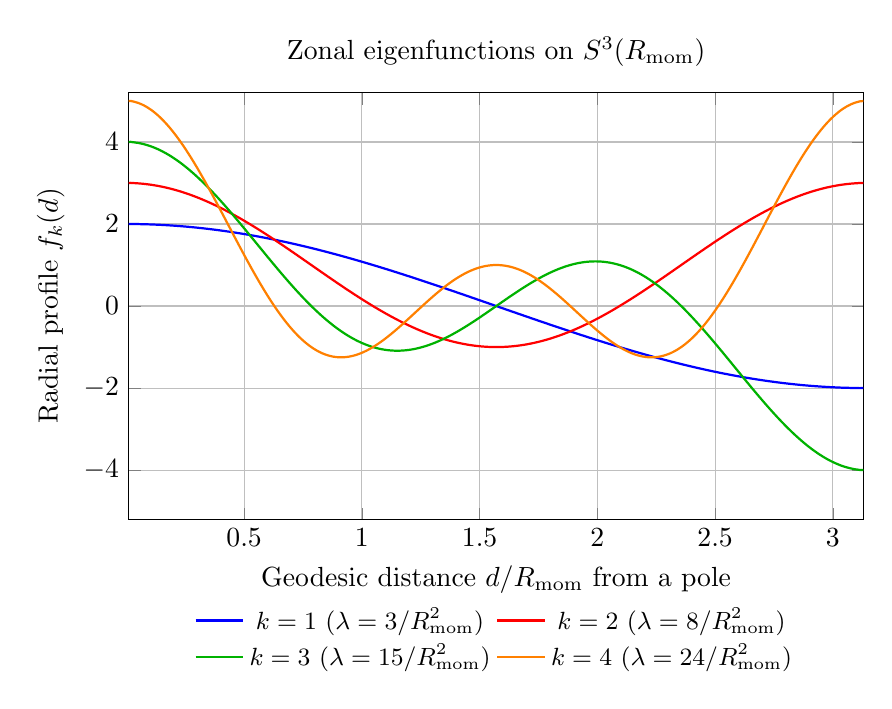
\begin{tikzpicture}
\begin{axis}[
  width=0.9\linewidth,
  height=7cm,
  xlabel={Geodesic distance \(d/\Rmom\) from a pole},
  ylabel={Radial profile \(f_k(d)\)},
  grid=major,
  title={Zonal eigenfunctions on \(S^3(\Rmom)\)},
  xmin=0.01, xmax=3.13,
  ymin=-5.2, ymax=5.2,
  domain=0.01:3.13,
  samples=400,
  unbounded coords=jump,
  legend style={
    at={(0.5,-0.18)},
    anchor=north,
    font=\small,
    draw=none
  },
  legend columns=2
]
\addplot[thick,blue,smooth] {sin(deg(2*x))/sin(deg(x))};
\addplot[thick,red,smooth] {sin(deg(3*x))/sin(deg(x))};
\addplot[thick,green!70!black,smooth] {sin(deg(4*x))/sin(deg(x))};
\addplot[thick,orange,smooth] {sin(deg(5*x))/sin(deg(x))};

\legend{
  \(k=1\) \((\lambda=3/\Rmom^2)\),
  \(k=2\) \((\lambda=8/\Rmom^2)\),
  \(k=3\) \((\lambda=15/\Rmom^2)\),
  \(k=4\) \((\lambda=24/\Rmom^2)\)
}
\end{axis}
\end{tikzpicture}

\caption[Radial profiles of the first four zonal eigenfunctions on \(S^3\)]{%
\textbf{Radial profiles of the first four zonal eigenfunctions on \(S^3(\Rmom)\).}
These functions depend only on the geodesic distance \(d\) from a fixed pole and have the form
\(f_k(d)\propto \sin((k+1)d/\Rmom)/\sin(d/\Rmom)\).
The removable endpoint singularities at \(d=0\) and \(d=\pi\Rmom\) are omitted in the plot.
The number of zeros in \(0<d<\pi\Rmom\) is exactly \(k\), corresponding to the eigenvalue
\(\lambda_k = k(k+2)/\Rmom^2\)
of the Laplace--Beltrami operator.
Higher \(k\) oscillate faster, as required by the Peter--Weyl decomposition on \(\mathrm{SU}(2)\).%
}
\label{fig:eigenfunctions}
\end{figure}


\subsection{Commutants, multiplicity spaces, and isotypic blocks}
\label{p1:subsec:commutants-multiplicity}

Let $V$ be a finite-dimensional complex Hilbert space with a unitary representation $\rho:G\to U(V)$ of a
compact group $G$. Write $\End_G(V)$ for the commutant algebra:
\[
\End_G(V):=\{A\in\End(V)\;:\;A\rho(g)=\rho(g)A\ \forall g\in G\}.
\]

\begin{theorem}[Isotypic decomposition and commutant factorization]
\label{p1:thm:isotypic-commutant}
There is a canonical isotypic decomposition
\[
V\;\cong\;\bigoplus_{\pi\in\widehat G}\; M_\pi\otimes V_\pi,
\qquad
M_\pi:=\Hom_G(V_\pi,V),
\]
where $V_\pi$ runs over irreducible unitary representations and $\dim M_\pi=m_\pi$. Under
this canonical identification one has an isomorphism of algebras
\[
\End_G(V)\;\cong\;\bigoplus_{\pi\in\widehat G}\;\End(M_\pi)\otimes \mathbf 1_{V_\pi}.
\]
After choosing bases of the multiplicity spaces $M_\pi$, this becomes
\(\bigoplus_{\pi\in\widehat G}M_{m_\pi}(\CC)\otimes\mathbf 1_{V_\pi}\).
\end{theorem}

\begin{proof}
This is standard Peter--Weyl/complete reducibility. The evaluation map
\(M_\pi\otimes V_\pi\to V\), \(f\otimes v\mapsto f(v)\), identifies the \(\pi\)-isotypic summand canonically with \(M_\pi\otimes V_\pi\), and the direct sum over irreducible classes gives the displayed decomposition. Schur's lemma then implies that a $G$-equivariant endomorphism acts arbitrarily on each multiplicity space and as the identity on the corresponding irreducible factor, giving \(\End_G(V)\cong\bigoplus_\pi \End(M_\pi)\otimes\mathbf 1_{V_\pi}\).
\end{proof}


\section{Scaling and Dimensional Analysis}
\label{p1:sec:scaling-analysis}


\begin{proposition}[Homothetic scaling laws on \(S^3(\Rmom)\)]
\label{p1:prop:homothetic-scaling-laws}
Under the radius change \(\Rmom\to\lambda\Rmom\), equivalently the metric
homothety \(g\to\lambda^2g\) with \(\lambda>0\), the following scaling laws
hold.
\begin{center}
\small
\setlength{\tabcolsep}{3pt}
\renewcommand{\arraystretch}{1.18}

\begin{tabular}{|
  L{3.6cm}|
  L{\dimexpr\linewidth-3.6cm-4\tabcolsep-3\arrayrulewidth\relax}|
}
\hline
\textbf{Quantity} & \textbf{Scaling under \(\Rmom \to \lambda \Rmom\)} \\
\hline

Metric \(g_{ij}\)
& \(g \to \lambda^2 g\) \\
\hline

Volume \(\mathrm{vol}_{S^3}\)
& \(\mathrm{vol} \to \lambda^3 \mathrm{vol}\) \\
\hline

Sectional curvature \(K\)
& \(K \to \lambda^{-2}K\) \\
\hline

Ricci tensor \(\mathrm{Ric}\)
& \(\mathrm{Ric}_{\lambda^2 g}=\mathrm{Ric}_g\) as a \((0,2)\)-tensor \\
\hline

Scalar curvature \(\mathrm{scal}\)
& \(\mathrm{scal} \to \lambda^{-2}\mathrm{scal}\) \\
\hline

Laplacian eigenvalues \(\lambda_k\)
& \(\lambda_k \to \lambda^{-2}\lambda_k\) \\
\hline

Dirac eigenvalues \(\mu_k\)
& \(\mu_k \to \lambda^{-1}\mu_k\) \\
\hline

Heat kernel
& For \(K_{\Rmom}(t,x,y)\), after radial homothety identification,
  \[
    K_{\lambda\Rmom}(t,\lambda x,\lambda y)
    =
    \lambda^{-3}
    K_{\Rmom}(\lambda^{-2}t,x,y).
  \]
\\[-1.5ex]
\hline

Minimal Reeb period \(\mathcal A_{\min}\)
& \(\mathcal A_{\min} \to \lambda\mathcal A_{\min}\) \\
\hline

\end{tabular}
\end{center}
\end{proposition}

\begin{proof}
All entries are the standard homothetic scaling laws.  Lengths scale by \(\lambda\), volumes by \(\lambda^3\), scalar curvature and sectional curvature by \(\lambda^{-2}\), the scalar Laplacian by \(\lambda^{-2}\), and the Dirac operator by \(\lambda^{-1}\).  The heat-kernel law follows from preservation of total heat under the radial homothety together with parabolic time scaling \(t\mapsto\lambda^2t\).  The Reeb period/action scales linearly because \(\eta=\Rmom\eta_0\).
\end{proof}

\subsection{Coordinate-Invariant Formulations}
\label{p1:subsec:coordinate-invariant}

Many structures have coordinate-invariant formulations:

\paragraph{Contact structure.} The contact distribution $\mathcal{H} = \ker\eta$ is maximally non-integrable: $\eta \wedge d\eta \neq 0$ everywhere. This is equivalent to $\mathcal{H}$ being a contact structure in the sense of differential topology.

\paragraph{Reeb field.} The vector field $\xi_\eta$ satisfying $\eta(\xi_\eta)=1$ and $d\eta(\xi_\eta,\cdot)=0$. On $S^3$, this geometric structure generates the Hopf fibration.

\paragraph{Hopf fibration.} The $U(1)$-principal bundle $\Sone\hookrightarrow S^3(\Rmom)\xrightarrow{\pi} S^2$ carries the dimensionless connection 1-form $\eta_0:=\eta/\Rmom$ and basic curvature $F_0:=d\eta_0=\pi^*\omega$. Under the orientation convention fixed in Proposition~\ref{p1:prop:contact-normalization}, the descended base curvature satisfies
\[
\int_{S^2}\omega=2\pi,
\qquad
c_1(P)=[\omega/2\pi]\in H^2(S^2;\ZZ),
\]
so the Hopf bundle has Euler number \(1\).

\paragraph{Seifert fibration structure.} The Hopf fibration is the regular circle bundle over $S^2$ with Euler number $e=1$ in the present convention.  Equivalently, it is the principal $\Sone$-bundle over $S^2$ with Chern class $c_1=1$.  The precise tuple of Seifert invariants is convention-dependent and changes sign under orientation reversal.


\begin{table}[htbp]
\centering
\begingroup
\small
\setlength{\tabcolsep}{4pt}
\renewcommand{\arraystretch}{1.25}
\resizebox{\textwidth}{!}{%
\begin{tabular}{|l|c|p{5.4cm}|}
\hline
\textbf{Invariant} & \textbf{Expression} & \textbf{Value at \(\Rmom=1\)} \\
\hline
Riemannian volume & $\mathrm{Vol}(S^3(\Rmom))$ & \(2\pi^2\) \\
Normalized Maurer--Cartan real representative & \( |\CS(\theta)| \) & \(1\) as a real representative; class \(0\) in \(\RR/\ZZ\) \\
First Chern class & \(c_1\) & \(1\) \\
Minimal Reeb period & \(\mathcal A_{\min}\) & \(2\pi\) \\
Yamabe invariant & \(Y(S^3)\) & \(6(2\pi^2)^{2/3}\) \\
Spectral gap (Laplacian) & \(\lambda_1\) & \(3\) \\
Spectral gap (Dirac) & \(|\mu_0|\) & \(3/2\) \\
Clifford carrier dimensions & \(\bigl(\dim_\RR\overline{\Cl}_{\mathrm{car}},\dim_\RR\Cl_{\mathrm{car}}\bigr)\) & \((7,8)\) \\
Carrier interface inverse & \(r_{\rm HC}(r_{\rm HC}-1)\) & \(56\) \\
Exterior-degree dimensions & \(\dim \Lambda^k\RR^3\) & \((1,3,3,1)\) \\
Round Dirac eta invariant & \(\eta_D(0)\) & \(0\) \\
\hline
\end{tabular}%
}
\caption[Fundamental Hopf-fibered invariants]{Fundamental Hopf-fibered invariants.}
\label{p1:tab:invariants-summary}
\TableNotes{Values refer to the normalized round and chosen Hopf
structures.  Discrete exceptional-group and polytope data are collected in
Paper~I-B.}
\endgroup
\end{table}
\noindent\textbf{Scaling with radius.} 
Table~\ref{p1:tab:invariants-summary} lists values at $\Rmom=1$. For general $S^3(\Rmom)$, $\mathrm{Vol}(S^3(\Rmom))=2\pi^2\Rmom^3$, the Hopf fiber period scales as \(\mathcal A_{\min}=2\pi \Rmom\).


\part{Topological and Symplectic Reference Structures}
\label{p1:part:topological-symplectic}

\section{Canonical Topological and Symplectic Structures}
\label{p1:sec:canonical-topological}
After a Hopf representative and its orientation convention have been fixed, the
round \(3\)-sphere \(S^3(\Rmom)\) carries the following topological,
bundle-theoretic, and contact structures.  They are canonical relative to that
representative, while their conjugacy-invariant content belongs to the
underlying Hopf class.  These structures are summarized in
Table~\ref{p1:tab:canonical-topological}.


\begin{table}[p]
\centering
\footnotesize
\begingroup
\renewcommand{\arraystretch}{1.2}
\setlength{\tabcolsep}{2pt}

\begin{tabular}{|
  L{2.7cm}|
  L{\dimexpr\linewidth-2.7cm-3.5cm-2.25cm-8\tabcolsep-5\arrayrulewidth\relax}|
  L{3.5cm}|
  C{2.25cm}|
}
\hline
\textbf{Structure} & \textbf{Mathematical Statement} & \textbf{Description} & \textbf{Ref.} \\
\hline

Principal \(U(1)\)-bundle
& \(\Sone \hookrightarrow S^3(\Rmom) \overset{\pi}{\to} S^2\) with connection
  \(\eta_0:=\eta/\Rmom\).
& Chosen representative of the Hopf conjugacy class
& \S\ref{p1:der:hopf-connection} \\
\hline

First Chern class
& \(c_1 = 1 \in H^2(S^2;\ZZ)\).
& Generator of cohomology, independent of radius
& Prop.~\ref{p1:prop:contact-normalization} \\
\hline

Chern class charge
& \(\displaystyle\int_{S^2}\omega = 2\pi\) in the chosen base orientation.
& Hopf bundle realizes \(c_1=[\omega/2\pi]=1\)
& Prop.~\ref{p1:prop:contact-normalization} \\
\hline

Tight contact structure
& \(\eta \wedge d\eta = \frac{2}{\Rmom}\vol_{S^3(\Rmom)} > 0\) gives the
  contact condition; standard ball fillability gives tightness, and the
  positive tight structure on \(S^3\) is unique up to isotopy.
& Local contact condition plus global filling/classification
& Prop.~\ref{p1:prop:standard-contact-fill-tight} \\
\hline

Hopf fiber \(U(1)\) embedding
& \(U(1)_L\subset\operatorname{Sp}in(4)\cong\SU(2)_L\times\SU(2)_R\) in the fixed
  common-phase convention.
& One-sided phase rotation \(q\mapsto e^{i\alpha}q\) along Hopf fibers
& \S\ref{p1:der:diagonal-embedding} \\
\hline

Metric-scaled minimal Reeb period
& \(\mathcal A_{\min}=2\pi \Rmom\) for \(\eta\), while it is \(2\pi\) for
  \(\eta_0\).
& Minimal action of a closed Reeb orbit for \(\eta=\Rmom\eta_0\)
& \S\ref{p1:der:capacities} \\
\hline

Symplectic base normalization
& \(\displaystyle\int_{S^2}\omega = 2\pi\), so
  \([\omega/2\pi]=c_1\).  This is the
  Chern--\allowbreak Weil/prequantization curvature form, not the Riemannian
  area form of \(S^2(\Rmom/2)\), whose total area is \(\pi\Rmom^2\).
& Normalized symplectic form on base
& Prop.~\ref{p1:prop:contact-normalization} \\
\hline

Boothby--Wang structure
& \(d\eta_0=\pi^*\omega\), \([\omega/2\pi]=c_1(P)\).
& Regular contact form as prequantization bundle
& \S\ref{p1:der:boothby-wang} \\
\hline

Homotopy generator
& \([\pi]\) generates \(\pi_3(S^2)\cong\ZZ\).
& Long exact sequence of the fibration
& \S\ref{p1:der:hopf-homotopy} \\
\hline

\end{tabular}

\caption[Topological and symplectic structures of a Hopf representative]{Topological and symplectic structures of a Hopf representative.}
\label{p1:tab:canonical-topological}
\TableNotes{The rows record structures relative to the displayed Hopf
representative.  Their bundle-isomorphism class and Chern magnitude are
invariant under conjugating the representative; the embedded axis and
oriented sign are not.}
\endgroup
\end{table}

\begin{proposition}[Standard filling, tightness, and uniqueness]
\label{p1:prop:standard-contact-fill-tight}
Let
\[
  \lambda_{\rm std}
  :=\frac12\sum_{a=1}^{2}(x_a\,dy_a-y_a\,dx_a)
\]
on \(\CC^2\cong\RR^4\), and let \(B^4(\Rmom)\) have boundary
\(S^3(\Rmom)\).  With the Hopf-coordinate convention of this paper,
\[
  \left.\lambda_{\rm std}\right|_{S^3(\Rmom)}
  =\frac{\Rmom^2}{4}
   (d\psi+\cos\theta\,d\phi)
  =\frac{\Rmom}{2}\eta.
\]
Consequently the rescaled Liouville form
\[
  \lambda_{\Rmom}:=\frac{2}{\Rmom}\lambda_{\rm std}
\]
satisfies
\[
  \left.\lambda_{\Rmom}\right|_{S^3(\Rmom)}=\eta,
\]
and \((B^4(\Rmom),d\lambda_{\Rmom})\) is a strong exact symplectic filling
of \((S^3(\Rmom),\ker\eta)\).  Hence the standard contact structure is
tight.  Moreover, the positive tight contact structure on \(S^3\) is unique
up to isotopy.
\end{proposition}

\begin{proof}
The boundary restriction follows by substituting the standard Hopf
parametrization of \(S^3(\Rmom)\) into \(\lambda_{\rm std}\).  Multiplication
by the positive constant \(2/\Rmom\) preserves nondegeneracy of
\(d\lambda_{\rm std}\), and the radial Liouville vector remains transverse
to the boundary, so the displayed ball is a strong exact filling with
boundary contact form \(\eta\).  Strong symplectic fillability implies
tightness; see \cite{geiges2008contact}.  Uniqueness up to isotopy is
Eliashberg's tight-\(S^3\) classification
\cite{Eliashberg1992TightS3}.
\end{proof}

\subsection{\texorpdfstring{Chern--Simons invariant on $S^3$}{Chern--Simons invariant on S3}}
\label{p1:sec:cs-invariant}

On $S^3 \cong \SU(2)$ the Maurer--Cartan form canonically produces a distinguished
integral cohomology class in $H^3(S^3;\ZZ)$, and the corresponding
Chern--Simons functional is naturally defined only after fixing a normalization.
The orientation/sign convention is the one fixed in Convention~\ref{p1:conv:global-orientation-signs}.
We therefore state the invariant in a convention-robust way.

\begin{definition}[Normalized Chern--Simons 3-form and functional]\label{p1:def:cs-normalized}
Let \(G=\SU(2)\), let \(\mathfrak g=\mathfrak{su}(2)\), and let
\(A\in\Omega^1(S^3;\mathfrak g)\) be the globally defined base gauge potential
of a connection in a chosen trivialization over \(S^3\).
In the defining matrix representation, set
\[
\cs(A)
:=\frac{1}{8\pi^2}\Tr\!\left(A\wedge dA+\frac{2}{3}A\wedge A\wedge A\right),
\qquad
\CS(A):=\int_{S^3}\cs(A).
\]
(Here $A\wedge A$ denotes the wedge product together with matrix multiplication.)
\end{definition}

\begin{proposition}[Gauge ambiguity]\label{p1:prop:cs-gauge-ambiguity}
For a gauge transformation $g:S^3\to \SU(2)$, write
\[
A^g:=g^{-1}Ag+g^{-1}dg.
\]
Define the degree in the matching trace/orientation convention by
\[
\deg(g):=-\frac{1}{24\pi^2}\int_{S^3}\Tr\bigl((g^{-1}dg)^{\wedge 3}\bigr)\in\ZZ.
\]
Then, with the sign fixed by this convention and by the normalization in
Definition~\ref{p1:def:cs-normalized},
\[
\CS(A^g)-\CS(A)=\deg(g).
\]
Equivalently, $\CS(A)$ is well-defined as an element of $\RR/\ZZ$.
\end{proposition}

\begin{proof}
The standard transgression identity gives
\[
\cs(A^g)-\cs(A)
=d\,\eta(A,g)-\frac{1}{24\pi^2}\Tr\bigl((g^{-1}dg)^{\wedge 3}\bigr),
\]
for an explicit globally defined two-form \(\eta(A,g)\).  Since \(S^3\) is closed,
the exact term integrates to zero, while the final integral is precisely
\(\deg(g)\) by the convention just stated. Hence \(\CS(A^g)-\CS(A)=\deg(g)\in\ZZ\),
and \(\CS(A)\) is well-defined modulo \(\ZZ\).  See e.g.\ \cite{ChernSimons1974,bott1982differential}.
\end{proof}

\begin{theorem}[Maurer--Cartan generator]\label{p1:thm:mc-generator}
Let $\theta:=g^{-1}dg$ be the Maurer--Cartan form on $\SU(2)\cong S^3$.
Then
\[
\cs(\theta)=-\frac{1}{24\pi^2}\Tr(\theta\wedge\theta\wedge\theta)
\]
is a bi-invariant closed 3-form representing the de Rham image of an integral generator of $H^3(S^3;\ZZ)$
(with sign determined by orientation). In particular, as a chosen real normalized representative,
\[
\CS(\theta)=\pm 1.
\]
Here \(\theta=g^{-1}dg\) is a pure-gauge connection representative.  Its real Chern--Simons value records the winding normalization of that representative; as a gauge-invariant Chern--Simons value modulo \(\ZZ\), the class is \(0\in\RR/\ZZ\).
\end{theorem}

\begin{proof}
The Maurer--Cartan equation $d\theta+\theta\wedge\theta=0$ gives
\[
\cs(\theta)
=\frac{1}{8\pi^2}\Tr\!\left(\theta\wedge(-\theta\wedge\theta)+\frac{2}{3}\theta\wedge\theta\wedge\theta\right)
=-\frac{1}{24\pi^2}\Tr(\theta^{\wedge 3}).
\]
The 3-form $\frac{1}{24\pi^2}\Tr(\theta^{\wedge 3})$ is the standard integral Cartan 3-form on $\SU(2)$,
whose integral over $S^3$ is $\pm 1$ depending on orientation; see \cite{bott1982differential}.
\end{proof}

\begin{corollary}[Relation to the Riemannian volume form]\label{p1:cor:cs-volume-relation}
For the round metric on $S^3(\Rmom)$ with its standard orientation, the generator in
Theorem~\ref{p1:thm:mc-generator} is proportional to the Riemannian volume form:
\[
\frac{1}{24\pi^2}\Tr(\theta^{\wedge 3})
=\pm \frac{1}{2\pi^2\Rmom^3}\,\vol_{S^3(\Rmom)}.
\]
Consequently, its integral is $\pm 1$ for all $\Rmom>0$.
\end{corollary}

\begin{proof}
Both sides are bi-invariant top-degree forms on \(SU(2)\cong S^3\), hence differ by a constant. The normalization of the Cartan generator gives integral \(\pm1\), while \(\Vol(S^3(\Rmom))=2\pi^2\Rmom^3\); this fixes the proportionality constant as displayed.
\end{proof}


\begin{remark}
Any unnormalized choice (e.g.\ omitting the prefactor $1/(8\pi^2)$, or changing the trace/bilinear form) rescales $\CS$ by a fixed constant. Therefore numerical identities such as $|\int \mathrm{CS}| = c\cdot\Vol(S^3)$ are \emph{convention-dependent} and should not be presented as universal. The convention-robust statement is that $\cs(\theta)$ represents the generator of $H^3(S^3;\ZZ)$ and integrates to $\pm 1$.
\end{remark}


\subsection{Hopf Fibration as Principal Connection}
\label{p1:der:hopf-connection}
The dimensionless principal connection is $\eta_0:=\eta/\Rmom$ (cf. Proposition~\ref{p1:prop:contact-normalization}); the metric-scaled contact form used elsewhere is $\eta=\Rmom\,\eta_0$.
\begin{remark}[Holonomy of the Hopf connection]
Let \(\gamma\subset S^2\) be a loop and let \(s\) be a local section over a
spanning surface \(\Sigma\subset S^2\) with \(\partial\Sigma=\gamma\).  The
holonomy of the principal connection \(\eta_0\) is
\[
\mathrm{Hol}(\gamma)
=\exp\Bigl(i\oint_{\gamma}s^*\eta_0\Bigr)
=\exp\Bigl(i\int_{\Sigma}s^*d\eta_0\Bigr)
=\exp\Bigl(i\int_{\Sigma}\omega\Bigr),
\]
up to the orientation convention fixed in Proposition~\ref{p1:prop:contact-normalization}, where
\(\omega\) is the normalized integral prequantization curvature form representing the Hopf
Chern class; it differs by a constant scale from the Riemannian area form on \(S^2(\Rmom/2)\).  Thus the holonomy depends only on the enclosed symplectic area
modulo \(2\pi\). With the convention that the Lie-algebra-valued connection is \(i\eta_0\), this gives the displayed sign; the opposite convention for parallel transport replaces the holonomy by its inverse.
\end{remark}

\subsection{Boothby--Wang and prequantization}
\label{p1:der:boothby-wang}

\begin{theorem}[regular Boothby--Wang structure]
\label{p1:thm:boothby-wang-hopf}
Let \(\eta_0=\eta/\Rmom\) be the dimensionless Hopf contact form on \(S^3\), with
the base orientation chosen so that the Hopf curvature convention satisfies
\(d\eta_0=\pi^*\omega\) and hence \([\omega/2\pi]=c_1(P)=+1\). Then:
\begin{enumerate}
    \item \((S^3,\eta_0)\) is a regular contact manifold.
    \item Its Reeb flow is the free circle action of the Hopf fibration.
    \item There exists a symplectic form \(\omega\) on \(S^2\) such that
    \[
    d\eta_0=\pi^*\omega,
    \qquad
    [\omega/2\pi]=c_1(P)\in H^2(S^2;\ZZ).
    \]
\end{enumerate}
Hence \(S^3\) is the Boothby--Wang, equivalently prequantization, circle bundle of
the integral symplectic surface \((S^2,\omega)\).
\end{theorem}

\begin{proof}
With the stated base orientation, this is the basic Boothby--Wang construction
applied to the Hopf fibration; reversing the base orientation would reverse the
sign of the displayed Chern-class representative.  See
\cite{BoothbyWang1958,geiges2008contact}.
\end{proof}


\subsection{First Chern Class and Non-Triviality}
\label{p1:der:chern-class}
The Chern class $c_1=1$ implies the bundle is topologically non-trivial.
\begin{remark}[Nonexistence of global sections]
Because \(c_1\neq 0\), the Hopf principal \(U(1)\)-bundle is topologically
nontrivial and therefore admits no global smooth section.
\end{remark}

\subsection{Homotopy exact sequence and the Hopf map}
\label{p1:der:hopf-homotopy}

\begin{theorem}[homotopy exact sequence of the Hopf fibration]
\label{p1:thm:hopf-homotopy-exact-sequence}
For the fibration
\[
\Sone \hookrightarrow S^3 \xrightarrow{\pi} S^2,
\]
the long exact sequence in homotopy yields:
\[
\pi_2(S^2)\xrightarrow{\partial}\pi_1(S^1)
\]
is an isomorphism, and
\[
\pi_3(S^3)\xrightarrow{\ \pi_*\ }\pi_3(S^2)
\]
is an isomorphism. Consequently,
\[
\pi_3(S^2)\cong \ZZ,
\]
and the Hopf map represents a generator.
\end{theorem}

\begin{proof}
Apply the long exact sequence of homotopy groups to the Hopf fibration and use
\(\pi_2(S^1)=\pi_3(S^1)=0\), \(\pi_3(S^3)\cong\ZZ\), and \(\pi_1(S^3)=0\); see
\cite{steenrod1951topology,bott1982differential,hopf1931abbildung}.
\end{proof}


\subsection{\texorpdfstring{Hopf fiber $U(1)$ and the base isotropy subgroup}{Hopf fiber U(1) and the base isotropy subgroup}}
\label{p1:der:diagonal-embedding}
Under the $\operatorname{Sp}in(4)$ action $(a,b):q\mapsto a\,q\,b^{-1}$ on
$S^3\simeq\SU(2)$, the Hopf fiber action in the common-phase convention fixed in
Proposition~\ref{p1:prop:contact-normalization} is the one-sided embedded circle
$U(1)\subset\SU(2)_L$, acting by $q\mapsto e^{i\alpha}q$.  In the opposite Hopf
handedness convention the analogous fiber circle lies in $\SU(2)_R$.  This
fiber circle should not be confused with the diagonal subgroup
$\Delta\SU(2)\subset\SU(2)_L\times\SU(2)_R$.  The diagonal subgroup acts on
$S^3\simeq\SU(2)$ by conjugation and its quotient by $\{\pm1\}$ is abstractly
$\SO(3)$, appearing as the isotropy representation at the identity.  For the
selected common-phase Hopf convention, however, the base rotation group is
represented by the right factor
\[
\SU(2)_R/\{\pm1\}\cong\SO(3),
\]
while the vertical fiber action is the selected circle $U(1)\subset\SU(2)_L$.
\begin{proposition}[Averaging over oriented Hopf representatives yields an isotropic ensemble]
\label{p1:prop:hopf-ensemble-isotropy}
The moduli space of \emph{oriented} Hopf representatives on the round $S^3$
compatible with the metric, orientation, and a chosen twistor handedness
component (self-dual or anti-self-dual) is the homogeneous space
\[
\mathcal M_{\mathrm{Hopf}}\cong \SO(4)/\mathrm U(2)\cong S^2.
\]
Each handedness component is such an $S^2$. If both left- and right-handed Hopf fibrations are included, the full oriented moduli space is the disjoint union of two such components. The two handedness components are separate under the orientation-preserving $\SO(4)$-action; allowing orientation-reversing elements would interchange them.
For the remainder of this proposition, \(\mathcal M_{\mathrm{Hopf}}\) denotes one fixed handedness component, and \(\mu\) denotes its unique normalized \(\SO(4)\)-invariant probability measure. Then the averaging functional
\[
F\longmapsto \overline{F}:=\int_{\mathcal M_{\mathrm{Hopf}}}F(h)\,d\mu(h)
\]
on integrable scalar functions \(F:\mathcal M_{\mathrm{Hopf}}\to \RR\) is
\(\SO(4)\)-invariant. More generally, if \(A(h)\) is a tensor-valued function
transforming equivariantly under the \(\SO(4)\)-action, then its average lies in
the \(\SO(4)\)-invariant subspace of the corresponding representation. If both handedness components are included, an \(\SO(4)\)-invariant probability measure is obtained only after choosing the relative weights of the two component measures; the equal-weight measure is a symmetric convention, not a consequence of invariance alone.
\end{proposition}

\begin{proof}
For a fixed twistor handedness component, the round metric identifies that
component of the family of compatible oriented Hopf representatives with the
homogeneous space $\SO(4)/\mathrm U(2)$, whose stabilizer is the subgroup
preserving the corresponding orthogonal complex structure.  Including the opposite handedness gives a second, disjoint copy rather than a connected enlargement of this component; the two handedness components are separate under the orientation-preserving \(\SO(4)\)-action, while allowing orientation-reversing elements would interchange them. For the chosen component,
$\mathcal M_{\mathrm{Hopf}}$ is compact and homogeneous, so it carries a unique
normalized $\SO(4)$-invariant probability measure $\mu$. On the disjoint union of the two handedness components, the invariant probability measures are precisely the convex combinations \(\alpha\mu_+ +(1-\alpha)\mu_-\), \(0\leq\alpha\leq1\), of the two component measures; hence a relative weight is additional data.

For any \(g\in\SO(4)\),
\[
\int_{\mathcal M_{\mathrm{Hopf}}}F(g\cdot h)\,d\mu(h)
=
\int_{\mathcal M_{\mathrm{Hopf}}}F(h)\,d\mu(h)
\]
by invariance of \(\mu\). Hence the scalar averaging functional is
\(\SO(4)\)-invariant.

If $A(h)$ is tensor-valued and equivariant, then
\[
\overline{A}:=\int_{\mathcal M_{\mathrm{Hopf}}}A(h)\,d\mu(h)
\]
is fixed by the induced representation of $\SO(4)$, so
$\overline{A}$ lies in the invariant subspace.
\end{proof}

\begin{corollary}[Canonical Hopf class but no canonical Hopf axis]
\label{p1:cor:hopf-class-no-axis}
For a fixed handedness, all compatible oriented Hopf representatives of the
oriented round \(S^3\) lie in one \(\SO(4)\)-orbit, but this orbit has no
\(\SO(4)\)-fixed point.  Equivalently, after the Lie-group structure is fixed,
maximal tori \(T\simeq U(1)\subset SU(2)\) exist and are mutually conjugate.
After a generator orientation is chosen, each quotient
\[
        T\backslash SU(2)\simeq S^2
\]
defines the left-orbit Hopf fibration used below (equivalently,
\(SU(2)/T\simeq S^2\) after inversion), but the unmarked round group selects no particular
\(T\).  Any one such fibration may be fixed as an atlas representative.
Conjugate representatives have isomorphic bundle, contact, spectral, and
Chern-magnitude data; convention-dependent axes, left/right labels, and
oriented signs must be transported with the representative.
\end{corollary}

\begin{proof}
The first statement follows from
\(\mathcal M_{\mathrm{Hopf}}\cong\SO(4)/U(2)\cong S^2\): a nontrivial
homogeneous orbit has no point fixed by the transitive \(\SO(4)\)-action.
The maximal-torus formulation is the standard homogeneous realization
\(U(1)\backslash SU(2)\cong S^2\), equivalently
\(SU(2)/U(1)\cong S^2\) under inversion.  Conjugation carries one maximal torus and its
homogeneous bundle to any other, proving the final statement.
\end{proof}


\begin{theorem}[Chosen Hopf/Reeb abelian generator]
\label{p1:thm:canonical-hopf-u1}
Fix the oriented round sphere \(S^3(\Rmom)\) together with one compatible Hopf fibration
\[
\Sone \hookrightarrow S^3 \xrightarrow{\pi} S^2
\]
and let \(\eta_0\) be the dimensionless principal connection. Let
\[
X_H:=\Rmom\xi_\eta=2\partial_\psi,
\qquad
\eta_0(X_H)=1,
\]
where \(\xi_\eta\) is the metric-normalized Reeb field of \(\eta=\Rmom\eta_0\).
Then:
\begin{enumerate}
    \item the dimensionless Reeb/principal generator \(X_H\) generates the free isometric \(\Sone\)-action along the Hopf fibers;
    \item any smooth vector field \(X\) tangent to the Hopf fibers and satisfying \(\eta_0(X)=1\) coincides with \(X_H\);
    \item after fixing orientation, the infinitesimal global abelian fiber generator is unique.
\end{enumerate}
Equivalently, the first-order operator \(i\mathcal L_{X_H}\) is the unique selected abelian generator attached to the chosen Hopf bundle, up to overall sign before orientation is fixed. In the metric/action normalization the same geometric direction is generated by \(\xi_\eta=\Rmom^{-1}X_H\), with closed-orbit action \(2\pi\Rmom\).
\end{theorem}

\begin{proof}
By the regular Boothby--Wang structure, the Hopf fibers are precisely the Reeb orbits of the dimensionless contact form \(\eta_0\), whose Reeb field is \(X_H\). If \(X\) is tangent to the fibers, then \(\pi_*X=0\), so
\[
\iota_X d\eta_0 = 0
\]
because \(d\eta_0=\pi^*\omega\) is horizontal. Together with \(\eta_0(X)=1\), this is exactly the defining property of the Reeb field of \(\eta_0\). Hence \(X=X_H\). The remaining sign ambiguity is removed once the fiber orientation is fixed.
\end{proof}

\subsection{Closed Reeb orbits and minimal action}
\label{p1:der:capacities}

For the standard contact form \(\eta\), every Reeb orbit is a Hopf fiber and is
closed of period \(2\pi\Rmom\). Hence the minimal period, equivalently the minimal
action among closed Reeb orbits, is
\[
\mathcal A_{\min}=2\pi\Rmom.
\]

\begin{remark}[Form-level rigidity versus structure-level flexibility]
The all-periodic Hopf flow is a property of the distinguished contact form
\(\eta_0\), not merely of the underlying contact structure
\[
\xi_{\mathrm{std}}=\ker\eta_0.
\]
The same standard tight contact structure on \(S^3\) admits other contact forms
with qualitatively different Reeb dynamics, including forms with dense or ergodic
Reeb orbits.
\cite{CasalsSpacil2015}
\end{remark}
\begin{theorem}[Hopf normalization package]
\label{p1:thm:hopf-normalization-package}
For the chosen Hopf bundle on the round sphere \(S^3(\Rmom)\) with dimensionless connection
\[
\eta_0:=\eta/\Rmom,
\]
the following normalization data are fixed relative to the chosen Hopf bundle, orientation convention, trace convention, and radius \(\Rmom\):
\begin{enumerate}
    \item
    \[
    [\omega/2\pi]=c_1(P)=1\in H^2(S^2;\ZZ),
    \qquad
    \int_{S^2}\omega = 2\pi;
    \]
    \item for the dimensionless contact form \(\eta_0\), the Reeb generator \(X_H\)
    has period and \(\eta_0\)-action
    \[
    2\pi.
    \]
    Equivalently, for the metric-scaled contact form \(\eta=\Rmom\eta_0\)
    and metric-normalized Reeb field \(\xi_\eta=\Rmom^{-1}X_H\), every Hopf
    fiber has period and \(\eta\)-action
    \[
    \mathcal A_{\min}=2\pi\Rmom;
    \]
    \item the normalized Maurer--Cartan 3-form
    \[
    \frac{1}{24\pi^2}\Tr(\theta^{\wedge 3})
    \]
    represents the de Rham image of an integral generator of \(H^3(S^3;\ZZ)\) and integrates to \(\pm 1\); this is a real normalized representative, while the corresponding Chern--Simons class modulo \(\ZZ\) is \(0\);
    \item once the chosen Hopf bundle, orientation convention, trace convention, and \(\Rmom\) are fixed, the base symplectic scale, fiber scale, and integral 3-form scale carry no further free normalization.
\end{enumerate}
\end{theorem}

\begin{proof}
Item (1) is the Boothby--Wang normalization together with the first Chern class calculation. For Item (2), the dimensionless generator \(X_H\) is normalized by \(\eta_0(X_H)=1\), so a principal-circle orbit has parameter period and \(\eta_0\)-action \(2\pi\). Scaling the contact form to \(\eta=\Rmom\eta_0\) rescales the normalized Reeb field to \(\xi_\eta=\Rmom^{-1}X_H\) and therefore rescales the corresponding closed-orbit period/action to \(2\pi\Rmom\). Item (3) is Theorem~\ref{p1:thm:mc-generator}. Item (4) is the collection of these selected topological, contact-form, metric-scale, and trace/orientation normalizations.
\end{proof}

\begin{corollary}[Oriented primitive lattice of the chosen Hopf flow]
\label{p1:cor:positive-reeb-lattice}
For the chosen Hopf bundle and orientation of
Theorem~\ref{p1:thm:hopf-normalization-package}, let
\[
 \exp_H:\mathbb R X_H\longrightarrow U(1)_H
\]
denote the Reeb/principal-circle exponential.  Its period lattice is
\[
 \Lambda_H:=\ker(\exp_H)=2\pi\mathbb Z X_H.
\]
The element
\[
 \boxed{\tau_H^+:=2\pi X_H}
\]
is the unique positive primitive generator of this lattice.  Equivalently,
the universal-cover parameter \(s\) is positively oriented by
\[
 s\longmapsto\exp_H(sX_H),\qquad s\ \text{increasing}.
\]
This is the oriented flow datum of the chosen Hopf branch, with its stated
geometric period normalization.
\end{corollary}

\begin{proof}
Theorem~\ref{p1:thm:hopf-normalization-package} gives period \(2\pi\) for
\(X_H\), so the kernel is \(2\pi\mathbb Z X_H\).  The orientation fixed by
\(\eta_0\wedge d\eta_0>0\) and \(c_1=+1\) selects \(2\pi X_H\), rather than
its negative, as the positive primitive generator.
\end{proof}


\subsection{\texorpdfstring{\(S^3\)}{S3} as a double cover of the unit cotangent bundle of \texorpdfstring{\(S^2\)}{S2}}
\label{p1:der:unit-cotangent-double-cover}

\begin{proposition}[\(S^3\) as the double cover of \(S(T^*S^2)\)]
\label{p1:prop:unit-cotangent-double-cover}
There is a natural double covering
\[
S^3 \longrightarrow S(T^*S^2)\cong \RP^3.
\]
Under the standard contact identification \(S^3(\Rmom)/\{\pm1\}\cong S(T^*S^2(\Rmom/2))\), where the unit cotangent bundle is defined using the radius-\(\Rmom/2\) round base metric and the pullback of the Liouville contact form agrees with \(\eta\) up to the declared scale, the Hopf/Reeb flow projects to the unit-speed geodesic flow on \(S^2(\Rmom/2)\). Its downstairs period is \(\pi\Rmom\), half the lifted Hopf period \(2\pi\Rmom\).
\end{proposition}

\begin{proof}
The quotient \(S^3/\{\pm1\}\) is \(\RP^3\), and the unit cotangent bundle of the round two-sphere is canonically diffeomorphic to \(\RP^3\).  Under this identification, the canonical contact structure on the unit cotangent bundle pulls back to the standard Hopf contact structure on \(S^3\), with the radius and contact-form scale stated above.  The antipodal quotient halves the lifted Hopf/Reeb period.  See \cite{CasalsSpacil2015}.
\end{proof}

\begin{remark}
This viewpoint is often useful when translating between Hopf/Reeb dynamics on
\(S^3\) and geodesic or magnetic-flow language on \(S^2\).
\end{remark}


\subsection{Topological Uniqueness (Thurston--Perelman)}
\begin{theorem}[Topological uniqueness of the simply connected closed \(3\)-manifold]
\label{p1:thm:poincare-topological-uniqueness}
Let \(M\) be a closed, simply connected \(3\)-manifold. Then \(M\) is diffeomorphic to \(S^3\).  If \(M\) is moreover equipped with a constant-positive-sectional-curvature metric, then the simply connected spherical model is the round \(S^3\), up to scale and orientation.
\end{theorem}
\begin{proof}
This is the Poincar\'e conjecture, proved by Perelman via Ricci flow with surgery; see \cite{Perelman2002entropy,Perelman2003surgery,Perelman2003extinction}. Equivalently, every closed simply connected \(3\)-manifold is orientable and is unique up to diffeomorphism, namely \(S^3\). In the broader geometrization framework, spherical geometry is the unique constant-positive-curvature model in dimension \(3\); see \cite{Thurston1997}.
\end{proof}


\section{Derived Topological and Symplectic Structures}
\label{p1:sec:derived-topological}

Further properties follow from combinations of the canonical structures, summarized in Table~\ref{p1:tab:derived-topological}.


\begin{table}[htbp]
\centering
\small
\begingroup
\renewcommand{\arraystretch}{1.2}
\setlength{\tabcolsep}{2.5pt}

\begin{tabular}{|
  L{3.0cm}|
  L{\dimexpr\linewidth-3.0cm-4.0cm-1.2cm-8\tabcolsep-5\arrayrulewidth\relax}|
  L{4.0cm}|
  C{1.2cm}|
}
\hline
\textbf{Structure} & \textbf{Mathematical Description} & \textbf{Derivation} & \textbf{Ref.} \\
\hline

Integral line-bundle classification
& Complex line bundles over \(S^2\) are classified by \(c_1\in\ZZ\).
& \(H^2(S^2;\ZZ)\cong\ZZ\)
& \ref{p1:der:quantization} \\
\hline

Symplectization
& \((\RR^+ \times S^3(\Rmom), d(\rho\,\eta))\), equivalently
  \(d(r^2\eta)\) after setting \(\rho=r^2\).
& Standard construction from the contact form
& \cite{geiges2008contact} \\
\hline

Residual symmetry on base
& \(\SO(3) \cong \SU(2)_R/\{\pm 1\}\) in the fixed common-phase convention.
& Base action of the right \(\SU(2)_R\); vertical fiber action by the selected
  one-sided \(U(1)_L\)
& \ref{p1:der:diagonal-embedding} \\
\hline

Linking number
& Any two distinct Hopf fibers link once.
& Torus knot \((1,1)\) in \(S^3\)
& \cite{rolfsen1976knots} \\
\hline

Classifying-space viewpoint
& Principal \(U(1)\)-bundles over \(S^2\) are classified by
  \([S^2,BU(1)]\cong H^2(S^2;\ZZ)\).
& Universal bundle \(EU(1)\to BU(1)\)
& \ref{p1:der:quantization} \\
\hline

Whitehead integral formula
& \(\Hopf(f)=\int_{S^3}\alpha\wedge d\alpha\) for \(d\alpha=f^*\Omega\).
& \(H^2(S^3)=0\) plus normalized area form
& \ref{p1:der:whitehead-hopf} \\
\hline

Unit cotangent quotient
& \(S^3\to S(T^*S^2)\cong \RP^3\) is a natural \(2\)-fold cover.
& Quotient of Hopf flow by antipodes
& \ref{p1:der:unit-cotangent-double-cover} \\
\hline

Open-book support
& The positive Hopf-link open book supports \(\xi_{\mathrm{std}}\) on \(S^3\).
& Contact-topological description of the standard structure
& \ref{p1:der:open-book-hopf} \\
\hline

\end{tabular}

\caption[Derived topological and symplectic structures]{Derived topological and symplectic structures.}
\label{p1:tab:derived-topological}
\TableNotes{Rows marked by citations are imported standard topology or contact/symplectic facts; rows marked by references are discharged or normalized in the cited Paper~I-A statements.}
\endgroup
\end{table}


\subsection{Classification via \texorpdfstring{\(BU(1)\)}{BU(1)} and the Gysin sequence}
\label{p1:der:quantization}

Principal \(U(1)\)-bundles over a CW complex \(B\) are classified by homotopy
classes of maps
\[
[B,BU(1)],
\]
and \(BU(1)\simeq \CP^\infty\). Equivalently, such bundles are classified by their
first Chern class in \(H^2(B;\ZZ)\).

For \(B=S^2\), this gives the standard identification
\[
\{\text{principal }U(1)\text{-bundles over }S^2\}/\cong
\;\cong\;
H^2(S^2;\ZZ)\cong \ZZ.
\]
The Hopf bundle is the positive generator.

\begin{theorem}[Gysin sequence for the Hopf bundle]
\label{p1:thm:gysin-hopf-bundle}
For the Hopf fibration
\[
\Sone \hookrightarrow S^3 \xrightarrow{\pi} S^2,
\]
the Gysin sequence identifies the Euler class of the circle bundle with the first
Chern class
\[
e(P)=c_1(P)\in H^2(S^2;\ZZ)\cong \ZZ,
\]
and for the Hopf bundle this class is a generator.
\end{theorem}

\begin{proof}
See \cite{bott1982differential,steenrod1951topology}. Since \(H^1(S^3;\ZZ)=
H^2(S^3;\ZZ)=0\), the relevant part of the Gysin sequence forces the Euler/Chern
class of the Hopf bundle to generate \(H^2(S^2;\ZZ)\).
\end{proof}


\subsection{Linking Numbers and Knot Theory}
\label{p1:der:linking}
\begin{proposition}[Hopf fibers, linking, and helicity]
\label{p1:prop:hopf-linking-helicity}
With the positive Hopf orientation, any two distinct Hopf fibers have signed
linking number \(+1\); orientation-independently,
\(|\operatorname{lk}|=1\).  The metric dual of the contact form is the Reeb
field \(\xi_\eta=\eta^{\sharp_g}\).  For a volume form \(\mu\) and vector field
\(X\) for which \(\iota_X\mu=d\alpha\), use the helicity convention
\[
    \operatorname{Hel}_{\mu}(X):=\int_{S^3}\alpha\wedge d\alpha.
\]
Then the contact-volume and Riemannian-volume normalizations are, respectively,
\[
    \operatorname{Hel}_{\eta\wedge d\eta}(\xi_\eta)
    =\int_{S^3}\eta\wedge d\eta,
    \qquad
    \operatorname{Hel}_{\vol_{g_{\Rmom}}}(\xi_\eta)
    =\frac{\Rmom^2}{4}\int_{S^3}\eta\wedge d\eta,
\]
and both are nonzero.
\end{proposition}

\begin{proof}
The Hopf fibration realizes every pair of distinct fibers as a positive Hopf
link in the chosen orientation convention, hence their signed linking number
is \(+1\).  For the contact volume,
\[
    \iota_{\xi_\eta}(\eta\wedge d\eta)=d\eta,
\]
so the helicity primitive is \(\alpha=\eta\).  Proposition~\ref{p1:prop:hopf-scale-dictionary}
gives
\[
    \eta\wedge d\eta=\frac{2}{\Rmom}\vol_{g_{\Rmom}},
\]
and therefore
\[
    \iota_{\xi_\eta}\vol_{g_{\Rmom}}
    =\frac{\Rmom}{2}d\eta
    =d\!\left(\frac{\Rmom}{2}\eta\right).
\]
Taking \(\alpha=(\Rmom/2)\eta\) yields the Riemannian-volume formula.  Positivity
of \(\eta\wedge d\eta\) in the chosen orientation makes both integrals nonzero.
See \cite{rolfsen1976knots} for the Hopf-link normalization.
\end{proof}

\subsection{Open books and the Hopf link}
\label{p1:der:open-book-hopf}

\begin{theorem}[Positive Hopf-link open book]
\label{p1:thm:positive-hopf-link-open-book}
The standard positive tight contact structure on \(S^3\) is supported by the open
book whose binding is the positive Hopf link. This provides a contact-topological
description complementary to the Boothby--Wang/prequantization description.
\end{theorem}

\begin{proof}
This is the standard open-book support description of the tight contact structure on \(S^3\); see \cite{Etnyre2004openbook}.
\end{proof}


\subsection{Great-circle fibrations}
\label{p1:der:great-circle}

\begin{theorem}[Hopf fibers as great circles]
\label{p1:thm:hopf-fibers-great-circles}
Every Hopf fiber of the round \(S^3\) is a great circle. More generally, the theory
of smooth fibrations of \(S^3\) by great circles places Hopf fibrations as the
homogeneous model examples.
\end{theorem}

\begin{proof}
For the standard Hopf fibration, each fiber is the intersection of \(S^3\subset\RR^4\)
with a complex line in \(\CC^2\cong\RR^4\), hence a great circle. For the broader
theory of great-circle fibrations, see \cite{GluckWarner1983}.
\end{proof}

\begin{remark}
For \(S^3\), the plane field orthogonal to a smooth great-circle fibration is a
contact structure; in particular, the Hopf case recovers the standard tight contact
structure.
see \cite{Gluck2022}
\end{remark}

\begin{remark}[Great-circle/contact rigidity on \(S^3\)]
\label{p1:rem:great-circle-contact-rigidity}
The orthogonal plane field of every smooth great-circle fibration of \(S^3\) is
a contact structure, and the space of such fibrations deformation retracts to
the Hopf fibrations \cite{Gluck2022}.  Since the tight contact structure on
\(S^3\) is unique up to isotopy
\cite{Eliashberg1992TightS3}, the Hopf model is
rigid up to deformation of the fibration and diffeomorphism of the associated
tight contact structure.
\end{remark}


\subsection{Whitehead integral formula for the Hopf invariant}
\label{p1:der:whitehead-hopf}

\begin{theorem}[Whitehead integral formula]
\label{p1:thm:whitehead-integral-formula}
Let \(f:S^3\to S^2\) be a smooth map between oriented spheres, and let \(\Omega\) be an area \(2\)-form on
\(S^2\) normalized by
\[
\int_{S^2}\Omega = 1.
\]
Equivalently, when \(\omega\) denotes the Hopf curvature/base area form in the
Chern--Weil convention \(\int_{S^2}\omega=2\pi\), the Whitehead-normalized form is
\(\Omega=\omega/(2\pi)\).
Since \(H^2(S^3;\RR)=0\), there exists a \(1\)-form \(\alpha\) on \(S^3\) such that
\[
d\alpha = f^*\Omega.
\]
Then
\[
\Hopf(f):=\int_{S^3}\alpha\wedge d\alpha
\]
is independent of the choice of \(\alpha\), depends only on the homotopy class of
\(f\), and equals the Hopf invariant of \(f\).
\end{theorem}

\begin{proof}
See \cite{Whitehead1947}. Existence of a primitive uses \(H^2(S^3)=0\). If
\(\alpha'\) is another primitive, then \(\alpha'-\alpha\) is closed, and
\(H^1(S^3)=0\) makes it exact; Stokes' theorem then gives independence of the
primitive. Homotopy invariance is part of Whitehead's construction.
\end{proof}

\begin{remark}
For the standard Hopf map, \(\Hopf(f)=+1\) with the above orientation convention.  Reversing the orientation changes the sign. This is
the integral compatibility between topology, linking, and helicity/Chern--Simons-type
expressions.  The contact helicity integral, the Whitehead Hopf invariant, and the normalized Maurer--Cartan/Chern--Simons generator agree only after their respective normalization conventions are imposed; the raw contact volume \(\int_{S^3}\eta\wedge d\eta\) remains scale-dependent.
\end{remark}

\begin{proposition}[Hopf/Reeb field as a Beltrami field]
\label{p1:prop:hopf-reeb-beltrami}
For the round metric on \(S^3(\Rmom)\), the metric-normalized Reeb field \(\xi_\eta\) satisfies
\[
\operatorname{curl}\,\xi_\eta = \frac{2}{\Rmom}\,\xi_\eta.
\]
Hence the Hopf field is a curl eigenfield, i.e.\ a Beltrami field.
\end{proposition}

\begin{proof}
The metric dual of \(\xi_\eta\) is \(\eta\).  By the Hopf contact normalization,
\[
    d\eta=\frac{2}{\Rmom}\star\eta.
\]
Therefore
\[
    (\operatorname{curl}\xi_\eta)^\flat=\star d\eta
    =\frac{2}{\Rmom}\eta
    =\left(\frac{2}{\Rmom}\xi_\eta\right)^\flat.
\]
See also \cite{blair2010contact,peraltaSalasSlobodeanu2020beltrami} for the standard Beltrami-field terminology.  With the opposite total orientation convention, the displayed curl eigenvalue changes sign.
\end{proof}


\newpage
\section{Rigidity and Uniqueness Theorems}
\label{p1:sec:rigidity-theorems}
The following rigidity and uniqueness statements are standard consequences of the canonical structures collected above and are summarized in Table~\ref{p1:tab:rigidity-theorems-complete}.
\begin{table}[p]
\centering
\begingroup
\scriptsize
\setlength{\tabcolsep}{3pt}
\renewcommand{\arraystretch}{1.28}
\begin{tabular}{|>{\raggedright\arraybackslash}p{2.7cm}|>{\raggedright\arraybackslash}p{6.1cm}|>{\raggedright\arraybackslash}p{4.5cm}|>{\raggedright\arraybackslash}p{1.7cm}|}
\hline
\textbf{Category} & \textbf{Theorem Statement} & \textbf{Proof Sketch} & \textbf{Ref.} \\
\hline
\multicolumn{4}{|c|}{\textit{Geometric Rigidity}} \\
\hline
Einstein uniqueness & Within the conformal class of the round metric on \(S^3\), any Einstein metric is obtained from the round metric by scaling and conformal diffeomorphism; equivalently, it is round up to diffeomorphism and scale. & \raggedright Obata's theorem / conformal rigidity & \cite{Obata1962} \\
\hline
Round-sphere maximal symmetry & The round \(S^3\) realizes the maximal connected isometry-group dimension among compact \(3\)-manifolds; in particular \(\dim \mathrm{Isom}^+(S^3)=6\). & \raggedright Standard transformation-group bounds & \cite{Kobayashi1972} \\
\hline
Parallelizability & Among positive-dimensional connected spheres, only \(\Sone\), \(S^3\), and \(S^7\) are parallelizable. & \raggedright K-theory / nonvanishing vector fields & \cite{Adams1960} \\
\hline
Connection rigidity & The Levi--Civita connection is the unique torsion-free metric connection. & \raggedright Fundamental theorem of Riemannian geometry & \cite{levi1927fondamenti} \\
\hline
\multicolumn{4}{|c|}{\textit{Analytic \& Spectral Rigidity}} \\
\hline
Harmonic analysis & \(L^2(S^3) \cong \bigoplus \mathrm{End}(V_k)\) (Peter--Weyl). & \raggedright Representation theory of \(\mathrm{SU}(2)\) & \cite{Peter1927} \\
\hline
Operator rigidity & Among scalar second-order differential operators on functions that are invariant under the full isometry group and have principal symbol proportional to \(g^{-1}\), the Laplace--Beltrami operator is unique up to affine rescaling. & \raggedright Casimir/Schur argument & \cite{helgason1984groups} \\
\hline
Spin uniqueness & \(S^3\) has a unique spin structure, and the Dirac operator is the canonical first-order \(\operatorname{Sp}in(4)\)-equivariant elliptic operator on the spinor bundle. & \raggedright Spin structure + invariant operator theory & \cite{lawson1989spin} \\
\hline
Yamabe optimality & The round metric minimizes the Yamabe functional in its conformal class. & \raggedright Conformal rigidity / Obata's theorem & \cite{besse1987einstein} \\
\hline
Level-1 cutoff support & \(m=1\) is the first integer truncation containing both spinor types and the vector type; exterior Clebsch--Gordan outputs are discarded only by the explicit cutoff \(\Pi_1\), not absent in the unprojected tensor product. & \raggedright Direct weights and projected-channel test; see level-one cutoff certificate following Corollary~\ref{p1:cor:H1-structure} & This paper \\
\hline
\multicolumn{4}{|c|}{\textit{Topological \& Contact Rigidity}} \\
\hline
Bundle uniqueness & The Hopf bundle is the unique \(U(1)\)-bundle with \(c_1=1\) up to isomorphism. & \raggedright Classification by \(H^2(S^2;\ZZ)\cong\ZZ\) & \cite{steenrod1951topology} \\
\hline
Contact tightness & The standard positive tight contact structure on \(S^3\) is unique up to isotopy. & \raggedright Eliashberg's classification & \cite{Eliashberg1992TightS3} \\
\hline
Reeb rigidity & For the standard contact form, all Reeb orbits are Hopf fibers and have common period \(2\pi \Rmom\). & \raggedright Direct computation from the Reeb flow & \cite{geiges2008contact} \\
\hline
Topological triviality & \(H^1(S^3)=H^2(S^3)=0\); every complex line bundle and every oriented real rank-2 bundle on \(S^3\) is trivial. & \raggedright Cohomology / obstruction theory & \cite{hatcher2002algebraic} \\
\hline
Chosen Hopf/Reeb generator & For a chosen Hopf bundle, the dimensionless fiber generator is unique up to sign, and unique after fixing orientation. & \raggedright Reeb-field uniqueness for the principal connection & This paper \\
\hline
\end{tabular}
\caption[Rigidity and uniqueness theorems]{Rigidity and uniqueness theorems.}
\label{p1:tab:rigidity-theorems-complete}
\TableNotes{The ledger unifies rigidity and uniqueness statements for the round \(S^3(\Rmom)\). Rows with external references are imported standard theorems specialized to this normalization; rows marked ``This paper'' are local finite-carrier or normalization consequences. Einstein rigidity is included through Obata's theorem, which characterizes the round metric by differential equations.}
\endgroup
\end{table}

\subsection{Chirality Symmetry}
\label{p1:der:chirality-symmetry}
\begin{proposition}[Orientation reversal exchanges the two \(\mathfrak{su}(2)\) factors]
\label{p1:prop:chirality-factor-exchange}
The decomposition
\[
\mathfrak{so}(4)\cong \mathfrak{su}(2)_L\oplus \mathfrak{su}(2)_R
\]
admits the outer automorphism exchanging the two simple factors. Geometrically, this exchange is naturally realized after allowing the orientation-reversing component of \(O(4)\), rather than as an inner operation inside the connected group \(\SO(4)\). For the round \(S^3\), this symmetry is reflected in the left-right interchange \(L\leftrightarrow R\) at the level of the homogeneous description, the Levi-Civita connection, and the spinor bundle.
\end{proposition}

\begin{proof}
The connected double cover of \(\SO(4)\) is \(\SU(2)_L\times\SU(2)_R\), giving the displayed Lie-algebra splitting.  Conjugation by an orientation-reversing orthogonal transformation normalizes \(\SO(4)\) but is not contained in its identity component; on the double-cover description it interchanges the two simple factors, which is the nontrivial outer automorphism of \(\mathfrak{su}(2)\oplus\mathfrak{su}(2)\).
\end{proof}


\section{Spectral Asymmetry and Heat-Coefficient Data}
\label{p1:sec:advanced-topological}


\begin{table}[htbp]
\centering
\small
\begingroup
\renewcommand{\arraystretch}{1.2}
\setlength{\tabcolsep}{2.5pt}

\begin{tabular}{|
  L{2.8cm}|
  L{\dimexpr\linewidth-2.8cm-3.8cm-1.2cm-8\tabcolsep-5\arrayrulewidth\relax}|
  L{3.8cm}|
  C{1.2cm}|
}
\hline
\textbf{Consequence} & \textbf{Mathematical Statement} & \textbf{Emergence from} & \textbf{Ref.} \\
\hline

Yamabe optimality
& The round conformal class realizes the spherical Yamabe constant; its minimizers are the conformal images and homothetic scalings of the round profile.
& Round conformal class plus Obata equality case
& \ref{p1:der:yamabe} \\
\hline

Vanishing eta invariant
& \(\eta(0)=0\) for the Dirac operator.
& Spectral symmetry \(\pm\)
& \ref{p1:der:eta} \\
\hline

\begin{tabular}[t]{@{}l@{}}
Seeley--DeWitt\\
coefficients
\end{tabular}
& For the scalar Laplacian on functions, in the standard closed-manifold
  convention,
  \[
  \begin{aligned}
    a_0&=2\pi^2\Rmom^3,\\
    a_2&=2\pi^2\Rmom,\\
    a_4&=\frac{\pi^2}{\Rmom}.
  \end{aligned}
  \]
& \begin{tabular}[t]{@{}l@{}}
  Constant curvature\\
  invariants
  \end{tabular}
& \ref{p1:der:heat-coeffs} \\
\hline

Berger deformation family
& Squashed Hopf metrics with \(U(2)\)-type symmetry, reducing the round
  \(\SO(4)\) symmetry.
& Left-invariant deformations along the fiber
& \cite{berger1960spectre} \\
\hline

\end{tabular}

\caption[Advanced analytic and geometric consequences]{Advanced analytic and geometric consequences.}
\label{p1:tab:advanced-topological}
\TableNotes{Rows marked by citations are imported standard results; rows marked by references are discharged or normalized in the following Paper~I-A statements.}
\endgroup
\end{table}


\subsection{Yamabe Optimality and the Sobolev Constant}
\label{p1:der:yamabe}
\begin{theorem}[Yamabe optimality of the round \(3\)-sphere]
\label{p1:thm:yamabe-round-sphere}
Within the conformal class of the round metric on \(S^3\), the Yamabe functional is minimized by the round constant-scalar-curvature profile; the full minimizer family is obtained from it by conformal automorphisms and homothetic scaling.
\end{theorem}

\begin{proof}
On the round conformal class this is the sphere case of the Yamabe problem together with the sharp classification of the equality case: the constant-scalar-curvature round profile is extremal, Obata rigidity identifies the equality case up to conformal automorphism and homothety, and stereographic projection gives the Aubin--Talenti sharp Sobolev extremal family on \(\RR^3\) \cite{Yamabe1960,Trudinger1968,Aubin1976,Obata1962,Talenti1976}.
\end{proof}

\begin{remark}[Compactness criterion]
The Yamabe constant of the round conformal class of \(S^3\) determines the sharp constant in the Sobolev inequality on \(\RR^3\). The extremal Sobolev bubbles on $\RR^3$ are stereographic images and rescalings of the round-sphere conformal profile. In compactness arguments, this is the precise sense in which spherical geometry controls the blow-up models and the regularity theory of equations in flat space.
\end{remark}

\subsection{Vanishing Eta Invariant}
\label{p1:der:eta}
The eta invariant measures spectral asymmetry.
For the untwisted round Dirac operator on \(S^3(\Rmom)\), this invariant
vanishes.
\begin{proposition}[Vanishing eta invariant for the round Dirac operator]
\label{p1:prop:eta-round-zero}
Let $D_{S^3}$ be the untwisted Dirac operator on the round sphere $S^3(\Rmom)$.
Its spectrum is
\[
\mathrm{Spec}(D_{S^3})
=
\left\{
\pm \frac{1}{\Rmom}\left(k+\frac32\right): k=0,1,2,\dots
\right\},
\]
with equal multiplicities $(k+1)(k+2)$ for the positive and negative
eigenvalues. Consequently,
\[
\eta_{D_{S^3}}(s)
:=
\sum_{\lambda\neq 0}\mathrm{sign}(\lambda)|\lambda|^{-s}
=0
\]
for $\Re s\gg 1$, and hence by analytic continuation
\[
\eta_{D_{S^3}}(0)=0.
\]
Changing the orientation reverses the sign convention for the Dirac operator, but the symmetric round spectrum still gives \(\eta_{D_{S^3}}(0)=0\).
\end{proposition}

\begin{proof}
The spectrum is symmetric under $\lambda\mapsto -\lambda$, and the positive and
negative eigenvalues have the same multiplicities. Therefore every positive
term in the defining series for $\eta_{D_{S^3}}(s)$ is cancelled by the
corresponding negative term, so
\[
\eta_{D_{S^3}}(s)=0
\]
on the half-plane of absolute convergence. Analytic continuation then gives
\[
\eta_{D_{S^3}}(0)=0.
\]
\end{proof}

\begin{remark}
For the untwisted round Dirac operator, the eta invariant vanishes because the spectrum is symmetric under \(\lambda\mapsto-\lambda\).
\end{remark}


\subsection{Seeley--DeWitt coefficients for the scalar Laplacian}
\label{p1:der:heat-coeffs}

To avoid ambiguity, we fix the standard closed-manifold convention for the scalar Laplace--Beltrami operator
\[
\Delta = -\operatorname{div}\nabla
\]
acting on smooth functions. Its heat trace has the asymptotic expansion
\[
\Tr(e^{-t\Delta})
\sim
(4\pi t)^{-3/2}\bigl(a_0 + a_2 t + a_4 t^2 + O(t^3)\bigr)
\qquad (t\downarrow 0).
\]

\begin{proposition}[Integrated heat coefficients on \(S^3(\Rmom)\)]
\label{p1:prop:integrated-heat-coefficients-s3}
For the round \(3\)-sphere \(S^3(\Rmom)\), the integrated coefficients are
\[
a_0 = 2\pi^2\Rmom^3,\qquad
a_2 = 2\pi^2\Rmom,\qquad
a_4 = \frac{\pi^2}{\Rmom}.
\]
\end{proposition}

\begin{proof}
\ProofPlan{We evaluate the standard scalar heat coefficients by inserting the round \(S^3(\Rmom)\) curvature data and then simplifying the three integrated terms.}

\begin{proofsteps}
\item \textbf{Standard heat-coefficient formulas.}
For the scalar Laplacian on a closed manifold, the standard formulas are
\[
a_0=\int_{S^3}1\,d\vol,
\qquad
a_2=\frac16\int_{S^3}\scal\,d\vol,
\]
\[
a_4=\frac{1}{360}\int_{S^3}\bigl(5\scal^2-2|\Ric|^2+2|\Rm|^2\bigr)\,d\vol,
\]
see for example \cite{berline1992heat,gilkey1995invariance}.

\item \textbf{Round \(S^3(\Rmom)\) curvature data.}
For the round metric on \(S^3(\Rmom)\),
\[
\vol(S^3(\Rmom))=2\pi^2\Rmom^3,\qquad
\scal=\frac{6}{\Rmom^2},\qquad
\Ric=\frac{2}{\Rmom^2}g.
\]
Since the sectional curvature is constant \(K=1/\Rmom^2\) in dimension \(3\),
\[
|\Ric|^2=\frac{12}{\Rmom^4},
\qquad
|\Rm|^2=\frac{12}{\Rmom^4},
\qquad
\scal^2=\frac{36}{\Rmom^4}.
\]

\item \textbf{Coefficient evaluation.}
Hence
\[
a_0=2\pi^2\Rmom^3,
\qquad
a_2=\frac16\cdot \frac{6}{\Rmom^2}\cdot 2\pi^2\Rmom^3
=2\pi^2\Rmom.
\]
Also
\[
5\scal^2-2|\Ric|^2+2|\Rm|^2
=
\frac{180}{\Rmom^4},
\]
and so
\[
a_4
=
\frac{1}{360}\cdot \frac{180}{\Rmom^4}\cdot 2\pi^2\Rmom^3
=
\frac{\pi^2}{\Rmom}.
\]
\end{proofsteps}
\end{proof}


\section{Metric Deformation Theory}
\label{p1:sec:metric-deformation}

While the round metric is rigid among Einstein metrics, it sits within informative families of homogeneous deformations that preserve specific subsets of the $\mathrm{SO}(4)$ symmetry.


\subsection{Berger spheres as canonical variation of the Hopf fibration}
\label{p1:sec:berger-collapse-rigorous}

Fix $\Rmom>0$ and write the round metric on $S^3(\Rmom)$ in Hopf coordinates $(\theta,\phi,\psi)$ as
\begin{equation}\label{p1:eq:round-hopf}
g_{1}
=\frac{\Rmom^2}{4}\Big(d\theta^2+\sin^2\theta\,d\phi^2+(d\psi+\cos\theta\,d\phi)^2\Big).
\end{equation}
Let
\[
\eta:=\frac\Rmom{2}(d\psi+\cos\theta\,d\phi),\qquad
g_{S^2}:=\frac{\Rmom^2}{4}\Big(d\theta^2+\sin^2\theta\,d\phi^2\Big),
\]
so that $g_1=\pi^*g_{S^2}+\eta^2$ with $\pi(\theta,\phi,\psi)=(\theta,\phi)$.
(Here $(S^2,g_{S^2})$ is a round $2$-sphere of radius $\Rmom/2$.)

\begin{definition}[Berger family / canonical variation]\label{p1:def:berger-canonical-variation}
For $\varepsilon>0$, define the Berger metric
\begin{equation}\label{p1:eq:berger-metric-hopf}
g_{\varepsilon}:=\pi^*g_{S^2}+\varepsilon^2\,\eta^2
=\frac{\Rmom^2}{4}\Big(d\theta^2+\sin^2\theta\,d\phi^2+\varepsilon^2(d\psi+\cos\theta\,d\phi)^2\Big).
\end{equation}
Thus \(g_\varepsilon\) is obtained from the round metric by scaling vertical lengths in the Hopf direction by \(\varepsilon\), while \(\varepsilon^2\) is the vertical metric coefficient; the horizontal/base geometry is fixed.
\end{definition}

\begin{proposition}[Riemannian submersion, fiber length and diameter]\label{p1:prop:submersion-fiber-length}
For every $\varepsilon>0$:
\begin{enumerate}
\item $\pi:(S^3,g_\varepsilon)\to(S^2,g_{S^2})$ is a Riemannian submersion with horizontal distribution
$H=\ker\eta$ (independent of $\varepsilon$), and $d\pi|_{H}$ is an isometry onto $TS^2$.
\item The fibers are circles (Hopf fibers) of constant length
\[
\mathrm{Length}_\varepsilon(\Sone)=2\pi \Rmom\,\varepsilon,
\]
hence each fiber has intrinsic diameter
\[
\mathrm{diam}_\varepsilon(\pi^{-1}(x))=\pi \Rmom\,\varepsilon.
\]
\end{enumerate}
\end{proposition}

\begin{proof}
(1) By construction \eqref{p1:eq:berger-metric-hopf}, the tangent bundle splits orthogonally as
\[
TS^3=H\oplus V 
\qquad
H=\ker\eta 
\qquad
V=\langle \partial_\psi\rangle
\]

Moreover $g_\varepsilon|_{H}=\pi^*g_{S^2}$ is independent of $\varepsilon$, and $d\pi$ annihilates $V$ and
restricts to an isometry $H\to TS^2$ in the coordinate chart $(\theta,\phi)$, hence $\pi$ is a Riemannian
submersion.

(2) Along a fiber, $(\theta,\phi)$ are constant and $\eta=\frac\Rmom{2}d\psi$, so the fiber line element is
\[
ds=\varepsilon \frac\Rmom{2}|d\psi|
\]
With the standard Hopf range $\psi\in[0,4\pi)$, the fiber length is
\[
\varepsilon\frac\Rmom{2}\cdot 4\pi=2\pi \Rmom\varepsilon
\]
A circle of length $L$ has intrinsic diameter $L/2$,
so $\mathrm{diam}=\pi \Rmom\varepsilon$.
\end{proof}

\begin{lemma}[Geodesic fibers]\label{p1:lem:fibers-geodesic}
For every $\varepsilon>0$, the Hopf fibers are geodesics of $(S^3,g_\varepsilon)$.
\end{lemma}

\begin{proof}
The vector field $\partial_\psi$ generates the Hopf $U(1)$-action on $S^3$ preserving
$g_\varepsilon$ (it is a Killing field), and $|\partial_\psi|_{g_\varepsilon}=\varepsilon \Rmom/2$ is constant.
For any Killing field $K$ of constant length,
\[
\nabla_K K=-\frac12\nabla(|K|^2)=0.
\]
Hence its integral curves are geodesics. Applying this to $K=\partial_\psi$ gives the claim.
\end{proof}


\subsubsection{Exact curvature formulas}
\label{p1:subsec:berger-curvature}

To compute curvature use the primary right-invariant coframe
$\{\sigma_1,\sigma_2,\sigma_3\}$ of
Proposition~\ref{p1:prop:marked-hopf-inversion-transport}.  Its explicitly
chosen horizontal signs give the following Maurer--Cartan relations without
changing the common-phase vertical generator.

\begin{equation}
\label{p1:eq:MC}
d\sigma_1=-\sigma_2\wedge\sigma_3,\qquad
d\sigma_2=-\sigma_3\wedge\sigma_1,\qquad
d\sigma_3=-\sigma_1\wedge\sigma_2,
\end{equation}
chosen so that the round metric is $g_1=\frac{\Rmom^2}{4}(\sigma_1^2+\sigma_2^2+\sigma_3^2)$ and the Hopf
connection is $\eta=\frac\Rmom{2}\sigma_3$ (this matches \eqref{p1:eq:round-hopf}).
Then \eqref{p1:eq:berger-metric-hopf} becomes
\begin{equation}\label{p1:eq:berger-leftinv}
g_\varepsilon=\frac{\Rmom^2}{4}\big(\sigma_1^2+\sigma_2^2+\varepsilon^2\sigma_3^2\big).
\end{equation}

Let $X_i$ be the dual right-invariant frame $\sigma_i(X_j)=\delta_{ij}$, so \eqref{p1:eq:MC} implies
$[X_1,X_2]=X_3$, $[X_2,X_3]=X_1$, $[X_3,X_1]=X_2$.
Define the $g_\varepsilon$-orthonormal frame
\[
e_1:=\frac{2}{\Rmom}X_1,\qquad e_2:=\frac{2}{\Rmom}X_2,\qquad e_3:=\frac{2}{\varepsilon \Rmom}X_3.
\]
Then the nonzero brackets are
\[
[e_1,e_2]=\frac{2\varepsilon}\Rmom\,e_3,\qquad
[e_2,e_3]=\frac{2}{\varepsilon \Rmom}\,e_1,\qquad
[e_3,e_1]=\frac{2}{\varepsilon \Rmom}\,e_2.
\]

\begin{theorem}[Sectional curvature of Berger spheres]\label{p1:thm:berger-sectional}
With the above normalization, the sectional curvatures of $(S^3,g_\varepsilon)$ are
\begin{equation}\label{p1:eq:berger-sectional}
K_\varepsilon(e_1\wedge e_2)=\frac{4-3\varepsilon^2}{\Rmom^2},\qquad
K_\varepsilon(e_1\wedge e_3)=K_\varepsilon(e_2\wedge e_3)=\frac{\varepsilon^2}{\Rmom^2}.
\end{equation}
In particular, as $\varepsilon\to0$ the curvatures remain uniformly bounded and satisfy
\[
K_\varepsilon(e_1\wedge e_2)\to \frac{4}{\Rmom^2},\qquad
K_\varepsilon(e_i\wedge e_3)\to 0.
\]
\end{theorem}

\begin{proof}
For any orthonormal frame $\{e_i\}$, the Levi-Civita connection is determined by the Koszul formula:
\[
2\langle \nabla_{e_i}e_j,e_k\rangle
=\langle [e_i,e_j],e_k\rangle-\langle [e_j,e_k],e_i\rangle+\langle [e_k,e_i],e_j\rangle.
\]
Using the above brackets, one computes the only nonzero connection coefficients:
\[
\nabla_{e_1}e_2=\frac{\varepsilon}{\Rmom}e_3,\quad
\nabla_{e_1}e_3=-\frac{\varepsilon}{\Rmom}e_2,\quad
\nabla_{e_2}e_1=-\frac{\varepsilon}{\Rmom}e_3,\quad
\nabla_{e_2}e_3=\frac{\varepsilon}{\Rmom}e_1,
\]
\[
\nabla_{e_3}e_1=\frac{2-\varepsilon^2}{\varepsilon \Rmom}e_2,\quad
\nabla_{e_3}e_2=\frac{\varepsilon^2-2}{\varepsilon \Rmom}e_1,
\]
and $\nabla_{e_i}e_i=0$.

The curvature tensor is $R(X,Y)Z=\nabla_X\nabla_Y Z-\nabla_Y\nabla_X Z-\nabla_{[X,Y]}Z$.
A direct substitution yields:
\[
\langle R(e_1,e_2)e_2,e_1\rangle=\frac{4-3\varepsilon^2}{\Rmom^2},\qquad
\langle R(e_1,e_3)e_3,e_1\rangle=\frac{\varepsilon^2}{\Rmom^2},
\]
and by symmetry $\langle R(e_2,e_3)e_3,e_2\rangle=\varepsilon^2/\Rmom^2$.
These are exactly \eqref{p1:eq:berger-sectional}.
(For general diagonal left-invariant metrics on $\SU(2)$, see also Milnor's formulas \cite{Milnor1976}.)
\end{proof}

\begin{corollary}[Ricci eigenvalues, scalar curvature, positivity range]\label{p1:cor:berger-ricci}
The Ricci tensor is diagonal in $\{e_1,e_2,e_3\}$ with
\begin{equation}\label{p1:eq:berger-ricci}
\Ric(e_1,e_1)=\Ric(e_2,e_2)=\frac{2(2-\varepsilon^2)}{\Rmom^2},\qquad
\Ric(e_3,e_3)=\frac{2\varepsilon^2}{\Rmom^2},
\end{equation}
and the scalar curvature is constant:
\begin{equation}\label{p1:eq:berger-scal}
\scal(g_\varepsilon)=\frac{2(4-\varepsilon^2)}{\Rmom^2}.
\end{equation}
In particular,
\[
\Ric>0\iff\varepsilon<\sqrt2,\qquad
K>0\iff\varepsilon<\frac2{\sqrt3},\qquad
\scal>0\iff\varepsilon<2,
\]
and \(g_\varepsilon\) is Einstein if and only if \(\varepsilon=1\).
\end{corollary}

\begin{proof}
In dimension $3$, $\Ric(e_i,e_i)=K(e_i\wedge e_j)+K(e_i\wedge e_k)$ for $\{i,j,k\}=\{1,2,3\}$, hence
\[
\Ric(e_1,e_1)=K(e_1\wedge e_2)+K(e_1\wedge e_3)=\frac{4-3\varepsilon^2}{\Rmom^2}+\frac{\varepsilon^2}{\Rmom^2}
=\frac{2(2-\varepsilon^2)}{\Rmom^2},
\]
and similarly for $\Ric(e_2,e_2)$, while $\Ric(e_3,e_3)=K(e_3\wedge e_1)+K(e_3\wedge e_2)=2\varepsilon^2/\Rmom^2$.
Summing gives \eqref{p1:eq:berger-scal}.
The sign thresholds follow immediately from
\eqref{p1:eq:berger-sectional}, \eqref{p1:eq:berger-ricci}, and
\eqref{p1:eq:berger-scal}, using \(\varepsilon>0\).  Finally, the two Ricci
eigenvalues agree exactly when \(2-\varepsilon^2=\varepsilon^2\), hence when
\(\varepsilon=1\).
\end{proof}

\begin{corollary}[Primitive curvature-budget rigidity on the collapsing Berger branch]
\label{p1:cor:berger-primitive-cap-rigidity}
Let
\[
 \mathcal K_p:=\frac{6}{\Rmom^2},
 \qquad
 \mathcal C_{\rm B}(\varepsilon)
 :=3\,\lvert\Rm(g_\varepsilon)\rvert^2 .
\]
Then
\begin{equation}
\label{p1:eq:berger-primitive-cap-factorization}
 \boxed{
 \frac{\mathcal C_{\rm B}(\varepsilon)}{\mathcal K_p^2}
 =\frac{11\varepsilon^4-24\varepsilon^2+16}{3},
 \qquad
 \mathcal C_{\rm B}(\varepsilon)-\mathcal K_p^2
 =\frac{\mathcal K_p^2}{3}
   (\varepsilon^2-1)(11\varepsilon^2-13).}
\end{equation}
Consequently
\[
 \mathcal C_{\rm B}(\varepsilon)\le \mathcal K_p^2
 \iff
 1\le\varepsilon^2\le\frac{13}{11}.
\]
In particular, on the canonical Hopf-fibre collapse half-family
\(0<\varepsilon\le1\),
\begin{equation}
\label{p1:eq:berger-collapse-cap-rigidity}
 \boxed{
 0<\varepsilon\le1,
 \quad \mathcal C_{\rm B}(\varepsilon)\le \mathcal K_p^2
 \quad\Longrightarrow\quad
 \varepsilon=1.}
\end{equation}
Thus the undeformed round sphere is the unique member of the collapsing
Berger family satisfying the stated curvature bound.  The comparison scale
\(\mathcal K_p\) is the scalar curvature of the reference round sphere.
\end{corollary}

\begin{proof}
For an orthonormal frame in dimension three,
\[
 \lvert\Rm\rvert^2
 =4\bigl(K_{12}^2+K_{13}^2+K_{23}^2\bigr).
\]
Substitution of Theorem~\ref{p1:thm:berger-sectional} gives
\[
 \lvert\Rm(g_\varepsilon)\rvert^2
 =\frac{4}{\Rmom^4}
 \left[(4-3\varepsilon^2)^2+2\varepsilon^4\right].
\]
Since \(\mathcal K_p^2=36/\Rmom^4\), multiplication by three yields the first identity
in \eqref{p1:eq:berger-primitive-cap-factorization}.  Subtracting one in
units of \(\mathcal K_p^2\) gives
\[
 11\varepsilon^4-24\varepsilon^2+13
 =(\varepsilon^2-1)(11\varepsilon^2-13),
\]
which proves the factorization and the stated interval.  On
\(0<\varepsilon<1\), both factors in the last product are negative, so the
curvature excess is strictly positive.  Equality on the collapsing
half-family therefore occurs only at \(\varepsilon=1\).
\end{proof}

\begin{remark}[Domain of the curvature comparison]
\label{p1:rem:berger-primitive-cap-scope}
Corollary~\ref{p1:cor:berger-primitive-cap-rigidity} concerns the specified
canonical Berger/Hopf family.  The following corollary constructs that
connection-metric family from the spin-frame bundle of an oriented round
two-sphere, after its displayed homothety normalization.
\end{remark}

\begin{corollary}[Primitive-normalized Hopf shape descendant of an oriented round two-sphere]
\label{p1:cor:spinframe-hopf-shape-descendant}
Let \((\Sigma,h)\) be an oriented round two-sphere,
\[
 h=b^2d\Omega_2^2,\qquad b>0,
\]
with the spin structure inherited from an oriented spin three-manifold in which
\(\Sigma\) occurs as a two-sided hypersurface.  Let
\(P^{\rm spin}_{\Sigma}\to\Sigma\) be the adapted
\(\operatorname{Spin}(2)\cong U(1)\) spin-frame bundle.  Then:
\begin{enumerate}
\item with the inherited orientation,
\[
 \boxed{c_1(P^{\rm spin}_{\Sigma})=1,\qquad
        P^{\rm spin}_{\Sigma}\cong S^3,}
\]
so the induced circle bundle is the degree-one Hopf bundle;
\item the homothety-invariant primitive shape normalization
\begin{equation}
\label{p1:eq:primitive-shape-normalization}
 \boxed{
 \mathfrak N_{\mathcal K_p}(h)
 :=\frac{3\,\scal(h)}{4\mathcal K_p}h,\qquad
 \mathcal K_p=\frac6{\Rmom^2},}
\end{equation}
satisfies
\[
 \boxed{\mathfrak N_{\mathcal K_p}(h)
 =\frac{\Rmom^2}{4}d\Omega_2^2;}
\]
\item if \(\eta_{0,\Sigma}\) is the induced degree-one principal
connection normalized by
\(\frac1{2\pi}\int_{S^2}d\eta_{0,\Sigma}=1\) and
\(\eta_{\Sigma}:=\Rmom\eta_{0,\Sigma}\), then every positive
connection metric that preserves the induced horizontal distribution, projects
to \(\mathfrak N_{\mathcal K_p}(h)\), is invariant under the spherical
base symmetry and principal \(U(1)\) action, and keeps horizontal and vertical
spaces orthogonal is uniquely of the form
\begin{equation}
\label{p1:eq:spinframe-berger-shape-family}
 \boxed{
 g_{\varepsilon}^{\rm shape}
 =\pi^*\mathfrak N_{\mathcal K_p}(h)
 +\varepsilon^2\eta_{\Sigma}^2,\qquad \varepsilon>0,}
\end{equation}
which is the Berger family at reference radius \(\Rmom\).
\end{enumerate}
\end{corollary}

\begin{proof}
The oriented orthonormal frame bundle of \(TS^2\) has Euler/Chern class
\(e(TS^2)=\chi(S^2)=2\).  The covering
\(\operatorname{Spin}(2)\to SO(2)\) doubles the circle parameter, hence
\[
 2c_1(P^{\rm spin}_{\Sigma})=e(TS^2)=2.
\]
The inherited orientation fixes the positive sign, so \(c_1=1\).  Principal
\(U(1)\)-bundles over \(S^2\) are classified by \(c_1\), and
Theorem~\ref{p1:thm:gysin-hopf-bundle} identifies the positive generator with
the Hopf bundle; therefore the total space is \(S^3\).

For a round sphere, \(\scal(h)=2/b^2\).  Substituting this and
\(\mathcal K_p=6/\Rmom^2\) into
Eq.~\eqref{p1:eq:primitive-shape-normalization} gives
\[
 \frac{3(2/b^2)}{4(6/\Rmom^2)}h
 =\frac{\Rmom^2}{4b^2}b^2d\Omega_2^2
 =\frac{\Rmom^2}{4}d\Omega_2^2.
\]
If \(h\mapsto\lambda^2h\), then
\(\scal(h)\mapsto\lambda^{-2}\scal(h)\), so the normalized shape is
unchanged.  Finally the vertical tangent of a principal circle bundle is
one-dimensional.  Under the stated symmetry and orthogonality conditions its
positive invariant metric has exactly one positive coefficient,
\(\varepsilon^2\), which gives
Eq.~\eqref{p1:eq:spinframe-berger-shape-family}.
\end{proof}

\begin{remark}[Shape normalization and radius]
\label{p1:rem:spinframe-hopf-shape-scope}
Corollary~\ref{p1:cor:spinframe-hopf-shape-descendant} constructs a
dependent spin-frame connection metric from an oriented metric/spin datum.
The factor \(\Rmom\) enters in the normalized comparison representative;
the original two-sphere radius \(b\) remains arbitrary.
\end{remark}

\begin{corollary}[Volume and diameter bounds]\label{p1:cor:berger-vol-diam}
The Riemannian volume scales linearly:
\[
\Vol(S^3,g_\varepsilon)=\varepsilon\,\Vol(S^3,g_1)=2\pi^2 \Rmom^3\,\varepsilon.
\]
Moreover, for $\varepsilon\in(0,1]$ the diameter is uniformly bounded and satisfies
\[
\diam(S^3,g_\varepsilon)\le \diam(S^2,g_{S^2})+\pi \Rmom \varepsilon=\frac{\pi \Rmom}{2}+\pi \Rmom \varepsilon.
\]
\end{corollary}

\begin{proof}
The metric \eqref{p1:eq:berger-leftinv} rescales only one orthogonal direction by $\varepsilon$, so the volume form
picks up a factor $\varepsilon$ relative to the round case. For the diameter bound, join any two points by:
a horizontal lift of a minimizing base geodesic (length $\le\diam(S^2)$) plus at most one fiber arc
(length $\le \diam(\text{fiber})=\pi \Rmom \varepsilon$).
\end{proof}


\subsubsection{Gromov--Hausdorff collapse}
\label{p1:subsec:berger-gh}

\begin{theorem}[Berger collapse (direct GH estimate)]\label{p1:thm:berger-gh}
As $\varepsilon\to0$, the metric spaces $(S^3,d_\varepsilon)$ converge in the Gromov--Hausdorff sense to
$(S^2,d_{S^2})$, where $d_\varepsilon$ is the distance of $g_\varepsilon$ and $d_{S^2}$ that of $g_{S^2}$.
Moreover,
\[
d_{\mathrm{GH}}\big((S^3,d_\varepsilon),(S^2,d_{S^2})\big)\le \pi \Rmom\,\varepsilon.
\]
\end{theorem}

\begin{proof}
By Proposition~\ref{p1:prop:submersion-fiber-length}, $\pi:(S^3,g_\varepsilon)\to(S^2,g_{S^2})$ is a Riemannian
submersion, hence \emph{length nonincreasing}. Therefore, for all $p,q\in S^3$,
\begin{equation}\label{p1:eq:submersion-1lip}
d_{S^2}(\pi(p),\pi(q))\le d_\varepsilon(p,q).
\end{equation}

For the reverse inequality, fix $p,q\in S^3$ and let $\gamma$ be a minimizing geodesic in $(S^2,g_{S^2})$
from $\pi(p)$ to $\pi(q)$.
Let $\widetilde\gamma$ be the \emph{horizontal lift} of $\gamma$ starting at $p$.
Because $d\pi|_{H}$ is an isometry and $\widetilde\gamma$ is horizontal, its length equals that of $\gamma$:
\[
\mathrm{Length}(\widetilde\gamma)=\mathrm{Length}(\gamma)=d_{S^2}(\pi(p),\pi(q)).
\]
The endpoint $\widetilde\gamma(1)$ lies in the same fiber as $q$, so by
Proposition~\ref{p1:prop:submersion-fiber-length}(2) there is a curve in that fiber from $\widetilde\gamma(1)$ to $q$
of length at most $\pi \Rmom \varepsilon$.
Concatenating gives a curve from $p$ to $q$ of length at most
$d_{S^2}(\pi(p),\pi(q))+\pi \Rmom \varepsilon$, hence
\begin{equation}\label{p1:eq:submersion-almost}
d_\varepsilon(p,q)\le d_{S^2}(\pi(p),\pi(q))+\pi \Rmom \varepsilon.
\end{equation}

Equations \eqref{p1:eq:submersion-1lip}--\eqref{p1:eq:submersion-almost} say that $\pi$ is an $\pi \Rmom \varepsilon$-approximation
between the metric spaces (it is surjective and distorts distances by at most $\pi \Rmom \varepsilon$). By the standard
characterization of $d_{\mathrm{GH}}$ via correspondences or $\varepsilon$-approximations, the graph of $\pi$ has distortion at most $\pi\Rmom\varepsilon$ (up to the harmless convention-dependent factor in the definition of $d_{\mathrm{GH}}$). In particular, the stated weaker bound
$d_{\mathrm{GH}}\le \pi \Rmom \varepsilon$ holds, and $(S^3,d_\varepsilon)\to(S^2,d_{S^2})$ as $\varepsilon\to0$.
\end{proof}

\begin{remark}[Bounded-curvature collapse]
The curvature formulas \eqref{p1:eq:berger-sectional} imply that for $\varepsilon\in(0,1]$ one has a uniform bound
$|K_\varepsilon|\le 4/\Rmom^2$. Thus the collapse $\varepsilon\to0$ is a genuine example of collapse with bounded sectional
curvature (no curvature blow-up in the collapsing regime).
\end{remark}


\subsubsection{Laplacian, vertical Fourier modes, and decoupling}
\label{p1:subsec:berger-spectrum-rigorous}

Let $X_1,X_2,X_3$ be the primary right-invariant frame dual to $\sigma_i$ as above. Since the orthonormal frame is
$e_1=\frac{2}{\Rmom}X_1,\qquad e_2=\frac{2}{\Rmom}X_2,\qquad e_3=\frac{2}{\varepsilon \Rmom}X_3$, the scalar Laplacian on
$(S^3,g_\varepsilon)$ is
\begin{equation}\label{p1:eq:berger-laplacian-leftinv}
\Delta_\varepsilon
=-(e_1^2+e_2^2+e_3^2)
=-\frac{4}{\Rmom^2}\Big(X_1^2+X_2^2+\varepsilon^{-2}X_3^2\Big).
\end{equation}
Equivalently, in Hopf coordinates one may write
\begin{equation}\label{p1:eq:berger-laplacian-hopf}
\Delta_\varepsilon=-\frac{4}{\Rmom^2}\Bigg[
\frac{1}{\sin\theta}\partial_\theta(\sin\theta\,\partial_\theta)
+\frac{1}{\sin^2\theta}\big(\partial_\phi-\cos\theta\,\partial_\psi\big)^2
+\varepsilon^{-2}\partial_\psi^2
\Bigg],
\end{equation}
which reduces to the round Hopf-coordinate Laplacian displayed in Table~\ref{p1:tab:basic-structures} when $\varepsilon=1$.

\begin{theorem}[Berger eigenvalues and vertical Fourier penalty]\label{p1:thm:berger-spectrum}
The spectrum of $\Delta_\varepsilon$ on $L^2(S^3)$ is indexed by integers $(\ell,q_H)$ with
\[
\ell=0,1,2,\dots,\qquad q_H\in\mathbb Z,\qquad |q_H|\le \ell,\qquad q_H\equiv \ell\;(\mathrm{mod}\;2),
\]
and the eigenvalues are
\begin{equation}
\label{p1:eq:berger-eigs-rigorous}
\lambda_{\ell,q_H}(\varepsilon)
=\frac{1}{\Rmom^2}\Big(\ell(\ell+2)+(\varepsilon^{-2}-1)q_H^2\Big),
\end{equation}
with multiplicity \(\ell+1\) for each fixed allowed doubled weight \(q_H\). Since the displayed eigenvalue depends on \(q_H^2\), the eigenspaces for \(q_H\) and \(-q_H\) have the same numerical eigenvalue when \(q_H\neq0\), so their dimensions add unless further degeneracies occur; at \(\varepsilon=1\) all allowed \(q_H\)-weights at fixed \(\ell\) collapse to the round multiplicity \((\ell+1)^2\). Here $q_H$ is the integer eigenvalue of the doubled vertical generator $-2iX_3$ (equivalently, in Hopf coordinates, of $-2i\partial_\psi$ after the stated normalization), so half-integer $X_3$ weights in odd sectors are recorded by this doubled integer.
In particular, for fixed $q_H\neq 0$ one has $\lambda_{\ell,q_H}(\varepsilon)\sim \frac{q_H^2}{\Rmom^2}\varepsilon^{-2}$
as $\varepsilon\to0$.
\end{theorem}

\begin{proof}[Proof by standard $\SU(2)$ harmonic analysis]
Equation \eqref{p1:eq:berger-laplacian-leftinv} shows $\Delta_\varepsilon$ is a right-invariant elliptic operator.
On $\SU(2)$, the Peter--Weyl basis of matrix coefficients $D^{(\ell/2)}_{ab}$ diagonalizes the bi-invariant
Casimir $-(X_1^2+X_2^2+X_3^2)$ with eigenvalue $\ell(\ell+2)/4$; the prefactor $4/\Rmom^2$ in \eqref{p1:eq:berger-laplacian-leftinv} gives the round eigenvalue $\ell(\ell+2)/\Rmom^2$.
The vertical generator has half-integer representation weights in the usual spin-$\ell/2$ notation.  With the paper's doubled Hopf-weight convention, $q_H$ denotes the eigenvalue of $-2iX_3$. Hence $-4X_3^2$ has eigenvalue $q_H^2$, and the allowed doubled weights satisfy
$|q_H|\le \ell$ and parity $q_H\equiv\ell\ (\mathrm{mod}\ 2)$.
Since
\[
-4\bigl(X_1^2+X_2^2+\varepsilon^{-2}X_3^2\bigr)
=
-4\bigl(X_1^2+X_2^2+X_3^2\bigr)+(\varepsilon^{-2}-1)(-4X_3^2),
\]
substitution into \eqref{p1:eq:berger-laplacian-leftinv} yields \eqref{p1:eq:berger-eigs-rigorous}.
(These formulas are classical for Berger spheres; see \cite{berger1960spectre,besse1978manifolds}.)
\end{proof}

\begin{corollary}[First positive Berger eigenvalue and its crossing]
\label{p1:cor:berger-first-positive-eigenvalue}
The first positive scalar eigenvalue is
\[
    \lambda_1(g_\varepsilon)
    =
    \frac1{\Rmom^2}\min\{8,\,2+\varepsilon^{-2}\}.
\]
Its multiplicity is \(3\) for
\(\varepsilon<1/\sqrt6\), \(4\) for
\(\varepsilon>1/\sqrt6\), and \(7\) at
\(\varepsilon=1/\sqrt6\).
\end{corollary}

\begin{proof}
For \(q_H=0\), the parity constraint forces \(\ell\) to be even, so the first
positive candidate is \((\ell,q_H)=(2,0)\), with eigenvalue
\(8/\Rmom^2\) and multiplicity \(3\).  If \(q_H\ne0\), then
\(\ell\ge |q_H|\ge1\), and
\[
\ell(\ell+2)+(\varepsilon^{-2}-1)q_H^2
=\ell(\ell+2)-q_H^2+\varepsilon^{-2}q_H^2
\ge 2+\varepsilon^{-2}.
\]
Equality holds exactly for \((\ell,q_H)=(1,\pm1)\).  Each sign has
multiplicity \(2\), so this candidate has total multiplicity \(4\).
The two values coincide when
\(8=2+\varepsilon^{-2}\), equivalently
\(\varepsilon=1/\sqrt6\), and the multiplicities then add.
\end{proof}

\begin{corollary}[Spectral decoupling and base spectrum]\label{p1:cor:berger-decoupling}
Fix a spectral cutoff \(\Lcut>0\). Then there exists \(\varepsilon_0=\varepsilon_0(\Lcut)\) such that for all
\(0<\varepsilon<\varepsilon_0\), every eigenmode of \(\Delta_\varepsilon\) with nonzero vertical Fourier weight \(q_H\neq 0\) satisfies
\(\lambda_{\ell,q_H}(\varepsilon)>\Lcut\).
Moreover, the surviving low-lying modes lie in \(q_H=0\) and (necessarily) even \(\ell=2k\); for these
\[
\lambda_{2k,0}(\varepsilon)=\frac{1}{\Rmom^2}(2k)(2k+2)=\frac{4k(k+1)}{\Rmom^2},
\]
which coincides with the Laplace spectrum of the base sphere $(S^2(\Rmom/2),g_{S^2})$:
\[
\spec(\Delta_{S^2(\Rmom/2)})=\left\{\frac{k(k+1)}{(\Rmom/2)^2}=\frac{4k(k+1)}{\Rmom^2}:k=0,1,2,\dots\right\}.
\]
The surviving $q_H=0$ sector at $\ell=2k$ has multiplicity $2k+1$, agreeing with the degree-$k$ scalar harmonics on $S^2(\Rmom/2)$.
\end{corollary}

\begin{proof}
From \eqref{p1:eq:berger-eigs-rigorous}, if \(q_H\neq0\), then \(q_H^2\ge1\), and
for \(0<\varepsilon<1\),
\[
\lambda_{\ell,q_H}(\varepsilon)
\ge \frac{1}{\Rmom^2}\big((\varepsilon^{-2}-1)q_H^2\big)
\ge \frac{\varepsilon^{-2}-1}{\Rmom^2},
\]
uniformly over all allowed \((\ell,q_H)\) with \(q_H\neq0\). Thus for a given cutoff
\(\Lcut\) choose, for example,
\[
\varepsilon_0 < (1+\Rmom^2\Lcut)^{-1/2}.
\]
Then \(\lambda_{\ell,q_H}(\varepsilon)>\Lcut\) for all \(q_H\neq0\) and
\(0<\varepsilon<\varepsilon_0\).

If $q_H=0$, the parity constraint forces $\ell$ even: $\ell=2k$. Then the displayed formula follows, and the
identification with the base spectrum is the standard spherical-harmonic spectrum on $S^2$ at radius $\Rmom/2$.
\end{proof}


\subsection{Einstein Rigidity}

The round metric is a unique critical point for the Einstein-Hilbert functional under volume constraint.

\begin{theorem}[Einstein uniqueness on \(S^3\)]
\label{p1:thm:einstein-uniqueness-s3}
\mbox{}\\[6pt] 
Let $g$ be an Einstein metric on a compact 3-manifold $M$ (i.e., $\Ric = \Cosmo g$). If $M$ is diffeomorphic to $S^3$, then $(M,g)$ is isometric to the round sphere $S^3(\Rmom)$ up to scaling.
\end{theorem}
\begin{proof}
In dimension $3$, the Riemann curvature tensor is determined by the Ricci tensor (since the Weyl tensor vanishes identically). Concretely, one has the identity
\[
R_{ijkl}
=
g_{ik}R_{jl}-g_{il}R_{jk}-g_{jk}R_{il}+g_{jl}R_{ik}
-\frac{\scal}{2}\left(g_{ik}g_{jl}-g_{il}g_{jk}\right).
\]
If $\Ric=\Cosmo g$, then $\scal=3\Cosmo$ and substituting gives
\[
R_{ijkl}
=\frac{\Cosmo}{2}\left(g_{ik}g_{jl}-g_{il}g_{jk}\right),
\]
so $(M,g)$ has constant sectional curvature $\Cosmo/2$. The case $\Cosmo=0$ would make the universal cover Euclidean $\RR^3$, and the case $\Cosmo<0$ would make it hyperbolic $\HH^3$; neither is compatible with a compact simply connected manifold diffeomorphic to $S^3$. Hence $\Cosmo>0$, so $(M,g)$ is a spherical space form. Since $M$ is diffeomorphic to $S^3$ (in particular, simply connected), it must be isometric to the round $3$-sphere up to scaling.
\end{proof}
Thus the round metric is rigid among Einstein metrics on \(S^3\): any Einstein deformation is trivial up to scaling and isometry.

\subsection{\texorpdfstring{Ricci Flow on $S^3$}{Ricci Flow on S3}}

Hamilton's seminal work on Ricci flow utilized the 3-sphere to demonstrate convergence to constant curvature.

\begin{theorem}[Hamilton normalized Ricci-flow convergence]
\label{p1:thm:hamilton-ricci-flow-convergence}
\mbox{}\\[6pt] 
Let $g_0$ be any Riemannian metric on $S^3$ with strictly positive Ricci curvature. The normalized Ricci flow
\[
\frac{\partial g}{\partial t} = -2\mathrm{Ric} + \frac{2}{3}rg, \quad r = \frac{\int \mathrm{scal}\, d\mu}{\int d\mu}
\]
exists for all time and converges smoothly ($C^\infty$) to a metric of constant positive sectional curvature.
\end{theorem}
\begin{proof}
This is Hamilton's convergence theorem for normalized Ricci flow on $S^3$ with $\Ric>0$; see \cite{Hamilton1982} for the full proof.
\end{proof}

This theorem shows that, among metrics with positive Ricci curvature on \(S^3\), normalized Ricci flow converges to a constant-curvature metric.

\begin{corollary}[Stability of round geometry under normalized Ricci flow]
\label{p1:cor:ricci-flow-round-stability}
Any sufficiently small $C^2$ perturbation of the round metric on $S^3$ with $\Ric>0$ evolves under \emph{normalized} Ricci flow to a round metric, modulo diffeomorphisms.
\end{corollary}

\begin{proof}
Positive Ricci curvature is an open condition in the $C^2$ topology, so any sufficiently small $C^2$ perturbation of the round metric on $S^3$ still satisfies $\Ric>0$. Applying Hamilton’s theorem \cite{Hamilton1982} to such an initial metric, the normalized Ricci flow exists for all time and converges smoothly to a constant positive sectional curvature metric, i.e.\ a round metric (up to scaling). See \cite{Hamilton1982}.
\end{proof}


\subsection{Linearization and Moduli Space}

The deformation theory of Einstein metrics provides insight into the local structure of the moduli space.

\begin{proposition}[Quantitative infinitesimal Einstein rigidity]
\label{p1:prop:infinitesimal-einstein-deformations}
Put \(K=\Rmom^{-2}\), so \(\operatorname{Ric}_g=\lambda g\) with
\(\lambda=2K\), and hold \(\lambda\) fixed.  On transverse--traceless
symmetric two-tensors the linearization
\[
 \mathcal L_{\mathrm{Ein},g}h
 :=D\bigl(\operatorname{Ric}-\lambda g\bigr)_g[h]
\]
has the exact convention-fixed form and spectrum
\[
 \boxed{
 \mathcal L_{\mathrm{Ein},g}|_{\mathrm{TT}}
 =\frac12(\Delta_L-4K)
 =\frac12\nabla^*\nabla+K,}
\]
\[
 \operatorname{Spec}(\mathcal L_{\mathrm{Ein},g}|_{\mathrm{TT}})
 =\left\{\frac{L(L+2)}{2\Rmom^2}:L=2,3,\ldots\right\},
 \qquad d_L=2(L-1)(L+3).
\]
In particular
\[
 \boxed{
 \langle h,\mathcal L_{\mathrm{Ein},g}h\rangle
 \ge\frac4{\Rmom^2}\|h\|_2^2,\qquad
 \|\mathcal L_{\mathrm{Ein},g}^{-1}\|_{L^2_{\mathrm{TT}}\to L^2_{\mathrm{TT}}}
 =\frac{\Rmom^2}{4}.}
\]
The inverse is taken on the self-adjoint realization with domain
\(H^2\cap L^2_{\mathrm{TT}}\).  Every infinitesimal Einstein deformation
at this fixed constant is an infinitesimal diffeomorphism.  If the Einstein
constant is allowed to vary, the additional scale direction is the
homothetic variation, with its corresponding variation of \(\lambda\).
\end{proposition}

\begin{proof}
For a general symmetric variation \(h\), differentiating the metric
connection gives
\[
 \dot\Gamma^k{}_{ij}
 =\tfrac12\bigl(\nabla_i h_j{}^k+\nabla_j h_i{}^k
                          -\nabla^k h_{ij}\bigr).
\]
Use the negative-divergence convention
\( (\delta h)_j=-\nabla^i h_{ij}\), and define
\(\beta h=\delta h+\tfrac12d\operatorname{tr}h\).
Inserting this connection variation into the Ricci contraction, and
commuting covariant derivatives, gives
\[
 D\operatorname{Ric}_g[h]
 =\tfrac12\Delta_Lh-\delta^*(\beta h),
 \qquad
 (\delta^*\alpha)_{ij}=\tfrac12(\nabla_i\alpha_j+\nabla_j\alpha_i).
\]
Here \(\Delta_L\) is exactly the curvature convention in
Theorem~\ref{p1:thm:tt-lichnerowicz-spectrum}.  On TT tensors the last
term vanishes.  The same theorem gives
\(\Delta_L=\nabla^*\nabla+6K\) on trace-free tensors, proving both operator
identities.  Subtracting \(4K\) from its eigenvalues and dividing by two
gives the displayed spectrum and multiplicities.  The smallest value,
at \(L=2\), is \(4K\); expansion in the complete orthogonal TT eigenbasis
proves the coercivity and inverse norm, with equality on that lowest block.

We also verify the gauge reduction rather than infer it from a tensor
dimension.  For a vector field \(V\), regarded as its metric-dual one-form,
\[
 \beta(\mathcal L_Vg)=(\nabla^*\nabla-2K)V.
\]
{\emergencystretch=2em
This follows by expanding \(\mathcal L_Vg=2\delta^*V\) and commuting one
derivative.  The one-form Weitzenb\"ock formula makes the operator on the
right \(\Delta^{(1)}-4K\).  On exact one-forms its eigenvalues are
\([k(k+2)-4]K\), \(k\ge1\), and none is zero.  On coexact one-forms they
are \([(L+1)^2-4]K\), \(L\ge1\); their zero space is the \(L=1\)
Killing-field space. Commuting one derivative in the Killing equation
gives $\nabla^*\nabla V=\operatorname{Ric}(V)=2KV$, hence
$\Delta^{(1)}V=4KV$; its six-dimensional count then exhausts this kernel.
Its identification with Killing fields follows also from
Lemma~\ref{p1:lem:conformal-killing-exhaustion}.  Therefore this elliptic
self-adjoint gauge operator is invertible on the orthogonal complement of
the Killing fields.  The source \(\beta h\) is orthogonal to every Killing
field: integrate \(\delta h\) against its vanishing symmetric derivative,
and \(d\operatorname{tr}h\) against its vanishing divergence.  Consequently
a smooth \(V\) solves
\(\beta(\mathcal L_Vg)=-\beta h\).\par}

If \(D(\operatorname{Ric}-\lambda g)[h]=0\), naturality shows that
\(h+\mathcal L_Vg\) solves the same equation and is in Bianchi gauge.
There its trace \(u\) satisfies
\[
 (\Delta-4K)u=0,
\]
since \(\operatorname{tr}\Delta_Lh=\Delta\operatorname{tr}h\).
The scalar eigenvalues \(k(k+2)K\) never equal \(4K\), so \(u=0\).
Bianchi gauge then gives \(\delta h=0\).  The tensor is TT and the proved
positive gap forces it to vanish.  This proves rigidity modulo
infinitesimal diffeomorphisms without an imported infinitesimal-rigidity
theorem.  Finally constant rescaling leaves Ricci as a covariant tensor
unchanged; allowing the Einstein constant to vary supplies precisely the
separate homothetic scale direction.  The global Einstein uniqueness
theorem above already fixes the corresponding local moduli conclusion.
\end{proof}



\subsection{Dirac spectral stability under smooth metric perturbations}
\label{p1:subsec:dirac-stability}

\begin{theorem}[Quaternionic doublets and the first variation of the lowest Dirac pair]
\label{p1:thm:lowest-dirac-pair-stability}
Fix the spin structure and orientation on \(S^3\), and let \(g_t\) be a
smooth metric family through the round metric \(g_0=g\) of radius
\(\Rmom\).  For sufficiently small \(t\), the two isolated lowest
clusters issuing from \(\lambda_\pm(0)=\pm3/(2\Rmom)\) each have complex
rank two and remain double eigenvalues.  Put
\[
 h=\dot g_0,\qquad V=\operatorname{Vol}(S^3,g),\qquad
 \nu=\frac{V'(0)}V=\frac1{2V}\int\operatorname{tr}_g h\,dV_g.
\]
Their derivatives are
\[
 \boxed{\lambda_\pm'(0)=-\tfrac13\lambda_\pm(0)\nu.}
\]
Thus \(\lambda_+(t)+\lambda_-(t)=O(t^2)\).  Charge conjugation enforces
the double multiplicity within each signed eigenspace; it does not
identify the positive and negative eigenspaces.
\end{theorem}

\begin{proof}
The three-dimensional complex spin representation has a parallel
antilinear map \(C\) satisfying
\[
 C^2=-I,\qquad Cc(v)=c(v)C,\qquad CD_g=D_gC.
\]
For example \(C(z_1,z_2)=(-\overline{z_2},\overline{z_1})\) in a
quaternionic spin frame.  Every eigenspace therefore has even complex
dimension: \(\psi\) and \(C\psi\) are linearly independent at the same
eigenvalue.  Under the positive orthonormal-frame spin-bundle
identification and the volume-density unitary, a small smooth metric
change perturbs \(D\) by a small operator from \(H^1\) to \(L^2\).
The resolvent identity and the first-order elliptic estimate preserve the
ranks of the two Riesz projections on contours around
\(\pm3/(2\Rmom)\).  Each retained rank is two.  Such a cluster cannot
split into distinct eigenvalues, because each would require even
multiplicity.  This proves the local doublet statement.

Here the first derivative is computed directly on those two-dimensional
spaces.  Differentiating the Clifford action and the spin connection in
the same unitary identification gives
\[
 \dot D=-\tfrac12\sum_{i,j}h_{ij}c(e_i)\nabla_{e_j}
             +\tfrac14c(\delta h),
 \qquad (\delta h)_j=-\nabla^i h_{ij}.
\]
The derivative of the density unitary cancels the
\(\tfrac14c(d\operatorname{tr}h)\) term in the derivative before that
unitary is imposed.  The formula follows by substituting
\(\dot e_i=-h_i{}^j e_j/2\) and the preceding metric-connection variation
in \(D=\sum c(e_i)\nabla_{e_i}\); it fixes all zeroth-order signs.

In either lowest eigenspace every spinor is Killing, with
\(\nabla_Y\psi=\kappa c(Y)\psi\) and \(\kappa=-\lambda/3\).
Their pointwise Hermitian pairings are constant, so an \(L^2\)-orthonormal
basis obeys \(\langle\psi_a,\psi_b\rangle=\delta_{ab}/V\).
The matrix element of the divergence term vanishes: after integration by
parts it is proportional to a symmetric contraction of \(h_{ij}\) with
\[
 \nabla_i\langle\psi_a,c(e_j)\psi_b\rangle
 =\kappa\langle\psi_a,[c(e_j),c(e_i)]\psi_b\rangle,
\]
which is antisymmetric in \(i,j\).  The first term in \(\dot D\), using
\(\sum h_{ij}c(e_i)c(e_j)=-\operatorname{tr}h\), has matrix
\[
 \langle\psi_a,\dot D\psi_b\rangle_{L^2}
 =\frac{\kappa}{2V}\int\operatorname{tr}h\,dV_g\,\delta_{ab}
 =-\frac{\lambda}{3}\nu\,\delta_{ab}.
\]
This is scalar on each doublet and proves the derivative formula.  In
particular the two derivatives are opposite.  Smooth perturbation theory
then gives the stated quadratic remainder.  Constant rescaling provides
the independent check \(\nu=3\Rmom'/\Rmom\) and
\(\lambda'=-\lambda\Rmom'/\Rmom\).  The result agrees with
\cite{fangLevitinVassiliev2018DiracS3}; that citation is a comparison, not
a premise of the doublet or derivative computation.
\end{proof}

\clearpage
\section*{Conclusion}
The normalized round and Hopf structures on $S^3(\Rmom)$ provide a common
reference for its metric, spectral, contact, spinorial, quaternionic,
topological, and rigidity geometry.  The finite $\operatorname{Spin}(4)$
truncations are specified with their projection and tensor-product scopes.
The chosen unit-Chern Hopf connection has contact integral $4\pi^2$ in
the stated orientation, independently of any embedded finite support.
The exceptional binary-subgroup classification and its polytope and
incidence consequences belong to Paper~I-B.


% BEGIN CONDITIONAL BERGER/MILNOR EXPORT v1.17
\section{Volume-preserving homogeneous shape response: mathematical export}
\label{bh:berger:v117:p1a:shape}
The round momentum sphere and its frozen level-one carrier remain unchanged.
This section supplies a \emph{geometric compiler}, not a new action or an
axiom selecting a physical position-space deformation.  Let
$\eta_i=\sigma_i/2$ in the fixed unit-radius Maurer--Cartan normalization,
and define the volume-preserving homogeneous shape family
\[
 g_{a,B}=a^2\eta^{\mathsf T}e^{2B}\eta,
 \qquad B=B^{\mathsf T},\quad \operatorname{tr}B=0,
 \qquad B\in V_5:=\operatorname{Sym}^2_0(\mathbb R^3).
\]
Its spatial volume is $2\pi^2a^3$.  Diagonalization uses the
\emph{metric-dependent} Milnor frame already established above; the
fixed Hopf/exceptional marking is not identified with that moving frame.
The Berger locus is $B=s(nn^{\mathsf T}-I_3/3)$ for a fixed unit axis $n$.

\begin{proposition}[Common round-to-Berger scalar and heat response]
\label{bh:berger:v117:p1a:spectral-heat}
For the axisymmetric metric with Hopf axis $n$, doubled vertical
weight $q$ and round scalar degree $\ell$, the exact scalar eigenvalue is
\[
 \lambda_{\ell,q}(a,s)=\frac{e^{2s/3}[\ell(\ell+2)-q^2]
                       +e^{-4s/3}q^2}{a^2},\qquad
 \left.\partial_s\lambda_{\ell,q}\right|_0
 =\frac{2}{3a^2}[\ell(\ell+2)-3q^2].
\]
Summation over any \emph{complete} round $\ell$ multiplet cancels the
first variation. The scalar heat coefficient is
\[
 a_2(a,s)=\frac16\int_{S^3}R_3\,dV
 =2\pi^2a\left(\frac43e^{2s/3}-\frac13e^{8s/3}\right)
 =2\pi^2a\left(1-\frac89s^2+O(s^3)\right).
\]
These are spectral/geometric responses, not physical particle masses
or an identification of $a$ with the original momentum radius.
\end{proposition}
\begin{proof}
The homogeneous Laplacian separates into the horizontal Casimir and
vertical Hopf generator; substitute the horizontal and fiber lengths
$a e^{-s/3}$ and $a e^{2s/3}$.  The allowed doubled Fourier weights
obey $\sum_q q^2=(\ell+1)\ell(\ell+2)/3$.
The Milnor Ricci calculation yields
$R_3=a^{-2}(8e^{2s/3}-2e^{8s/3})$;
insert the unchanged volume into the heat coefficient.
\end{proof}
\begin{remark}[Downstream type firewall]
\label{bh:berger:v117:p1a:firewall}
A physical variation $\delta g_x$ must be generated by the position-space
metric/source action.  It neither varies $g_p$ nor changes the
constitution of $m_p=1$.  An actual position source and the transported
mark are necessary before a mathematical choice of $n$ is a physical axis.
\end{remark}
% END CONDITIONAL BERGER/MILNOR EXPORT v1.17


\begingroup
\small
\printbibliography
\endgroup
\end{document}
